% =============================================================================
% TESIS DE MAESTRÍA EN CIENCIA DE DATOS — UCASAL
% Sistema Multiagente Inteligente con LLM y MCP — Acreditación CONEAU
% =============================================================================
% Compilar:
%   pdflatex main.tex  →  biber main  →  pdflatex main.tex  →  pdflatex main.tex
% O simplemente:  .\build.ps1
% =============================================================================

\documentclass[12pt, a4paper, oneside]{report}

% =============================================================================
% PREÁMBULO — según resolución formal de Trabajo Final UCASAL
% =============================================================================

% ---- Codificación y lenguaje -------------------------------------------------
\usepackage[utf8]{inputenc}
\usepackage[T1]{fontenc}
\usepackage[spanish, es-tabla, es-ucroman]{babel}

% ---- Tipografía: Times New Roman 12 pt (especificado en resolución) ----------
\usepackage{newtxtext, newtxmath}

% ---- Página: A4, todos los márgenes 2.5 cm ----------------------------------
\usepackage[a4paper,
            top=2.5cm, bottom=2.5cm,
            left=2.5cm, right=2.5cm]{geometry}

% ---- Interlineado 1.5 + espaciado superior de 6 pt --------------------------
\usepackage{setspace}
\onehalfspacing
\setlength{\parindent}{6mm}
\setlength{\parskip}{6pt}

% ---- Alineación justificada (default LaTeX) ---------------------------------
% No se requiere paquete extra; LaTeX justifica por defecto.

% ---- Notas al pie: TNR 10 pt, interlineado simple, sin espaciado extra ------
\usepackage[bottom]{footmisc}
\makeatletter
\renewcommand\footnotesize{\@setfontsize\footnotesize{10pt}{12pt}}
\makeatother
\setlength{\footnotesep}{0pt}
\renewcommand{\footnotelayout}{\setstretch{1}}

% ---- Colores -----------------------------------------------------------------
\usepackage[table, xcdraw]{xcolor}
\definecolor{Micolor1}{RGB}{130,30,15}   % color institucional UCASAL
\definecolor{codebg}{rgb}{0.95,0.95,0.95}
\definecolor{comment}{rgb}{0.15,0.79,0.13}
\definecolor{keyword}{rgb}{0,0,1}
\definecolor{string}{rgb}{0.6,0.1,0.1}

% ---- Figuras -----------------------------------------------------------------
\usepackage{graphicx}
\graphicspath{{figures/}{assets/}{overleaft/}}
\usepackage{float}
\usepackage{subfigure}

% ---- Captions: TNR 10 pt, centrado, interlineado simple ---------------------
%   Tablas  → título ARRIBA  (position=top)
%   Figuras → título ABAJO   (position=bottom, default)
\usepackage{caption}
\DeclareCaptionFont{capten}{\fontsize{10pt}{12pt}\selectfont}
\captionsetup{
    font       = capten,
    labelfont  = {capten, bf},
    labelsep   = period,
    justification = centering,
    singlelinecheck = false,
    aboveskip  = 4pt,
    belowskip  = 0pt
}
\captionsetup[table]{position=top,  aboveskip=0pt, belowskip=4pt}
\captionsetup[figure]{position=bottom}

% ---- Matemáticas -------------------------------------------------------------
\usepackage{mathtools}
\usepackage{amsmath}

% ---- Tablas ------------------------------------------------------------------
\usepackage{booktabs}
\usepackage{longtable}
\usepackage{multirow}
\usepackage{array}
\usepackage{tabularx}
\usepackage{multicol}

% ---- TikZ y pgfplots ---------------------------------------------------------
\usepackage{tikz}
\usepackage{pgfplots}
\pgfplotsset{compat=1.18}
\usepackage{pgfplotstable}
\usetikzlibrary{trees, calc, positioning, chains, arrows.meta,
                shapes.misc, backgrounds, shapes.geometric}

% ---- Código fuente -----------------------------------------------------------
\usepackage{listings}
\lstset{
    backgroundcolor=\color{codebg},
    basicstyle=\ttfamily\footnotesize,
    commentstyle=\color{comment},
    keywordstyle=\color{keyword},
    stringstyle=\color{string},
    frame=single,
    breaklines=true,
    showstringspaces=false,
    numbers=left,
    numberstyle=\tiny\color{gray},
    captionpos=b,
    language=Python,
    morekeywords={self}
}

% ---- Misceláneos -------------------------------------------------------------
\usepackage{calc}
\usepackage{enumerate}
\usepackage{enumitem}
\usepackage{indentfirst}
\usepackage{siunitx}
\usepackage{url}
\usepackage{lastpage}
\usepackage{changepage}
\usepackage{pdfpages}
\usepackage{emptypage}
\setcounter{tocdepth}{2}      % máx. 3 niveles: capítulo, sección, subsección

% ---- Bibliografía: normas APA última edición (biblatex + biber) -------------
\usepackage{csquotes}
\usepackage[
    backend  = biber,
    style    = apa,
    sortlocale = es_ES,
    natbib   = true,      % habilita \citep, \citet compatibles con el texto
    backref  = true       % muestra "Citado en p. X" en la bibliografía
]{biblatex}
\addbibresource{bibliography.bib}

% Reemplaza "vid. pág." por "Citado en p./pp."
\DefineBibliographyStrings{spanish}{%
    backrefpage  = {Citado en p\adddot},
    backrefpages = {Citado en pp\adddot},
}

% ---- Hipervínculos (en negro, sin bordes) -----------------------------------
\usepackage{hyperref}
\hypersetup{
    colorlinks = true,
    linkcolor  = black,
    citecolor  = Micolor1,   % citas → color institucional UCASAL (burdeos)
    urlcolor   = black,
    pdfborder  = {0 0 0}
}
% pdftitle y pdfauthor se establecen al inicio del documento,
% cuando los comandos \tituloTesis y \autorTesis ya están definidos.
\AtBeginDocument{
    \hypersetup{pdftitle={\tituloTesis}, pdfauthor={\autorTesis}}
}

% ---- Encabezado y pie de página --------------------------------------------
%   Encabezado: Nombre de la Tesis (izq.) | Autor (der.)
%   Pie:        Número de página centrado
\usepackage{fancyhdr}
\pagestyle{fancy}
\fancyhf{}
\renewcommand{\chaptermark}[1]{\markboth{\chaptername~\thechapter.\enspace #1}{}}
\lhead{\small\nouppercase{\leftmark}}
\lfoot{\small\autorTesis}
\rfoot{\small\thepage}
\renewcommand{\headrulewidth}{1pt}
\renewcommand{\footrulewidth}{1pt}
\renewcommand{\headrule}{{\color{Micolor1}\hbox to\headwidth{\leaders\hrule height\headrulewidth\hfill}}}
\renewcommand{\footrule}{{\color{Micolor1}\hbox to\headwidth{\leaders\hrule height\footrulewidth\hfill}}}
\setlength{\headheight}{15pt}
% Estilo plain (primera pagina de capitulo): pie con regla, sin encabezado
\fancypagestyle{plain}{%
  \fancyhf{}%
  \lfoot{\small\autorTesis}%
  \rfoot{\small\thepage}%
  \renewcommand{\headrulewidth}{0pt}%
  \renewcommand{\footrulewidth}{1pt}%
  \renewcommand{\footrule}{{\color{Micolor1}\hbox to\headwidth{\leaders\hrule height\footrulewidth\hfill}}}%
}

% ---- Estilo de capítulos (nuevo en página nueva, con color UCASAL) ----------
\usepackage{titlesec}
% Nivel 1 — Capítulo
% Nivel 1 -- Capitulo: etiqueta "Capitulo N" + titulo grande + regla UCASAL
\titleformat{\chapter}[display]
  {\normalfont\color{Micolor1}}
  {\large\bfseries\chaptername\ \thechapter}
  {6pt}
  {\Huge\bfseries}
  [\vspace{6pt}{\color{Micolor1}\titlerule[1.5pt]}]
\titlespacing*{\chapter}{0pt}{0pt}{20pt}
% Nivel 2 -- Seccion con color UCASAL
\titleformat{\section}
  {\normalfont\large\bfseries\color{Micolor1}}
  {\thesection}{0.8em}{}
% Nivel 3 -- Subseccion
\titleformat{\subsection}
  {\normalfont\normalsize\bfseries}
  {\thesubsection}{0.8em}{}

% Nivel 2 — Sección
\titlespacing*{\section}{0pt}{12pt}{6pt}

% Nivel 3 — Subsección (último nivel permitido)
\titlespacing*{\subsection}{0pt}{10pt}{4pt}


% =============================================================================
% DATOS DE LA TESIS
% =============================================================================
\newcommand{\tituloTesis}{Plataforma Inteligente para la Gesti\'{o}n Acad\'{e}mico-Administrativa de Carreras Universitarias con Soporte a la Acreditaci\'{o}n ante la CONEAU}
\newcommand{\tituloCorto}{MACAU: Gesti\'{o}n Acad\'{e}mica con IA y Acreditaci\'{o}n CONEAU}
\newcommand{\autorTesis}{Ing. P\'{E}REZ, Mat\'{i}as Agust\'{i}n}
\newcommand{\directorTesis}{Dr. ARAUJO, Pedro Bernab\'{e}}
\newcommand{\directorMaestria}{Mgtr. FIGUEROA DE LA CRUZ, Mario}
\newcommand{\docenteSeminario}{Mgtr. NIEVAS, Guillermina Rosana}
\newcommand{\programaTesis}{Maestr\'{i}a en Ciencia de Datos}
\newcommand{\universidadTesis}{Universidad Cat\'{o}lica de Salta (UCASAL)}
\newcommand{\ciudadTesis}{Salta}
\newcommand{\anioTesis}{2026}
% =============================================================================

\begin{document}

%% ============================================================
%% PÁGINAS PRELIMINARES (sin encabezado, numeración romana)
%% ============================================================
\pagestyle{empty}

% 1. Carátula
% =============================================================================
% CARÁTULA / PORTADA  (estilo UCASAL)
% =============================================================================
\begin{titlepage}
\begin{center}
    \vspace*{-3cm}
    
\includegraphics[scale=0.2]{logo_ucasal}
    \vspace{0.6cm}

    \definecolor{Micolor1}{RGB}{130,30,15}
    \rule{11.9cm}{0.4mm}

    \Huge \bfseries \textcolor{Micolor1}{\programaTesis}\\[0.5cm]

    \textbf{\large \textcolor{Micolor1}{Tesis de Maestría}}
    \vspace{0.7cm}

    \textbf{\Large \tituloTesis}

    \vfill

    \textbf{\large \textcolor{Micolor1}{Estudiante}}\\
    \large{\autorTesis}
    \vspace{0.4cm}\\
    \textbf{\large \textcolor{Micolor1}{Director de Tesis}}\\
    \large{\directorTesis}
    \vspace{0.4cm}\\
    \textbf{\large \textcolor{Micolor1}{Director de Maestría}}\\
    \large{\directorMaestria}
    \vspace{0.4cm}\\
    \textbf{\large \textcolor{Micolor1}{Docente de Seminario de Tesis}}\\
    \large{\docenteSeminario}
    \vspace{0.6cm}

    {\ciudadTesis, \anioTesis}

\end{center}
\end{titlepage}


% 2. Página de Registro de Aprobación del Tribunal Evaluador
% =============================================================================
% REGISTRO DE APROBACIÓN DEL TRIBUNAL EVALUADOR
% =============================================================================
\newpage
\thispagestyle{empty}
\vspace*{0.5cm}

\begin{center}
    {\large \bfseries \textcolor{Micolor1}{Registro de Aprobación del Tribunal Evaluador}}
\end{center}

\vspace{0.5cm}

\noindent El presente Trabajo Final de \textbf{\programaTesis} fue evaluado y aprobado por el siguiente Tribunal Evaluador, designado por resolución de la Facultad correspondiente de la \universidadTesis.

\vspace{1.2cm}

\noindent
\begin{minipage}[t]{6.5cm}
    \vspace{1.8cm}
    \rule{6cm}{0.4pt}\\[0.3em]
    \centering\small Firma y Aclaración
\end{minipage}
\hfill
\begin{minipage}[t]{6.5cm}
    \vspace{1.8cm}
    \rule{6cm}{0.4pt}\\[0.3em]
    \centering\small Firma y Aclaración
\end{minipage}

\vspace{1.2cm}

\noindent
\begin{minipage}[t]{6.5cm}
    \vspace{1.8cm}
    \rule{6cm}{0.4pt}\\[0.3em]
    \centering\small Firma y Aclaración
\end{minipage}

\vspace{1.2cm}

\noindent Calificación obtenida: \underline{\hspace{6cm}}

\vspace{0.8cm}

\noindent \ciudadTesis, \underline{\hspace{4cm}} de \anioTesis.

\vspace{1.2cm}

\begin{center}
    \rule{6cm}{0.4mm}\\[0.3em]
    \textbf{Decano / Secretario Académico}\\
    \universidadTesis
\end{center}


\pagestyle{fancy}
\pagenumbering{roman}
\setcounter{page}{1}

% 3. Dedicatoria y Agradecimientos
% =============================================================================
% DEDICATORIA Y AGRADECIMIENTOS
% =============================================================================

% ---- Dedicatoria -------------------------------------------------------------
\newpage
\thispagestyle{plain}
\vspace*{5cm}
\begin{flushright}
\itshape
% 
TODO: escribir dedicatoria\\[0.5em]
%\textit{A quienes siempre creyeron en mí.}
\end{flushright}

\newpage

% ---- Agradecimientos --------------------------------------------------------
\chapter*{Agradecimientos}
\addcontentsline{toc}{chapter}{Agradecimientos}

% 
TODO: completar con los agradecimientos reales acá
%A mi director, Dr. Pedro Bernabé Araujo, por su orientación, dedicación y confianza a lo largo de este trabajo.

%A la docente del Seminario de Tesis, Mgtr. Guillermina Rosana Nievas, por su acompañamiento y sus valiosos aportes durante el proceso de investigación.

%A la \universidadTesis\ y a sus docentes, por la formación recibida durante la \programaTesis.

%A mi familia y amigos, por su apoyo inconditional durante todo este camino.

\vspace{2em}
\noindent\ciudadTesis, \anioTesis


% 4. Resumen (español) + 5. Abstract (inglés)
% =============================================================================
% RESUMEN (hasta 250 palabras) / ABSTRACT (up to 250 words)
% =============================================================================
\chapter*{Resumen}
\addcontentsline{toc}{chapter}{Resumen}

% 
TODO: completar con el resumen real de la tesis
%Los procesos de acreditación de carreras universitarias ante la Comisión Nacional de Evaluación y Acreditación Universitaria (CONEAU) demandan una elevada carga administrativa y técnica, que implica gestionar cientos de evidencias institucionales, coordinar múltiples actores y garantizar la trazabilidad de la documentación presentada. Esta complejidad genera ineficiencias, duplicaciones de esfuerzo y baja reproducibilidad en los informes institucionales.

%Esta tesis propone, diseña e implementa un \textbf{Sistema Multiagente Inteligente} que integra \textbf{Modelos de Lenguaje de Gran Escala (LLM)} y el \textbf{Model Context Protocol (MCP)} como capa de interoperabilidad, con el fin de automatizar y optimizar el seguimiento de los procesos de acreditación ante la CONEAU. El sistema permite la extracción automática de evidencias desde documentos institucionales, su clasificación semántica según los estándares normativos vigentes, y la generación de reportes explicativos que asisten a las comisiones de autoevaluación.

%La arquitectura implementada comprende un backend REST desarrollado con FastAPI (Python), un frontend web con React, y un módulo de indexación vectorial para la búsqueda semántica de propuestas docentes. Los resultados preliminares demuestran que el sistema reduce significativamente el tiempo requerido para la recolección y clasificación de evidencias, mejorando la consistencia y trazabilidad del proceso.

\bigskip
\noindent\textbf{Palabras clave:} completar...%acreditación universitaria, CONEAU, sistemas multiagente, modelos de lenguaje, MCP, extracción de información, búsqueda semántica, FastAPI, React.

\bigskip
\hrule
\bigskip

\chapter*{Abstract}
\addcontentsline{toc}{chapter}{Abstract}

% 
TODO: completar con el resumen real de la tesis
%University accreditation processes before Argentina's National Commission for University Evaluation and Accreditation (CONEAU) require extensive administrative and technical effort, involving the management of hundreds of institutional evidences, coordination of multiple stakeholders, and ensuring documentary traceability. This complexity leads to inefficiencies, duplicated effort, and low reproducibility in institutional reports.

%This thesis proposes, designs, and implements an \textbf{Intelligent Multi-Agent System} that integrates \textbf{Large Language Models (LLMs)} and the \textbf{Model Context Protocol (MCP)} as an interoperability layer, aiming to automate and optimize the monitoring of CONEAU accreditation processes. The system enables automatic extraction of evidences from institutional documents, their semantic classification against current regulatory standards, and the generation of explanatory reports that assist self-assessment committees.

\bigskip
\noindent\textbf{Keywords:} completar %university accreditation, CONEAU, multi-agent systems, large language models, MCP, information extraction, semantic search, FastAPI, React.


% 6. Índices
\tableofcontents
\listoftables
\listoffigures

\cleardoublepage

%% ============================================================
%% CUERPO PRINCIPAL (numeración arábiga)
%% ============================================================
\pagenumbering{arabic}
\setcounter{page}{1}

% 7. Introducción
% =============================================================================
% CAPÍTULO 1 — INTRODUCCIÓN
% =============================================================================
\chapter{Introducción}
\label{ch:introduccion}

\section{Contexto y motivación}
\label{sec:contexto}

La Calidad de la Educación Superior en Argentina está regulada a través de un sistema de evaluación institucional y acreditación de carreras que tiene a la \textbf{Comisión Nacional de Evaluación y Acreditación Universitaria (CONEAU)} como organismo central \citep{ordenanza62}. Desde su creación, y en particular a partir de las sucesivas actualizaciones normativas que culminaron en la Ordenanza N°~75/23 \citep{ordenanza75}, la acreditación ha dejado de ser un procedimiento burocrático puntual para convertirse en un proceso continuo de mejora institucional que atraviesa toda la vida académica de una carrera. Acreditar implica demostrar, ante evaluadores externos, que una carrera cumple con estándares de calidad definidos en términos de planes de estudios, perfiles de egreso, competencias, cuerpo docente, infraestructura y, de manera cada vez más central, la coherencia entre lo que el plan declara y lo que efectivamente ocurre en el aula \citep{GuzmanForestello2015, coneaUacreditacion2019}.

En ese marco, la dirección de una Carrera Universitaria asume una responsabilidad de naturaleza esencialmente operativa y documental. Debe garantizar que cada asignatura cuente con una propuesta académica actualizada, alineada con el perfil de egreso y las competencias del plan vigente, revisada periódicamente y disponible para la inspección de los evaluadores externos. Sin embargo, este trabajo raramente cuenta con herramientas específicas: en la mayoría de las instituciones Argentinas se apoya en correo electrónico, archivos en formatos heterogéneos y procesos de revisión que dependen de la iniciativa individual de cada director o secretario académico \citep{sanabria2023procesos}.

La participación en un proceso de acreditación es, en esencia, un esfuerzo colectivo que involucra a múltiples actores institucionales: autoridades de la carrera y la unidad académica, cuerpo docente, secretarios académicos, personal no docente con responsabilidades registrales, y representantes estudiantiles y de graduados \citep{sanabria2023procesos, greiner2023plan}. Cada uno de ellos aporta información sobre alguna de las cinco dimensiones que la CONEAU evalúa: contexto institucional, plan de estudios y formación, cuerpo académico, alumnos y graduados, e infraestructura y equipamiento \citep{coneau2017procedimientos}. Toda esa información dispersa ---programas de asignaturas, nóminas docentes, carga horaria, indicadores de egreso, planes de mejora--- debe integrarse y cargarse en \textit{CONEAU Global}, la plataforma oficial mediante la cual las instituciones realizan su autoevaluación y presentan la documentación de respaldo para su revisión por los comités de pares evaluadores (\url{https://global.coneau.gob.ar})\footnote{El sistema CONEAU Global está disponible en \url{https://global.coneau.gob.ar/coneauglobal}.}. Para sostener este proceso de manera continua, las universidades argentinas han incorporado a sus estructuras organizativas áreas especializadas en aseguramiento de la calidad, aunque sin seguir un modelo uniforme: se identifican como Secretaría de Evaluación y Acreditación, Dirección de Evaluación Institucional, Coordinación de Calidad Universitaria u otras denominaciones equivalentes \citep{marquina2022implicancias}. En algunos casos estos procesos se concentran en un área central del Rectorado; en otros, se distribuyen entre la conducción central y las propias unidades académicas, lo que añade capas adicionales de coordinación y gestión documental.

La literatura especializada documenta con consistencia las dificultades que este esquema genera. \citet{sanchez2022acreditacion} señalan que la transformación impulsada por CONFEDI en el modelo de formación por competencias profundizó la exigencia documental sin que las instituciones adoptaran herramientas de gestión que acompañaran ese cambio. \citet{greiner2023plan} identifican que la elaboración del plan institucional de adecuación a los estándares es uno de los cuellos de botella más frecuentes en los procesos de acreditación, no por falta de voluntad institucional sino por ausencia de mecanismos sistemáticos de seguimiento. \citet{duarte2023literature}, en una revisión de sistemas de acreditación en educación superior a nivel internacional, concluyen que la fragmentación documental y la falta de integración entre los sistemas de gestión académica y los procesos de evaluación externa constituyen obstáculos transversales, independientemente del marco normativo nacional. A esto se suma que los procesos manuales de seguimiento presentan baja reproducibilidad, escasa estandarización y dificultades para monitorear el cumplimiento de criterios distribuidos en múltiples dimensiones \citep{tortosasistemas, casadiego2025acreditacion}.

A este panorama se suma la irrupción, en los últimos años, de tecnologías que abren nuevas posibilidades para la automatización de tareas cognitivas y la gestión documental inteligente. Los \textbf{Modelos de Lenguaje de Gran Escala (LLM)} han demostrado capacidades notables para la generación, revisión, clasificación y reformulación de textos en dominios especializados \citep{garcia2025desarrollo, farsane2025automatizacion}. Por su parte, los \textbf{Sistemas Multiagente (MAS)} ofrecen un paradigma arquitectónico adecuado para coordinar múltiples procesos distribuidos con distintos niveles de autonomía \citep{perez2022breve, sakurada2021multi, jimenez_romero_multi_agent_llm_2025}. La emergencia de protocolos de interoperabilidad como el \textbf{Model Context Protocol (MCP)} \citep{hou2025model, ehtesham2025survey} habilita nuevas formas de integración entre herramientas de inteligencia artificial y sistemas externos, ampliando el alcance de lo que los agentes pueden hacer en entornos institucionales reales. La convergencia de estas líneas tecnológicas está siendo explorada activamente en dominios como la ingeniería de software, la gestión del conocimiento y la automatización de flujos de trabajo complejos \citep{he2025llm, agashe2023llm}.

En el ámbito de la gestión documental institucional, trabajos recientes muestran el potencial de estas tecnologías para asistir en la producción, validación y trazabilidad de documentos \citep{paun2025implementacion, cascavita2025sistema, collado2024implementacion}. No obstante, su aplicación al dominio específico de la gestión académica universitaria orientada a la acreditación presenta características particulares que no están cubiertas por las soluciones existentes: la necesidad de adaptar la generación de contenido a estructuras normadas (planes de estudios, competencias, resultados de aprendizaje), de integrar el proceso de revisión en flujos de trabajo institucionales reales, y de mantener la trazabilidad documental que los estándares de la CONEAU exigen.

Es en este cruce ---entre las demandas operativas de la gestión de carreras universitarias, las exigencias documentales del proceso de acreditación y las capacidades emergentes de la inteligencia artificial--- donde se inscribe el presente trabajo. La propuesta no busca sustituir la labor de los equipos docentes ni la responsabilidad de las autoridades académicas en los procesos de gestión y decisión institucional. Su propósito es radicalmente distinto: proveer una plataforma que centralice, sistematice y asista el conjunto de actividades que ya se realizan, pero que hoy se ejecutan de manera fragmentada, con escasa visibilidad entre los actores y sin mecanismos formales de seguimiento.

En la práctica, esto significa que un director de carrera puede consultar en tiempo real el estado de cada propuesta de asignatura ---cuáles están completas, cuáles están en revisión, cuáles tienen observaciones pendientes---, sin necesidad de enviar correos individuales ni revisar carpetas compartidas. Un docente recibe asistencia inteligente para redactar o actualizar su propuesta, con sugerencias generadas por LLM que puede aceptar, modificar o descartar según su criterio. Un secretario de carrera puede exportar la documentación en los formatos requeridos, mantener el registro de versiones y construir gradualmente el acervo de evidencias que demanda el proceso de autoevaluación ante la CONEAU. Y quienes integran la comisión de acreditación disponen de un panel compartido donde el avance del proceso es visible, trazable y auditable para todos los involucrados.

La plataforma propuesta actúa, en este sentido, como un articulador institucional: reduce la carga administrativa repetitiva, estructura la información dispersa, incorpora inteligencia artificial en los puntos del proceso donde más valor puede aportar, y genera la trazabilidad documental que los estándares de acreditación exigen. No reemplaza el juicio académico ni la responsabilidad institucional; los amplifica, permitiendo que quienes toman decisiones lo hagan con mejor información, en menos tiempo y con mayor certeza sobre el estado real de la carrera.

% =============================================================================
\section{El proceso actual de gestión académica: diagnóstico \textit{AS-IS}}
\label{sec:proceso_asis}
% =============================================================================

Para comprender la brecha que este trabajo aborda, es necesario describir con precisión cómo se gestiona hoy el ciclo de vida de las propuestas de asignatura y la documentación asociada al proceso de acreditación en una carrera universitaria argentina típica. El siguiente diagnóstico se basa en la experiencia directa del autor como docente y director de carrera en la Universidad Nacional de Chilecito (UNdeC) y refleja una dinámica ampliamente extendida en el sistema universitario nacional.

\subsection{Actores y sus responsabilidades}
\label{subsec:actores_asis}

El proceso involucra cuatro actores principales, cada uno con responsabilidades definidas pero sin herramientas compartidas de coordinación:

\begin{description}
    \item[Docente responsable de la asignatura] Elabora o actualiza la propuesta académica de su asignatura ---incluyendo objetivos, contenidos, metodología, bibliografía, sistema de evaluación y resultados de aprendizaje--- y gestiona las instancias evaluativas (trabajos prácticos, parciales, finales) a lo largo del cuatrimestre.

    \item[Director de carrera] Convoca el proceso de actualización de propuestas, recibe la documentación entregada por los docentes, articula con la Comisión Curricular y es responsable último de que todas las asignaturas cuenten con propuestas válidas y actualizadas para el ciclo lectivo.

    \item[Comisión Curricular (CC)] Órgano colegiado que revisa las propuestas por áreas temáticas afines. Sus miembros analizan la coherencia interna de cada propuesta, su alineación con el perfil de egreso y las competencias del plan, y la adecuación a los estándares normativos. Emite observaciones y valida las versiones corregidas.

    \item[Secretaría académica] Da soporte administrativo al proceso: registra la documentación recibida y aprobada y gestiona el archivo institucional.
\end{description}

\subsection{Ciclo temporal y flujo del proceso}
\label{subsec:ciclo_asis}

El ciclo de actualización de propuestas sigue un calendario relativamente fijo. Durante \textbf{diciembre, enero y los primeros días de febrero}, los docentes elaboran o actualizan sus propuestas para el ciclo lectivo siguiente. Una vez vencido este plazo, las propuestas se consideran cerradas y no deberían modificarse. El proceso concreto sigue los siguientes pasos:

\begin{enumerate}
    \item \textbf{Convocatoria}: el director de carrera notifica a los docentes ---por correo electrónico--- que deben entregar o actualizar su propuesta antes de la fecha límite de cierre establecida en los primeros días de febrero.

    \item \textbf{Elaboración}: cada docente prepara su propuesta en formato DOCX, siguiendo una plantilla institucional provista por la dirección de carrera.

    \item \textbf{Entrega}: el docente envía el archivo por correo electrónico al director, o lo deposita en una carpeta de Google Drive compartida. En la práctica, ambos canales coexisten sin consistencia: algunas propuestas llegan por correo, otras por Drive y, en ocasiones, por ambos, generando versiones duplicadas sin control de cuál es la definitiva.

    \item \textbf{Convocatoria a la Comisión Curricular}: una vez recibida la documentación, el director convoca a la CC para iniciar la revisión colectiva.

    \item \textbf{Revisión}: la CC dispone de un plazo de \textbf{2 a 3 semanas} para revisar el conjunto de propuestas. Dado que el total por carrera oscila entre \textbf{45 y 55 asignaturas}, la carga se distribuye por áreas temáticas: cada miembro analiza el subconjunto correspondiente a su área de conocimiento.

    \item \textbf{Devolución de observaciones}: los miembros de la CC comunican sus observaciones por correo electrónico, dirigidas al director de carrera o directamente a los equipos docentes con copia al director. No existe un formato estandarizado: las observaciones pueden aparecer como comentarios en el cuerpo del correo, anotaciones sobre el propio DOCX, o listados de ítems a corregir.

    \item \textbf{Corrección y reenvío}: los docentes corrigen sus propuestas y las reenvían por el mismo canal, iniciando un nuevo sub-ciclo de revisión. La cantidad de iteraciones depende de la complejidad de las observaciones y de la disponibilidad de los actores involucrados.

    \item \textbf{Validación}: el director da por aprobada la propuesta. Esta aprobación no queda registrada en ningún sistema formal; depende de la memoria operativa del director o de una marca manual en la planilla de seguimiento.
\end{enumerate}

La Figura~\ref{fig:flujo_asis} sintetiza este flujo de manera esquemática, destacando el bucle de revisión--corrección que puede repetirse en múltiples iteraciones y los puntos de fricción donde la información se fragmenta.

\begin{figure}[!h]
\centering
\begin{tikzpicture}[
  node distance=0.55cm and 2.6cm,
  start/.style={
    rectangle, rounded corners=4pt, draw=Micolor1, line width=1pt,
    fill=Micolor1, text=white, font=\small\bfseries,
    text width=4.2cm, align=center, minimum height=0.72cm
  },
  proc/.style={
    rectangle, draw=gray!60, line width=0.8pt,
    fill=gray!10, font=\small,
    text width=4.2cm, align=center, minimum height=0.72cm
  },
  warn/.style={
    rectangle, draw=orange!70, line width=0.8pt,
    fill=orange!12, font=\small\itshape,
    text width=4.2cm, align=center, minimum height=0.72cm
  },
  dec/.style={
    diamond, draw=Micolor1, line width=0.8pt,
    fill=Micolor1!12, font=\small,
    text width=2.0cm, align=center, aspect=2.2, inner sep=1pt
  },
  arr/.style={-{Stealth[length=5pt,width=4pt]}, thick, gray!70},
  redarr/.style={-{Stealth[length=5pt,width=4pt]}, thick, Micolor1!80},
  lbl/.style={font=\scriptsize, fill=white, inner sep=1pt}
]

%% ── Columna izquierda (flujo principal, top-down) ──────────────────────────
\node[start]  (conv)   {Convocatoria del Director\\{\footnotesize(email a docentes)}};
\node[proc,   below=of conv]  (elab)   {Elaboración / actualización DOCX\\{\footnotesize(Dic.\ -- primeros días de Feb.)}};
\node[warn,   below=of elab]  (entrega){Entrega por \textbf{email} o \textbf{Google Drive}\\{\footnotesize(canales sin consistencia)}};
\node[proc,   below=of entrega](recep) {Recepción y verificación inicial\\{\footnotesize(planilla Excel manual)}};
\node[proc,   below=of recep] (cc)     {Revisión CC por área temática\\{\footnotesize(2--3 semanas · 45--55 asignaturas)}};
\node[dec,    below=of cc]    (ok)     {¿Propuesta aprobada?};
\node[start,  below=of ok]    (fin)    {Propuesta validada\\{\footnotesize(registro informal)}};

%% ── Columna derecha (bucle de corrección) ──────────────────────────────────
\node[warn,   right=2.8cm of ok]   (obs)  {Observaciones por email\\{\footnotesize(con copia al Director)}};
\node[proc,   above=0.55cm of obs] (corr) {Corrección por el docente\\{\footnotesize(reenvío del DOCX)}};

%% ── Flechas flujo principal ─────────────────────────────────────────────────
\draw[arr]    (conv)    -- (elab);
\draw[arr]    (elab)    -- (entrega);
\draw[arr]    (entrega) -- (recep);
\draw[arr]    (recep)   -- (cc);
\draw[arr]    (cc)      -- (ok);
\draw[arr]    (ok)      -- node[lbl,left]{Sí} (fin);

%% ── Bucle de revisión (rojo) ────────────────────────────────────────────────
\draw[redarr] (ok)   -- node[lbl,above]{No} (obs);
\draw[redarr] (obs)  -- (corr);
\draw[redarr] (corr.west) -- ++(-0.5,0) |- node[lbl,right,pos=0.25]{nueva versión} (cc.east);

\end{tikzpicture}
\caption{Flujo del proceso de gestión de propuestas de asignatura en el modelo \textit{AS-IS}.
  El bucle \textcolor{Micolor1}{rojo} representa las iteraciones de revisión--corrección,
  las cuales pueden repetirse sin límite formal y sin historial de versiones.}
\label{fig:flujo_asis}
\end{figure}

\subsection{Herramientas de seguimiento utilizadas}
\label{subsec:herramientas_asis}

La única herramienta de seguimiento formal es una \textbf{planilla de cálculo} ---Excel o equivalente--- que el director o un miembro de la CC mantiene de forma manual. Esta planilla registra, para cada asignatura, si la propuesta fue recibida y si cumple o no con un conjunto de ítems de control, esencialmente los mismos criterios aplicados en la revisión rápida de propuestas. Sin embargo, presenta limitaciones estructurales que la hacen insuficiente como mecanismo de gestión:

\begin{itemize}
    \item \textbf{Sin visibilidad para el docente}: el docente no puede consultar el estado de su propia propuesta sin solicitarlo explícitamente al director.

    \item \textbf{Criterio variable}: cada revisor aplica el checklist según criterio en común en función a los estándares de CONEAU; los resultados no son homogéneos entre propuestas ni entre distintos ciclos lectivos.

    \item \textbf{Sin historial de versiones}: cuando un docente reenvía una propuesta corregida, la versión anterior queda dispersa en los hilos de correo o se sobreescribe silenciosamente en Drive sin dejar registro.

    \item \textbf{Sin visibilidad agregada}: la planilla es local a cada carrera; no hay forma de consolidar indicadores globales para el proceso de autoevaluación institucional ante la CONEAU.
\end{itemize}

\subsection{Gestión de instancias evaluativas}
\label{subsec:evaluativas_asis}

A lo largo del cuatrimestre, los docentes deben compartir con la dirección los enunciados de trabajos prácticos, parciales y exámenes finales. Este proceso opera con aún menor formalización que el de las propuestas:

\begin{itemize}
    \item Los archivos se comparten por correo electrónico o mediante enlaces ad hoc de Google Drive, sin una estructura de carpetas acordada ni nomenclatura uniforme entre asignaturas.

    \item El director de carrera carece de visibilidad del estado de entrega de estas instancias sin consultar individualmente a cada docente.

    \item En el contexto de una acreditación CONEAU, puede requerirse evidencia de que los programas se ejecutaron según lo planificado; la dispersión de estos documentos hace que su recuperación sea lenta y, frecuentemente, incompleta.
\end{itemize}

\subsection{Síntesis de problemas estructurales}
\label{subsec:problemas_asis}

El diagnóstico anterior permite identificar un conjunto de problemas recurrentes que no son exclusivos de la UNdeC, sino inherentes al modelo de gestión manual ampliamente extendido en el sistema universitario argentino:

\begin{table}[!h]
\centering
\caption{Problemas estructurales del proceso de gestión académica actual}
\label{tab:problemas_asis}
\begin{tabular}{p{3.4cm} p{10.6cm}}
\hline
\textbf{Dimensión} & \textbf{Problema identificado} \\
\hline
Visibilidad       & Ningún actor dispone de una vista unificada del estado de las propuestas; el director debe cruzar correos y planillas manualmente. \\[4pt]
Coordinación      & La comunicación ocurre por email sin registro estructurado; los acuerdos dependen de la iniciativa individual de cada actor. \\[4pt]
Trazabilidad      & No existe historial de versiones ni registro de quién aprobó qué y en qué momento; esto resulta crítico ante una auditoría CONEAU. \\[4pt]
Homogeneidad      & La revisión depende del criterio de cada miembro de la CC; no hay reglas formalizadas aplicadas de forma sistemática y uniforme. \\[4pt]
Carga operativa   & El director acumula tareas de recordatorio, seguimiento y coordinación que no agregan valor académico al proceso. \\[4pt]
Escalabilidad     & Con 45 a 55 asignaturas por carrera, el proceso se vuelve difícilmente manejable a medida que crece el número de carreras bajo supervisión. \\
\hline
\end{tabular}
\end{table}

Estos problemas constituyen la base empírica sobre la cual se formula el planteamiento del problema en la sección siguiente y justifican el enfoque tecnológico de la solución propuesta.

\section{Planteamiento del problema}
\label{sec:problema}

Las instituciones universitarias argentinas que llevan adelante procesos de acreditaci\'{o}n ante la CONEAU enfrentan una brecha concreta entre la complejidad documental que esos procesos exigen y las herramientas con las que cuentan para gestionarla. La gesti\'{o}n del ciclo de vida de las propuestas de asignatura, el seguimiento del cumplimiento normativo por asignatura, la trazabilidad de las evidencias institucionales y la coordinaci\'{o}n entre m\'{u}ltiples actores con roles diferenciados se realizan hoy de manera fragmentada, sin integraci\'{o}n entre sistemas y sin apoyo de inteligencia artificial. Ninguna soluci\'{o}n disponible en el mercado aborda de forma integral este conjunto de necesidades bajo el marco normativo espec\'{i}fico de la CONEAU, lo que constituye una brecha de aplicaci\'{o}n que este trabajo se propone cubrir mediante el dise\~{n}o e implementaci\'{o}n de una plataforma especializada.

El presente proyecto se desarrolla tomando como caso de estudio la \textbf{Universidad Nacional de Chilecito (UNdeC)}\footnote{\url{https://www.undec.edu.ar/}}, instituci\'{o}n en la que el autor se desempe\~{n}a como docente y director de carrera, lo que ha permitido relevar de primera mano las necesidades operativas del dominio. Los alcances y limitaciones del trabajo se delimitan a continuaci\'{o}n.

\textbf{Alcances:}
\begin{itemize}
    \item \textit{Institucional:} la plataforma se valida sobre la UNdeC, pero su arquitectura es agn\'{o}stica respecto de la instituci\'{o}n y puede adaptarse a cualquier universidad argentina con m\'{i}nimas reconfiguraciones.
    \item \textit{Funcional:} cubre la gesti\'{o}n de carreras universitarias que acreditan ante la CONEAU, con independencia de la disciplina, en el marco de una unidad acad\'{e}mica (escuela o facultad) que agrupa m\'{u}ltiples carreras.
    \item \textit{Normativo:} el marco de referencia es la normativa vigente de la CONEAU (Ordenanzas N°~62 y N°~75/23) y los est\'{a}ndares de acreditaci\'{o}n para carreras de grado reguladas en Argentina.
    \item \textit{Tecnol\'{o}gico:} la soluci\'{o}n integra una arquitectura full-stack (FastAPI + React) con capacidades de inteligencia artificial basadas en LLM mediante MCP, evaluadas sobre documentaci\'{o}n institucional real.
\end{itemize}

\textbf{Limitaciones:}
\begin{itemize}
    \item No se contempla integraci\'{o}n directa con los sistemas de informaci\'{o}n acad\'{e}mica institucionales (SIU-Guaran\'{i} u equivalentes).
    \item No se aborda la generaci\'{o}n autom\'{a}tica de informes con formato de carga directa en CONEAU Global.
    \item La gesti\'{o}n de la evaluaci\'{o}n externa por pares (visitas de comit\'{e}s evaluadores) queda fuera del alcance funcional.
    \item El sistema no contempla procesos de acreditaci\'{o}n internacional ni marcos normativos distintos al de la CONEAU Argentina.
\end{itemize}

\section{Objetivos}
\label{sec:objetivos}

\subsection{Objetivo general}

Diseñar, implementar y evaluar una \textbf{plataforma de gestión académico-administrativa} asistida por \textbf{Inteligencia Artificial} que centralice el ciclo de vida de las propuestas de asignatura, la administración de carreras y docentes, y la organización de la evidencia documental requerida para los procesos de acreditación de Carreras Universitarias ante la \textbf{CONEAU}, mejorando la eficiencia, la trazabilidad y la calidad de la gestión institucional.

\subsection{Objetivos específicos}

\begin{enumerate}
    \item Analizar el marco normativo vigente de la CONEAU y las soluciones existentes para la gesti\'{o}n documental en procesos de acreditaci\'{o}n universitaria, con el fin de identificar los requerimientos funcionales y las brechas tecnol\'{o}gicas que justifican el desarrollo de la plataforma propuesta.

    \item Dise\~{n}ar e implementar un m\'{o}dulo de gesti\'{o}n del ciclo de vida de las propuestas de asignatura que soporte la creaci\'{o}n manual, la importaci\'{o}n desde archivos DOCX y Google Docs, el control editorial por estados y la exportaci\'{o}n en m\'{u}ltiples formatos (DOCX, PDF, Google Docs, XML y JSON), con el fin de centralizar y estandarizar la documentaci\'{o}n acad\'{e}mica de las asignaturas.

    \item Integrar capacidades de Procesamiento de Lenguaje Natural mediante modelos de lenguaje de gran escala (LLM) para la generaci\'{o}n asistida de secciones de propuestas de asignatura, la validaci\'{o}n ortogr\'{a}fica y gramatical de contenidos, la reformulaci\'{o}n asistida y la ejecuci\'{o}n de controles inteligentes configurables de cumplimiento normativo, con el prop\'{o}sito de reducir la carga cognitiva sobre los equipos docentes y mejorar la consistencia de la documentaci\'{o}n acad\'{e}mica.

    \item Desarrollar un m\'{o}dulo de administraci\'{o}n de trabajos pr\'{a}cticos y evaluaciones parciales y finales por asignatura, que registre el estado de entrega de cada instancia evaluativa y lo vincule a la propuesta de asignatura correspondiente, permitiendo el seguimiento del cumplimiento del programa acad\'{e}mico.

    \item Establecer un sistema de autenticaci\'{o}n y control de acceso basado en roles diferenciados ---Directivo, Docente, Secretario y Miembro de la Comisi\'{o}n Curricular--- con permisos espec\'{i}ficos por rol y por carrera, con el fin de garantizar la seguridad, la trazabilidad de acciones y la integridad de la informaci\'{o}n institucional.

    \item Construir m\'{o}dulos de gesti\'{o}n del plan de estudios en estructura jer\'{a}rquica y del cat\'{a}logo de competencias gen\'{e}ricas y espec\'{i}ficas, alineados con los est\'{a}ndares de la CONEAU, que permitan vincular asignaturas, competencias y propuestas de asignatura en una estructura acad\'{e}mica coherente y trazable.

    \item Incorporar integraci\'{o}n bidireccional con Google Workspace ---Google Docs para la edici\'{o}n colaborativa de propuestas y Google Drive para el almacenamiento documental--- de modo que el docente pueda modificar su propuesta indistintamente desde la plataforma o desde el documento compartido, y el sistema sincronice autom\'{a}ticamente los cambios en ambas direcciones, con el prop\'{o}sito de eliminar la duplicidad de herramientas y garantizar la coherencia permanente entre la versi\'{o}n editada colaborativamente y la informaci\'{o}n registrada en el sistema.

    \item Automatizar el env\'{i}o de notificaciones por correo electr\'{o}nico, mediante integraci\'{o}n con Gmail OAuth, para alertar a docentes sobre propuestas incompletas, trabajos pr\'{a}cticos pendientes y evaluaciones no registradas, y para notificar a los responsables del proceso de acreditaci\'{o}n sobre actividades y tareas del plan de trabajo con vencimientos pr\'{o}ximos o incumplidos, con el fin de facilitar el seguimiento del cumplimiento de los plazos acad\'{e}micos e institucionales establecidos.

    \item Sistematizar la gesti\'{o}n documental orientada al proceso de acreditaci\'{o}n ante la CONEAU mediante el registro, versionado, auditor\'{i}a e integridad de evidencias y el seguimiento del plan de trabajo por etapas de la comisi\'{o}n de autoevaluaci\'{o}n, con el fin de centralizar y garantizar la trazabilidad de la evidencia institucional requerida por los est\'{a}ndares de acreditaci\'{o}n.

    \item Validar la plataforma desarrollada mediante su aplicaci\'{o}n a un caso de estudio real en la Universidad Nacional de Chilecito (UNdeC), con el fin de verificar la cobertura funcional de los requerimientos del proceso de acreditaci\'{o}n ante la CONEAU y la adecuaci\'{o}n de las capacidades de asistencia basadas en inteligencia artificial.
\end{enumerate}

\section{Contribuciones}
\label{sec:contribuciones}

Las principales contribuciones de este trabajo son:

\begin{itemize}
    \item Una plataforma de gesti\'{o}n acad\'{e}mico-administrativa asistida por inteligencia artificial que integra sistemas multiagente (MAS), modelos de lenguaje de gran escala (LLM) y el protocolo MCP, aplicada al dominio espec\'{i}fico de la acreditaci\'{o}n universitaria ante la CONEAU y orientada a cubrir el ciclo de vida documental del proceso.
    \item Un modelo de roles y flujos de trabajo institucionales formalizado para el proceso de acreditaci\'{o}n, implementado como sistema de control de acceso diferenciado y seguimiento de estados documentales alineado con la normativa vigente.
    \item Una arquitectura de software full-stack reproducible que demuestra la viabilidad t\'{e}cnica de integrar LLM con sistemas de gesti\'{o}n documental institucional en un dominio regulado por est\'{a}ndares normativos espec\'{i}ficos.
    \item Una validaci\'{o}n emp\'{i}rica del sistema sobre documentaci\'{o}n institucional real de la Universidad Nacional de Chilecito (UNdeC), con an\'{a}lisis de cobertura funcional respecto a los est\'{a}ndares de acreditaci\'{o}n de la CONEAU.
\end{itemize}

\section{Estructura de la tesis}
\label{sec:estructura}

El resto de este documento se organiza como sigue:

\begin{itemize}
    \item El Capítulo~\ref{ch:estado_del_arte} revisa el estado del arte en sistemas multiagente, LLM, MCP y acreditación universitaria.
    \item El Capítulo~\ref{ch:metodologia} describe la metodología de investigación y desarrollo adoptada.
    \item El Capítulo~\ref{ch:desarrollo} detalla el diseño e implementación del sistema.
    \item El Capítulo~\ref{ch:resultados} presenta los resultados de la evaluación.
    \item El Capítulo~\ref{ch:conclusiones} expone las conclusiones y trabajos futuros.
\end{itemize}


% 8. Desarrollo (capítulos)
% =============================================================================
% CAPÍTULO 2 — ESTADO DEL ARTE
% =============================================================================
\chapter{Estado del Arte}
\label{ch:estado_del_arte}

El presente capítulo revisa críticamente tres cuerpos de conocimiento relevantes para el desarrollo del sistema propuesto: los marcos normativos y procedimentales de la acreditación universitaria argentina; los avances en Sistemas Multiagente (MAS), inteligencia distribuida y coordinación cognitiva; y las aplicaciones recientes de Modelos de Lenguaje de Gran Escala (LLM), automatización documental y protocolos de interoperabilidad como el Model Context Protocol (MCP). El objetivo es identificar los aportes existentes, sus limitaciones y el vacío técnico-metodológico que justifica el desarrollo de este trabajo.

\section{Acreditación universitaria: normativa, debilidades y desafíos}
\label{sec:eda_acreditacion}

\subsection{Contexto histórico y evolución normativa}

La acreditación de carreras universitarias en Argentina surge como política de Estado a partir de la Ley de Educación Superior (LES) N°~24.521 de 1995, que en su artículo 43 establece la obligatoriedad de acreditar periódicamente aquellas carreras cuyo ejercicio pudiera comprometer el interés público. La misma ley crea la Comisión Nacional de Evaluación y Acreditación Universitaria (CONEAU) como organismo responsable de diseñar, coordinar y ejecutar los procesos de evaluación y acreditación en todo el sistema universitario \citep{marquina2022implicancias}. Desde sus inicios, la CONEAU desarrolló un modelo propio, flexible y diferenciado de los esquemas regionales y europeos, adaptado a la heterogeneidad institucional argentina \citep{greiner2023plan}.

En paralelo, el Consejo Federal de Decanos de Ingeniería (CONFEDI) impulsó durante más de tres décadas una transformación profunda del modelo formativo. La publicación del denominado ``Libro Rojo'' en 2018 estableció la educación basada en competencias como paradigma central para las carreras de ingeniería e informática, vinculado directamente a los estándares de acreditación. Este cambio exigió que cada asignatura articule resultados de aprendizaje esperados, metodologías de evaluación y nivel de aporte a las competencias de egreso, multiplicando la carga documental involucrada en los procesos de acreditación \citep{sanchez2022acreditacion, greiner2023plan}.

\subsection{Marco normativo vigente}

El procedimiento de acreditación de carreras en funcionamiento se rige actualmente por la 
Ordenanza CONEAU N°~62/17 \citep{ordenanza62} y la Ordenanza N°~75/23 \citep{ordenanza75}, 
las cuales actualizan y complementan el marco regulatorio vigente.

El proceso de acreditación se desarrolla a través de \textbf{cuatro etapas secuenciales}:

\begin{enumerate}
    \item \textbf{Formalización e inscripción en la convocatoria.}  
    La institución confirma su participación en el proceso de acreditación y registra la carrera 
    en la convocatoria correspondiente.

    \item \textbf{Autoevaluación institucional.}  
    La unidad académica realiza un análisis integral de la carrera y carga la información y 
    las evidencias correspondientes en el sistema \textit{CONEAU Global}.

    \item \textbf{Evaluación externa.}  
    Un \textbf{Comité de Pares Evaluadores} analiza la documentación presentada, pudiendo 
    realizar visitas institucionales y solicitar información complementaria.

    \item \textbf{Dictamen y resolución.}  
    El \textbf{plenario de la CONEAU} emite el dictamen final sobre la acreditación de la carrera.
\end{enumerate}

Cada una de estas etapas genera o requiere documentación específica, la cual debe organizarse 
en torno a \textbf{cuatro dimensiones de evaluación} establecidas por las resoluciones ministeriales:

\begin{table}[H]
  \centering
  \caption{Dimensiones de los estándares de acreditación (Resoluciones Ministeriales / Ordenanza CONEAU N°~62).}
  \label{tab:dimensiones_acreditacion}
  \begin{tabularx}{\textwidth}{lX}
    \toprule
    \textbf{Dimensión} & \textbf{Descripción} \\
    \midrule
    Contenidos Curriculares Básicos (Anexo I)    & Núcleo disciplinar mínimo y descriptores de conocimiento por terminal de ingeniería. \\
    Carga Horaria Mínima (Anexo II)              & Requisitos cuantitativos de horas por área y por actividad formativa. \\
    Criterios de Intensidad de la Formación Práctica (Anexo III) & Estándares cualitativos para actividades de práctica supervisada. \\
    Estándares para la Acreditación (Anexo IV)  & Criterios de evaluación por dimensión: contexto institucional, plan de estudios, cuerpo académico, infraestructura. \\
    \bottomrule
  \end{tabularx}
\end{table}

La carga de información en el sistema CONEAU Global constituye el punto de convergencia de toda la evidencia institucional, pero su completitud depende enteramente de la coordinación manual entre actores y departamentos dispersos \citep{greiner2023plan}.

\subsection{Complejidad organizacional del proceso}

Lo que los documentos normativos describen como un procedimiento lineal implica, en la práctica, una arquitectura organizacional de alta complejidad. \citet{greiner2023plan} documentan que en la Facultad de Ciencias Exactas de la UNNE la gestión del proceso requirió la creación de tres comisiones con composición heterogénea: la \textit{Comisión de Carrera} (responsable del plan de estudios), la \textit{Comisión Asesora de Cambio Curricular} (CACC, a cargo del diagnóstico de adecuación a los estándares) y la \textit{Comisión de Acreditación} (CA, responsable de la recolección sistemática de información para la carga en CONEAU Global). Estas comisiones operan en forma asincrónica, sin un sistema de integración que permita rastrear el estado, la versión ni la completitud de cada evidencia a lo largo del proceso.

Este patrón se repite en otras instituciones. \citet{sanabria2023procesos} analiza el proceso de acreditación de la carrera de Contador Público en tres universidades del noreste argentino y constata que los déficits reportados por la CONEAU en sus dictámenes se distribuyen en múltiples dimensiones de forma simultánea ---cuerpo docente, plan de estudios, infraestructura e investigación---, lo que refleja la dificultad de coordinar evidencias entre áreas que no comparten un repositorio común ni un lenguaje documental unificado.

\subsection{Desafíos identificados en la literatura}

A partir de la revisión de los trabajos citados, es posible sintetizar cuatro grandes desafíos que caracterizan el estado actual de la gestión de la acreditación universitaria en Argentina:

\begin{itemize}
    \item \textbf{Fragmentación y heterogeneidad documental:} los insumos para la autoevaluación provienen de múltiples fuentes (departamentos, áreas administrativas, sistemas institucionales locales) sin un repositorio integrador. En ausencia de herramientas de centralización, cada comisión gestiona sus evidencias de forma independiente, generando redundancias y versiones divergentes \citep{greiner2023plan, sanabria2023procesos}.

    \item \textbf{Falta de trazabilidad y control de versiones:} los documentos no suelen mantener un historial de cambios ni un registro claro de su vinculación con cada estándar evaluado. \citet{marquina2022implicancias}, en su encuesta a profesionales dedicados al aseguramiento de la calidad en universidades públicas argentinas, identifican que las dos tareas de mayor dedicación son el relevamiento de información y la redacción de informes ---actividades que se repiten en cada ciclo de acreditación sin acumulación de conocimiento estructurado entre períodos.

    \item \textbf{Altos costos temporales y cognitivos:} la lectura, clasificación y vinculación manual de evidencias demanda un esfuerzo sostenido de equipos especializados. \citet{marquina2022implicancias} reportan que los profesionales de aseguramiento de la calidad trabajan en equipos de aproximadamente seis personas con dedicación horaria fija, y que el principal obstáculo identificado es la ``falta de tiempo''. El 70\% califica sus tareas como ``novedosas o escasamente estructuradas'', lo que impide la estandarización y automati\-zación de los flujos de trabajo.

    \item \textbf{Baja reproducibilidad y cultura de cumplimiento formal:} distintos equipos clasifican y redactan informes de forma no homogénea, comprometiendo la consistencia entre ciclos y entre carreras. \citet{duarte2023literature}, en una revisión sistemática de sistemas de acreditación comparados, señala que los procesos pueden generar una cultura de cumplimiento superficial (\textit{compliance culture}) en la que las instituciones optimizan la presentación de indicadores en lugar de orientarse hacia la mejora genuina. \citet{casadiego2025acreditacion} agregan que la resistencia al cambio y la falta de formación continua en los equipos evaluadores condicionan la eficacia de los sistemas de acreditación.
\end{itemize}

\subsection{La brecha tecnológica}

Frente a la complejidad descrita, la literatura especializada coincide en señalar la ausencia de soporte tecnológico específico para el dominio de la acreditación como un factor estructural que limita la capacidad de las instituciones. \citet{sanabria2023procesos} concluye su investigación con una recomendación explícita: ``incorporar gestión tecnológica como factor clave para el logro de objetivos organizacionales de una manera eficaz y segura''. \citet{casadiego2025acreditacion} advierten que las tendencias emergentes ---digitalización, inteligencia artificial, internacionalización--- no están siendo incorporadas en los procesos de acreditación, que continúan operando con metodologías analógicas en un entorno que las supera.

En síntesis, la normativa vigente define con precisión \textbf{qué} debe evaluarse \citep{ordenanza62, ordenanza75}, pero no establece \textbf{cómo} gestionar tecnológicamente el flujo documental, la coordinación entre actores y el seguimiento del cumplimiento a lo largo del tiempo. Esta brecha entre exigencia normativa y capacidad operativa real define el problema que motiva el presente trabajo.

\section{Gestión documental inteligente}
\label{sec:eda_gestion_documental}

La gestión documental asistida por inteligencia artificial aborda un conjunto de problemas estructurales compartidos por numerosos dominios: grandes volúmenes de documentos heterogéneos, necesidad de clasificación semántica, trazabilidad de versiones y generación de reportes consistentes. Estos rasgos coinciden exactamente con los que caracterizan los procesos de acreditación universitaria descritos en la sección anterior, lo que convierte a este campo en un referente directo para el diseño de la plataforma propuesta.

\subsection{Pipeline tecnológico: de documentos no estructurados a información accionable}

El estado del arte en gestión documental inteligente converge hacia una arquitectura de \textbf{cinco etapas secuenciales}, organizadas en \textbf{tres capas funcionales}: (1)~\textbf{Ingesta}, que comprende la recepción de los documentos fuente y la extracción de texto mediante OCR o parsers de formato; (2)~\textbf{Procesamiento semántico}, donde modelos de lenguaje (NLP/LLM) identifican entidades, clasifican fragmentos y responden consultas; y (3)~\textbf{Recuperación}, que integra la indexación vectorial del contenido con la interfaz de consulta en lenguaje natural. La Figura~\ref{fig:pipeline_gdi} ilustra esta arquitectura con las tecnologías representativas de cada etapa.

\begin{figure}[H]
\centering
\begin{tikzpicture}[
    box/.style={
        rectangle, rounded corners=4pt,
        draw=Micolor1!80, fill=white,
        minimum width=2.0cm, minimum height=1.0cm,
        align=center, font=\small\bfseries},
    tech/.style={font=\scriptsize, text=gray!65, align=center},
    arr/.style={-{Stealth[length=5pt]}, thick, color=Micolor1!80},
    caplab/.style={font=\scriptsize\bfseries, align=center}]
  % Nodos principales
  \node[box, minimum width=2.8cm] (doc) {Documentos\\ no estructurados};
  \node[box, minimum width=2.8cm, right=0.55cm of doc]  (ocr) {OCR\\Extracción};
  \node[box, right=0.55cm of ocr]  (nlp) {NLP\,/\,LLM\\Procesamiento};
  \node[box, right=0.55cm of nlp]  (idx) {Indexación\\Vectorial};
  \node[box, right=0.55cm of idx]  (qry) {Consulta\\Semántica};
  % Flechas
  \draw[arr] (doc) -- (ocr);
  \draw[arr] (ocr) -- (nlp);
  \draw[arr] (nlp) -- (idx);
  \draw[arr] (idx) -- (qry);
  % Etiquetas tecnológicas (nombradas para los fondos de grupo)
  \node[tech, below=0.3cm of doc] (tdoc) {PDF / DOCX\\imágenes};
  \node[tech, below=0.3cm of ocr] (tocr) {Tesseract\\Google Vision};
  \node[tech, below=0.3cm of nlp] (tnlp) {Llama~3.1\\GPT / Mistral};
  \node[tech, below=0.3cm of idx] (tidx) {FAISS / Qdrant\\ChromaDB};
  \node[tech, below=0.3cm of qry] (tqry) {lenguaje\\natural};
  % Fondos de grupo que delimitan visualmente las tres capas
  \begin{pgfonlayer}{background}
    \fill[Micolor1!7, rounded corners=6pt]
      ([xshift=-22pt, yshift=-7pt]tdoc.south west) rectangle
      ([xshift=6pt,  yshift=19pt]ocr.north east);
    \fill[orange!10, rounded corners=6pt]
      ([xshift=-15pt, yshift=-7pt]tnlp.south west) rectangle
      ([xshift=6pt,  yshift=19pt]nlp.north east);
    \fill[teal!10, rounded corners=6pt]
      ([xshift=-6pt, yshift=-7pt]tidx.south west) rectangle
      ([xshift=6pt,  yshift=19pt]qry.north east);
  \end{pgfonlayer}
  % Etiquetas de capa sobre cada grupo
  \node[caplab, text=Micolor1!80]
    at ($(doc.north)!0.5!(ocr.north) + (0, 0.36cm)$)
    {\textit{Capa~1: Ingesta}};
  \node[caplab, text=orange!80]
    at ($(nlp.north) + (0, 0.36cm)$)
    {\textit{Capa~2: Procesamiento}};
  \node[caplab, text=teal!80]
    at ($(idx.north)!0.5!(qry.north) + (0, 0.36cm)$)
    {\textit{Capa~3: Recuperación}};
\end{tikzpicture}
\caption{Pipeline funcional de gestión documental inteligente: cinco etapas organizadas en tres capas. Elaboración propia basada en \citet{cascavita2025sistema} y \citet{torres2024desarrollo}.}
\label{fig:pipeline_gdi}
\end{figure}

\citet{cascavita2025sistema} implementan esta arquitectura completa integrando OCR (Tesseract, Google Vision API), modelos de lenguaje de código abierto (Llama~3.1, Phi-3) y bases vectoriales (FAISS, Qdrant). Sus resultados validan la viabilidad técnica del enfoque para organizaciones de tamaño mediano sin altos costos de licenciamiento, concluyendo que el sistema mejora la precisión en la consulta, reduce el tiempo de búsqueda y fortalece el cumplimiento normativo en la gestión documental. Los autores citan datos de McKinsey (2016) e IBM (2018) que cuantifican el alcance del problema: los empleados pueden destinar hasta el 20\% de su jornada laboral a buscar y gestionar información en documentos no estructurados, mientras que las organizaciones pueden perder hasta el 30\% de su eficiencia operativa por la gestión documental manual.

\citet{torres2024desarrollo} aplica este mismo pipeline al dominio de documentos legislativos del Parlamento de Canarias, un dominio regulatorio con marcadas similitudes al de la acreditación universitaria: documentos extensos, terminología normalizada, necesidad de clasificación temática y generación de resúmenes estructurados. El trabajo evalúa múltiples modelos de lenguaje (GPT, Mistral con fine-tuning), emplea ChromaDB como base vectorial para memoria semántica del sistema, y demuestra que la combinación de LLM y recuperación semántica permite responder consultas específicas sobre grandes corpus documentales de forma precisa y auditable.

\subsection{Aplicaciones en administración pública regulada}

El sector público representa un caso de estudio particularmente cercano al de la acreditación universitaria por sus requisitos de trazabilidad, transparencia y cumplimiento normativo. \citet{paun2025implementacion} desarrolla un marco metodológico y prototipo funcional para el Ayuntamiento de Valencia, enfocado en la extracción automatizada de datos desde solicitudes ciudadanas no estructuradas para su integración directa en el gestor de expedientes municipal. El trabajo identifica tres factores críticos de éxito para la implementación de IA en gestión documental pública:
\begin{itemize}
    \item trazabilidad completa del procesamiento,
    \item auditabilidad de cada decisión automatizada,
    \item integración con flujos de trabajo preexistentes sin disrupción.
\end{itemize}
Al mismo tiempo, documenta los principales desafíos que toda implementación real debe resolver:
\begin{itemize}
    \item \textbf{Técnicos:} precisión del OCR en documentos de baja calidad, errores de extracción NLP, interoperabilidad con sistemas heredados.
    \item \textbf{Organizativos:} resistencia al cambio, necesidad de formación del personal, supervisión manual en casos límite.
\end{itemize}

\citet{collado2024implementacion} estudia la aplicación de técnicas de Retrieval-Augmented Generation (RAG) sobre LLM para la extracción y generación de documentos en entidades públicas, demostrando que el patrón RAG mejora sustancialmente la precisión y pertinencia del contenido generado al anclar las respuestas del modelo en documentos reales del corpus institucional, en lugar de depender únicamente del conocimiento paramétrico del modelo. Este hallazgo es relevante para el presente trabajo, ya que las propuestas docentes y los estándares CONEAU constituyen exactamente el tipo de corpus normativo sobre el que un sistema RAG puede operar con alta fidelidad.

\subsection{Aplicaciones en monitoreo y seguimiento institucional}

\citet{tortosasistemas} presenta una revisión sistemática de la literatura sobre sistemas inteligentes para el seguimiento de proyectos ágiles en el contexto universitario argentino (UTN Resistencia), demostrando que los modelos de IA pueden extraer información relevante de los artefactos del proyecto, clasificar documentos de avance, identificar brechas respecto a los criterios de calidad definidos y sugerir acciones de mejora en tiempo real. El aspecto central de este trabajo para el presente contexto es la demostración de que la automatización del monitoreo ---es decir, el seguimiento del cumplimiento de criterios distribuidos en múltiples actores y dimensiones--- es técnicamente viable con las herramientas actuales de IA.

\subsection{Aplicaciones específicas en educación superior}

\citet{cruz2024diseno} describe el diseño y desarrollo de un sistema para la automatización de procesos institucionales en el Centro de Educación Continua de una universidad pública ecuatoriana. El trabajo implementa con metodología Scrum un sistema que automatiza los flujos de gestión de cursos, matrículas, certificaciones y reportes, con arquitectura Angular + Oracle y generación automatizada de diagramas de secuencia y modelos relacionales. Su contribución más relevante para el presente trabajo no es la solución técnica en sí misma, sino una advertencia metodológica que surge de sus conclusiones: la mayor dificultad en el desarrollo de sistemas de gestión universitaria no radica en la tecnología disponible, sino en la comprensión y modelado del marco normativo específico de cada institución. Esta observación adquiere una dimensión crítica cuando ese marco normativo es externo, como en el caso de la acreditación CONEAU, cuyos estándares evolucionan y deben reflejarse fielmente en el sistema para que este sea efectivo.

La Tabla~\ref{tab:gdi_comparativa} sintetiza los seis trabajos revisados, con sus dominios de aplicación, tecnologías centrales y el aporte específico que cada uno realiza al presente trabajo.

\begin{table}[htb]
\centering
\small
\setlength{\extrarowheight}{4pt}
\caption{Síntesis comparativa de trabajos en gestión documental inteligente.}
\label{tab:gdi_comparativa}
\arrayrulecolor{black}
\begin{tabularx}{\textwidth}{p{3.0cm}p{2.4cm}XX}
\toprule
\textbf{Trabajo} & \textbf{Dominio} & \textbf{Tecnología central} & \textbf{Aporte clave para este trabajo} \\
\midrule
\citet{cascavita2025sistema}      & Orgs.\ medianas       & OCR + Llama~3.1 + Qdrant/FAISS & Pipeline OCR-LLM-vectorial sin costo de licenciamiento \\
\arrayrulecolor{gray!35}\hline\arrayrulecolor{black}
\citet{torres2024desarrollo}      & Doc.\ legislativos    & GPT/Mistral + ChromaDB         & LLM+RAG sobre corpus regulatorios extensos \\
\arrayrulecolor{gray!35}\hline\arrayrulecolor{black}
\citet{paun2025implementacion}    & Adm.\ pública (ES)   & NLP + integración GDE          & Trazabilidad y auditabilidad como factores críticos \\
\arrayrulecolor{gray!35}\hline\arrayrulecolor{black}
\citet{collado2024implementacion} & Entidades públicas    & RAG sobre LLM                  & RAG mejora fidelidad sobre corpus normativos \\
\arrayrulecolor{gray!35}\hline\arrayrulecolor{black}
\citet{cruz2024diseno}            & Univ.\ (Ecuador)      & Angular + Oracle + Scrum       & Dificultad central: marco normativo institucional \\
\arrayrulecolor{gray!35}\hline\arrayrulecolor{black}
\citet{tortosasistemas}           & UTN Argentina         & IA para monitoreo ágil         & Automatización viable del seguimiento de criterios \\
\bottomrule
\end{tabularx}
\end{table}

\subsection{Brecha con el dominio CONEAU}

La revisión de los trabajos anteriores permite identificar un patrón consistente: los sistemas de gestión documental inteligente han demostrado eficacia técnica en dominios regulados (administración pública, parlamentos, universidades), pero ninguno de ellos aborda el ciclo de vida completo de la acreditación universitaria tal como lo define la normativa CONEAU. En particular, ninguna solución contempla de forma integrada:
\begin{itemize}
    \item el ciclo de vida de las propuestas de asignatura vinculado a los resultados de aprendizaje por competencias del Libro Rojo del CONFEDI,
    \item el control editorial diferenciado por roles institucionales (docente, director de carrera, secretaría académica),
    \item la trazabilidad de versiones de documentos como evidencia auditable ante el Comité de Pares evaluadores,
    \item la asistencia inteligente orientada específicamente a las dimensiones de los estándares de acreditación CONEAU.
\end{itemize}
Esta brecha técnica y de dominio es la que justifica el desarrollo propuesto en el presente trabajo.

\section{Sistemas Multiagente}
\label{sec:eda_mas}

Los \textbf{Sistemas Multiagente (MAS)} constituyen uno de los paradigmas centrales dentro del campo de la Inteligencia Artificial Distribuida. Un MAS está conformado por un conjunto de agentes autónomos que interactúan entre sí en un entorno compartido, cooperando para alcanzar objetivos colectivos mediante la coordinación de sus acciones individuales \citep{perez2022breve}. A diferencia de los sistemas monolíticos, los MAS permiten descomponer problemas complejos en unidades funcionales especializadas, distribuir la carga computacional y adaptar el comportamiento global ante cambios en el entorno.

\subsection{Fundamentos: tipos y propiedades de los agentes}

\citet{perez2022breve} sistematiza la tipología de agentes según sus capacidades de razonamiento en tres categorías fundamentales:

\begin{itemize}
    \item \textbf{Agentes reactivos}: responden directamente a estímulos del entorno sin mantener un modelo interno del mundo. Su fortaleza reside en la velocidad de respuesta y la robustez ante perturbaciones locales.
    \item \textbf{Agentes deliberativos}: mantienen una representación interna del entorno y razonan sobre ella para planificar acciones. El modelo más difundido es el \textbf{BDI} (\textit{Beliefs, Desires, Intentions}): el agente actualiza sus \textit{creencias} sobre el estado del mundo, las contrasta con sus \textit{deseos} y formula las \textit{intenciones} que guían su conducta.
    \item \textbf{Agentes híbridos}: combinan una capa reactiva para respuestas inmediatas con una capa deliberativa para planificación a largo plazo, equilibrando eficiencia y capacidad de razonamiento.
\end{itemize}

La Figura~\ref{fig:tipos_agentes} ilustra la arquitectura interna de cada tipo de agente, mostrando cómo varía la cadena \textbf{percepción--decisión--acción} según el nivel de razonamiento involucrado.

\tikzset{
  agbox/.style={rectangle, rounded corners=3pt,
                draw=Micolor1!75, fill=white,
                minimum width=1.6cm, minimum height=0.68cm,
                align=center, font=\tiny\bfseries},
  agenv/.style={rectangle, rounded corners=3pt,
                draw=gray!50, fill=gray!9,
                minimum width=1.4cm, minimum height=0.62cm,
                align=center, font=\tiny\itshape},
  agarr/.style={-{Stealth[length=3.5pt]}, semithick, color=Micolor1!75},
  agdarr/.style={-{Stealth[length=3.5pt]}, dashed, semithick, color=gray!50},
}

\begin{figure}[H]
\centering

%-------- (a) Reactivo --------
\begin{tikzpicture}
  \node[agenv]                      (env) {Entorno};
  \node[agbox, minimum width=2.8cm, below=0.5cm of env] (mod) {M\'{o}dulo reactivo};
  \node[agenv, below=0.5cm of mod]  (act) {Acci\'{o}n};
  \draw[agarr] (env) -- node[right,font=\small\itshape,text=gray!55]{percibe} (mod);
  \draw[agarr] (mod) -- node[right,font=\small\itshape,text=gray!55]{act\'{u}a} (act);
  \draw[agdarr] (act.west) -- ++(-0.8,0) |- (env.west);
  \begin{pgfonlayer}{background}
    \fill[Micolor1!6, rounded corners=5pt]
      ($(mod.west |- act.south) + (-0.65,-0.18)$) rectangle
      ($(mod.east |- env.north) + (0.65,0.18)$);
  \end{pgfonlayer}
\end{tikzpicture}\\[5pt]
{\small\textbf{(a) Agente reactivo} \,---\, \textit{sin estado interno: est\'{i}mulo $\to$ respuesta directa}}

\bigskip
%-------- (b) Deliberativo BDI --------
\begin{tikzpicture}
  \node[agenv, minimum width=2.8cm]                    (perc) {Percepci\'{o}n del entorno};
  \node[agbox, minimum width=2.8cm, below=0.5cm of perc] (bel) {Creencias \textit{(Beliefs)}};
  \node[agbox, minimum width=2.8cm, below=0.5cm of bel]  (des) {Deseos \textit{(Desires)}};
  \node[agbox, minimum width=2.8cm, below=0.5cm of des]  (int) {Intenciones \textit{(Intentions)}};
  \node[agenv, minimum width=2.8cm, below=0.5cm of int]  (act) {Acci\'{o}n};
  \draw[agarr] (perc) -- node[right,font=\small\itshape,text=gray!55]{actualiza} (bel);
  \draw[agarr] (bel)  -- node[right,font=\small\itshape,text=gray!55]{genera}    (des);
  \draw[agarr] (des)  -- node[right,font=\small\itshape,text=gray!55]{selecciona}(int);
  \draw[agarr] (int)  -- node[right,font=\small\itshape,text=gray!55]{ejecuta}   (act);
  \draw[agdarr] (act.east) -- ++(1.1,0) |- (perc.east)
    node[pos=0.18,right,font=\small\itshape,text=gray!55]{retroalim.};
  \begin{pgfonlayer}{background}
    \fill[orange!8, rounded corners=5pt]
      ($(bel.west |- act.south) + (-0.18,-0.18)$) rectangle
      ($(bel.east |- perc.north) + (0.18,0.18)$);
  \end{pgfonlayer}
\end{tikzpicture}\\[5pt]
{\small\textbf{(b) Agente deliberativo (BDI)} \,---\, \textit{razona sobre un modelo interno del mundo}}

\bigskip
%-------- (c) Híbrido --------
\begin{tikzpicture}
  \node[agenv, minimum width=2.8cm]            (env)   at (0,    0)     {Entorno};
  \node[agbox, minimum width=2.8cm, fill=orange!10] (delib) at (-1.7, -1.1)  {Capa deliberativa};
  \node[agbox, minimum width=2.8cm, fill=teal!8]    (react) at ( 1.7, -1.1)  {Capa reactiva};
  \node[agenv, minimum width=2.8cm]            (act)   at (0,   -2.2)   {Acci\'{o}n};
  \draw[agarr] (env.south west) -- node[left, font=\small\itshape,text=gray!55]{planifica} (delib.north);
  \draw[agarr] (env.south east) -- node[right,font=\small\itshape,text=gray!55]{responde}  (react.north);
  \draw[agarr] (delib.south) -- (act.north west);
  \draw[agarr] (react.south) -- (act.north east);
  \draw[agdarr] (act.east) -- ++(0.8,0) |- (env.east);
  \begin{pgfonlayer}{background}
    \fill[teal!7, rounded corners=5pt]
      ($(delib.west |- act.south) + (-0.18,-0.18)$) rectangle
      ($(react.east |- env.north) + (0.18,0.18)$);
  \end{pgfonlayer}
\end{tikzpicture}\\[5pt]
{\small\textbf{(c) Agente h\'{i}brido} \,---\, \textit{combina rapidez reactiva con planificaci\'{o}n deliberativa}}

\caption{Arquitecturas de agente según tipo de razonamiento. Elaboración propia basada en \citet{perez2022breve}.}
\label{fig:tipos_agentes}
\end{figure}

Independientemente de su tipo, los agentes comparten tres propiedades estructurales que los distinguen de los componentes de software tradicionales  \citep{sakurada2021multi}:
\begin{itemize}
    \item \textbf{Autonomía:} los agentes operan sin intervención humana continua, tomando decisiones y ejecutando acciones de forma independiente.
    \item \textbf{Cooperación:} los agentes coordinan sus acciones con otros agentes para alcanzar objetivos compartidos, mediante protocolos de comunicación y negociación.
    \item \textbf{Proactividad:} los agentes toman la iniciativa y no se limitan a reaccionar ante estímulos externos, sino que pueden generar planes y anticipar necesidades.
\end{itemize}

\subsection{Metodologías de diseño de sistemas MAS}

El diseño de un MAS requiere metodologías especializadas que capturen la dinámica de múltiples roles, organizaciones y normas de interacción. La Tabla~\ref{tab:mas_metodologias} sintetiza las principales metodologías identificadas en la literatura, siguiendo la clasificación de \citet{perez2022breve}.

\begin{table}[htb]
\centering
\small
\setlength{\extrarowheight}{4pt}
\caption{Principales metodologías de diseño de Sistemas Multiagente. Fuente: \citet{perez2022breve}.}
\label{tab:mas_metodologias}
\begin{tabularx}{\textwidth}{p{2.2cm}p{2.8cm}XX}
\toprule
\textbf{Metodología} & \textbf{Autor(es)} & \textbf{Enfoque principal} & \textbf{Fases del proceso} \\
\midrule
GAIA      & Wooldridge \& Jennings (2000)     & Diseño organizacional: roles, grupos y protocolos de interacción          & Análisis de roles $\to$ Modelos de interacción $\to$ Diseño arquitectónico \\
\arrayrulecolor{gray!35}\hline
TROPOS    & Bresciani et al.\ (2004)          & Desarrollo orientado a metas y actores con soporte para requisitos        & Requisitos tempranos $\to$ Arquitectura $\to$ Diseño detallado \\
\hline
PROMETHEUS & Padgham \& Winikoff               & Construcción de agentes inteligentes desde especificación formal          & Especificación $\to$ Diseño arquitectónico $\to$ Diseño detallado \\
\hline
PASSI     & Chella et al.\ (2006)             & Metodología paso a paso con notación UML; integra ingeniería de software  & Descripción del dominio $\to$ Identificación de agentes y roles $\to$ Tareas \\
\hline
RETSINA   & Graham et al.\ (2003)             & Arquitectura distribuida sin control centralizado; pares con ACL          & Comunidad de agentes $\to$ Infraestructura de comunicación $\to$ ACL \\
\arrayrulecolor{black}\bottomrule
\end{tabularx}
\end{table}

Un aspecto transversal a todas estas metodologías es la distinción entre el diseño del \emph{agente individual} y el de la \emph{organización}, que especifica roles, grupos, normas y estructuras sociales (jerarquías, coaliciones, federaciones) \citep{perez2022breve}. Esta separación resulta pertinente para el presente trabajo: los actores institucionales ---docentes, directores de carrera y secretaría académica--- se mapean naturalmente a roles diferenciados dentro de una organización MAS, con normativas explícitas que regulan sus responsabilidades y permisos.

\subsection{Coordinación y comunicación entre agentes}

La comunicación entre agentes es una propiedad constitutiva de los MAS y opera en cuatro dimensiones que deben contemplarse en el diseño \citep{perez2022breve}:

\begin{itemize}
    \item \textbf{Aspectos sociales}: conjunto de roles, grupos y relaciones entre ellos; las estructuras posibles incluyen jerarquías, coaliciones, equipos, mercados y organizaciones matriciales.
    \item \textbf{Aspectos comunicativos}: protocolos de intercambio de mensajes; los lenguajes de comunicación de agentes (ACL, FIPA) formalizan el contenido y la intención de cada mensaje.
    \item \textbf{Aspectos interactivos}: patrones de coordinación entre agentes (sincronización, negociación, votación).
    \item \textbf{Aspectos normativos}: obligaciones, prohibiciones y permisos que regulan el comportamiento; los agentes externos que deseen incorporarse a una organización deben acatar sus normas.
\end{itemize}

\citet{sakurada2021multi} extiende este marco al dominio industrial mostrando que los MAS permiten construir arquitecturas descentralizadas sobre el concepto de \textit{Asset Administration Shell} (AAS): una representación estandarizada de un activo que encapsula sus metadatos, versiones y relaciones en submodelos accesibles por agentes. Este concepto tiene un paralelo directo en el contexto de acreditación: cada propuesta de asignatura puede modelarse como un activo gestionado cuyo ciclo de vida ---creación, revisión, aprobación--- es coordinado por agentes con roles diferenciados.

\subsection{MAS con LLM: agentes cognitivos distribuidos}

La integración de Modelos de Lenguaje de Gran Escala en arquitecturas MAS representa el avance más reciente del paradigma. \citet{agashe2023llm} propone el marco \textbf{LLM-Co} (\textit{LLM-Coordination}), que define cómo un agente basado en LLM puede participar en tareas cooperativas sin protocolos de comunicación explícitos, mediante la capacidad de \textit{Theory of Mind}: la inferencia del estado mental del agente colaborador a partir del contexto compartido. La Figura~\ref{fig:llm_co_framework} ilustra la arquitectura interna del agente LLM-Co, organizada en tres capas funcionales.

\begin{figure}[H]
\centering
\begin{tikzpicture}[
    box/.style={
        rectangle, rounded corners=4pt,
        draw=Micolor1!80, fill=white,
        minimum width=2.2cm, minimum height=1.0cm,
        align=center, font=\small\bfseries},
    tech/.style={font=\scriptsize, text=gray!65, align=center},
    arr/.style={-{Stealth[length=5pt]}, thick, color=Micolor1!80},
    caplab/.style={font=\scriptsize\bfseries, align=center}]
  % Nodos principales
  \node[box] (env)   {Descripción\\ del entorno};
  \node[box, right=0.5cm of env]   (state) {Representación\\ de estado};
  \node[box, right=0.5cm of state] (feas)  {Acciones\\ factibles};
  \node[box, right=0.5cm of feas]  (llm)   {LLM\\ razonamiento};
  \node[box, right=0.5cm of llm]   (mgr)   {Gestor\\ de acciones};
  % Flechas
  \draw[arr] (env)   -- (state);
  \draw[arr] (state) -- (feas);
  \draw[arr] (feas)  -- (llm);
  \draw[arr] (llm)   -- (mgr);
  % Etiquetas tecnológicas
  \node[tech, below=0.3cm of env]   (tenv)   {\textit{Contexto}\\ \textit{del entorno}};
  \node[tech, below=0.3cm of state] (tstate) {\textit{Objetos}\\ \textit{y variables}};
  \node[tech, below=0.3cm of feas]  (tfeas)  {\textit{Acciones}\\ \textit{válidas}};
  \node[tech, below=0.3cm of llm]   (tllm)   {\textit{GPT-4}\\ \textit{LLaMA 3}};
  \node[tech, below=0.3cm of mgr]   (tmgr)   {\textit{Ejecución}\\ \textit{de acción}};
  % Fondos de grupo
  \begin{pgfonlayer}{background}
    \fill[Micolor1!7, rounded corners=6pt]
      ([xshift=-12pt, yshift=-7pt]tenv.south west) rectangle
      ([xshift=6pt,  yshift=19pt]state.north east);
    \fill[orange!10, rounded corners=6pt]
      ([xshift=-15pt, yshift=-7pt]tfeas.south west) rectangle
      ([xshift=6pt,  yshift=19pt]llm.north east);
    \fill[teal!10, rounded corners=6pt]
      ([xshift=-15pt, yshift=-7pt]tmgr.south west) rectangle
      ([xshift=6pt,  yshift=19pt]mgr.north east);
  \end{pgfonlayer}
  % Etiquetas de capa
  \node[caplab, text=Micolor1!80]
    at ($(env.north)!0.5!(state.north) + (0, 0.36cm)$)
    {\textit{Capa~1: Percepci\'{o}n}};
  \node[caplab, text=orange!80]
    at ($(feas.north)!0.5!(llm.north) + (0, 0.36cm)$)
    {\textit{Capa~2: Razonamiento}};
  \node[caplab, text=teal!80]
    at ($(mgr.north) + (0, 0.36cm)$)
    {\textit{Capa~3: Ejecuci\'{o}n}};
\end{tikzpicture}
\caption{Arquitectura del marco LLM-Co para agentes cognitivos en MAS. Elaboración propia basada en \citet{agashe2023llm}.}
\label{fig:llm_co_framework}
\end{figure}

\citet{bertelsmann_harnessing_multi_agent_2024} complementa esta visión desde el ecosistema de producción, describiendo el marco \textbf{AutoGen} \citep{wu2023autogen} como primera plataforma madura para la construcción de MAS generativos. Sus contribuciones más relevantes para este trabajo son: 
\begin{itemize}
    \item la asignación de diferentes configuraciones de LLM y temperatura según el rol y la tarea de cada agente;
    \item el concepto de \textit{group chat} como espacio de conocimiento compartido entre agentes;
    \item la descomposición automática de tareas complejas en subtareas asignadas a agentes especializados.
\end{itemize}

\citet{jimenez_romero_multi_agent_llm_2025} profundiza en los roles específicos que los LLM pueden cumplir dentro de un MAS: \textbf{razonamiento}, \textbf{mediación de decisiones}, \textbf{generación de explicaciones} y \textbf{clasificación semántica}.

\subsection{Brecha con el dominio CONEAU}

La literatura revisada confirma la madurez técnica del paradigma MAS y su extensión hacia sistemas basados en LLM. Sin embargo, \textbf{ninguno de los trabajos analizados aborda la aplicación de MAS al aseguramiento de la calidad universitaria bajo el marco normativo argentino}. Los roles institucionales involucrados en la acreditación ---docentes, directores de carrera, secretaría académica--- presentan características que los mapean naturalmente a agentes especializados: poseen conocimiento de dominio diferenciado, ejecutan tareas asincrónicas e interdependientes, y deben coordinar sus acciones respetando normas organizacionales explícitas. Esta correspondencia estructural entre el paradigma MAS y el proceso de acreditación CONEAU constituye uno de los fundamentos arquitectónicos del sistema propuesto.

\section{Modelos de Lenguaje de Gran Escala (LLM)}
\label{sec:eda_llm}

Los \textbf{Modelos de Lenguaje de Gran Escala (LLM)} representan uno de los avances más transformadores de la inteligencia artificial contemporánea. Se trata de modelos estadísticos de lenguaje preentrenados sobre enormes corpus textuales, capaces de comprender el contexto semántico, generar texto coherente, razonar sobre instrucciones complejas e interactuar con sistemas externos mediante lenguaje natural \citep{garcia2025desarrollo, farsane2025automatizacion}. Su irrupción desplazó paradigmas previos y habilitó una generación de sistemas que democratizan el acceso a capacidades analíticas antes reservadas a perfiles técnicos especializados.

\subsection{Arquitectura Transformer y fundamentos}

La base arquitectónica de todos los LLM modernos es el modelo \textbf{Transformer}, introducido por \citet{vaswani2017attention} en el artículo seminal \textit{Attention Is All You Need}. Su innovación central es el \textbf{mecanismo de atención}: en lugar de procesar las palabras secuencialmente, el modelo pondera simultáneamente la relevancia de cada token respecto a todos los demás, capturando dependencias de largo alcance con una eficiencia computacional sin precedentes \citep{vaswani2017attention, garcia2025desarrollo}.

Las Figuras~\ref{fig:transformer_arch} y \ref{fig:transformer_attention} reproducen las dos ilustraciones centrales del artículo original de \citet{vaswani2017attention}: la arquitectura \textbf{Encoder-Decoder} completa y el mecanismo de atención en sus variantes escalada y multi-cabeza.

%%────────────────────────────────────────────────────────────
%% FIGURA 1 – Arquitectura Transformer (Encoder + Decoder)
%%────────────────────────────────────────────────────────────
\begin{figure}[H]
\centering
\begin{tikzpicture}[
  blk/.style  ={rectangle, rounded corners=3pt,
                draw=Micolor1!70, fill=Micolor1!9,
                minimum width=3.0cm, minimum height=0.68cm,
                align=center, font=\scriptsize\bfseries},
  dblk/.style ={rectangle, rounded corners=3pt,
                draw=teal!70, fill=teal!9,
                minimum width=3.0cm, minimum height=0.68cm,
                align=center, font=\scriptsize\bfseries},
  nrm/.style  ={rectangle, rounded corners=2pt,
                draw=gray!40, fill=white,
                minimum width=3.0cm, minimum height=0.44cm,
                align=center, font=\tiny\itshape, text=gray!60},
  iob/.style  ={rectangle, rounded corners=3pt,
                draw=gray!50, fill=gray!8,
                minimum width=3.0cm, minimum height=0.55cm,
                align=center, font=\scriptsize},
  emb/.style  ={rectangle, rounded corners=3pt,
                draw=orange!60, fill=orange!7,
                minimum width=3.0cm, minimum height=0.55cm,
                align=center, font=\scriptsize},
  outb/.style  ={rectangle, rounded corners=3pt,
                draw=orange!60, fill=orange!7,
                minimum width=3.0cm, minimum height=0.55cm,
                align=center, font=\scriptsize},
  sof/.style  ={rectangle, rounded corners=3pt,
                draw=gray!45, fill=gray!6,
                minimum width=3.0cm, minimum height=0.55cm,
                align=center, font=\scriptsize},
  arr/.style  ={-{Stealth[length=3.5pt]}, semithick, color=gray!65},
  rarr/.style ={-{Stealth[length=3pt]}, semithick, color=gray!50, dashed},
  Narr/.style ={-{Stealth[length=3.5pt]}, semithick, color=teal!60, dashed},
]

%% ═══════════════ ENCODER (izquierda) ═══════════════
\node[iob]  (EI)  at (0, 0.00) {Inputs};
\node[emb]  (EE)  at (0, 0.90) {Input Embedding};
\node[iob]  (EP)  at (0, 1.75) {Positional\\Encoding};
\node[blk]  (EA)  at (0, 3.00) {Multi-Head\\Attention};
\node[nrm]  (EN1) at (0, 3.90) {Add \& Norm};
\node[blk]  (EF)  at (0, 4.90) {Feed Forward};
\node[nrm]  (EN2) at (0, 5.80) {Add \& Norm};

\draw[arr] (EI)  -- (EE);
\draw[arr] (EE)  -- (EP);
\draw[arr] (EP)  -- (EA.south);
\draw[arr] (EA)  -- (EN1);
\draw[arr] (EN1) -- (EF);
\draw[arr] (EF)  -- (EN2);

% Residual 1 encoder
\draw[rarr] (0, 2.60) -- (-2.1, 2.60) -- (-2.1, 3.90) -- (EN1.west);
\fill[gray!55] (0, 2.60) circle (1.4pt);
% Residual 2 encoder
\draw[rarr] (0, 4.50) -- (-2.1, 4.50) -- (-2.1, 5.80) -- (EN2.west);
\fill[gray!55] (0, 4.50) circle (1.4pt);

% Brace ×N encoder
\node[font=\tiny\bfseries, text=Micolor1!70] at (-2.5, 4.40) {$\times N$};

%% ═══════════════ DECODER (derecha) ═══════════════
\node[iob]  (DI)  at (6.5, 0.00) {Outputs \small(shifted right)};
\node[emb]  (DE)  at (6.5, 0.90) {Output Embedding};
\node[iob]  (DP)  at (6.5, 1.75) {Positional\\Encoding};
\node[dblk] (DA1) at (6.5, 3.00) {Masked\\Multi-Head Attention};
\node[nrm]  (DN1) at (6.5, 3.90) {Add \& Norm};
\node[dblk] (DA2) at (6.5, 5.00) {Multi-Head\\Attention};
\node[nrm]  (DN2) at (6.5, 5.90) {Add \& Norm};
\node[dblk] (DF)  at (6.5, 6.90) {Feed Forward};
\node[nrm]  (DN3) at (6.5, 7.80) {Add \& Norm};
\node[sof]  (DS)  at (6.5, 8.70) {Linear + Softmax};
\node[outb]  (DO)  at (6.5, 9.55) {Output\\Probabilities};

\draw[arr] (DI)  -- (DE);
\draw[arr] (DE)  -- (DP);
\draw[arr] (DP)  -- (DA1.south);
\draw[arr] (DA1) -- (DN1);
\draw[arr] (DN1) -- (DA2.south);
\draw[arr] (DA2) -- (DN2);
\draw[arr] (DN2) -- (DF);
\draw[arr] (DF)  -- (DN3);
\draw[arr] (DN3) -- (DS);
\draw[arr] (DS)  -- (DO);

% Residual 1 decoder
\draw[rarr] (6.5, 2.60) -- (8.9, 2.60) -- (8.9, 3.90) -- (DN1.east);
\fill[gray!55] (6.5, 2.60) circle (1.4pt);
% Residual 2 decoder
\draw[rarr] (6.5, 4.55) -- (8.9, 4.55) -- (8.9, 5.90) -- (DN2.east);
\fill[gray!55] (6.5, 4.55) circle (1.4pt);
% Residual 3 decoder
\draw[rarr] (6.5, 6.48) -- (8.9, 6.48) -- (8.9, 7.80) -- (DN3.east);
\fill[gray!55] (6.5, 6.48) circle (1.4pt);

% Brace ×N decoder
\node[font=\tiny\bfseries, text=teal!70] at (9.3, 5.40) {$\times N$};

%% ═══ Flecha Encoder → Decoder (cross-attention) ═══
\draw[Narr, line width=0.8pt]
  (EN2.north) -- (0, 6.60) -- (0, 7.30) -- (3.3, 7.30) --
  node[above, font=\scriptsize\itshape, text=teal!60]{K, V} (DA2.west);
% segunda línea K/V
\draw[Narr, line width=0.8pt]
  (0, 6.60) -- (3.3, 6.60) -- (3.3, 7.30);
\fill[teal!50] (0, 6.60) circle (1.4pt);

%% ═══ Fondos ═══
\begin{pgfonlayer}{background}
  \fill[Micolor1!5, rounded corners=7pt]
    (-2.35, -0.35) rectangle (2.35, 6.35);
  \fill[teal!5, rounded corners=7pt]
    (4.15, -0.35) rectangle (9.10, 9.90);
\end{pgfonlayer}

%% Etiquetas columnas
\node[font=\tiny\bfseries, text=Micolor1!75] at (0,   6.85) {Encoder};
\node[font=\tiny\bfseries, text=teal!75]     at (6.5, 10.15) {Decoder};

\end{tikzpicture}
\caption[Arquitectura Encoder-Decoder del modelo Transformer.]{Arquitectura Encoder-Decoder del modelo Transformer. Las flechas en L representan conexiones residuales; las flechas punteadas K,\,V indican la atención cruzada (\textit{cross-attention}) del decoder sobre las representaciones del encoder. \footnotesize\textit{Elaboración propia basada en} \protect\citeauthor{vaswani2017attention} (\protect\citeyear{vaswani2017attention}).}
\label{fig:transformer_arch}
\end{figure}

%%────────────────────────────────────────────────────────────
%% FIGURA 2 – Scaled Dot-Product + Multi-Head Attention
%%────────────────────────────────────────────────────────────
\begin{figure}[H]
\centering
\resizebox{0.65\textwidth}{!}{%
\begin{tikzpicture}[
  op/.style  ={circle, draw=gray!55, fill=white,
               minimum size=0.55cm, align=center, font=\scriptsize},
  blk/.style ={rectangle, rounded corners=3pt,
               draw=Micolor1!65, fill=Micolor1!8,
               minimum width=2.2cm, minimum height=0.60cm,
               align=center, font=\scriptsize\bfseries},
  linb/.style={rectangle, rounded corners=3pt,
               draw=teal!60, fill=teal!7,
               minimum width=2.2cm, minimum height=0.55cm,
               align=center, font=\scriptsize},
  iob/.style ={rectangle, rounded corners=3pt,
               draw=gray!45, fill=gray!7,
               minimum width=1.4cm, minimum height=0.50cm,
               align=center, font=\scriptsize},
  mhb/.style ={rectangle, rounded corners=3pt,
               draw=Micolor1!65, fill=Micolor1!8,
               minimum width=2.2cm, minimum height=0.60cm,
               align=center, font=\scriptsize\bfseries},
  arr/.style ={-{Stealth[length=3pt]}, semithick, color=gray!60},
  garr/.style={-{Stealth[length=3pt]}, semithick, color=Micolor1!60},
]

%% ═══ Columna A: Scaled Dot-Product Attention ═══
\node[iob]  (AQ) at (0.0, 0.0) {Q};
\node[iob]  (AK) at (1.1, 0.0) {K};
\node[iob]  (AV) at (2.2, 0.0) {V};

\node[blk]  (AMM) at (0.55, 1.05) {MatMul};
\node[blk]  (ASC) at (0.55, 2.00) {Scale ($\div\sqrt{d_k}$)};
\node[blk, draw=gray!45, fill=gray!7]
            (AMK) at (0.55, 2.95) {Mask (opt.)};
\node[blk]  (ASF) at (0.55, 3.90) {SoftMax};
\node[blk]  (AM2) at (1.10, 5.00) {MatMul};
\node[iob]  (AO)  at (1.10, 6.00) {Output};

\draw[arr] (AQ.north)  |- (AMM.south);
\draw[arr] (AK.north)  |- (AMM.south);
\draw[arr] (AMM) -- (ASC);
\draw[arr] (ASC) -- (AMK);
\draw[arr] (AMK) -- (ASF);
\draw[arr] (ASF.north) |- (AM2.south);
\draw[arr] (AV.north)  |- (AM2.south);
\draw[arr] (AM2) -- (AO);

% Fondo

\begin{pgfonlayer}{background}
  \fill[Micolor1!5, rounded corners=6pt]
    (-0.85, -0.35) rectangle (3.2, 6.35);
\end{pgfonlayer}
\node[font=\scriptsize\bfseries, text=Micolor1!70, align=center]
  at (1.10, 6.75) {Scaled Dot-Product\\Attention};

%% ═══ Columna B: Multi-Head Attention ═══
\node[iob]  (BQ) at (5.5, 0.0) {Q};
\node[iob]  (BK) at (6.6, 0.0) {K};
\node[iob]  (BV) at (7.7, 0.0) {V};

\node[linb] (BLQ) at (5.5, 1.1) {Linear};
\node[linb] (BLK) at (6.6, 1.1) {Linear};
\node[linb] (BLV) at (7.7, 1.1) {Linear};

% Bloque "Scaled Dot-Product ×h" como caja grande
\node[mhb, minimum width=3.5cm, minimum height=1.0cm]
            (BSP)  at (6.6, 2.65) {Scaled Dot-Product\\Attention $\times h$};
\node[linb, minimum width=3.5cm]
            (BCC)  at (6.6, 3.90) {Concat};
\node[linb, minimum width=3.5cm]
            (BLO)  at (6.6, 4.80) {Linear};
\node[iob]  (BO)   at (6.6, 5.85) {Output};

\draw[arr] (BQ.north) -- (BLQ);
\draw[arr] (BK.north) -- (BLK);
\draw[arr] (BV.north) -- (BLV);
\draw[arr] (BLQ.north) |- (BSP.south);
\draw[arr] (BLK.north) -- (BSP.south);
\draw[arr] (BLV.north) |- (BSP.south);
\draw[arr] (BSP) -- (BCC);
\draw[arr] (BCC) -- (BLO);
\draw[arr] (BLO) -- (BO);

\begin{pgfonlayer}{background}
  \fill[teal!5, rounded corners=6pt]
    (4.55, -0.35) rectangle (8.8, 6.35);
\end{pgfonlayer}
\node[font=\scriptsize\bfseries, text=teal!70, align=center]
  at (6.6, 6.75) {Multi-Head Attention};

%% Etiqueta h cabezas
\node[font=\tiny\itshape, text=gray!55, align=center]
  at (9.1, 2.65) {$h$\\cabezas\\paralelas};

\end{tikzpicture}
}% fin resizebox
\caption[Mecanismos de atención del Transformer.]{Mecanismos de atención del Transformer. \textbf{(izquierda)} \textit{Scaled Dot-Product Attention}: $\mathrm{Attention}(Q,K,V)=\mathrm{softmax}(QK^{\top}/\sqrt{d_k})\,V$. \textbf{(derecha)} \textit{Multi-Head Attention}: $h$ cabezas de atención en paralelo cuyos resultados se concatenan y proyectan linealmente. \footnotesize\textit{Elaboración propia basada en} \protect\citeauthor{vaswani2017attention} (\protect\citeyear{vaswani2017attention}).}
\label{fig:transformer_attention}
\end{figure}

Sobre esta base surgieron tres familias de modelos según su configuración arquitectónica:

\begin{itemize}
    \item \textbf{Encoder-only} (ej.\ BERT, 2018): procesan toda la secuencia de entrada de forma bidireccional; ideales para tareas de comprensión como clasificación de texto y extracción de entidades.
    \item \textbf{Decoder-only} (ej.\ GPT, LLaMA, Mistral): generan texto de izquierda a derecha prediciendo el siguiente token a partir del contexto acumulado; son la base de los asistentes conversacionales actuales.
    \item \textbf{Encoder-decoder} (ej.\ T5, BART): combinan ambas variantes; adecuados para traducción automática y resumen extractivo.
\end{itemize}

La Figura~\ref{fig:transformer_familias} ilustra de forma esquemática las diferencias arquitectónicas entre las tres familias, incluyendo la dirección del mecanismo de atención, los modelos representativos y sus aplicaciones principales.

\begin{figure}[H]
\centering
\begin{tikzpicture}[
  hdr/.style={rectangle, rounded corners=3pt,
              minimum width=3.4cm, minimum height=0.65cm,
              align=center, font=\small\bfseries, text=white},
  mblk/.style={rectangle, rounded corners=3pt,
               minimum width=3.0cm, minimum height=1.35cm,
               align=center, font=\scriptsize},
  hblk/.style={rectangle, rounded corners=3pt,
               minimum width=3.0cm, minimum height=0.65cm,
               align=center, font=\scriptsize},
  iobox/.style={rectangle, rounded corners=2pt,
                draw=gray!55, fill=gray!7,
                minimum width=3.0cm, minimum height=0.52cm,
                align=center, font=\scriptsize},
  parr/.style={-{Stealth[length=3.5pt]}, semithick, color=gray!55},
  xarr/.style={-{Stealth[length=3.5pt]}, semithick, color=orange!65, dashed},
  nbox/.style={align=center, font=\scriptsize, text=gray!65}
]

%% ─── Columna 1: Encoder-only (burdeos) ─────────────────────
\node[hdr, fill=Micolor1!80]                    (h1) at (1.7,  5.0) {Encoder-only};
\node[iobox]                                    (i1) at (1.7,  4.2) {\textit{Entrada}};
\node[mblk, draw=Micolor1!65, fill=Micolor1!8] (b1) at (1.7,  2.85)
    {\textbf{Encoder} $\times N$\\[4pt]
     Atenci\'{o}n\\bidireccional};
\node[iobox]                                    (o1) at (1.7,  1.5) {\textit{Representaci\'{o}n}};
\node[nbox]                                     (n1) at (1.7,  0.7)
    {BERT $\cdot$ RoBERTa\\[1pt]Clasificaci\'{o}n $\cdot$ NER};
\draw[parr] (i1.south) -- (b1.north);
\draw[parr] (b1.south) -- (o1.north);

%% ─── Columna 2: Decoder-only (teal) ────────────────────────
\node[hdr, fill=teal!65]                        (h2) at (6.1,  5.0) {Decoder-only};
\node[iobox]                                    (i2) at (6.1,  4.2) {\textit{Tokens previos}};
\node[mblk, draw=teal!65, fill=teal!8]          (b2) at (6.1,  2.85)
    {\textbf{Decoder} $\times N$\\[4pt]
     Atenci\'{o}n causal\\(izq.\ $\rightarrow$ der.)};
\node[iobox]                                    (o2) at (6.1,  1.5) {\textit{Siguiente token}};
\node[nbox]                                     (n2) at (6.1,  0.7)
    {GPT $\cdot$ LLaMA $\cdot$ Mistral\\[1pt]Generaci\'{o}n $\cdot$ Di\'{a}logo};
\draw[parr] (i2.south) -- (b2.north);
\draw[parr] (b2.south) -- (o2.north);

%% ─── Columna 3: Encoder-Decoder (orange) ───────────────────
\node[hdr, fill=orange!70]                      (h3) at (10.5, 5.0) {Encoder-Decoder};
\node[iobox]                                    (i3) at (10.5, 4.2) {\textit{Texto fuente}};
\node[hblk, draw=orange!65, fill=orange!8]      (e3) at (10.5, 3.3)
    {\textbf{Encoder} $\times N$ --- Bidir.};
\node[hblk, draw=orange!65, fill=orange!8]      (d3) at (10.5, 2.35)
    {\textbf{Decoder} $\times N$ --- Causal};
\node[iobox]                                    (o3) at (10.5, 1.5) {\textit{Texto generado}};
\node[nbox]                                     (n3) at (10.5, 0.7)
    {T5 $\cdot$ BART\\[1pt]Traducci\'{o}n $\cdot$ Resumen};
\draw[parr] (i3.south) -- (e3.north);
\draw[xarr] (e3.south) --
    node[right, font=\tiny\itshape, text=orange!65]{cross-attn} (d3.north);
\draw[parr] (d3.south) -- (o3.north);

%% ─── Fondos de grupo ────────────────────────────────────────
\begin{pgfonlayer}{background}
  \fill[Micolor1!6, rounded corners=7pt]
    ([xshift=-14pt, yshift=-9pt]n1.south -| h1.west) rectangle
    ([xshift= 14pt, yshift= 7pt]h1.north -| h1.east);
  \fill[teal!6, rounded corners=7pt]
    ([xshift=-14pt, yshift=-9pt]n2.south -| h2.west) rectangle
    ([xshift= 14pt, yshift= 7pt]h2.north -| h2.east);
  \fill[orange!6, rounded corners=7pt]
    ([xshift=-14pt, yshift=-9pt]n3.south -| h3.west) rectangle
    ([xshift= 14pt, yshift= 7pt]h3.north -| h3.east);
\end{pgfonlayer}

\end{tikzpicture}
\caption{Familias arquitectónicas derivadas del Transformer: \textit{encoder-only} para comprensión, \textit{decoder-only} para generación de texto, y \textit{encoder-decoder} para tareas de secuencia a secuencia. Elaboración propia basada en \citet{vaswani2017attention} y \citet{garcia2025desarrollo}.}
\label{fig:transformer_familias}
\end{figure}

El funcionamiento interno de los LLM se apoya en tres conceptos fundamentales que determinan su comportamiento \citep{garcia2025desarrollo}:

\begin{itemize}
  \item \textbf{Tokenización}: el texto se descompone en unidades mínimas (\textit{tokens}) mediante algoritmos como \textit{Byte Pair Encoding} (BPE), que manejan vocabularios de subpalabras y permiten representar cualquier idioma con un vocabulario finito y compacto.

  \item \textbf{Ventana de contexto}: es el número máximo de tokens que el modelo puede procesar en una sola solicitud. Esta capacidad ha crecido exponencialmente: de los 4\,096 tokens de GPT-3 (2020) a más de 1\,000\,000 en los modelos más recientes de 2025 --- GPT-5 supera el millón de tokens, Gemini~2.5~Pro llega a 2\,000\,000, y Llama~4~Scout alcanza los 10\,000\,000 de tokens de ventana nominal. Para el dominio de este trabajo, esto implica que modelos actuales pueden procesar la totalidad de una propuesta curricular en una sola consulta.

  \item \textbf{Leyes de escalado}: según el estudio Chinchilla \citep{garcia2025desarrollo}, existe una proporción óptima entre el número de parámetros del modelo y la cantidad de datos de entrenamiento. Modelos con 70\,000 millones de parámetros bien calibrados superan en rendimiento a modelos de mayor tamaño insuficientemente entrenados; el desempeño mejora de forma predecible al escalar parámetros, datos y cómputo de forma conjunta.
\end{itemize}

\subsection{Adaptación: entrenamiento, ajuste fino y técnicas de prompting}

El ciclo de vida de un LLM comprende tres etapas secuenciales \citep{torres2024desarrollo}, ilustradas en la Figura~\ref{fig:llm_ciclo_vida}:

\begin{figure}[H]
\centering
\begin{tikzpicture}[
  stbox/.style={rectangle, rounded corners=6pt,
                draw=#1!70, fill=#1!6,
                minimum width=3.6cm, minimum height=4.0cm,
                text width=3.4cm, align=center, inner sep=9pt},
  arr/.style={-{Stealth[length=5pt]}, very thick, color=gray!50}
]

%% Etapa 1 — Preentrenamiento
\node[stbox=Micolor1] (s1) at (0,0) {
  {\Large\bfseries\textcolor{Micolor1}{1}}\\[5pt]
  \textbf{Preentrenamiento}\\[6pt]
  \scriptsize Corpus masivos de texto general\\[3pt]
  \scriptsize (libros, webs, c\'{o}digo fuente)\\[8pt]
  \scriptsize\textit{Resultado:}\\
  \scriptsize capacidad ling\"{u}\'{\i}stica base
};

%% Etapa 2 — Ajuste fino
\node[stbox=teal] (s2) at (4.5,0) {
  {\Large\bfseries\textcolor{teal}{2}}\\[5pt]
  \textbf{Ajuste fino}\\
  \small\textit{(fine-tuning)}\\[6pt]
  \scriptsize Datos de dominio\\espec\'{\i}fico\\[3pt]
  \scriptsize Instrucci\'{o}n supervisada (SFT)\\[8pt]
  \scriptsize\textit{Resultado:}\\
  \scriptsize especializaci\'{o}n en tareas
};

%% Etapa 3 — Alineación RLHF
\node[stbox=gray] (s3) at (9.0,0) {
  {\Large\bfseries\textcolor{gray!70}{3}}\\[5pt]
  \textbf{Alineaci\'{o}n}\\
  \small\textit{(RLHF)}\\[6pt]
  \scriptsize Retroalimentaci\'{o}n humana\\[3pt]
  \scriptsize Reward model + PPO\\[8pt]
  \scriptsize\textit{Resultado:}\\
  \scriptsize respuestas \'{u}tiles y seguras
};

\draw[arr] (s1.east) -- (s2.west);
\draw[arr] (s2.east) -- (s3.west);

\end{tikzpicture}
\caption[Ciclo de vida de un LLM: tres etapas secuenciales.]{Ciclo de vida de un LLM. Elaboraci\'{o}n propia basada en \citet{torres2024desarrollo}.}
\label{fig:llm_ciclo_vida}
\end{figure}

En la fase de uso, la \textbf{ingenier\'{\i}a de prompts} (\textit{prompt engineering}) es la t\'{e}cnica que determina la calidad de las respuestas obtenidas. La Tabla~\ref{tab:llm_prompting} describe las estrategias m\'{a}s relevantes identificadas en la literatura.

\begin{table}[htb]
\centering
\small
\setlength{\extrarowheight}{4pt}
\caption{Principales técnicas de prompt engineering para LLM}
\label{tab:llm_prompting}
\begin{tabularx}{\textwidth}{p{2.4cm}XX}
\toprule
\textbf{Técnica} & \textbf{Descripción} & \textbf{Aplicación en este trabajo} \\
\midrule
Zero-shot         & El modelo responde sin ejemplos previos; solo con instrucciones en lenguaje natural                                & Generación de resúmenes y clasificación de secciones de propuestas de asignatura \\
\arrayrulecolor{gray!35}\hline
Few-shot          & Se incluyen 2--5 ejemplos en el prompt para guiar el formato y el estilo de la respuesta                          & Extracción de evidencias en formato CONEAU a partir de documentos institucionales \\
\hline
Chain of Thought (CoT) & El modelo descompone el razonamiento en pasos intermedios explícitos antes de responder                     & Evaluación de coherencia entre objetivos de aprendizaje y competencias de egreso \\
\hline
ReAct             & Combina razonamiento (\textit{Reasoning}) y acción (\textit{Acting}): el modelo intercala pasos de pensamiento con llamadas a herramientas externas & Orquestación de agentes que consultan la base documental, validan datos y generan reportes \\
\arrayrulecolor{black}\bottomrule
\end{tabularx}
\end{table}

\citet{garcia2025desarrollo} valida experimentalmente el patrón \textbf{ReAct} como la estrategia más efectiva para agentes que necesitan combinar razonamiento sobre el contexto con la invocación de herramientas externas. En este esquema, el LLM alterna entre generar \textit{trazas de pensamiento} y ejecutar acciones (llamadas a funciones, búsquedas, validaciones), refinando su respuesta tras recibir el resultado de cada acción.

\subsection{Generación Aumentada por Recuperación (RAG)}

Una limitación estructural de los LLM es que su conocimiento está congelado al momento del entrenamiento y no incluye documentación institucional privada. La técnica \textbf{RAG} (\textit{Retrieval-Augmented Generation}) resuelve este problema incorporando un pipeline de recuperación que alimenta al modelo con fragmentos de texto relevantes en el momento de la consulta, sin necesidad de re-entrenar el modelo \citep{farsane2025automatizacion}.

La Figura~\ref{fig:rag_pipeline} ilustra el pipeline RAG organizado en dos flujos complementarios: \textbf{indexación} (offline) y \textbf{recuperación} (online).

\begin{figure}[H]
\centering
\begin{tikzpicture}[
    box/.style={rectangle, rounded corners=4pt,
                draw=Micolor1!80, fill=white,
                minimum width=1.9cm, minimum height=0.95cm,
                align=center, font=\small\bfseries},
    sbox/.style={rectangle, rounded corners=4pt,
                draw=teal!70, fill=white,
                minimum width=1.9cm, minimum height=0.95cm,
                align=center, font=\small\bfseries},
    store/.style={cylinder, shape border rotate=90,
                draw=Micolor1!70, fill=white,
                minimum height=1.1cm, minimum width=1.4cm,
                align=center, font=\small\bfseries},
    tech/.style={font=\scriptsize, text=gray!60, align=center},
    arr/.style={-{Stealth[length=4.5pt]}, thick, color=Micolor1!80},
    sarr/.style={-{Stealth[length=4.5pt]}, thick, color=teal!70},
    varr/.style={-{Stealth[length=4.5pt]}, thick, color=gray!55, dashed},
    caplab/.style={font=\scriptsize\bfseries, align=center}]

  %--- Fila superior: Indexación ---
  \node[box]                         (doc)  at (0,    2.8) {Documentos};
  \node[box, right=0.45cm of doc]    (seg)  {Segmentaci\'{o}n};
  \node[box, right=0.45cm of seg]    (emb1) {Embeddings};
  \node[store, right=0.6cm of emb1]  (vs)   {Vector\\Store};
  \draw[arr] (doc)  -- (seg);
  \draw[arr] (seg)  -- (emb1);
  \draw[arr] (emb1) -- (vs);
  \node[tech, below=0.25cm of doc]  {\scriptsize PDF/DOCX};
  \node[tech, below=0.25cm of seg]  {\scriptsize Chunking};
  \node[tech, below=0.25cm of emb1] {\scriptsize text-embedding};

  %--- Fila inferior: Recuperación ---
  \node[sbox] (qry)  at (0,    0)   {Consulta};
  \node[sbox, right=0.45cm of qry]  (emb2) {Embedding};
  \node[sbox, right=0.45cm of emb2] (srch) {B\'{u}squeda\\sem\'{a}ntica};
  \node[box,  right=0.45cm of srch] (llm)  {LLM};
  \node[sbox, right=0.45cm of llm]  (resp) {Respuesta};
  \draw[sarr] (qry)  -- (emb2);
  \draw[sarr] (emb2) -- (srch);
  \draw[sarr] (srch) -- (llm);
  \draw[sarr] (llm)  -- (resp);
  \node[tech, below=0.25cm of qry]  {\scriptsize lenguaje\\natural};
  \node[tech, below=0.25cm of emb2] {\scriptsize mismo modelo};
  \node[tech, below=0.25cm of srch] {\scriptsize FAISS/Qdrant};
  \node[tech, below=0.25cm of llm]  {\scriptsize GPT\,/\,LLaMA};

  %--- Flecha vertical: Vector Store → Búsqueda ---
  \draw[varr] (vs.south) -- node[right,font=\scriptsize\itshape,text=gray!55]{top-k} (srch.north);

  %--- Fondos de grupo ---
  \begin{pgfonlayer}{background}
    \fill[Micolor1!7, rounded corners=6pt]
      ([xshift=-20pt, yshift=-18pt]doc.south west) rectangle
      ([xshift=18pt,  yshift=14pt]vs.north east);
    \fill[teal!7, rounded corners=6pt]
      ([xshift=-20pt, yshift=-18pt]qry.south west) rectangle
      ([xshift=18pt,  yshift=14pt]resp.north east);
  \end{pgfonlayer}

  %--- Etiquetas de capa ---
  \node[caplab, text=Micolor1!80]
    at ($(doc.north west) + (-0.1, 0.38cm)$) [anchor=west]
    {\textit{Flujo 1: Indexaci\'{o}n (offline)}};
  \node[caplab, text=teal!80]
    at ($(qry.north west) + (-0.1, 0.35cm)$) [anchor=west]
    {\textit{Flujo 2: Recuperaci\'{o}n (online)}};
\end{tikzpicture}
\caption{Pipeline RAG: flujo de indexación y flujo de recuperación. Elaboración propia basada en \citet{farsane2025automatizacion}.}
\label{fig:rag_pipeline}
\end{figure}

En el \textbf{flujo de indexación}, los documentos fuente se segmentan en fragmentos (\textit{chunks}), se codifican como vectores de alta dimensión mediante un modelo de embeddings, y se almacenan en una base vectorial (FAISS, Qdrant, ChromaDB). En el \textbf{flujo de recuperación}, la consulta del usuario se transforma con el mismo modelo de embeddings y se compara semánticamente contra el índice; los fragmentos más similares se recuperan y se inyectan en el prompt del LLM, que genera una respuesta fundamentada en el texto institucional \citep{farsane2025automatizacion}. Esta arquitectura provee \textbf{trazabilidad} (cada respuesta puede vincularse a su fuente documental) y permite actualizar el conocimiento sin re-entrenar el modelo.

\subsection{LLM en gestión documental especializada}

La literatura documenta una convergencia hacia el uso de LLM como núcleo semántico de sistemas de gestión documental en dominios regulados. Los trabajos más relevantes para este estudio abordan cuatro dimensiones complementarias: asistencia inteligente en lenguaje natural, automatización de workflows documentales, procesamiento de corpora normativos complejos y generación estructurada de documentos institucionales. La Tabla~\ref{tab:llm_doc_comparativa} sintetiza sus aportes principales.

\citet{garcia2025desarrollo} implementa un asistente basado en LLM que permite a usuarios no técnicos interactuar con conjuntos de datos mediante lenguaje natural, eliminando la necesidad de código. Sus resultados validan que el patrón \textbf{ReAct} supera en consistencia y cobertura a enfoques puramente conversacionales en dominios con terminología específica --- precisamente las condiciones del dominio CONEAU.

\citet{farsane2025automatizacion} demuestra que un sistema dual de workflows (indexación + recuperación semántica) mejora significativamente la precisión en la búsqueda de información interna y la coherencia entre fuentes heterogéneas. Su hallazgo clave: la \emph{segmentación semántica} de documentos --- dividirlos por unidades de significado y no por longitud fija --- incrementa la relevancia de los fragmentos recuperados, patrón que este trabajo incorpora en su pipeline RAG.

\citet{collado2024implementacion} aplica técnicas RAG sobre LLM a la extracción y generación automatizada de documentos en entidades públicas, demostrando que los modelos pueden producir salidas estructuradas conformes a plantillas institucionales cuando se los combina con un contexto documental preciso. El trabajo identifica la \emph{calidad del contexto inyectado} como el factor determinante de la precisión de las respuestas generadas.

\citet{torres2024desarrollo} valida el uso de modelos open-source (Mistral, LLaMA) para resumen, clasificación y búsqueda semántica sobre documentos legislativos de alta complejidad normativa en entornos con restricciones de privacidad. Sus conclusiones son transferibles al contexto universitario argentino: el despliegue local elimina dependencias de APIs externas y responde a las exigencias de soberanía de datos en organismos públicos regulados.

\citet{he2025llm} aporta una revisión sistemática de LLM aplicados a flujos de trabajo complejos, identificando como denominador común su capacidad para operar como \textbf{intermediarios semánticos} entre instrucciones en lenguaje natural y acciones sobre sistemas estructurados. Este atributo habilita que docentes, directores y secretarios académicos interactúen con la plataforma sin conocimiento técnico sobre las estructuras de datos subyacentes.

\begin{table}[H]
\centering
\small
\setlength{\extrarowheight}{3pt}
\caption{Trabajos representativos en LLM aplicados a gestión documental especializada}
\label{tab:llm_doc_comparativa}
\begin{tabularx}{\textwidth}{p{2.8cm} p{2.6cm} p{2.8cm} X}
\toprule
\textbf{Trabajo} & \textbf{Dominio} & \textbf{Técnica / Modelos} & \textbf{Aporte al presente trabajo} \\
\midrule
\citet{garcia2025desarrollo}
  & Análisis de datos en lenguaje natural
  & GPT + ReAct + herramientas
  & Valida ReAct para dominios con terminología específica \\
\arrayrulecolor{gray!35}\hline
\citet{farsane2025automatizacion}
  & Gestión del conocimiento empresarial
  & Pipeline RAG dual
  & Segmentación semántica como clave de precisión en recuperación \\
\hline
\citet{collado2024implementacion}
  & Gestión documental en entidades públicas
  & RAG + generación estructurada
  & Generación de documentos conformes a plantillas institucionales \\
\hline
\citet{torres2024desarrollo}
  & Documentos legislativos normativos
  & Mistral / LLaMA \mbox{open-source}
  & Modelos locales para instituciones con restricciones de privacidad \\
\hline
\citet{he2025llm}
  & Flujos de trabajo en ingeniería de software
  & LLM-MAS revisión sistemática
  & LLM como intermediarios semánticos entre lenguaje natural y sistemas \\
\arrayrulecolor{black}\bottomrule
\end{tabularx}
\end{table}

Estos trabajos establecen que los LLM son técnicamente maduros para asistir la gestión documental en dominios regulados: procesan vocabulario especializado, generan salidas estructuradas y escalan a grandes volúmenes de documentos. Ninguno, sin embargo, aborda documentación curricular bajo marcos de acreditación universitaria acreditadora.

\subsection{Brecha con el dominio CONEAU}

Los LLM han demostrado capacidad para procesar documentación regulada, extraer entidades especializadas, clasificar texto normativo y generar reportes estructurados. Sin embargo, \textbf{no se identifican en la literatura aplicaciones de LLM al procesamiento de propuestas de asignatura, planes de mejora ni evidencias de acreditación bajo el marco normativo de la CONEAU}. Los estándares de la Ordenanza 75/23 y los criterios de evaluación de pares exigen un vocabulario y una estructura semántica muy específicos que requieren adaptación deliberada del modelo. Este vacío refuerza la necesidad de integrar LLM con componentes de contexto institucional explícito ---como el RAG sobre documentos CONEAU--- elemento central del sistema propuesto en este trabajo.

\section{Model Context Protocol (MCP)}
\label{sec:eda_mcp}

El \textbf{Model Context Protocol (MCP)} es un protocolo abierto que estandariza la comunicación entre modelos de lenguaje de gran escala y sistemas externos --- herramientas, bases de datos, APIs y recursos documentales --- mediante una interfaz JSON-RPC orientada a sesión. Propuesto por Anthropic en noviembre de 2024, MCP resuelve la fragmentación que caracterizaba las integraciones previas de LLM con herramientas externas: cada integración requería código personalizado, controles de seguridad ad hoc y esquemas de contexto incompatibles entre plataformas \citep{ray2025survey, hou2025model, ehtesham2025survey}. En apenas doce meses, el protocolo se convirtió en el estándar de facto del ecosistema de agentes de IA, con más de 26\,000 servidores registrados públicamente y soporte oficial de OpenAI, Microsoft, Google y los principales entornos de desarrollo \citep{hou2025model}.

%%─────────────────────────────────────────────
\subsection{Origen y problemática que resuelve}
%%─────────────────────────────────────────────

Históricamente, la integración de LLM con sistemas externos evolucionó desde las interfaces simbólicas de la década de 1990 (KQML, FIPA-ACL) hasta los mecanismos de \textit{function calling} de OpenAI (2023) y los frameworks como LangChain y LlamaIndex. Sin embargo, todos estos enfoques compartían una limitación estructural: las definiciones de herramientas eran estáticas, los controles de acceso eran específicos de cada framework, y no existía un mecanismo de descubrimiento dinámico de capacidades \citep{ehtesham2025survey}.

\citet{ray2025survey} identifica tres barreras que MCP supera explícitamente: (1)~\textbf{interfaces sin estado} (\textit{stateless}), que impedían mantener contexto entre llamadas consecutivas; (2)~\textbf{controles de seguridad ad hoc}, no estandarizados ni auditables; y (3)~\textbf{ausencia de un mecanismo unificado} para inyectar contexto rico y multi-turno. El protocolo aborda estas limitaciones mediante un framework orientado a sesión, negociación de capacidades y control de acceso conforme a OAuth~2.1.

%%─────────────────────────────────────────────
\subsection{Arquitectura del protocolo}
%%─────────────────────────────────────────────

MCP define una arquitectura de tres capas: \textbf{Host}, \textbf{Cliente MCP} y \textbf{Servidor MCP}, cuyos roles se ilustran en la Figura~\ref{fig:mcp_arch} \citep{ehtesham2025survey, ray2025survey}.

\begin{figure}[H]
\centering
\begin{tikzpicture}[
  hostbox/.style={rectangle, rounded corners=7pt,
                  draw=Micolor1!80, fill=Micolor1!7,
                  minimum width=11.5cm, minimum height=1.5cm,
                  align=center, font=\small\bfseries},
  clientbox/.style={rectangle, rounded corners=6pt,
                    draw=teal!80, fill=teal!7,
                    minimum width=7.5cm, minimum height=1.3cm,
                    align=center, font=\small\bfseries},
  dbarr/.style={{Stealth[length=4pt]}-{Stealth[length=4pt]}, thick},
  lbl/.style={font=\scriptsize, text=gray!65, align=center}
]

%% --- HOST (top tier) ---
\node[hostbox] (host) at (0, 9.2) {
  \textcolor{Micolor1}{\normalsize LLM Application (Host)}\\[2pt]
  \small Claude Desktop\,·\,IDEs\,·\,Aplicaciones propias
};

%% --- CLIENT (middle tier) ---
\node[clientbox] (client) at (0, 7.0) {
  \textcolor{teal}{\normalsize MCP Client}\\[2pt]
  \small Enruta solicitudes\,·\,JSON-RPC\,2.0\,·\,Conexi\'{o}n 1:1 por servidor
};

%% --- SERVER A (bottom-left, built with tabular inside node) ---
\node[rectangle, rounded corners=5pt,
      draw=gray!60, fill=gray!5,
      minimum width=4.8cm, minimum height=4.0cm,
      align=center] (srv1) at (-3.2, 3.2)
  {\begin{tabular}{c}
     {\small\bfseries MCP Server A}\\[6pt]
     \colorbox{Micolor1!12}{\color{Micolor1}\scriptsize\bfseries\,Tools\,}\\[3pt]
     \colorbox{teal!12}{\color{teal}\scriptsize\bfseries\,Resources\,}\\[3pt]
     \colorbox{gray!20}{\scriptsize\bfseries\,Prompts\,}\\[3pt]
     \colorbox{orange!15}{\color{orange!80!black}\scriptsize\bfseries\,Sampling\,}
   \end{tabular}};

%% --- SERVER B (bottom-right) ---
\node[rectangle, rounded corners=5pt,
      draw=gray!60, fill=gray!5,
      minimum width=4.8cm, minimum height=4.0cm,
      align=center] (srv2) at (3.2, 3.2)
  {\begin{tabular}{c}
     {\small\bfseries MCP Server B}\\[6pt]
     \colorbox{Micolor1!12}{\color{Micolor1}\scriptsize\bfseries\,Tools\,}\\[3pt]
     \colorbox{teal!12}{\color{teal}\scriptsize\bfseries\,Resources\,}\\[3pt]
     \colorbox{gray!20}{\scriptsize\bfseries\,Prompts\,}\\[3pt]
     \colorbox{orange!15}{\color{orange!80!black}\scriptsize\bfseries\,Sampling\,}
   \end{tabular}};

%% --- ARROWS ---
\draw[dbarr, color=Micolor1!60, line width=1pt]
      (host.south) -- (client.north)
      node[midway, right=5pt, lbl] {instrucciones~/ respuestas};

\draw[dbarr, color=teal!60, line width=0.9pt]
      ($(client.south)+(-1.8, 0)$) -- (srv1.north)
      node[midway, left=3pt, lbl] {Stdio\\(local)};

\draw[dbarr, color=teal!60, line width=0.9pt]
      ($(client.south)+(1.8, 0)$) -- (srv2.north)
      node[midway, right=3pt, lbl] {HTTP+SSE\\(red)};

%% --- FOOTER NOTE ---
\node[lbl, text=gray!55] at (0, 0.8)
  {\scriptsize\textit{Cada capacidad (Tools, Resources, Prompts, Sampling) es accesible v\'{\i}a JSON-RPC\,2.0}};

\end{tikzpicture}
\caption[Arquitectura de tres capas del MCP \citep{ray2025survey, ehtesham2025survey}.]{Arquitectura de tres capas del Model Context Protocol: el \textit{Host} orquesta la aplicación LLM; el \textit{MCP Client} gestiona las conexiones con los servidores; cada \textit{MCP Server} expone cuatro capacidades (Tools, Resources, Prompts, Sampling) accesibles mediante JSON-RPC\,2.0 sobre Stdio (procesos locales) o HTTP+SSE (servidores remotos). Elaboración propia basada en \protect\citeauthor{ray2025survey} (\protect\citeyear{ray2025survey}) y \protect\citeauthor{ehtesham2025survey} (\protect\citeyear{ehtesham2025survey}).}
\label{fig:mcp_arch}
\end{figure}

El \textbf{Host} es la aplicación que aloja al LLM (p.~ej., Claude Desktop, un IDE con IA, o un agente personalizado). El \textbf{MCP Client}, embebido en el Host, establece y mantiene una conexión 1:1 con cada servidor, enviando solicitudes JSON-RPC~2.0 y recibiendo respuestas tipadas. Cada \textbf{MCP Server} es un proceso independiente --- local o remoto --- que expone sus capacidades al cliente. La capa de protocolo garantiza que cada solicitud esté vinculada a una respuesta predecible; la capa de transporte soporta comunicación local vía \textit{Stdio} y comunicación en red mediante HTTP con \textit{Server-Sent Events} (SSE) \citep{ehtesham2025survey}.

%%─────────────────────────────────────────────
\subsection{Capacidades del servidor MCP}
%%─────────────────────────────────────────────

Cada servidor MCP puede exponer cuatro tipos de capacidades, cada una con un modelo de control diferenciado (Tabla~\ref{tab:mcp_capacidades}):

\begin{table}[!h]
\centering
\small
\setlength{\extrarowheight}{3pt}
\caption{Capacidades del servidor MCP y su modelo de control}
\label{tab:mcp_capacidades}
\begin{tabular}{p{2.2cm} p{2.4cm} p{7.0cm} p{3.1cm}}
\toprule
\textbf{Capacidad} & \textbf{Control} & \textbf{Descripción} & \textbf{Ejemplo en este trabajo} \\
\midrule
\textbf{Tools}
  & Modelo (LLM)
  & El LLM invoca APIs o servicios externos, con o sin aprobación del usuario
  & Consultar y validar campos de una propuesta, ejecutar búsqueda semántica \\
\arrayrulecolor{gray!35}\hline
\textbf{Resources}
  & Aplicación
  & Documentos estructurados o datasets que el cliente selecciona y provee al LLM como contexto
  & Propuestas de asignatura, estándares de la Ordenanza 75/23, planes de mejora previos \\
\hline
\textbf{Prompts}
  & Usuario
  & Plantillas de interacción reutilizables que garantizan patrones de respuesta consistentes
  & Plantillas de evaluación por competencias y validación de propuestas \\
\hline
\textbf{Sampling}
  & Servidor
  & El servidor delega tareas de generación de texto al LLM del cliente
  & Generación automatizada de borradores de justificación curricular \\
\arrayrulecolor{black}\bottomrule
\end{tabular}
\end{table}

%%─────────────────────────────────────────────
\subsection{Ecosistema y adopción}
%%─────────────────────────────────────────────

Desde su lanzamiento en noviembre de 2024, el ecosistema MCP creció de manera exponencial. \citet{hou2025model} documentan, a septiembre de 2025, más de 26\,000 servidores en el directorio MCPWorld, 16\,592 en MCP.so y 13\,596 en MCP Servers Repository, entre otras plataformas. Los SDKs oficiales están disponibles en TypeScript, Python, Java, Kotlin y C\#. Las integraciones de mayor relevancia incluyen:

\begin{itemize}
  \item \textbf{OpenAI Agents SDK}: incorpora MCP para descubrimiento y llamada automática de herramientas, eliminando el código de conexión por herramienta \citep{hou2025model}.
  \item \textbf{Microsoft Copilot Studio}: anunció soporte oficial en marzo de 2025, habilitando integración unificada de herramientas empresariales.
  \item \textbf{Cursor / Windsurf / JetBrains}: los principales IDEs con asistencia de IA adoptaron MCP para conectar agentes de código con sistemas externos.
  \item \textbf{Claude Desktop} (Anthropic): implementación de referencia que popularizó el modelo Host-Client-Server.
\end{itemize}

%%─────────────────────────────────────────────
\subsection{Seguridad y trazabilidad}
%%─────────────────────────────────────────────

\citet{hou2025model} y \citet{ehtesham2025survey} identifican amenazas de seguridad específicas del ciclo de vida MCP que deben considerarse en implementaciones institucionales. Las más relevantes para el dominio de este trabajo son:

\begin{itemize}
  \item \textbf{Tool poisoning}: prompts o metadatos maliciosos que manipulan el comportamiento del LLM; mitigación mediante validación de esquemas y filtros semánticos.
  \item \textbf{Credential theft}: secretos filtrados a través de completaciones o salidas de herramientas; mitigación con OAuth~2.1 + PKCE y tokens de alcance restringido.
  \item \textbf{Command injection / RCE}: entradas no saneadas que disparan ejecución de sistema; mitigación deshabilitando acceso a shell y saneando entradas.
  \item \textbf{Tool redefinition} (\textit{rug pull}): herramientas que devienen maliciosas tras la validación inicial; mitigación con manifiestos firmados y versionados.
\end{itemize}

Para el presente trabajo, estas consideraciones se traducen en requisitos de diseño concretos: autenticación por roles institucionales, logs de auditoría inmutables y aislamiento de procesos entre agentes. La trazabilidad inherente al intercambio de mensajes JSON-RPC constituye, en este sentido, un activo técnico directo para demostrar cumplimiento normativo ante organismos auditores.

%%─────────────────────────────────────────────
\subsection{Posicionamiento comparativo}
%%─────────────────────────────────────────────

\citet{ehtesham2025survey} ubica al MCP en el contexto de cuatro protocolos emergentes de interoperabilidad para agentes de IA, proponiendo un mapa de adopción escalonada según el tipo de integración requerida (Tabla~\ref{tab:protocolos_agentes}):

\begin{table}[htb]
\centering
\small
\setlength{\extrarowheight}{3pt}
\caption{Comparación de protocolos de interoperabilidad para agentes de IA \citep{ehtesham2025survey}}
\label{tab:protocolos_agentes}
\begin{tabularx}{\textwidth}{p{1.8cm} p{1.6cm} p{2.0cm} X p{2.2cm}}
\toprule
\textbf{Protocolo} & \textbf{Origen} & \textbf{Transporte} & \textbf{Caso de uso principal} & \textbf{Modelo de seguridad} \\
\midrule
\textbf{MCP}
  & Anthropic (nov.\ 2024)
  & JSON-RPC / Stdio / HTTP+SSE
  & Acceso a herramientas y recursos desde un LLM
  & OAuth 2.1, tokens escopados \\
\arrayrulecolor{gray!35}\hline
\textbf{ACP}
  & IBM (2024)
  & RESTful HTTP, MIME multipart
  & Mensajería multimodal entre agentes heterogéneos
  & RBAC + DIDs \\
\hline
\textbf{A2A}
  & Google (abr.\ 2025)
  & HTTP + SSE, JSON-RPC
  & Delegación peer-to-peer entre agentes empresariales
  & Agent Cards firmadas, JWS \\
\hline
\textbf{ANP}
  & Comunidad (2024)
  & Protocolo abierto, JSON-LD
  & Colaboración descentralizada en internet abierto
  & W3C DIDs, cifrado E2E \\
\arrayrulecolor{black}\bottomrule
\end{tabularx}
\end{table}

La hoja de ruta propuesta por \citet{ehtesham2025survey} sugiere comenzar con MCP para acceso a herramientas, avanzar hacia ACP para mensajería estructurada multi-modal, incorporar A2A para ejecución colaborativa de tareas y finalmente extender a ANP para ecosistemas descentralizados. Para el sistema propuesto en este trabajo, MCP es la capa de partida natural: cubre el acceso a herramientas institucionales, la provisión de contexto documental y la generación de respuestas estructuradas, sin la complejidad adicional que A2A o ANP requieren.

%%─────────────────────────────────────────────
\subsection{Relevancia para el presente trabajo}
%%─────────────────────────────────────────────

La revisión realizada en las secciones anteriores permite establecer con claridad que los sistemas de gestión documental inteligente existentes --- incluso los más avanzados en términos de LLM y RAG --- adolecen de una limitación estructural: no proveen un mecanismo estandarizado para que los distintos componentes del sistema (agentes, bases documentales, módulos de validación, interfaces de usuario) se comuniquen, compartan contexto y sean auditados de manera uniforme \citep{ray2025survey}. En el dominio específico de la acreditación universitaria, donde cada decisión debe poder rastrearse hasta su fundamento normativo y donde actores con roles diferenciados interactúan sobre los mismos documentos, esta limitación no es menor: es arquitectónicamente bloqueante. El MCP es la respuesta técnica a ese problema.

La adopción del MCP como capa de interoperabilidad del sistema propuesto no es una elección de conveniencia, sino una decisión fundamentada en la correspondencia directa entre las propiedades del protocolo y los requisitos del dominio:

\begin{itemize}
  \item \textbf{Integración de componentes heterogéneos sin acoplamiento fuerte}: el sistema propuesto articula elementos tecnológicamente diversos --- una base documental con búsqueda semántica, agentes LLM especializados, módulos de validación normativa, un motor de flujo de trabajo y una interfaz web institucional ---. Sin MCP, cada par de componentes requeriría su propia integración ad hoc, con esquemas de datos incompatibles y lógica de conexión duplicada. MCP define una interfaz única, descubrible y versionada que permite reemplazar o escalar cualquier componente de forma independiente, exactamente como lo exige un sistema que debe evolucionar conforme cambia la normativa CONEAU \citep{ehtesham2025survey}.

  \item \textbf{Trazabilidad estructural como requisito de acreditación}: la Ordenanza~75/23 y los estándares CONEAU exigen que las instituciones puedan demostrar, con evidencia documental verificable, la coherencia entre el diseño curricular, las competencias declaradas, la bibliografía y las condiciones de dictado de cada asignatura \citep{ordenanza75}. Esto no es solo un requerimiento de reporte: es un requerimiento de trazabilidad de origen. Cada intercambio entre el Host y los servidores MCP genera mensajes JSON-RPC estructurados que registran qué herramienta fue invocada, con qué parámetros, en qué momento y por qué agente --- constituyendo un log de auditoría completo sin instrumentación adicional \citep{hou2025model}. Ningún framework de agentes previo garantiza esta propiedad de forma nativa.

  \item \textbf{Control de acceso granular alineado con la estructura institucional}: el dominio impone una jerarquía de roles con permisos diferenciados: docentes pueden crear y editar propuestas propias, directores de carrera pueden revisar y aprobar las de su departamento, secretarías académicas consolidan la información institucional, y pares evaluadores externos acceden en modo lectura durante el proceso de acreditación. El modelo de autorización OAuth~2.1 con tokens de alcance restringido nativo de MCP traduce esta jerarquía directamente en permisos sobre herramientas y recursos específicos, sin requerir una capa de autorización paralela \citep{ray2025survey}.

  \item \textbf{Extensibilidad hacia flujos multi-agente}: la arquitectura MCP habilita naturalmente la delegación de tareas entre agentes especializados --- un agente de validación normativa, un agente de consistencia bibliográfica, un agente de coherencia competencias-contenidos ---. Esta extensibilidad es clave para el diseño del sistema propuesto, que adopta una arquitectura de sistemas multi-agente (MAS) como paradigma central. MCP actúa aquí como el bus de comunicación que hace posible la coordinación inter-agente dentro de un mismo Host o entre servidores distribuidos \citep{ehtesham2025survey}.
\end{itemize}

\paragraph{Vacío identificado en la literatura.}
Una búsqueda sistemática en las principales bases de datos académicas (Scopus, Web of Science, IEEE Xplore, Google Scholar) no arroja ningún trabajo que aplique el Model Context Protocol al dominio de la educación superior, la gestión curricular ni los procesos de acreditación universitaria. Los estudios existentes sobre MCP se circunscriben a casos de uso en desarrollo de software, automatización de infraestructura en la nube, ciberseguridad y asistencia médica \citep{ray2025survey, hou2025model}. Tampoco se identifican propuestas que combinen MAS + LLM + RAG + MCP en ningún dominio institucional regulado.

Este vacío es significativo por dos razones. En primer lugar, confirma que la problemática de la acreditación universitaria no ha sido abordada con las herramientas tecnológicas contemporáneas más adecuadas. En segundo lugar, valida que la contribución técnica del presente trabajo --- diseñar e implementar un sistema que articule estas cuatro tecnologías en el contexto específico de la normativa CONEAU --- es genuinamente novedosa y no replicable desde trabajos previos. La originalidad del enfoque no reside en ninguna de las tecnologías individualmente, sino en su combinación deliberada para resolver un problema concreto, complejo y socialmente relevante: asistir a las instituciones universitarias argentinas en la construcción de evidencias de calidad auditables para sus procesos de acreditación.

\section{Síntesis y posicionamiento}
\label{sec:eda_sintesis}

La revisión realizada en este capítulo recorre cuatro dominios de conocimiento que convergen en la propuesta de este trabajo: los marcos normativos de la acreditación universitaria argentina, los sistemas multi-agente como paradigma de coordinación distribuida, los modelos de lenguaje de gran escala como capa de inteligencia semántica, y el Model Context Protocol como estándar de interoperabilidad y trazabilidad. El siguiente diagnóstico sintetiza los hallazgos:

\begin{itemize}
    \item \textbf{Dominio regulatorio}: los procesos de acreditación argentina son complejos, iterativos y altamente dependientes de documentación institucional sin soporte tecnológico específico. La Ordenanza 75/23 y los estándares de la CONEAU establecen requisitos precisos sobre estructura, coherencia y evidencia de las propuestas docentes, pero su verificación continúa siendo manual y propensa a omisiones \citep{ordenanza62, ordenanza75, duarte2023literature, sanchez2022acreditacion}.

    \item \textbf{Gestión documental inteligente}: los avances recientes en extracción de información, RAG y sistemas de gestión basados en LLM demuestran que la automatización es técnicamente viable para dominios documentales complejos \citep{cascavita2025sistema, paun2025implementacion, cruz2024diseno}. Sin embargo, ninguna de estas soluciones está diseñada para el marco normativo de la CONEAU ni contempla el ciclo de vida completo de una propuesta institucional regulada.

    \item \textbf{Sistemas multi-agente}: la arquitectura MAS provee los mecanismos de coordinación, delegación y especialización necesarios para orquestar los múltiples actores y procesos del ciclo de acreditación. Los trabajos revisados confirman su adecuación para dominios con roles diferenciados y flujos de trabajo complejos \citep{perez2022breve, sakurada2021multi}, aunque ninguno los aplica al gobierno de propuestas curriculares.

    \item \textbf{Modelos de lenguaje}: los LLM habilitan la asistencia semántica sobre documentación regulada, la detección de inconsistencias en lenguaje natural y la generación de sugerencias contextualmente adecuadas para usuarios docentes no técnicos \citep{garcia2025desarrollo, farsane2025automatizacion, agashe2023llm}. Su integración en flujos editoriales institucionales es, sin embargo, incipiente.

    \item \textbf{Model Context Protocol}: el MCP provee la capa de interoperabilidad, descubrimiento de capacidades y trazabilidad estructural que distingue a un sistema institucional auditado de una integración ad hoc. Su ecosistema crece aceleradamente, pero ningún trabajo lo aplica al dominio de la educación superior \citep{ehtesham2025survey, hou2025model, ray2025survey}.
\end{itemize}


El estado del arte evidencia que cada uno de estos componentes ha sido estudiado y validado de forma independiente. Lo que \textbf{no existe} es una propuesta que los articule como sistema integrado orientado a la acreditación universitaria regulada. En particular, la literatura no ofrece soluciones que combinen: gestión del ciclo de vida completo de propuestas de asignatura (desde la elaboración hasta la aprobación institucional), control editorial diferenciado por roles (docente, director de carrera, secretaría de carrera, miembro de la comisión curricular), asistencia inteligente alineada con los requisitos normativos de la CONEAU, y trazabilidad auditable de evidencias mediante un protocolo estandarizado.

Esta convergencia de ausencias no es casual. Refleja que el problema de la acreditación universitaria argentina no ha sido abordado desde la perspectiva de la ingeniería de sistemas inteligentes, y que las soluciones disponibles en dominios adyacentes no son directamente transferibles sin una reingeniería profunda orientada al marco normativo específico.

Este trabajo se posiciona en la intersección de esos cuatro dominios para cubrir la brecha identificada. La combinación MAS + LLM + RAG + MCP, aplicada al ciclo de vida de propuestas docentes bajo los estándares de la Ordenanza 75/23 y la CONEAU, constituye una contribución técnica y metodológica que ningún trabajo previo ofrece. 


% =============================================================================
% CAPÍTULO 3 — METODOLOGÍA
% =============================================================================
\chapter{Metodología}
\label{ch:metodologia}

% ---------------------------------------------------------------------------
% NOTA: Este capítulo está estructurado con marcadores TODO para completar.
% El contenido de ejemplo anterior fue reemplazado por la estructura definitiva.
% ---------------------------------------------------------------------------

\section{Paradigma y enfoque de investigación}
\label{sec:enfoque}

% TODO: Describir el enfoque de investigación adoptado:
%   - Design Science Research (DSR) como marco metodológico principal
%     (Hevner et al., 2004): el artefacto de software ES la contribución
%   - Justificar por qué DSR es adecuado para este problema
%     (problema práctico + sistema funcional + evaluación empírica)
%   - Mencionar el carácter aplicado y constructivo del trabajo
%   - Posicionamiento cuali-cuantitativo: análisis documental + métricas
%     de desempeño del sistema
\ldots

\section{Preguntas de investigación y objetivos operativos}
\label{sec:preguntas_investigacion}

% TODO: Reformular las preguntas de investigación en términos operacionales:
%   - PG: ¿Puede un sistema MAS+LLM+MCP asistir la gestión documental
%     para acreditación universitaria con trazabilidad y cumplimiento normativo?
%   - PE1: ¿Qué información clave requiere la CONEAU y cómo se modela?
%   - PE2: ¿Cómo se estructura la arquitectura multi-agente para el dominio?
%   - PE3: ¿Qué nivel de precisión alcanza la extracción automática de propuestas?
%   - PE4: ¿En qué medida MCP mejora la interoperabilidad y trazabilidad
%     respecto a una arquitectura sin protocolo estandarizado?
\ldots

\section{Proceso de desarrollo adoptado}
\label{sec:proceso_desarrollo}

% TODO: Describir el ciclo de desarrollo iterativo-incremental:
%   - Etapa 1 — Relevamiento: análisis de propuestas docentes reales de la
%     carrera \programaTesis; revisión de Ordenanza 75/23 y estándares CONEAU;
%     entrevistas/consultas con docentes y secretaría académica
%   - Etapa 2 — Modelado: definición del modelo de datos, mapa de roles
%     (docente, director, secretaría, par evaluador) y flujo de trabajo
%   - Etapa 3 — Diseño arquitectónico: selección MAS+LLM+MCP+RAG;
%     definición de agentes y sus responsabilidades
%   - Etapa 4 — Implementación: backend FastAPI, frontend React, agentes,
%     módulos de extracción, búsqueda semántica
%   - Etapa 5 — Evaluación: pruebas sobre corpus de propuestas reales;
%     métricas de extracción + evaluación de asistencia LLM
%   - Etapa 6 — Refinamiento: ajuste de agentes, prompts y flujos
%     a partir de resultados
%   Incluir un diagrama de línea de tiempo o proceso (TikZ o figura)
\ldots

\section{Universo, corpus y fuentes de datos}
\label{sec:corpus}

% TODO: Describir detalladamente el corpus de trabajo:
%   - Carrera: \programaTesis — cuántas asignaturas, cuántas propuestas
%   - Origen de los documentos: secretaría académica UCASAL
%   - Formatos: DOCX (formato institucional), Google Docs
%   - Variabilidad del corpus: distintas versiones del template,
%     distintos años lectivos, distintos docentes
%   - Criterios de inclusión/exclusión de documentos
%   - Proceso de anonimización (si aplica)
%   - Cómo se construyó el ground truth para evaluación
\ldots

\section{Métricas de evaluación del sistema}
\label{sec:metricas}

% TODO: Definir las métricas usadas para cada dimensión:
%   - Extracción de información: Precisión, Recall, F1 por campo
%     (título, fundamentación, objetivos, contenidos, RA, bibliografía)
%   - Asistencia LLM: BLEU/ROUGE para generación de texto;
%     evaluación humana (escala Likert) para calidad de sugerencias
%   - Trazabilidad MCP: % de intercambios logueados correctamente;
%     verificación de completitud del log de auditoría
%   - Usabilidad: métricas SUS (System Usability Scale) o cuestionario propio
%     si se realizaron pruebas con usuarios
%   Incluir las fórmulas formales (align)
\ldots

\section{Herramientas, tecnologías y entorno de desarrollo}
\label{sec:herramientas}

% TODO: Completar la tabla de tecnologías usadas con versiones reales:
%   - Backend: FastAPI + SQLAlchemy + SQLite/PostgreSQL
%   - Frontend: React 18 + Vite 5
%   - Extracción DOCX: python-docx
%   - LLM: OpenAI GPT-4o / GPT-4 (indicar modelo exacto usado en producción)
%   - Embeddings: text-embedding-3-small o ada-002 (indicar cuál)
%   - Vector store: hnswlib o ChromaDB (indicar cuál quedó en producción)
%   - Agentes: LangChain / LlamaIndex / agentes propios (indicar)
%   - Protocolo MCP: SDK Python de Anthropic (versión)
%   - Control de versiones: Git + GitHub
%   - Entorno: Python 3.11+, Node.js 20+
%   Armar tabla formal \ref{tab:tecnologias}
\ldots

\section{Consideraciones éticas y de privacidad}
\label{sec:etica}

% TODO: Mencionar brevemente:
%   - Los documentos docentes son de naturaleza institucional,
%     no personal — no aplican restricciones GDPR/PDPA directas
%   - Si se usaron propuestas reales: consentimiento institucional,
%     anonimización de datos de alumnos si los hubiera
%   - Uso de APIs externas (OpenAI): datos enviados a servicios de terceros;
%     política de no-training de OpenAI para API tier
%   - Reproducibilidad: versiones fijas de modelos, semillas fijas
\ldots

% =============================================================================
% CAPÍTULO 4 — DESARROLLO DE LA SOLUCIÓN
% =============================================================================
\chapter{Desarrollo de la Solución}
\label{ch:desarrollo}

% ─────────────────────────────────────────────────────────────────────────────
% NOTA PARA REDACCIÓN
%
%  Este capítulo cuenta la historia completa de CÓMO funciona la plataforma.
%  La narrativa sigue el mismo orden que un usuario recorrería el sistema:
%    1. Por qué existe (comparación AS-IS -> TO-BE)
%    2. Qué es y cómo está organizado (visión, arquitectura, modelo de datos)
%    3. El flujo principal: propuesta de asignatura (importar -> editar -> validar -> aprobar)
%    4. Las capacidades inteligentes (controles automáticos, LLM, RAG, MCP)
%    5. Los módulos institucionales (plan de estudios, docentes, evaluaciones, acreditación)
%    6. La infraestructura (API, frontend, seguridad)
%    7. Las decisiones técnicas clave
% ─────────────────────────────────────────────────────────────────────────────

El presente capítulo describe el desarrollo de \textsc{macau}: desde las
decisiones de arquitectura hasta la implementación de cada módulo funcional.
El sistema combina gestión documental estructurada, validación normativa
automatizada, asistencia de inteligencia artificial y trazabilidad de
procesos en una plataforma diseñada para el contexto de la gestión
académica universitaria.

La exposición parte del diagnóstico presentado en el capítulo anterior y
lo confronta con el modelo propuesto, mostrando de qué manera cada punto
de fricción del proceso actual fue convertido en un mecanismo sistemático
y trazable.
A partir de ahí se describe la arquitectura de la plataforma, el modelo
de datos que la sostiene y el ciclo completo de vida de una propuesta de
asignatura: desde su importación hasta su aprobación, pasando por la edición
asistida y la validación normativa.

Las secciones centrales del capítulo se dedican a las capacidades
inteligentes del sistema: los controles automáticos de consistencia,
la asistencia LLM para la redacción, el módulo de búsqueda semántica
mediante recuperación aumentada por generación (RAG) y la capa de
agentes basada en el \emph{Model Context Protocol}.
Se presentan luego los módulos institucionales que completan la plataforma
---plan de estudios, competencias, docentes, instrumentos evaluativos,
acreditación y notificaciones--- y se finaliza con la descripción de la
API REST, la interfaz de usuario, las medidas de seguridad y las
decisiones de diseño que condicionaron la arquitectura.

%% =============================================================================
\section{Del proceso manual a la plataforma: contraste \textit{AS-IS} / \textit{TO-BE}}
\label{sec:asis_tobe}
%% =============================================================================

El diagnóstico presentado en la Sección~\ref{sec:proceso_asis} identificó seis dimensiones de
problema en el modelo de gestión académica vigente: ausencia de visibilidad sobre el estado
de las propuestas; coordinación dependiente de hilos de correo electrónico no estructurados;
falta de trazabilidad en el historial de versiones y aprobaciones; heterogeneidad en la
aplicación de los criterios de revisión; carga operativa acumulada en el director de carrera;
y baja escalabilidad ante el volumen de 45 a 55 asignaturas por ciclo lectivo
(véase Tabla~\ref{tab:problemas_asis}).
La plataforma desarrollada en este trabajo ---denominada \textsc{macau}
(\textit{MultiAgente de Apoyo a la Calidad Académica Universitaria})---
transforma cada uno de esos puntos de fricción
en un mecanismo sistemático, trazable y asistido por inteligencia artificial.

Para organizar este análisis se utiliza la notación \textbf{\textit{AS-IS} / \textit{TO-BE}},
habitual en el rediseño de procesos de negocio:
el modelo \textit{AS-IS} describe el proceso \emph{tal como funciona actualmente},
con sus herramientas, actores y fricciones reales;
el modelo \textit{TO-BE} describe cómo ese mismo proceso queda estructurado
\emph{una vez incorporada la plataforma}.
La comparación no evalúa tecnología por tecnología, sino dimensión por dimensión
del problema operativo identificado en el diagnóstico.

La Tabla~\ref{tab:asis_tobe} sintetiza la transformación en cada dimensión.
No se trata de digitalizar el proceso existente, sino de rediseñarlo: los instrumentos
de coordinación y control pasan de ser externos al proceso ---el correo electrónico,
la planilla Excel--- a ser intrínsecos a él, generados y registrados por el propio sistema
en cada acción de cada actor.

\setlength{\extrarowheight}{4pt}
\arrayrulecolor{black}
\begin{longtable}{p{3cm} p{5cm} p{7cm}}
\caption{Comparación del proceso de gestión académica antes y después de la plataforma.}
\label{tab:asis_tobe} \\
\toprule
\textbf{Dimensión} & \textbf{Proceso manual (\textit{AS-IS})} & \textbf{Con la plataforma (\textit{TO-BE})} \\
\midrule
\endfirsthead
\multicolumn{3}{r}{\small\textit{(continúa\ldots)}} \\[2pt]
\toprule
\textbf{Dimensión} & \textbf{Proceso manual (\textit{AS-IS})} & \textbf{Con la plataforma (\textit{TO-BE})} \\
\midrule
\endhead
\bottomrule
\endfoot
Entrega de propuesta
  & Docente envía DOCX por email o deposita en Google Drive;
    canal sin consistencia, versiones duplicadas posibles.
  & Dirección o Secretaría importa DOCX o enlaza Google Doc directamente
    en la plataforma; el sistema registra fecha, versión y autor. \\
\arrayrulecolor{gray!35}\hline\arrayrulecolor{black}
Seguimiento del estado
  & Director actualiza manualmente una planilla Excel;
    el docente no tiene visibilidad sin consultarlo explícitamente.
  & Dashboard en tiempo real por carrera: cada propuesta
    muestra su estado actual (Borrador / En revisión / Observada /
    Aprobada / Archivada) para todos los actores involucrados. \\
\arrayrulecolor{gray!35}\hline\arrayrulecolor{black}
Revisión de la CC
  & Cada miembro aplica el checklist según su criterio personal;
    resultados no homogéneos entre asignaturas ni entre ciclos.
  & Controles normativos autom\'{a}ticos (derivados de los criterios
    de acreditaci\'{o}n CONEAU) ejecutados por el sistema; reporte
    estructurado de conformidad por campo y por asignatura. \\
\arrayrulecolor{gray!35}\hline\arrayrulecolor{black}
Devolución de observaciones
  & Correo electrónico libre, con o sin copia al director;
    sin formato estandarizado ni registro centralizado.
  & Las observaciones se registran en la plataforma asociadas
    a la propuesta; el docente las recibe con una notificación
    automática generada por el Director o Miembro de la Comisión Curricular con asistencia LLM. \\
\arrayrulecolor{gray!35}\hline\arrayrulecolor{black}
Historial y versionado
  & Ninguno: el reenvío de una propuesta corregida sobreescribe
    silenciosamente la versión anterior en Drive.
  & Log de auditoría inmutable: cada cambio de estado,
    edición de campo o acción de agente queda registrado
    con actor, timestamp y hash del contenido. \\
\arrayrulecolor{gray!35}\hline\arrayrulecolor{black}
Instrumentos evaluativos
  & TPs, parciales y finales se comparten por email o Drive
    ad hoc; el director no tiene visibilidad sin consultar
    individualmente a cada docente.
  & Módulo centralizado de instrumentos por asignatura
    y carrera, vinculado a carpetas de Google Drive;
    dashboard de cumplimiento para el director. \\
\arrayrulecolor{gray!35}\hline\arrayrulecolor{black}
Evidencia para CONEAU
  & Esfuerzo concentrado al inicio del proceso de acreditación;
    recuperación de documentos dispersa e incompleta.
  & Registro continuo de evidencias con clasificación
    automática por dimensión CONEAU, versionado
    e historial de auditoría disponible en todo momento. \\
\end{longtable}
\arrayrulecolor{black}

La Figura~\ref{fig:flujo_tobe} ilustra el flujo \textit{TO-BE} del ciclo de gestión
de propuestas de asignatura.
Cabe señalar que este diagrama cubre exclusivamente ese proceso;
los flujos de instrumentos evaluativos, notificaciones institucionales y seguimiento
del plan de acreditación CONEAU son procesos diferenciados que se describen
en las secciones correspondientes de este capítulo.

Respecto al modelo \textit{AS-IS} (Figura~\ref{fig:flujo_asis}), el diagrama
incorpora tres aspectos que no existían en el proceso manual:
(i)~las dos vías de incorporación de una propuesta ---el director puede crearla
desde cero definiendo el encabezado institucional (nombre de la asignatura, equipo
docente, carga horaria, competencias) y el docente la completa desde la plataforma;
o bien la dirección o secretaría puede importar un DOCX existente o vincular
directamente un Google Doc---;
(ii)~el paso de edición con asistencia del agente LLM, que apoya al docente
con corrección ortográfica y gramatical, reformulación de secciones y generación
asistida de contenido desde el contexto de la asignatura; y
(iii)~la formalización del bucle de revisión: cada iteración tiene un estado
explícito, queda registrada en el log de auditoría y está asistida inteligentemente
tanto en la corrección del docente como en el proceso de validación de la CC.

\begin{figure}[H]
\centering
\scalebox{0.85}{%
\begin{tikzpicture}[
  node distance=0.5cm and 1.6cm,
  %% Estilo base (idéntico al de fig:llm_ciclo_vida): draw=#1!70, fill=#1!6
  mbox/.style={rectangle, rounded corners=6pt,
               draw=#1!70, fill=#1!6,
               text width=6.4cm, align=left, inner sep=8pt,
               font=\small},
  sbox/.style={rectangle, rounded corners=6pt,
               draw=#1!70, fill=#1!6,
               text width=3.4cm, align=center, inner sep=7pt,
               font=\small},
  dec/.style={diamond, draw=Micolor1!70, fill=Micolor1!6,
              font=\small\bfseries, text width=2.0cm, align=center,
              aspect=2.4, inner sep=2pt},
  arr/.style={-{Stealth[length=5pt]}, very thick, color=gray!50},
  lbl/.style={font=\scriptsize\bfseries, fill=white, inner sep=1pt}
]

%% ── Columna principal ────────────────────────────────────────────────────
\node[mbox=Micolor1] (entrada) {%
  \textbf{Incorporaci\'on de la propuesta}\\[3pt]
  \textbullet\ Director crea encabezado: asignatura, equipo, carga~hor., competencias\\[1pt]
  \textbullet\ Direcci\'on/Secr.\ importa DOCX o vincula Google Doc existente%
};

\node[mbox=teal, below=of entrada] (edita) {%
  \textbf{Edici\'on con asistencia LLM}\\[2pt]
  Redacci\'on \textbullet\ gram\'atica \textbullet\ reformulaci\'on \textbullet\ generaci\'on asistida%
};

\node[mbox=teal, below=of edita] (ctrl) {%
  \textbf{Controles normativos autom\'aticos}\\[2pt]
  Verificaci\'on campo a campo (criterios de acreditaci\'on CONEAU) \textbullet\ reporte de conformidad%
};

\node[dec, below=of ctrl] (ok1) {¿Cumple controles?};

\node[mbox=gray, below=of ok1] (envrev) {%
  \textbf{Propuesta enviada a revisi\'on CC}\\[2pt]
  Estado: \textit{En revisi\'on} \textbullet\ notificaci\'on autom\'atica%
};

\node[dec, below=of envrev] (ok2) {¿CC valida?};

\node[mbox=Micolor1, below=of ok2] (aprov) {%
  \textbf{Director aprueba}\\[2pt]
  Estado: \textit{Aprobada} \textbullet\ log de auditor\'ia inmutable%
};

%% ── Columna derecha — bucle de corrección ────────────────────────────────
\node[sbox=gray, right=1.6cm of ok1] (corr) {%
  \textbf{Docente corrige}\\[3pt]
  con asistente LLM\\[2pt]
  {\scriptsize sugerencias \textbullet\ reformulaci\'on}%
};

\node[sbox=teal, right=1.6cm of ok2] (obs) {%
  \textbf{CC registra\\observaciones}\\[2pt]
  {\scriptsize estructuradas\\en la plataforma}%
};

%% ── Flechas flujo principal ──────────────────────────────────────────────
\draw[arr] (entrada) -- (edita);
\draw[arr] (edita)   -- (ctrl);
\draw[arr] (ctrl)    -- (ok1);
\draw[arr] (ok1)     -- node[lbl,left]{S\'i} (envrev);
\draw[arr] (envrev)  -- (ok2);
\draw[arr] (ok2)     -- node[lbl,left]{S\'i} (aprov);

%% ── Bucle de corrección ──────────────────────────────────────────────────
\draw[arr] (ok1)       -- node[lbl,above]{No} (corr);
\draw[arr] (ok2)       -- node[lbl,above]{No} (obs);
\draw[arr] (obs.north) -- (corr.south);
\draw[arr] (corr.west) -- ++(-0.5,0) |- node[lbl,right,pos=0.25]{nueva versi\'on} (ctrl.east);

\end{tikzpicture}%
}% end scalebox
\caption{Flujo \textit{TO-BE} del ciclo de propuestas de asignatura en \textsc{macau}.
  A diferencia del modelo \textit{AS-IS} (Figura~\ref{fig:flujo_asis}), la plataforma
  incorpora dos v\'ias de entrada y asistencia LLM en la edici\'on y correcci\'on.
  \textit{Fuente: elaboraci\'on propia.}}
\label{fig:flujo_tobe}
\end{figure}

%% =============================================================================
\section{Visión general de la solución}
\label{sec:vision_general}
%% =============================================================================

\textsc{macau} es una plataforma web de gestión académico-administrativa asistida por inteligencia
artificial, orientada a centralizar, trazar y automatizar los procesos institucionales
vinculados a la calidad académica y a la acreditación universitaria.
Su alcance abarca desde el ciclo de vida de las propuestas de asignatura ---incluyendo
su elaboración, revisión, validación normativa y aprobación--- hasta la administración
de los trabajos prácticos e instrumentos de evaluación, el seguimiento del plan de
estudios y del catálogo de competencias, la documentación continua de evidencias para
la acreditación CONEAU, y la gestión de notificaciones institucionales con asistencia LLM.
No se trata de una herramienta de digitalización parcial, sino de un sistema que cubre
el ciclo documental completo de una unidad académica de ingeniería, desde el inicio
del ciclo lectivo hasta la presentación ante los organismos de acreditación.

La plataforma nació como respuesta al diagnóstico presentado en la
Sección~\ref{sec:proceso_asis}: un proceso disperso en correos electrónicos,
planillas Excel y versiones de documentos sin control de cambios que demanda
un esfuerzo operativo desproporcionado y deja escasa evidencia sistematizada.
Fue dise\~{n}ada, implementada y validada en el contexto de la
\textbf{Universidad Nacional de Chilecito (UNdeC)}, tomando como referencia normativa
la Ordenanza N\textdegree{}~75/23 de la CONEAU~\cite{ordenanza75}, que regula los
procedimientos para la acreditaci\'on de carreras de grado en funcionamiento,
y la reglamentaci\'on interna de la universidad sobre la presentaci\'on de programas
anal\'iticos ante los organismos competentes.

\subsection{Actores del sistema}

\textsc{macau} está concebido para cinco perfiles de usuario, que corresponden a los
actores identificados en la Sección~\ref{sec:proceso_asis}:

\begin{description}
  \item[Administrador] Gestiona la configuración global de la plataforma: crea y
    administra carreras, docentes y usuarios; configura integraciones externas
    (Google Workspace, OpenAI); y tiene acceso irrestricto a todos los módulos
    con fines de mantenimiento y auditoría del sistema.

  \item[Director de carrera] Supervisa el flujo completo del ciclo lectivo y el estado de
    todas las propuestas de su carrera mediante un \textit{dashboard} centralizado.
    Ejecuta o delega la revisión normativa, aprueba propuestas, gestiona la Comisión
    Curricular, envía notificaciones, configura controles inteligentes y tiene visibilidad agregada sobre
    el cumplimiento del programa académico (instrumentos entregados vs.\ pendientes), además de gestionar el proceso de acreditación generando y controlando el plan de trabajo.

  \item[Secretario de carrera] Apoya la gestión documental de la carrera: exporta
    propuestas en el formato oficial, administra el módulo de instrumentos evaluativos,
    coordina el registro de evidencias de acreditación CONEAU y hace seguimiento
    del plan de trabajo de la comisión de autoevaluación.

  \item[Docente] Elabora y entrega la propuesta de asignatura, asistido por el agente LLM
    para redacción, reformulación y verificación de cumplimiento normativo.
    Registra y sube los instrumentos de evaluación (trabajos prácticos, parciales y finales)
    de las asignaturas a su cargo.

  \item[Miembro de la Comisión Curricular (CC)] Accede a las propuestas en estado
    ``En revisión'', ejecuta los controles normativos automáticos como así también los controles inteligentes asistidos por LLM sobre los controles definidos por la carrera, agrega observaciones
    estructuradas y valida las propuestas para su aprobación final.
\end{description}

\subsection{Módulos funcionales}

\textsc{macau} integra siete módulos funcionales que cubren de extremo a extremo
los procesos de la unidad académica (véase la Tabla~\ref{tab:modulos_macau}).

\setlength{\extrarowheight}{4pt}
\arrayrulecolor{black}
\begin{longtable}{p{3.6cm} p{10.8cm}}
\caption{Módulos funcionales de \textsc{macau} y su correspondencia con los objetivos del sistema.}
\label{tab:modulos_macau} \\
\toprule
\textbf{Módulo} & \textbf{Capacidades principales} \\
\midrule
\endfirsthead
\multicolumn{2}{r}{\small\textit{(continúa\ldots)}} \\[2pt]
\toprule
\textbf{Módulo} & \textbf{Capacidades principales} \\
\midrule
\endhead
\bottomrule
\endfoot
Propuestas de asignatura
  & Creación, importación desde DOCX o Google Docs, edición por estados formales
    (Borrador / En revisión / Observada / Aprobada / Archivada), exportación
    en DOCX, PDF, XML y JSON, historial de versiones e historial de auditoría inmutable. \\
\arrayrulecolor{gray!35}\hline\arrayrulecolor{black}
Asistencia inteligente (LLM)
  & Generación asistida de secciones a partir del contexto de la propuesta,
    reformulación de texto con adecuación normativa, sugerencias de mejora campo
    a campo, controles de cumplimiento configurables mediante \textit{prompts} en
    lenguaje natural, y búsqueda semántica enriquecida con RAG sobre el corpus
    de propuestas y normativa vigente. \\
\arrayrulecolor{gray!35}\hline\arrayrulecolor{black}
Instrumentos de evaluación
  & Registro centralizado de trabajos prácticos, parciales, recuperatorios y finales
    por asignatura y carrera; seguimiento del estado de entrega por docente;
    vinculación a carpetas de Google Drive; \textit{dashboard} de cumplimiento
    del programa para el director; notificación automática a docentes con
    entregas pendientes. \\
\arrayrulecolor{gray!35}\hline\arrayrulecolor{black}
Plan de estudios, competencias y Matríz de Tributación
  & Gestión de la estructura jerárquica del plan (año $\to$ cuatrimestre $\to$ asignatura)
    con correlatividades; catálogo de competencias
    genéricas y específicas alineado con estándares CONFEDI/CONEAU; vinculación
    de competencias a propuestas y visualización de cobertura a nivel carrera; gestión de la Matríz de Tributación. \\
\arrayrulecolor{gray!35}\hline\arrayrulecolor{black}
Docentes y carreras
  & Gestión del catálogo institucional de docentes y carreras; asignación de roles
    diferenciados por carrera (Directivo / Docente / Secretario / Miembro\,CC);
    control de acceso granular por recurso y por estado del documento, con
    validación en cada operación de la API. \\
\arrayrulecolor{gray!35}\hline\arrayrulecolor{black}
Notificaciones institucionales
  & Envío de notificaciones por correo electrónico desde la cuenta institucional
    real vía Gmail OAuth~2.0: alertas sobre propuestas incompletas, instrumentos
    pendientes y vencimientos del plan de trabajo; generación del cuerpo del mail
    con asistencia LLM incluyendo contexto específico de asignatura y docente. \\
\arrayrulecolor{gray!35}\hline\arrayrulecolor{black}
Acreditación CONEAU
  & Registro, versionado y auditoría de evidencias documentales clasificadas por
    dimensión CONEAU; ingesta masiva desde Google Drive con clasificación automática
    por LLM; plan de trabajo de la comisión de autoevaluación con seguimiento de
    actividades y tareas; configuración del ciclo y estándar de acreditación vigente. \\
\end{longtable}
\arrayrulecolor{black}

La integración bidireccional con \textbf{Google Workspace} ---Google Docs para
la edición colaborativa de propuestas y Google Drive para el almacenamiento
documental--- atraviesa varios de estos módulos: el docente puede editar su propuesta
indistintamente desde la plataforma o desde el documento compartido, y el sistema
sincroniza los cambios campo a campo en ambas direcciones.
Esta integración elimina la duplicidad de herramientas que caracterizaba el proceso AS-IS
y garantiza coherencia permanente entre la versión colaborativa y el registro en la base
de datos institucional.

\subsection{Pilares tecnológicos}

La arquitectura de \textsc{macau} descansa en cuatro pilares tecnológicos
que se articulan entre sí (véase la Figura~\ref{fig:pilares_macau}):

\begin{description}
  \item[Sistema multi-agente (MAS).] Agentes especializados colaboran para
    cubrir funciones diferenciadas: extracción de documentos, asistencia de
    redacción, búsqueda semántica y notificación.
    La coordinación entre agentes se realiza desde la capa de negocio del backend.

  \item[Modelo de lenguaje grande (LLM).] La familia GPT-4o de OpenAI provee
    capacidade de generación, reformulación y evaluación en lenguaje natural.
    El contexto institucional ---carrera, perfil de egreso, normativa vigente---
    es inyectado en el \textit{system prompt} de cada interacción para mantener
    coherencia con el dominio.

  \item[Generación aumentada por recuperación (RAG).] Un índice vectorial
    (\textit{HNSW} sobre \texttt{hnswlib}) permite recuperar fragmentos
    relevantes de propuestas anteriores y documentos normativos antes de
    responder una consulta, reduciendo alucinaciones y enriqueciendo
    las respuestas con contexto específico del dominio.

  \item[Model Context Protocol (MCP).] Los agentes interactúan con los recursos
    del sistema a través de servidores MCP, que exponen herramientas y recursos
    normalizados. Este protocolo garantiza trazabilidad nativa: cada invocación
    de una herramienta queda registrada como evento auditable con identificador
    de agente, usuario, acción y \textit{timestamp} UTC.
\end{description}

\begin{figure}[H]
\centering
\scalebox{0.85}{%
\begin{tikzpicture}[
  pilar/.style={
    rectangle, rounded corners=6pt,
    draw=#1!70, fill=#1!6,
    font=\small\bfseries,
    text width=3.2cm, align=center,
    inner sep=8pt, minimum height=1.6cm
  },
  center/.style={
    rectangle, rounded corners=6pt,
    draw=Micolor1, line width=1.5pt,
    fill=Micolor1, text=white,
    font=\normalsize\bfseries,
    text width=2.6cm, align=center,
    minimum height=1.6cm
  },
  connarr/.style={
    -{Stealth[length=5pt]}, very thick, color=gray!50
  }
]
\node[center] (macau) {\textsc{macau}};
\node[pilar=Micolor1, above left=1.1cm and 2.0cm of macau]  (mas)  {MAS\\{\footnotesize Agentes especializados}};
\node[pilar=teal,     above right=1.1cm and 2.0cm of macau] (llm)  {LLM\\{\footnotesize GPT · asistencia}};
\node[pilar=teal,     below left=1.1cm and 2.0cm of macau]  (rag)  {RAG\\{\footnotesize Búsqueda semántica}};
\node[pilar=gray,     below right=1.1cm and 2.0cm of macau] (mcp)  {MCP\\{\footnotesize Trazabilidad · herramientas}};

\draw[connarr] (mas.east)  -- (macau.north west);
\draw[connarr] (llm.west)  -- (macau.north east);
\draw[connarr] (rag.east)  -- (macau.south west);
\draw[connarr] (mcp.west)  -- (macau.south east);
\end{tikzpicture}
}
\caption{Los cuatro pilares tecnológicos de \textsc{macau}.
  El sistema multi-agente (MAS), el modelo de lenguaje grande (LLM),
  la generación aumentada por recuperación (RAG) y el protocolo MCP
  se articulan en torno al núcleo de la plataforma.
  \textit{Fuente: elaboración propia.}}
\label{fig:pilares_macau}
\end{figure}

\subsection{Organización del capítulo}

Las secciones siguientes desarrollan en detalle cada uno de estos componentes.
La Sección~\ref{sec:arquitectura} describe la arquitectura en capas y el entorno
de despliegue. Las Secciones~\ref{sec:modelo_datos} a~\ref{sec:acreditacion}
cubren el modelo de datos y los módulos funcionales de la plataforma.
Las Secciones~\ref{sec:backend} y~\ref{sec:frontend} describen la implementación
del \textit{backend} REST y la interfaz web, respectivamente.
La Sección~\ref{sec:seguridad} analiza los mecanismos de seguridad y auditoría,
y la Sección~\ref{sec:decisiones_disenio} documenta las decisiones de diseño
más relevantes con sus justificaciones y compromisos.

%% =============================================================================
\section{Arquitectura general del sistema}
\label{sec:arquitectura}
%% =============================================================================

\textsc{macau} se estructura en cuatro capas lógicas que se comunican
mediante interfaces bien definidas (véase la
Figura~\ref{fig:arquitectura_capas}).
Esta separación permite reemplazar cualquier capa —por ejemplo, el cliente
web por una interfaz de línea de comandos— sin modificar el núcleo del
sistema.

\subsection{Capas de la arquitectura}
\label{subsec:capas}

\begin{description}

  \item[\textbf{Capa de presentación.}]
  La interfaz de usuario es una aplicación de página única
  (\textit{single-page application}, SPA) construida con
  \textbf{React} y \textbf{Vite}.
  El enrutamiento entre vistas se gestiona mediante renderizado condicional
  en el componente raíz \texttt{App.jsx}, sin dependencia de un enrutador
  externo.
  Los componentes consumen la API REST del \textit{backend} a través de la
  función nativa \texttt{fetch}, y el servidor de desarrollo de Vite escucha
  en el puerto~5173.

  \item[\textbf{Capa de lógica de negocio.}]
  El \textit{backend} es una aplicación \textbf{FastAPI} servida por
  \textbf{Uvicorn}, expuesta en el puerto~8011.
  La lógica de negocio se centraliza en \texttt{app/main.py}, que define los \textit{endpoints} REST organizados por
  recurso funcional: propuestas, docentes, carreras, controles inteligentes,
  exportación e importación.
  El middleware \texttt{CORSMiddleware} autoriza peticiones originadas en el
  cliente web.
  La autenticación se implementa con tokens \textbf{JWT} —biblioteca
  \texttt{PyJWT}, contraseñas protegidas con \texttt{bcrypt}—
  emitidos al iniciar sesión y verificados mediante inyección de dependencias
  en cada \textit{endpoint} protegido.

  \item[\textbf{Capa de agentes e integración.}]
  La plataforma incorpora múltiples componentes especializados que operan de
  forma autónoma o semi-autónoma sobre los datos del sistema.
  Formalmente, el directorio \texttt{agents/} aloja el módulo
  \texttt{extract.py}; sin embargo, el conjunto de responsabilidades
  agentivas es más amplio e incluye:

  \begin{itemize}[leftmargin=1.5em, itemsep=2pt]
    \item \textbf{Extracción de propuestas (DOCX/GDoc):}
          \texttt{agents/extract.py} en combinación con
          \texttt{app/docx\_import.py} analizan el documento subido e
          identifican automáticamente todos los campos curriculares
          (contenidos mínimos, resultados de aprendizaje, unidades
          temáticas, equipo docente, etc.) para poblar la base de datos.

    \item \textbf{Evaluación inteligente con LLM:}
          el módulo de controles inteligentes (\texttt{evaluate\_control\-\_with\_llm},
          \texttt{run\_intelligent\_controls}) aplica rúbricas configurables
          sobre cada propuesta consultando la API de OpenAI y devuelve
          retroalimentación estructurada con puntaje y observaciones.

    \item \textbf{Asistencia y reformulación LLM:}
          los \textit{endpoints} \texttt{ai\_generate}, \texttt{ai\_reformulate}
          y \texttt{suggest\_for\_proposal} permiten generar texto acad\'emico,
          reformular secciones y sugerir mejoras a partir de un contexto
          proporcionado por el usuario.

    \item \textbf{Búsqueda semántica (RAG):}
          \texttt{semantic\_search} localiza fragmentos normativos relevantes
          consultando el índice vectorial hnswlib y enriqueciéndolos con una
          respuesta generada por el LLM.

    \item \textbf{Gestor de instrumentos de evaluación:}
          \texttt{upload\_instruments} e \texttt{instruments\_notify}
          gestionan la carga de archivos a Google Drive y el envío
          automático de notificaciones por correo electrónico a los docentes
          correspondientes.

    \item \textbf{Sincronización con Google Workspace:}
          \texttt{sync\_proposal\_gdoc}, \texttt{import\_proposal\_gdoc\_url}
          e \texttt{ingest\_accreditation\_evidences} mantienen
          sincronizados los documentos entre la base de datos local y
          Google Drive / Docs, y realizan la ingesta de evidencias de
          acreditación desde carpetas compartidas.
  \end{itemize}

  \item[\textbf{Capa de persistencia.}]
  La base de datos relacional es \textbf{SQLite}, gestionada mediante el ORM
  \textbf{SQLAlchemy} con el patrón \textit{session-per-request}.
  Los modelos principales definidos en \texttt{app/models.py} son
  \texttt{Proposal} (propuesta curricular con todas sus secciones
  académicas), \texttt{Teacher} (docente), \texttt{Career} (carrera) y las
  tablas de asociación que registran la asignación de docentes y
  competencias a cada propuesta.
  Para la búsqueda semántica de fragmentos normativos, el sistema emplea
  \textbf{hnswlib}~\cite{malkov2018efficient}, una implementación
  eficiente de grafos jerárquicos de mundo pequeño
  (\textit{Hierarchical Navigable Small World}, HNSW) que permite consultas
  de vecinos más próximos sobre los vectores de incrustación generados por
  la API de OpenAI.

\end{description}

\begin{figure}[H]
\centering

\begin{tikzpicture}[
  layer/.style={
    rectangle, rounded corners=7pt,
    draw=#1!70, fill=#1!6,
    font=\small\bfseries,
    text width=13.0cm, align=center,
    inner sep=10pt, minimum height=1.7cm
  },
  %% agentes sin LLM directo
  subnode/.style={
    rectangle, rounded corners=5pt,
    draw=#1!60, fill=#1!10,
    font=\scriptsize,
    text width=2.1cm, align=center,
    inner sep=4pt, minimum height=1.0cm
  },
  extbox/.style={
    rectangle, rounded corners=6pt,
    draw=gray!50, fill=gray!5, dashed,
    font=\small\bfseries,
    text width=3.2cm, align=center,
    inner sep=8pt, minimum height=1.5cm
  },
  subcap/.style={
    rectangle, rounded corners=4pt,
    draw=gray!45, fill=gray!9,
    font=\scriptsize,
    text width=1.3cm, align=center,
    inner sep=3pt, minimum height=0.9cm
  },
  %% Navegador — violeta
  client/.style={
    rectangle, rounded corners=6pt,
    draw=violet!65, fill=violet!8,
    font=\small\bfseries,
    text width=2.2cm, align=center,
    inner sep=7pt, minimum height=1.4cm
  },
  arr/.style={
    {Stealth[length=5pt]}-{Stealth[length=5pt]}, thick, color=gray!60
  },
  %% flechas con dependencias externas — bidireccionales
  arrdash/.style={
    {Stealth[length=4pt]}-{Stealth[length=4pt]}, thick, dashed, color=gray!55
  }
]

%% ── Cliente (navegador) — arriba, centrado ─────────────────────────────────
\node[client] (client) at (0, 19.8)
  {Navegador\\[-1pt]{\normalfont\scriptsize(usuario)}};

%% ── Nivel 1: Presentación ──────────────────────────────────────────────────
\node[layer=teal] (ui) at (0, 17.8)
  {\textsc{Presentación}\\[3pt]%
   {\normalfont\footnotesize React\;/\;Vite }};

%% ── Nivel 2: Lógica de negocio ─────────────────────────────────────────────
\node[layer=Micolor1] (api) at (0, 15.3)
  {\textsc{Lógica de negocio — FastAPI}\\[3pt]%
   {\normalfont\footnotesize
    Uvicorn\;|\;CORSMiddleware\;|\;
    PyJWT\;+\;bcrypt}};

%% ── Nivel 3: Bloque de Agentes ─────────────────────────────────────────────
\draw[rounded corners=8pt, draw=teal!50, fill=teal!3,
      dashed, line width=1pt]
  (-6.6, 9.5) rectangle (6.6, 13.5);
\node[font=\scriptsize\bfseries\color{teal!70}] at (0, 13.85)
  {Capa de agentes\,/\,LLM\,/\,RAG};

%% Fila superior — agentes sin llamada directa a LLM (teal)
\node[subnode=teal] (ag1) at (-4.4, 12.6)
  {Extracción\\DOCX\,/\,GDoc};
\node[subnode=teal] (ag5) at (0, 12.6)
  {Gestor de\\instrumentos};
\node[subnode=teal] (ag6) at (4.4, 12.6)
  {Sincronización\\GWorkspace};

%% Fila inferior — agentes que usan LLM (naranja)
\node[subnode=orange] (ag2) at (-2.2, 10.6)
  {Evaluación\\inteligente};
\node[subnode=orange] (ag3) at (0, 10.6)
  {Asistencia\\LLM};
\node[subnode=orange] (ag4) at (2.2, 10.6)
  {Búsqueda\\semántica\,(RAG)};

%% ── Fila inferior: Persistencia | OpenAI | Google ─────────────────────────

%% Persistencia — izquierda (azul)
\node[extbox, draw=blue!55, fill=blue!5,
      text width=3.0cm, minimum height=2.2cm] (db) at (-4.5, 7.5)
  {\textsc{Persistencia}\\[4pt]%
   {\normalfont\footnotesize
    SQLAlchemy\,2.0\\SQLite\;·\;hnswlib\,0.8}};

%% OpenAI API — centro (naranja)
\node[extbox, draw=orange!65, fill=orange!5,
      text width=3.2cm, minimum height=2.2cm] (openai) at (0, 7.5)
  {\textsc{OpenAI API}\\[5pt]%
   {\normalfont\footnotesize
    GPT\;·\;completions\\text-embed\;·\;embeddings}};

%% Google Workspace — derecha
\draw[rounded corners=6pt, draw=gray!40, fill=gray!3,
      dashed, line width=0.8pt]
  (2.5, 6.2) rectangle (7.7, 9.0);
\node[font=\scriptsize\bfseries\color{gray!65}] at (5.1, 9.32)
  {Google Workspace};
\node[subcap] (gdrive) at (3.4, 8.2)  {Google\\Drive};
\node[subcap] (gdocs)  at (5.1, 8.2)  {Google\\Docs};
\node[subcap] (gmail)  at (6.8, 8.2)  {Gmail};
\node[font=\scriptsize\color{gray!55}, align=center] at (5.1, 6.8)
  {\texttt{google-api-python-client}};

%% ────────────────── FLECHAS ────────────────────────────────────────────────

%% Cliente ↔ Presentación
\draw[arr] (client.south) --
  node[right, font=\scriptsize\color{gray}, xshift=4pt] {HTTP}
  (ui.north);

%% Presentación ↔ API
\draw[arr] (ui.south) --
  node[right, font=\scriptsize\color{gray}, xshift=4pt] {REST\,/\,JSON}
  (api.north);

%% API ↔ Capa agentes
\draw[arr] (api.south) -- (0, 13.5);

%% API ↔ Persistencia
\draw[arr] (api.south west) to[out=250, in=90] (db.north);

%% Agentes LLM ↔ OpenAI — flechas casi verticales, limpias
\draw[arrdash] (ag2.south) to[out=270, in=125] (openai.north west);
\draw[arrdash] (ag3.south) -- (openai.north);
\draw[arrdash] (ag4.south) to[out=270, in=55] (openai.north east);

%% RAG ↔ Persistencia (hnswlib)
\draw[arrdash] (ag4.south west) to[out=240, in=55] (db.north east);

%% Agentes ↔ Google Workspace
\draw[arrdash] (ag1.south east) to[out=300, in=130] (gdocs.north);
\draw[arrdash] (ag6.south) to[out=270, in=105] (gdrive.north west);

\end{tikzpicture}

\caption{Arquitectura en capas de \textsc{macau}.
  \textit{Fuente: elaboración propia.}}
\label{fig:arquitectura_capas}
\end{figure}

\subsection{Diagrama de despliegue}
\label{subsec:despliegue}

La figura~\ref{fig:despliegue} muestra el diagrama de despliegue de
\textsc{macau}. La arquitectura distingue dos nodos principales: el
\textbf{cliente} (navegador web del usuario) y el \textbf{servidor}, que
aloja simultáneamente el \textit{frontend} y el \textit{backend}.

\begin{figure}[H]
\centering
\scalebox{0.85}{%
\begin{tikzpicture}[
  proc/.style={
    rectangle, rounded corners=5pt,
    draw=#1!70, fill=#1!8, line width=1.2pt,
    font=\small\bfseries, text width=4.6cm,
    align=center, inner sep=10pt, minimum height=2.4cm
  },
  store/.style={
    rectangle, rounded corners=4pt,
    draw=blue!45, fill=blue!5, line width=0.9pt,
    font=\scriptsize, text width=13.0cm,
    align=center, inner sep=8pt
  },
  cloud/.style={
    rectangle, rounded corners=9pt,
    draw=gray!50, fill=gray!5, dashed, line width=0.9pt,
    font=\small\bfseries, text width=4.2cm,
    align=center, inner sep=9pt, minimum height=2.4cm
  },
  arr/.style={
    {Stealth[length=5pt]}-{Stealth[length=5pt]},
    thick, color=gray!65
  },
  extarr/.style={
    {Stealth[length=4pt]}-{Stealth[length=4pt]},
    thick, dashed, color=gray!70
  },
  zonelabel/.style={font=\tiny\bfseries\color{black!55}, anchor=north west,
    fill=white, inner sep=1.5pt}
]

%% ═══════════════════════════════════════════════
%% ZONA 1 — Cliente
%% ═══════════════════════════════════════════════
\draw[rounded corners=8pt, draw=violet!40, fill=violet!5, line width=1.0pt]
  (-3.8, 18.7) rectangle (3.8, 20.8);
\node[zonelabel] at (-3.7, 20.8) {ZONA\,1\;—\;Cliente};
\node[proc=violet, text width=3.2cm, minimum height=1.6cm]
  (browser) at (0, 19.8)
  {Navegador\\[-2pt]{\normalfont\scriptsize (usuario)}};

%% ═══════════════════════════════════════════════
%% ZONA 2 — Máquina local
%% ═══════════════════════════════════════════════
\draw[rounded corners=8pt, draw=black!35, fill=black!2, line width=1.1pt]
  (-7.4, 11.0) rectangle (7.4, 17.8);
\node[zonelabel] at (-7.3, 17.8) {ZONA\,2\;—\;Máquina local (servidor)};

%% Proceso: Frontend
\node[proc=teal] (vite) at (-3.5, 15.5)
  {Frontend\\[4pt]
   {\normalfont\ttfamily\small Puerto\;5173}};

%% Proceso: Backend
\node[proc=Micolor1] (uvicorn) at (3.5, 15.5)
  {Backend\\[4pt]
   {\normalfont\ttfamily\small Puerto\;8011}};

%% Almacenamiento local en disco
\node[store] (storage) at (0, 12.9)
  {\textbf{Disco local}\\[5pt]
   \texttt{macau.db}\qquad
   \texttt{vector\_index/}\qquad
   \texttt{uploads/}\qquad
   \texttt{.env}};

%% ═══════════════════════════════════════════════
%% ZONA 3 — Servicios en la nube (externos)
%% ═══════════════════════════════════════════════
\draw[rounded corners=8pt, draw=orange!45, fill=orange!5, line width=1.0pt]
  (-7.4, 6.5) rectangle (7.4, 10.0);
\node[zonelabel] at (-7.3, 10.0) {ZONA\,3\;—\;Servicios en la nube (externos)};
\node[cloud] (openai) at (-4.0, 8.5)
  {OpenAI API\\[5pt]
   {\normalfont\scriptsize
    GPT-4o\;·\;text-embedding-3\\
    \texttt{api.openai.com}}};

\node[cloud] (google) at (4.0, 8.5)
  {Google Workspace\\[5pt]
   {\normalfont\scriptsize
    Drive\;·\;Docs\;·\;Gmail\\
    OAuth\,2.0}};

%% ── Flechas ────────────────────────────────────────────────────────────────

%% Navegador ↔ Vite (carga de la SPA)
\draw[arr] (browser.south west) to[out=218, in=98]
  node[left, font=\scriptsize\color{gray!80}, xshift=-4pt]
    {\normalfont\texttt{HTTP :5173}}
  (vite.north);

%% Navegador ↔ Uvicorn (llamadas REST)
\draw[arr] (browser.south east) to[out=322, in=82]
  node[right, font=\scriptsize\color{gray!80}, xshift=4pt]
    {\normalfont\texttt{HTTP :8011}}
  (uvicorn.north);

%% Vite ↔ Uvicorn (proxy interno)
\draw[arr] (vite.east) --
  node[above, font=\scriptsize\color{gray!80}, yshift=3pt]
    {proxy\;\texttt{/api}}
  (uvicorn.west);

%% Uvicorn ↔ Disco local
\draw[arr] (uvicorn.south) to[out=260, in=65]
  node[right, font=\scriptsize\color{gray!80}, xshift=3pt]
    {R/W}
  (storage.north);

%% Uvicorn → OpenAI
\draw[extarr] (uvicorn.south)
  to[out=235, in=80]
  node[near end, left, font=\scriptsize\color{gray!70}, xshift=-3pt] {HTTPS/TLS}
  (openai.north);

%% Uvicorn → Google
\draw[extarr] (uvicorn.south)
  to[out=270, in=90]
  node[near end, right, font=\scriptsize\color{gray!70}, xshift=3pt] {HTTPS+OAuth\,2}
  (google.north);

\end{tikzpicture}
}% end scalebox
\caption{Diagrama de despliegue de \textsc{macau}. \textit{Fuente: elaboración propia.}}
\label{fig:despliegue}
\end{figure}

El diagrama organiza el sistema en tres zonas. 

\begin{itemize}
  \item \textbf{Zona\,1: Cliente.} El navegador del usuario, que accede a la
    interfaz web y genera todas las interacciones.
  \item \textbf{Zona\,2: Máquina local.} El servidor que agrupa los procesos que corren en la máquina
local: el \textit{frontend} (puerto 5173) sirve la interfaz;
el \textit{backend} (puerto 8011) expone la API REST, ejecuta los
agentes y gestiona la lógica de negocio; el disco local almacena la
base de datos, el índice vectorial, los archivos subidos y las
variables de entorno. 
  \item \textbf{Zona\,3: Servicios en la nube.} Los servicios externos con los que se comunica el backend: la API de OpenAI (modelos de lenguaje e incrustaciones) y Google Workspace (Drive, Docs y Gmail), ambos accedidos mediante HTTPS.
\end{itemize}


La siguiente estructura de directorios resume la organización del
repositorio:

\begin{quote}
\begin{lstlisting}[basicstyle=\fontsize{9pt}{11pt}\selectfont\ttfamily, frame=none,
    aboveskip=0pt, belowskip=0pt]
TesisMCD/
  backend/
    app/
      main.py          <- enrutador principal (FastAPI)
      models.py        <- entidades SQLAlchemy (ORM)
      schemas.py       <- esquemas de validacion (Pydantic)
      auth.py          <- autenticacion JWT + bcrypt
      database.py      <- sesion y motor SQLAlchemy
      docx_import.py   <- importacion de propuestas DOCX
      docx_export.py   <- exportacion de propuestas DOCX
    agents/
      extract.py       <- extraccion de propuestas DOCX/GDoc
      evaluation.py    <- evaluacion inteligente con LLM
      assistance.py    <- asistencia y reformulacion LLM
      search.py        <- busqueda semantica RAG (hnswlib)
      instruments.py   <- gestion de instrumentos evaluativos
      gsync.py         <- sincronizacion con Google Workspace
    data/
      macau.db         <- base de datos SQLite principal
      uploads/         <- archivos subidos (propuestas, evidencias)
      vector_index/    <- indice hnswlib (embeddings semanticos)
  frontend/
    src/
      App.jsx          <- componente raiz y enrutamiento
      main.jsx         <- punto de entrada React
      styles.css       <- estilos globales
    index.html         <- shell HTML
  docs/
    ARCHITECTURE.md    <- descripcion de la arquitectura
    DECISIONS.md       <- registro de decisiones tecnicas
  .env                 <- claves de API y variables de entorno
\end{lstlisting}
\end{quote}

%% =============================================================================
\section{Modelo de datos}
\label{sec:modelo_datos}
%% =============================================================================

El modelo de datos de \textsc{macau} se implementa con SQLAlchemy~2.0 sobre
SQLite, declarado en \texttt{app/models.py} mediante el patrón ORM declarativo.
La elección de SQLite responde a los requisitos concretos de despliegue: el
sistema opera en una única máquina institucional sin infraestructura de base de
datos dedicada, con concurrencia baja y volumen de datos acotado. SQLAlchemy
abstrae el motor subyacente, de modo que una eventual migración a PostgreSQL
requeriría únicamente modificar la cadena de conexión en \texttt{database.py},
sin cambios en el código de negocio.

El esquema se organiza en seis grupos funcionales con responsabilidades claramente
delimitadas, que se ilustran en la figura~\ref{fig:er_grupos}.

%% Layout circular: Propuestas al centro, 5 grupos en corona a radio=5.4cm
%% Ángulos (sentido horario desde arriba):
%%   Plan de estudios   →  72°  → ( 5.13,  1.67)
%%   Controles          →  144° → (-3.17,  4.37)  (NO: usamos sentido antihorario)
%% Convención antihoraria desde las 12h:
%%   doc   →  -126° = 234°  → (-4.37, -3.17)  NO
%% Usamos ángulos en grados desde eje +x, antihorario:
%%   plan:  18°   → (5.13,  1.67)   derecha-arriba
%%   instr: -54°  → (3.17, -4.37)   derecha-abajo
%%   acc:  -126°  → (-3.17,-4.37)   izquierda-abajo
%%   doc:   162°  → (-5.13, 1.67)   izquierda-arriba
%%   ctrl:   90°  → (0,     5.40)   arriba
\begin{figure}[H]
\centering
\scalebox{0.82}{%
\begin{tikzpicture}[
  grp/.style={
    rectangle, rounded corners=6pt,
    line width=1.1pt,
    font=\small\bfseries, text width=4.4cm,
    align=center, inner sep=10pt, minimum height=1.9cm
  },
  brel/.style={
    {Stealth[length=4.5pt]}-{Stealth[length=4.5pt]},
    thick, color=gray!50
  },
  rel/.style={
    -{Stealth[length=4.5pt]},
    thick, color=gray!50
  },
  rlabel/.style={
    font=\scriptsize\color{gray!65},
    fill=white, inner sep=2pt, rounded corners=2pt
  }
]

%% ── Radio de la corona ───────────────────────────────────────────────────
%% r = 5.4;  pos en (r·cos θ, r·sin θ)
%% ctrl:  90°  → (0,      5.40)
%% plan:  18°  → (5.130,  1.669)
%% instr:-54°  → (3.173, -4.369)
%% acc: -126°  → (-3.173,-4.369)
%% doc:  162°  → (-5.130, 1.669)

%% ── Nodo central ─────────────────────────────────────────────────────────
\node[grp, draw=Micolor1!70, fill=Micolor1!8] (prop) at (0, 0)
  {\textsc{Propuestas}\\[4pt]
   {\normalfont\scriptsize
    \texttt{Proposal}\\
    \texttt{ProposalTeacher}\\
    \texttt{ProposalCompetency}\\
    \texttt{Proposal...ControlResult}}};

%% ── Nodos periféricos ────────────────────────────────────────────────────
\node[grp, draw=orange!70, fill=orange!8] (ctrl) at (0, 5.40)
  {\textsc{Controles inteligentes}\\[4pt]
   {\normalfont\scriptsize
    \texttt{IntelligentControl}\\
    \texttt{IntelligentCtrlSettings}}};

\node[grp, draw=blue!70, fill=blue!8] (plan) at (6.2, 0)
  {\textsc{Plan de estudios}\\[4pt]
   {\normalfont\scriptsize
    \texttt{StudyPlan/Year/Term}\\
    \texttt{StudySubject}\\
    \texttt{StudySubjectPrereq.}\\
    \texttt{CompetencyCatalog}}};

\node[grp, draw=violet!70, fill=violet!8] (instr) at (3.2, -4.6)
  {\textsc{Instrumentos evaluativos}\\[4pt]
   {\normalfont\scriptsize
    \texttt{EvaluativeInstrument}\\
    \texttt{EvaluativeInstrumentFolder}}};

\node[grp, draw=green!60!black, fill=green!10] (acc) at (-3.2, -4.6)
  {\textsc{Acreditación}\\[4pt]
   {\normalfont\scriptsize
    \texttt{AccreditationSettings}\\
    \texttt{EvidenceRegistry}\\
    \texttt{EvidenceVersion/AuditLog}\\
    \texttt{WorkPlanActivity/Task}}};

\node[grp, draw=teal!70, fill=teal!8] (doc) at (-6.2, 0)
  {\textsc{Docentes}\\[4pt]
   {\normalfont\scriptsize
    \texttt{Teacher}\\
    \texttt{TeacherCareer}\\
    \texttt{Career}\\
    \texttt{CareerCommitteeMember}}};

%% ── Relaciones radiales (prop ↔ periferia) ───────────────────────────────
%% Cada arista va del centro al nodo periférico: sin cruces garantizados.

\draw[rel] (prop) -- node[rlabel, pos=0.52, sloped, above=1pt] {resultados LLM} (ctrl);
\draw[rel] (prop) -- node[rlabel, pos=0.52, sloped, above=1pt] {FK asignatura}  (plan);
\draw[brel](prop) -- node[rlabel, pos=0.52, sloped, above=1pt] {evidencia RA}    (instr);
\draw[brel](prop) -- node[rlabel, pos=0.52, sloped, above=1pt] {marco}           (acc);
\draw[brel](prop) -- node[rlabel, pos=0.52, sloped, above=1pt] {N:M docentes}    (doc);

%% ── Relaciones periféricas ────────────────────────────────────────────────
%% plan → instr: arco corto entre nodos adyacentes (72° de separación)
\draw[rel]  (plan.south) to[out=270, in=30]
  node[rlabel, pos=0.45, right=2pt] {asignatura} (instr.north east);

%% doc ↔ instr: arco largo entre nodos opuestos (216° de separación)
\draw[brel] (doc.south) to[out=270, in=210]
  node[rlabel, pos=0.5, below=3pt] {autoría} (instr.west);

%% doc ↔ acc: arco corto entre nodos adyacentes
\draw[brel] (doc.south east) to[out=310, in=150]
  node[rlabel, pos=0.5, below=2pt] {participación} (acc.north west);

%% plan ↔ acc: arco largo por la parte exterior inferior
\draw[brel] (plan.south) to[out=250, in=30]
  node[rlabel, pos=0.5, right=2pt] {marco} (acc.north east);

\end{tikzpicture}}% end scalebox
\caption{Grupos funcionales del modelo de datos. \textit{Fuente: elaboración propia.}}
\label{fig:er_grupos}
\end{figure}

\subsubsection*{Grupo 1 — Núcleo de propuestas}

La entidad central del sistema es \texttt{Proposal}. Su diseño consolida en una
única tabla todos los campos que conforman una propuesta de asignatura, organizados
en cuatro categorías funcionales: \textit{identificación académica},
\textit{carga horaria}, \textit{contenido pedagógico} y
\textit{control e integración externa}. El cuadro~\ref{tab:proposal} detalla los
atributos principales de la entidad.

\begin{longtable}{@{}p{4.2cm} p{2.0cm} p{7.6cm}@{}}
\caption{Atributos principales de la entidad \texttt{Proposal}.}
\label{tab:proposal}\\
\toprule
\textbf{Atributo} & \textbf{Tipo} & \textbf{Descripción} \\
\midrule
\endfirsthead
\multicolumn{3}{@{}l}{\small\textit{(continuación de la tabla~\ref{tab:proposal})}}\\[4pt]
\toprule
\textbf{Atributo} & \textbf{Tipo} & \textbf{Descripción} \\
\midrule
\endhead
\midrule
\multicolumn{3}{r@{}}{\small\textit{continúa en la página siguiente}}\\
\endfoot
\bottomrule
\endlastfoot
\multicolumn{3}{@{}l}{\textit{Identificación académica}} \\[2pt]
\texttt{title}            & String  & Denominación oficial de la asignatura. \\
\texttt{career}           & String  & Carrera a la que pertenece la propuesta. \\
\texttt{subject}          & String  & Nombre normalizado de la asignatura. \\
\texttt{study\_plan}      & String  & Plan de estudios de referencia. \\
\texttt{quarter}          & String  & Cuatrimestre o período lectivo. \\
\texttt{character}        & String  & Carácter: obligatoria u optativa. \\
\texttt{regime}           & String  & Régimen: cuatrimestral o anual. \\
\midrule
\multicolumn{3}{@{}l}{\textit{Carga horaria}} \\[2pt]
\texttt{theoretical\_hours} & Integer & Horas teóricas semanales. \\
\texttt{practical\_hours}   & Integer & Horas prácticas semanales. \\
\texttt{total\_hours}       & Integer & Total de horas de la asignatura. \\
\midrule
\multicolumn{3}{@{}l}{\textit{Contenido pedagógico}} \\[2pt]
\texttt{minimum\_content}   & Text    & Contenidos mínimos según plan. \\
\texttt{fundamentals\_part1}& Text    & Fundamentación: importancia de la asignatura. \\
\texttt{fundamentals\_part2}& Text    & Fundamentación: perfil profesional. \\
\texttt{methodology}        & Text    & Metodología de enseñanza. \\
\texttt{evaluation}         & Text    & Sistema de evaluación. \\
\texttt{bibliography}       & Text    & Bibliografía básica y complementaria. \\
\texttt{learning\_outcomes} & JSON    & Lista estructurada de resultados de aprendizaje. \\
\texttt{units}              & JSON    & Unidades temáticas con horas por unidad. \\
\texttt{practicals}         & JSON    & Trabajos prácticos de la asignatura. \\
\texttt{teaching\_team}     & JSON    & Equipo docente con roles y titulación. \\
\midrule
\multicolumn{3}{@{}l}{\textit{Control e integración externa}} \\[2pt]
\texttt{status}             & String  & Estado del ciclo de vida de la propuesta. \\
\texttt{editing\_locked}    & Boolean & Bloqueo de edición activado por el directivo. \\
\texttt{gdoc\_url}          & String  & URL del Google Doc vinculado. \\
\texttt{gdoc\_last\_synced} & DateTime& Marca temporal de la última sincronización. \\
\texttt{gdoc\_status}       & String  & Estado de la sincronización (\textit{synced}, \textit{outdated}, etc.). \\
\texttt{source\_type}       & String  & Origen: \texttt{docx}, \texttt{gdoc} o \texttt{manual}. \\
\texttt{created\_at}        & DateTime& Fecha y hora de creación del registro. \\
\texttt{updated\_at}        & DateTime& Fecha y hora de la última modificación. \\
\end{longtable}

Las secciones de contenido de estructura variable ---resultados de aprendizaje,
unidades temáticas, trabajos prácticos y equipo docente--- se almacenan como
columnas de tipo \texttt{JSON}. Esta decisión permite representar colecciones de
longitud arbitraria sin normalizar en tablas adicionales, a costa de renunciar a
consultas relacionales sobre esos campos; dado que el acceso a dichas secciones
siempre se realiza de forma completa (lectura y escritura de la propuesta entera),
el enfoque es apropiado en este contexto.

\textbf{\textit{Entidades satélite del grupo:}} \texttt{ProposalTeacher} materializa la relación N:M entre propuestas y docentes,
permitiendo que múltiples docentes participen en una misma propuesta con roles
diferenciados. \texttt{ProposalCompetency} vincula cada propuesta con las
competencias CONEAU que declara cubrir, tomadas del catálogo institucional.
\texttt{ProposalIntelligentControlResult} persiste el diagnóstico producido por
cada control normativo automático: registra si la verificación fue superada,
qué aspecto falló, por qué razón y qué texto alternativo propuso el modelo de
lenguaje; estos datos alimentan la vista de retroalimentación del docente y el
panel de auditoría del directivo.

La especificación detallada de este grupo figura en \textbf{\textit{Anexo~\ref{anexo:modelo_datos} — Especificación del modelo de datos, Grupo 1}} (véase pág.~\pageref{anexo:grupo1_modelo_datos}).

\subsubsection*{Grupo 2 — Gestión docente}

La entidad central de este grupo es \texttt{Teacher}, que consolida en una
sola tabla la identidad institucional del docente y sus credenciales de
autenticación. Este diseño evita tablas \texttt{User} separadas: cada docente
es simultáneamente un actor del sistema con sus propios permisos. La
tabla~\ref{tab:teacher} recoge sus atributos completos.

\begin{longtable}{@{}p{4.0cm} p{2.0cm} p{7.6cm}@{}}
\caption{Entidad \texttt{teachers} — perfil e identidad docente.}
\label{tab:teacher}\\
\toprule
\textbf{Atributo} & \textbf{Tipo} & \textbf{Descripción} \\
\midrule
\endfirsthead
\multicolumn{3}{@{}l}{\small\textit{(continuación — \texttt{teachers})}}\\[3pt]
\toprule
\textbf{Atributo} & \textbf{Tipo} & \textbf{Descripción} \\
\midrule
\endhead
\midrule\multicolumn{3}{r@{}}{\small\textit{continúa en la página siguiente}}\\
\endfoot
\bottomrule
\endlastfoot
%% ── Identificación y perfil ────────────────────────
\multicolumn{3}{@{}l}{\textit{Identificación y perfil}} \\
\midrule
\texttt{id}             & Integer  & Identificador interno autoincremental (PK). \\
\texttt{name}           & String   & Nombre completo del docente. \\
\texttt{normalized\_key}& String   & Clave normalizada para búsqueda sin diferencias
                                      tipográficas (tildes, mayúsculas, espacios). \\
\texttt{email}          & String   & Correo electrónico institucional. \\
\texttt{category}       & String   & Categoría docente (p.\,ej.\ titular, adjunto, JTP). \\
\texttt{dedication}     & String   & Régimen de dedicación (exclusiva, semi, simple). \\
\midrule
%% ── Autenticación y acceso ─────────────────────────
\multicolumn{3}{@{}l}{\textit{Autenticación y acceso}} \\
\midrule
\texttt{password\_hash}        & String   & Hash bcrypt de la contraseña local.
                                            Nulo si el docente no activó
                                            autenticación por credencial. \\
\texttt{last\_login}           & DateTime & Marca temporal del último acceso al sistema. \\
\texttt{password\_reset\_at}   & DateTime & Marca temporal de la última solicitud de
                                            restablecimiento de contraseña. \\
\texttt{gmail\_refresh\_token} & Text     & Token de refresco OAuth~2.0 para la integración
                                            con Google Drive del docente. \\
\texttt{is\_admin}            & Boolean  & Indica si el docente posee privilegios de
                                            administración global del sistema. \\
\midrule
%% ── Control temporal ───────────────────────────────
\multicolumn{3}{@{}l}{\textit{Control temporal}} \\
\midrule
\texttt{created\_at} & DateTime & Fecha y hora de creación (valor por defecto: ahora). \\
\texttt{updated\_at} & DateTime & Fecha y hora de última modificación (auto actualizado). \\
\end{longtable}

\textit{\textbf{Entidades satélite del grupo:}} \texttt{TeacherCareer} registra la pertenencia
de un docente a una carrera mediante un par \texttt{teacher\_id}
$\times$~\texttt{career} (nombre de carrera como cadena). \texttt{Career}
centraliza el catálogo de carreras activas con referencias opcionales a los
docentes que ejercen como director (\texttt{director\_id}) y secretario
(\texttt{secretario\_id}). \texttt{CareerCommitteeMember} materializa la
comisión curricular como una relación N:M entre \texttt{Career} y
\texttt{Teacher} con eliminación en cascada cuando se elimina la carrera o
el docente.

La especificación detallada de este grupo figura en \textbf{\textit{Anexo~\ref{anexo:modelo_datos} — Especificación del modelo de datos, Grupo 2}} (véase pág.~\pageref{anexo:grupo2_modelo_datos}).

\subsubsection*{Grupo 3 — Plan de estudios}

El modelo curricular se organiza como una jerarquía de cuatro niveles:
\texttt{StudyPlan} $\to$ \texttt{StudyYear} $\to$ \texttt{StudyTerm} $\to$
\texttt{StudySubject}. Esta estructura replica fielmente el esquema formal de
la carrera y permite que cada asignatura quede unívocamente ubicada en su año
y cuatrimestre dentro de un plan vigente. La entidad hoja de la jerarquía,
\texttt{StudySubject}, actúa como ancla para las propuestas pedagógicas
mediante la clave foránea \texttt{study\_subject\_id} de \texttt{Proposal};
sus atributos se detallan en la tabla~\ref{tab:study_subject}.

\begin{longtable}{@{}p{4.0cm} p{2.0cm} p{7.6cm}@{}}
\caption{Entidad \texttt{study\_subjects} — asignatura del plan de estudios.}
\label{tab:study_subject}\\
\toprule
\textbf{Atributo} & \textbf{Tipo} & \textbf{Descripción} \\
\midrule
\endfirsthead
\multicolumn{3}{@{}l}{\small\textit{(continuación — \texttt{study\_subjects})}}\\[3pt]
\toprule
\textbf{Atributo} & \textbf{Tipo} & \textbf{Descripción} \\
\midrule
\endhead
\midrule\multicolumn{3}{r@{}}{\small\textit{continúa en la página siguiente}}\\
\endfoot
\bottomrule
\endlastfoot
\multicolumn{3}{@{}l}{\textit{Identificación}} \\
\midrule
\texttt{id}                   & Integer & Identificador interno autoincremental (PK). \\
\texttt{term\_id}             & Integer & FK a \texttt{study\_terms.id}; ubica la asignatura en su cuatrimestre. \\
\texttt{code}                 & String  & Código oficial de la asignatura en el plan. \\
\texttt{name}                 & String  & Denominación oficial de la asignatura. \\
\midrule
\multicolumn{3}{@{}l}{\textit{Carga horaria y régimen}} \\
\midrule
\texttt{character}            & String  & Carácter: \textit{Obligatoria} u \textit{Optativa}. \\
\texttt{regime}               & String  & Régimen: \textit{Cuatrimestral} o \textit{Anual}. \\
\texttt{theoretical\_hours}  & Integer & Horas teóricas semanales. \\
\texttt{practical\_hours}    & Integer & Horas prácticas semanales. \\
\texttt{total\_hours}        & Integer & Total de horas de la asignatura. \\
\texttt{weekly\_hours}       & Integer & Carga horaria semanal combinada. \\
\texttt{practice\_scope}     & Text    & Alcance del trabajo práctico según el plan. \\
\midrule
\multicolumn{3}{@{}l}{\textit{Contenido curricular}} \\
\midrule
\texttt{minimum\_content}       & Text & Contenidos mínimos establecidos por el plan. \\
\texttt{generic\_competencies}  & Text & Competencias genéricas CONEAU referenciadas. \\
\texttt{specific\_competencies} & Text & Competencias específicas CONEAU referenciadas. \\
\texttt{blocks}                 & JSON & Bloques temáticos con horas asignadas por bloque. \\
\midrule
\multicolumn{3}{@{}l}{\textit{Control temporal}} \\
\midrule
\texttt{created\_at} & DateTime & Fecha y hora de creación (\textit{server default}: ahora). \\
\texttt{updated\_at} & DateTime & Fecha y hora de última modificación (auto actualizado). \\
\end{longtable}

\textbf{\textit{Entidades complementarias del grupo:}} \texttt{StudyPlan} encabeza la jerarquía
con el nombre del plan y un campo \texttt{payload} (JSON) para metadatos
extensos sin esquema fijo. \texttt{StudyYear} y \texttt{StudyTerm} son nodos
intermedios de ordenamiento con campos \texttt{sort\_order} que permiten
respetar el orden oficial sin depender del valor numérico del \texttt{id}.
\texttt{StudySubjectPrerequisite} expresa las correlatividades como una
autorreferencia sobre \texttt{study\_subjects}: cada fila indica que
\texttt{subject\_id} requiere aprobar \texttt{prerequisite\_id}.
\texttt{CompetencyCatalog} centraliza el catálogo de competencias CONEAU por
carrera y plan, clasificadas como genéricas o específicas mediante
\texttt{competency\_type}; sirve como fuente de verdad para poblar las
competencias de nuevas propuestas.

La especificación detallada de este grupo figura en \textbf{\textit{Anexo~\ref{anexo:modelo_datos} — Especificación del modelo de datos, Grupo 3}} (véase pág.~\pageref{anexo:grupo3_modelo_datos}).

\subsubsection*{Grupo 4 — Controles inteligentes}

Este grupo implementa el motor de verificación normativa automática.
\texttt{IntelligentControl} define cada regla verificable: un \texttt{topic}
categorizador, un \texttt{name} descriptivo y el campo \texttt{instruction},
que contiene el prompt completo que se envía al LLM junto con el texto de la
propuesta. El campo \texttt{associated\_topics} (JSON) permite agrupar
controles relacionados para ejecuciones consolidadas. La
tabla~\ref{tab:intelligent_control} recoge sus atributos.

\begin{longtable}{@{}p{4.0cm} p{2.0cm} p{7.6cm}@{}}
\caption{Entidad \texttt{intelligent\_controls} — definición de controles LLM.}
\label{tab:intelligent_control}\\
\toprule
\textbf{Atributo} & \textbf{Tipo} & \textbf{Descripción} \\
\midrule
\endfirsthead
\multicolumn{3}{@{}l}{\small\textit{(continuación — \texttt{intelligent\_controls})}}\\[3pt]
\toprule
\textbf{Atributo} & \textbf{Tipo} & \textbf{Descripción} \\
\midrule
\endhead
\bottomrule
\endlastfoot
\texttt{id}                 & Integer & Identificador interno autoincremental (PK). \\
\texttt{topic}              & String  & Categoría temática del control (p.\,ej.\ \textit{competencias}, \textit{bibliografía}). \\
\texttt{name}               & String  & Nombre descriptivo del control. \\
\texttt{instruction}        & Text    & Prompt completo enviado al LLM junto con el texto de la propuesta. \\
\texttt{is\_active}        & Boolean & Indica si el control participa en las ejecuciones (defecto: verdadero). \\
\texttt{sort\_order}       & Integer & Orden de presentación en la interfaz. \\
\texttt{associated\_topics}& JSON    & Lista de tópicos relacionados para ejecuciones consolidadas. \\
\texttt{created\_at}       & DateTime& Fecha y hora de creación (\textit{server default}: ahora). \\
\texttt{updated\_at}       & DateTime& Fecha y hora de última modificación (auto actualizado). \\
\end{longtable}

\medskip
\noindent\textbf{Configuración de modos de ejecución.}
La entidad \texttt{IntelligentControlSettings} centraliza los par\'{a}metros
de los tres perfiles disponibles. Cada modo tiene su propio modelo de
lenguaje, temperatura y l\'{i}mite de \textit{tokens}, todos configurables
de forma independiente sin tocar el c\'{o}digo:

\begin{description}[noitemsep, leftmargin=1.4cm, labelwidth=1.2cm]
  \item[\textit{Guepardo}] R\'{a}pido y de bajo costo.
    Modelo por defecto: \texttt{gpt-4o-mini}, temperatura~0{,}15,
    m\'{a}x.\ 420~\textit{tokens}.
    Perfil asignado por defecto a \textbf{docentes}
    (\texttt{docente\_mode}).
  \item[\textit{Delf\'{i}n}] Equilibrado entre velocidad y profundidad.
    Modelo por defecto: \texttt{gpt-4o-mini}, temperatura~0{,}10,
    m\'{a}x.\ 500~\textit{tokens}.
    Perfil asignado por defecto a \textbf{directivos}
    (\texttt{director\_last\_mode}).
  \item[\textit{Ballena}] M\'{a}xima profundidad de an\'{a}lisis.
    Modelo por defecto: \texttt{gpt-4o}, temperatura~0{,}10,
    m\'{a}x.\ 700~\textit{tokens}.
    
\end{description}

\noindent La selecci\'{o}n activa se persiste por rol:
\texttt{director\_last\_mode} para directivos y
\texttt{docente\_mode} para docentes, de modo que cada usuario retoma
el \'{u}ltimo perfil utilizado en su pr\'{o}xima sesi\'{o}n.
Un perfil no v\'{a}lido se normaliza autom\'{a}ticamente a
\textit{Delf\'{i}n}.

Los valores indicados son los \textbf{par\'{a}metros por defecto}.
Un perfil con rol directivo puede modificarlos en cualquier momento a
trav\'{e}s del endpoint \texttt{PATCH /intelligent-controls/settings}:
modelo de lenguaje, temperatura y l\'{i}mite de \textit{tokens} se
pueden ajustar de forma independiente para cada uno de los tres modos,
sin necesidad de intervenci\'{o}n técnica en el servidor.
Esto permite, por ejemplo, migrar \textit{Ballena} a un modelo más
reciente cuando est\'{e} disponible, o subir el l\'{i}mite de
\textit{tokens} de \textit{Guepardo} durante períodos de mayor
exigencia de an\'{a}lisis, sin tocar el c\'{o}digo fuente.

La especificación detallada de este grupo figura en \textbf{\textit{Anexo~\ref{anexo:modelo_datos} — Especificación del modelo de datos, Grupo 4}} (véase pág.~\pageref{anexo:grupo4_modelo_datos}).

\subsubsection*{Grupo 5 — Instrumentos evaluativos}

La gestión de evaluaciones se organiza en dos entidades. \texttt{EvaluativeInstrument}
registra trabajos prácticos, parciales, finales y recuperatorios de una
asignatura, discriminados por \texttt{instrument\_type}. Soporta dos modalidades
de almacenamiento: (a) local (\texttt{stored\_filename}, \texttt{file\_path})
o (b) en Google Drive (\texttt{gdrive\_url}, \texttt{gdrive\_file\_id}), lo que
permite tanto la carga directa de archivos como la vinculación con documentos
ya existentes en el espacio Drive institucional. La tabla~\ref{tab:evaluative_instrument}
detalla sus atributos.

\begin{longtable}{@{}p{4.0cm} p{2.0cm} p{7.6cm}@{}}
\caption{Entidad \texttt{evaluative\_instruments} — registro de evaluaciones.}
\label{tab:evaluative_instrument}\\
\toprule
\textbf{Atributo} & \textbf{Tipo} & \textbf{Descripción} \\
\midrule
\endfirsthead
\multicolumn{3}{@{}l}{\small\textit{(continuación — \texttt{evaluative\_instruments})}}\\[3pt]
\toprule
\textbf{Atributo} & \textbf{Tipo} & \textbf{Descripción} \\
\midrule
\endhead
\bottomrule
\endlastfoot
\multicolumn{3}{@{}l}{\textit{Identificación y contexto}} \\
\midrule
\texttt{id}                & Integer & Identificador interno autoincremental (PK). \\
\texttt{career}            & String  & Carrera a la que pertenece la evaluación. \\
\texttt{study\_plan}       & String  & Plan de estudios de referencia. \\
\texttt{subject}           & String  & Asignatura a la que pertenece la evaluación. \\
\texttt{instrument\_type}  & String  & Tipo: \textit{TP} \textbar{} \textit{Parcial} \textbar{} \textit{Final} \textbar{} \textit{Recuperatorio}. \\
\texttt{title}             & String  & Denominación descriptiva del instrumento (opcional). \\
\midrule
\multicolumn{3}{@{}l}{\textit{Almacenamiento local}} \\
\midrule
\texttt{original\_filename} & String  & Nombre original del archivo subido por el usuario. \\
\texttt{stored\_filename}   & String  & Nombre del archivo almacenado en el servidor. \\
\texttt{file\_path}        & String  & Ruta del archivo en el servidor (ruta relativa o absoluta). \\
\texttt{file\_size}        & Integer & Tamaño del archivo en bytes. \\
\texttt{mime\_type}        & String  & Tipo MIME del archivo (p.\,ej.\ \texttt{application/pdf}). \\
\midrule
\multicolumn{3}{@{}l}{\textit{Almacenamiento en Drive}} \\
\midrule
\texttt{gdrive\_url}       & String  & URL pública o compartida del archivo en Google Drive. \\
\texttt{gdrive\_file\_id}  & String  & Identificador único del archivo en Google Drive API. \\
\midrule
\multicolumn{3}{@{}l}{\textit{Metadata y auditoría}} \\
\midrule
\texttt{uploaded\_by}      & String  & Usuario o email que cargó el documento. \\
\texttt{created\_at}       & DateTime& Fecha y hora de subida (\textit{server default}: ahora). \\
\texttt{updated\_at}       & DateTime& Fecha y hora de última modificación (auto actualizado). \\
\end{longtable}

\textbf{\textit{Carpetas de Drive centralizado:}} \texttt{EvaluativeInstrumentFolder}
asocia una carpeta de Google Drive a una determinada combinación
carrera~+~plan~+~asignatura. Esta estructura permite consolidar todos los
instrumentos de una asignatura bajo un único directorio en Drive, facilitando
la descarga y sincronización programada.

La especificación detallada de este grupo figura en \textbf{\textit{Anexo~\ref{anexo:modelo_datos} — Especificación del modelo de datos, Grupo 5}} (véase pág.~\pageref{anexo:grupo5_modelo_datos}).

\subsubsection*{Grupo 6 — Acreditación}

Este grupo concentra seis entidades de soporte al proceso CONEAU.
\texttt{AccreditationSettings} actúa como entidad cabecera de configuración por
carrera y plan: define carpetas de origen y destino en Drive, modo de
procesamiento, alcance del escaneo y listas JSON de tipos de evidencia y
actores habilitados. La tabla~\ref{tab:accreditation_settings} resume su
estructura.

\begin{longtable}{@{}p{4.0cm} p{2.0cm} p{7.6cm}@{}}
\caption{Entidad \texttt{accreditation\_settings} — parámetros del proceso de acreditación.}
\label{tab:accreditation_settings}\\
\toprule
\textbf{Atributo} & \textbf{Tipo} & \textbf{Descripción} \\
\midrule
\endfirsthead
\multicolumn{3}{@{}l}{\small\textit{(continuación — \texttt{accreditation\_settings})}}\\[3pt]
\toprule
\textbf{Atributo} & \textbf{Tipo} & \textbf{Descripción} \\
\midrule
\endhead
\bottomrule
\endlastfoot
\multicolumn{3}{@{}l}{\textit{Identificación y alcance}} \\
\midrule
\texttt{id}                  & Integer  & Identificador interno autoincremental (PK). \\
\texttt{career}              & String   & Carrera sobre la que aplica la configuración (índice). \\
\texttt{study\_plan}         & String   & Plan de estudios de referencia (opcional, indexado). \\
\midrule
\multicolumn{3}{@{}l}{\textit{Conectividad y procesamiento}} \\
\midrule
\texttt{source\_folder\_url}      & String   & URL de carpeta de origen para relevamiento de evidencias. \\
\texttt{destination\_folder\_url} & String   & URL de carpeta de destino para consolidación documental. \\
\texttt{process\_mode}            & String   & Estrategia de procesamiento: \textit{move} o \textit{copy}. \\
\texttt{recursive\_scan}          & Boolean  & Indica si el relevamiento recorre subcarpetas de forma recursiva. \\
\midrule
\multicolumn{3}{@{}l}{\textit{Parámetros dinámicos}} \\
\midrule
\texttt{evidence\_types} & JSON & Tipos de evidencia habilitados para el proceso acreditador. \\
\texttt{actor\_roles}    & JSON & Roles institucionales admitidos en el flujo de trabajo. \\
\texttt{actors}          & JSON & Actores concretos participantes (equipo operativo). \\
\midrule
\multicolumn{3}{@{}l}{\textit{Control temporal}} \\
\midrule
\texttt{created\_at} & DateTime & Fecha y hora de creación (\textit{server default}: ahora). \\
\texttt{updated\_at} & DateTime & Fecha y hora de última modificación (auto actualizado). \\
\end{longtable}

\textbf{\textit{Entidades complementarias del grupo:}} \texttt{AccreditationEvidenceRegistry}
es el registro principal de evidencias (origen local, URL de Drive o carpeta de
Drive), con trazabilidad de integridad mediante \texttt{checksum\_sha256} y
metadatos JSON. \texttt{AccreditationEvidenceVersion} preserva el historial de
versionado por evidencia, mientras \texttt{AccreditationEvidenceAuditLog}
registra acciones inmutables de creación, actualización y versionado junto con
actor y campos modificados. \texttt{AccreditationWorkPlanActivity} y
\texttt{AccreditationWorkPlanTask} modelan el plan operativo del proceso:
etapas, sub-etapas, responsables, fechas de compromiso, estado y observaciones,
con desagregación en tareas de seguimiento.

La especificación detallada de este grupo figura en \textbf{\textit{Anexo~\ref{anexo:modelo_datos} — Especificación del modelo de datos, Grupo 6}} (véase pág.~\pageref{anexo:grupo6_modelo_datos}).

%% =============================================================================
\section{Módulo de gestión del ciclo de vida de propuestas}
\label{sec:propuestas}
%% =============================================================================

La propuesta de asignatura es la unidad documental central de \textsc{macau}:
agrupa en un solo objeto persistente toda la información exigida —desde los datos de identificación de la asignatura hasta la
bibliografía, la metodología y los resultados de aprendizaje— y la expone a
flujos de validación normativa, revisión colaborativa y exportación
institucional.

El ciclo de vida de una propuesta está gobernado por cinco estados formales
con transiciones explícitas y controladas por rol:
\begin{description}[noitemsep, topsep=3pt]
    \item[\textit{Borrador}:] la propuesta fue creada o importada por el directivo; el docente asignado puede editarla libremente y agregar toda la información requerida, ya que todos sus campos son modificables.
    \item[\textit{En revisión}:] fue enviada a la Comisión Curricular; puede
          quedar bloqueada para edición según la configuración del proceso.
    \item[\textit{Observada}:] la Comisión Curricular detectó no conformidades;
          el docente recibe las observaciones y debe subsanarlas antes de
          volver a enviarla.
    \item[\textit{Aprobada}:] el director aprobó formalmente la propuesta;
          la edición queda bloqueada para preservar la integridad del documento
          de referencia.
    \item[\textit{Archivada}:] cierre de ciclo; la propuesta queda como
          evidencia documental accesible al proceso de acreditación CONEAU.
\end{description}

La Figura~\ref{fig:flujo_estados_propuesta} resume las transiciones válidas
entre estados, incluyendo el ciclo de observación y corrección previo a la
aprobación final.

\begin{figure}[H]
\centering
\shorthandoff{<>}
\begin{tikzpicture}[
  every node/.style={font=\small},
  estado/.style={
    rectangle, rounded corners=4pt,
    draw=Micolor1, line width=0.8pt,
    minimum width=3.4cm, minimum height=0.9cm,
    align=center, fill=Micolor1!12
  },
  decision/.style={
    diamond, aspect=2.4,
    draw=Micolor1, line width=0.8pt,
    minimum height=1.0cm,
    align=center, fill=Micolor1!6,
    font=\small
  },
  actor/.style={font=\scriptsize\itshape, text=gray!70!black},
  etiq/.style={font=\scriptsize\bfseries, fill=white, inner sep=1pt}
]
  % --- Nodos del eje principal ---
  \node[estado]                           (borrador)  {Borrador};
  \node[estado,  below=1.0cm of borrador] (revision)  {En revisi\'{o}n};
  \node[decision, below=1.3cm of revision] (dec)      {¿Conforme?};
  \node[estado,  below=1.4cm of dec]      (aprobada)  {Aprobada};
  \node[estado,  below=1.0cm of aprobada] (archivada) {Archivada};

  % --- Nodo lateral Observada, alineado con el rombo ---
  \node[estado, right=3.6cm of dec]       (observada) {Observada};

  % --- Eje principal ---
  \draw[->, thick, color=Micolor1]
    (borrador) -- node[etiq, right=2pt]{env\'ia}
                  node[actor, left=2pt]{\textit{(Director)}} (revision);

  \draw[->, thick, color=Micolor1]
    (revision) -- node[etiq, right=2pt]{revisa}
                  node[actor, left=2pt]{\textit{(Com.\,Curricular)}} (dec);

  \draw[->, thick, color=Micolor1]
    (dec) -- node[etiq, right=2pt]{S\'i --- aprueba}
              node[actor, left=2pt]{\textit{(Director)}} (aprobada);

  \draw[->, thick, color=Micolor1]
    (aprobada) -- node[etiq, right=2pt]{archiva}
                  node[actor, left=2pt]{\textit{(Sistema)}} (archivada);

  % --- Rama observaci\'{o}n (salida derecha del rombo) ---
  \draw[->, thick, color=Micolor1!80]
    (dec.east) -- node[etiq, above=2pt]{No --- observa}
                  node[actor, below=2pt]{\textit{(Com.\,Curricular)}} (observada.west);

  % --- Retorno: observada sube y vuelve a En revisi\'{o}n ---
  \draw[->, thick, color=Micolor1!80]
    (observada.north) to[out=90, in=0]
      node[etiq, pos=0.45, right=3pt]{corrige y reenv\'ia}
      node[actor, pos=0.72, right=3pt]{\textit{(Docente)}}
      (revision.east);
\end{tikzpicture}
\shorthandon{<>}
\caption{Diagrama de flujo del ciclo de vida de propuestas en \textsc{macau}.\\
\footnotesize\textit{Fuente: Elaboraci\'{o}n propia.}}
\label{fig:flujo_estados_propuesta}
\end{figure}

\subsection{Campos de una propuesta de asignatura}
\label{subsec:campos_propuesta}

Toda propuesta almacenada en \textsc{macau} se estructura en seis bloques
temáticos que replican la plantilla institucional vigente.

\textbf{Identificación y régimen académico.} Nombre oficial de la asignatura,
carrera, plan de estudios de referencia, año
lectivo, año en la carrera, cuatrimestre, carácter (obligatoria - optativa) y
régimen de cursada (cuatrimestral - anual). Estos atributos ubican la propuesta
dentro de la estructura curricular y permiten verificar su coherencia con el
plan vigente.

\textbf{Carga horaria.} Horas semanales y totales, diferenciadas entre teoría y práctica. Estos valores se utilizan en los controles normativos del módulo de revisión, que verifica la consistencia de la carga horaria declarada con lo establecido en la resolución de la carrera.

\textbf{Equipo docente.} Relación de docentes vinculados con rol en la Asignatura
(Titular, Asociado, Adjunto, Jefe de Trabajos Prácticos, Ayudante). Se almacenan como registros independientes en
\texttt{ProposalTeacher}, lo que permite armar equipos multi-carrera sin
duplicar la propuesta.

\textbf{Fundamentación, Contenidos y Competencias} Se incluyen campos de texto libre para la fundamentación —orientada a la relevancia de la asignatura y su vinculación con el perfil del egresado— y para los contenidos mínimos establecidos en la Resolución de la carrera. Asimismo, se incorporan las competencias genéricas y específicas.

\textbf{Secciones dinámicas.} Tres colecciones almacenadas como JSON
estructurado que modelan el contenido pedagógico variable:
\begin{itemize}[noitemsep, topsep=2pt]
    \item \textit{Unidades temáticas}: identificador, título, descripción de contenidos por unidad, bibliografía básica y complementaria;
    \item \textit{Trabajos prácticos}: Objetivos y Resultados de Aprendizaje a los que aporta, Actividades a desarrollar, Materiales, Ámbito de Práctica;
    \item \textit{Resultados de aprendizaje} (RA): descripción de los resultados de aprendizaje esperados.
\end{itemize}

\textbf{Secciones metodológicas.} Metodología de enseñanza, sistema de
evaluación, bibliografía básica y complementaria, y un campo libre de
observaciones; todos en texto plano editable en la interfaz o importable
desde el documento fuente.


\subsection{Importaci\'{o}n de propuestas existentes}
\label{sec:extraccion}

Uno de los requisitos de adopci\'{o}n cr\'{i}ticos para cualquier plataforma
institucional es la capacidad de incorporar el acervo documental preexistente
sin obligar a la re-ingesta manual. En el contexto de \textsc{macau}, esto
significa que las propuestas de asignatura elaboradas hist\'oricamente con la
plantilla institucional de la universidad o en Google~Docs deben poder migrarse al
sistema conservando la estructura y el contenido original. Para ello se
implement\'{o} un m\'{o}dulo de importaci\'{o}n con dos canales de entrada
que convergen en un pipeline de extracci\'{o}n \'{u}nico.

\subsubsection{Pipeline de extracci\'{o}n desde DOCX}
\label{subsubsec:import_docx}

El canal primario de importaci\'{o}n opera sobre el archivo DOCX generado con
la plantilla institucional. El flujo, iniciado mediante
\texttt{POST /proposals/import-docx}, comprende las siguientes etapas:

\begin{enumerate}[noitemsep, topsep=3pt]
    \item \textbf{Recepci\'{o}n y almacenamiento temporal.} El archivo se
          recibe como \textit{multipart upload}, se persiste en un directorio
          temporal del servidor y se referencia por su ruta absoluta para el
          procesamiento posterior.

    \item \textbf{Detecci\'{o}n de estructura.} El m\'{o}dulo
          \texttt{docx\_import.py} abre el documento con \textit{python-docx}
          y aplica una estrategia de detecci\'{o}n en dos capas: primero
          recorre los p\'{a}rrafos buscando encabezados normalizados que
          coincidan con palabras clave predefinidas
          (\textit{Contenidos M\'{i}nimos}, \textit{Fundamentos},
          \textit{Metodolog\'{i}a}, \textit{Bibliograf\'{i}a}, etc.); luego,
          en los casos en que el contenido se encuentre dentro de tablas en
          lugar de p\'{a}rrafos libres, aplica una segunda b\'{u}squeda sobre
          las celdas de la tabla. Esta dualidad cubre las variantes de formato
          que coexisten en el corpus institucional.

    \item \textbf{Normalizaci\'{o}n.} Para lograr robustez ante variantes
          de escritura, los t\'{e}rminos clave se normalizan eliminando
          acentos, convirtiendo a min\'{u}sculas y colapsando espacios
          m\'{u}ltiples antes de toda comparaci\'{o}n. Esto permite reconocer,
          por ejemplo, \textit{``Metodolog\'{i}a:''}, \textit{``METODOLOGIA''}
          y \textit{``Metodolog\'{i}a de Ense\~{n}anza''} como la misma
          secci\'{o}n objetivo.

    \item \textbf{Mapeo al modelo.} Los bloques de texto extra\'{i}dos se
          asignan a los campos del modelo relacional \texttt{Proposal}:
          secciones de texto libre (\texttt{minimum\_content},
          \texttt{methodology}, \texttt{evaluation}, \texttt{bibliography}),
          colecciones estructuradas en JSON (\texttt{units},
          \texttt{practicals}, \texttt{learning\_outcomes}) y metadatos de
          identificaci\'{o}n (\texttt{career}, \texttt{subject},
          \texttt{year\_of\_career}, \texttt{theoretical\_hours}, etc.).

    \item \textbf{Respuesta de previsualizaci\'{o}n.} El endpoint no persiste
          directamente en la base de datos: devuelve un objeto JSON con los
          datos extra\'{i}dos y un resumen de previsualizaci\'{o}n (conteo de
          unidades, trabajos pr\'{a}cticos, resultados de aprendizaje y
          competencias) para confirmaci\'{o}n por parte del usuario antes del
          guardado definitivo.
\end{enumerate}

\subsubsection{Canal alternativo: importaci\'{o}n desde Google~Docs}
\label{subsubsec:import_gdoc}

El segundo canal, accesible mediante \texttt{POST /proposals/import-gdoc-url},
permite importar documentos alojados en Google~Drive sin necesidad de
descargarlos manualmente. El mecanismo extrae el identificador \'{u}nico del
documento desde la URL recibida (soportando tanto el formato
\texttt{/d/\{id\}/edit} de Google~Docs como el formato
\texttt{?id=\{id\}} de Google~Drive), construye la URL de exportaci\'{o}n
est\'{a}ndar de la API de Google
(\texttt{/export?format=docx}) y descarga el archivo resultante como flujo de
bytes. A partir de ese punto, el contenido binario se canaliza al mismo extractor
\texttt{import\_proposal\_from\_docx} empleado por el canal DOCX, garantizando
un tratamiento homog\'{e}neo de ambas fuentes. Como condici\'{o}n previa, el
documento debe tener visibilidad p\'{u}blica o compartida mediante enlace, dado
que la descarga se realiza sin credenciales OAuth en esta modalidad.

La Figura~\ref{fig:pipeline_importacion} ilustra ambos canales y su
convergencia en el pipeline com\'{u}n de extracci\'{o}n.

\begin{figure}[H]
\centering
\shorthandoff{<>}
\begin{tikzpicture}[
  every node/.style={font=\small},
  fuente/.style={
    rectangle, rounded corners=4pt,
    draw=Micolor1, line width=0.8pt,
    minimum width=3.0cm, minimum height=0.85cm,
    align=center, fill=Micolor1!12
  },
  proceso/.style={
    rectangle, rounded corners=2pt,
    draw=gray!60, line width=0.7pt,
    minimum width=3.2cm, minimum height=0.85cm,
    align=center, fill=gray!8
  },
  salida/.style={
    rectangle, rounded corners=4pt,
    draw=Micolor1, line width=0.8pt,
    minimum width=3.2cm, minimum height=0.85cm,
    align=center, fill=Micolor1!20
  },
  etiq/.style={font=\scriptsize\bfseries},
  actor/.style={font=\scriptsize\itshape, text=gray!70!black}
]
  % --- Fuentes de entrada ---
  \node[fuente] (docx)  at (0, 0)    {Archivo DOCX\\{\scriptsize plantilla institucional}};
  \node[fuente] (gdoc)  at (5.5, 0)  {Google Docs URL\\{\scriptsize documento p\'{u}blico}};

  % --- Paso intermedio GDoc ---
  \node[proceso] (export) at (5.5, -1.8) {Exportar a DOCX\\{\scriptsize Google Drive API}};

  % --- Extractor com\'{u}n ---
  \node[proceso] (extractor) at (2.75, -3.6)
    {Extractor \texttt{docx\_import.py}\\
     {\scriptsize detecci\'{o}n $\cdot$ normalizaci\'{o}n $\cdot$ mapeo}};

  % --- Salida ---
  \node[salida] (preview) at (2.75, -5.4)
    {JSON de previsualizaci\'{o}n\\{\scriptsize + campos modelo \texttt{Proposal}}};

  % --- Flechas ---
  \draw[->, thick, color=Micolor1]
    (docx.south) -- ++(0,-0.6) -| node[etiq, pos=0.25, above]{\texttt{POST /proposals/import-docx}} (extractor.north west);

  \draw[->, thick, color=Micolor1]
    (gdoc.south) -- ++(0,-0.6) -| node[etiq,pos=0.25, above]{\texttt{POST /proposals/import-gdoc-url}} (export.north);

  \draw[->, thick, color=gray!70]
    (export.south) -- ++(0,-0.5) -| (extractor.north east);

  \draw[->, thick, color=Micolor1]
    (extractor) -- node[etiq, right=2pt]{datos extra\'{i}dos} (preview);
\end{tikzpicture}
\shorthandon{<>}
\caption{Pipeline de importaci\'{o}n de propuestas: canales DOCX y Google~Docs con
extractor com\'{u}n. \footnotesize\textit{Fuente: Elaboraci\'{o}n propia.}}
\label{fig:pipeline_importacion}
\end{figure}

La arquitectura de canal \'{u}nico de extracci\'{o}n persigue dos objetivos
complementarios: simplificar el mantenimiento (cualquier mejora al extractor
beneficia autom\'{a}ticamente a ambas v\'{i}as de ingesta) y garantizar que la
calidad del reconocimiento sea homog\'{e}nea independientemente del origen del
documento. La evaluaci\'{o}n cuantitativa del m\'{o}dulo sobre el corpus
documental real se presenta en la Secci\'{o}n~\ref{sec:resultados_extraccion}.

\subsection{Integraci\'{o}n bidireccional con Google Workspace}
\label{subsec:gdocs_sync}

El dise\~{n}o de \textsc{macau} reconoce que, en la pr\'{a}ctica, Google~Docs se ha consolidado como el entorno de edici\'{o}n
colaborativa m\'{a}s difundido. Por ello se implement\'{o} una capa de
integraci\'{o}n bidireccional con Google~Workspace que permite que el documento
en la nube y el registro estructurado en la base de datos coexistan y se
mantengan sincronizados a lo largo del ciclo lectivo, sin obligar al docente a
elegir entre el confort de la edici\'{o}n en l\'{i}nea y los mecanismos de
control y validaci\'{o}n de la plataforma.

\subsubsection{Vinculaci\'{o}n y creaci\'{o}n de documentos}
\label{subsubsec:gdoc_link}

La integraci\'{o}n puede iniciarse en cualquiera de las dos direcciones.
Si el docente dispone de un borrador preexistente en Google~Docs, puede
vincularse mediante el endpoint \texttt{POST /propo\-sals/\{id\}/link-gdoc}:
el sistema extrae el identificador del documento de la URL, descarga y procesa el DOCX
resultante vía la API de exportaci\'{o}n de Google, y verifica que la
asignatura mencionada en el documento coincida con la propuesta en la base
de datos antes de persistir la vinculaci\'{o}n (\texttt{gdoc\_url},
\texttt{gdoc\_hash}, \texttt{gdoc\_last\_synced}). Esta validaci\'{o}n
impide asociar documentos ajenos a la asignatura y deja un registro de
auditor\'{i}a de la operaci\'{o}n.

El flujo inverso se cubre con el endpoint
\texttt{POST /propo\-sals/\{id\}/create-gdoc}: el sistema genera un DOCX a
partir del estado actual de la propuesta en la base de datos, lo sube a la
carpeta de Google~Drive configurada para la carrera (\texttt{DriveSettings})
y convierte el archivo en un Google~Doc editable. El docente obtiene
inmediatamente un enlace de edici\'{o}n en l\'{i}nea con el contenido ya
estructurado. Este flujo requiere credenciales OAuth v\'{a}lidas configuradas
por el administrador (variables \texttt{GOOGLE\_OAUTH\_*}).

\subsubsection{Ciclo de sincronizaci\'{o}n}
\label{subsubsec:gdoc_sync_cycle}

Una vez establecido el v\'{i}nculo, la plataforma expone tres acciones
complementarias para gestionar la divergencia entre ambas copias del
documento:

\begin{description}[noitemsep, topsep=4pt, leftmargin=0pt]
  \item[\texttt{GET /proposals/\{id\}/gdoc-diff} --- Vista previa de cambios
    entrantes.] Descarga el Google~Doc actual, construye un
    \textit{snapshot} estructurado campo a campo y lo compara con el
    \textit{snapshot} local mediante hash de contenido. Retorna un objeto
    \texttt{changes} con los campos que divergen, sus valores actuales y la
    versi\'{o}n del GDoc, e indica qu\'{e} campos requieren revisi\'{o}n
    editorial (por ejemplo, \texttt{minimum\_content} y
    \texttt{teaching\_team}). El usuario puede inspeccionar las diferencias
    antes de comprometerse con el cambio.

  \item[\texttt{POST /proposals/\{id\}/sync-gdoc} --- Ingesta desde el GDoc.]
    Aplica los campos extra\'{i}dos del Google~Doc a la propuesta local,
    actualiza \texttt{gdoc\_hash} y \texttt{gdoc\_last\_synced} y retorna la
    propuesta actualizada. La misma validaci\'{o}n de coincidencia de asignatura
    que en la vinculaci\'{o}n impide sobrescrituras accidentales.

  \item[\texttt{POST /proposals/\{id\}/push-to-gdoc-direct} --- Publicaci\'{o}n
    hacia el GDoc.] El operador selecciona qu\'{e} campos de la plataforma deben
    propagarse al documento en la nube. El sistema genera un DOCX actualizado a
    partir de la plantilla institucional, lo sube a Google~Drive reemplazando el
    contenido del archivo original y actualiza el hash en la base de datos. Esta
    operaci\'{o}n es selectiva: los campos no marcados permanecen con los
    valores presentes en el GDoc.
\end{description}

Adicionalmente, \texttt{gdoc-accept-latest} aplica todos los cambios
detectados en el GDoc de una sola vez (sin revisi\'{o}n campo a campo), y
\texttt{unlink-gdoc} desvincula el documento sin eliminarlo de Drive. Un
endpoint auxiliar, \texttt{gdoc-status}, permite al frontend consultar en
lote el estado de vinculaci\'{o}n de una colecci\'{o}n de propuestas
(\textit{Sincronizado}, \textit{Sin vincular}, \textit{Link perdido},
\textit{Actualizado}, \textit{Cambios sin enviar}).

La Figura~\ref{fig:gdoc_sync} sintetiza los flujos de ambas direcciones de
sincronizaci\'{o}n.

\begin{figure}[H]
\centering
\shorthandoff{<>}
\resizebox{0.25\linewidth}{!}{%
\begin{tikzpicture}[
  x=1cm, y=1cm,
  caja/.style={
    rectangle, rounded corners=4pt,
    minimum width=3.2cm, minimum height=0.9cm,
    align=center, font=\small
  },
  sistema/.style={caja, draw=Micolor1, line width=0.9pt, fill=Micolor1!10},
  externo/.style={caja, draw=gray!55, line width=0.8pt, fill=gray!7},
  proc/.style={caja, draw=Micolor1!45, line width=0.7pt, fill=Micolor1!4},
  flecha/.style={->, thick},
  fbd/.style={flecha, color=Micolor1},
  fgd/.style={flecha, color=gray!60},
  lbl/.style={font=\footnotesize, fill=white, inner sep=1.5pt, align=center},
  sec/.style={font=\small\bfseries, text=Micolor1!75!black},
  lin/.style={gray!30, dashed, line width=0.6pt}
]

%% ─────────────────────────────────────────────────────────
%% Columnas: izq=0  centro=5  der=10
%% Cada sección ocupa al menos 4 cm de alto
%% ─────────────────────────────────────────────────────────

%% SECCIÓN 0 ─ VINCULAR
\node[sec] at (5, 0.55) {0.\enspace Vinculaci\'{o}n};

\node[sistema] (BD0) at (0,   -0.9) {\textsc{macau} BD};
\node[externo] (GD0) at (10,  -0.9) {Google Docs};

% flecha derecha→izquierda (link-gdoc)
\draw[fbd]
  ([yshift= 6pt]GD0.west) -- ([yshift= 6pt]BD0.east)
  node[lbl, midway, above=3pt] {\texttt{link-gdoc}};
\node[lbl, white] at (5, -1.55) {\footnotesize el usuario aporta la URL; el sistema valida};

% flecha izquierda→derecha (create-gdoc)
\draw[fgd]
  ([yshift=-6pt]BD0.east) -- ([yshift=-6pt]GD0.west)
  node[lbl, midway, below=3pt] {\texttt{create-gdoc}};
\node[lbl, white] at (5, -2.4) {\footnotesize genera DOCX en BD, sube a Drive, retorna enlace};

%% línea separadora
\draw[lin] (-1.5, -3.2) -- (11.5, -3.2);

%% SECCIÓN 1 ─ PULL
\node[sec] at (5, -3.75) {1.\enspace PULL \enspace GDoc $\longrightarrow$ BD};

\node[externo] (GD1)  at (10,  -5.1) {Google Docs};
\node[externo] (API1) at (10,  -7.1) {Drive API\\{\scriptsize \texttt{export?format=docx}}};
\node[proc]    (EXT)  at (5,   -7.1) {Extractor\\{\scriptsize \texttt{docx\_import.py}}};
\node[proc]    (DIF)  at (5,   -9.2) {\texttt{gdoc-diff}\\{\scriptsize diff campo a campo}};
\node[sistema] (BD1)  at (0,   -9.2) {\textsc{macau} BD\\{\scriptsize actualizada}};

\draw[fgd] (GD1.south) -- (API1.north)
  node[lbl, right=5pt, midway] {exporta DOCX};

\draw[fgd] (API1.west) -- (EXT.east)
  node[lbl, above=3pt, midway] {DOCX};

\draw[fbd] (EXT.south) -- (DIF.north)
  node[lbl, right=5pt, midway] {snapshot};

\draw[fbd] (DIF.west) -- (BD1.east)
  node[lbl, above=3pt, midway] {\texttt{sync-gdoc}};

% bypass accept-latest
\draw[->, Micolor1!30, thick, dashed]
  (EXT.west) to[out=200, in=30, looseness=0.5]
  node[lbl, pos=0.5, left=2pt] {\scriptsize \texttt{accept-latest}}
  (BD1.north);

%% línea separadora
\draw[lin] (-1.5, -10.6) -- (11.5, -10.6);

%% SECCIÓN 2 ─ PUSH
\node[sec] at (5, -11.15) {2.\enspace PUSH \enspace BD $\longrightarrow$ GDoc};

\node[sistema] (BD2) at (0,   -12.4) {\textsc{macau} BD\\{\scriptsize campos seleccionados}};
\node[proc]    (GEN) at (0,   -14.3) {Generador\\{\scriptsize \texttt{docx\_export.py}}};
\node[externo] (DRV) at (5,   -14.3) {Drive API\\{\scriptsize \texttt{files().update()}}};
\node[externo] (GD2) at (10,  -14.3) {Google Docs\\{\scriptsize contenido actualizado}};

\draw[fbd] (BD2.south) -- (GEN.north)
  node[lbl, right=5pt, midway] {\texttt{push-to-gdoc}};

\draw[fgd] (GEN.east) -- (DRV.west)
  node[lbl, above=3pt, midway] {DOCX};

\draw[fgd] (DRV.east) -- (GD2.west)
  node[lbl, above=3pt, midway] {reemplaza};

\end{tikzpicture}
}% end resizebox
\shorthandon{<>}
\caption{Integraci\'{o}n bidireccional con Google~Workspace: vinculaci\'{o}n inicial,
flujo \textit{pull} (GDoc $\rightarrow$ BD) y flujo \textit{push}
(BD $\rightarrow$ GDoc).
\footnotesize\textit{Fuente: Elaboraci\'{o}n propia.}}
\label{fig:gdoc_sync}
\end{figure}

El estado de la vinculaci\'{o}n se persiste en tres campos del modelo
\texttt{Proposal}:

\begin{description}[noitemsep, topsep=3pt]
  \item[\texttt{gdoc\_url}] URL can\'{o}nica del documento vinculado.
    Se almacena al ejecutar \texttt{link-gdoc} o \texttt{create-gdoc} y es
    la referencia utilizada por todos los endpoints de sincronizaci\'{o}n.

  \item[\texttt{gdoc\_hash}] Hash del contenido del documento en la \'{u}ltima
    sincronizaci\'{o}n exitosa. Permite detectar si el GDoc fue modificado
    desde la \'{u}ltima operaci\'{o}n sin necesidad de descargarlo: si el hash
    actual coincide con el almacenado, no hay cambios pendientes.

  \item[\texttt{gdoc\_status}] Estado de vinculaci\'{o}n visible en la
    interfaz. Puede tomar cinco valores:
    \textit{Sincronizado} (doc vinculado y al d\'{i}a),
    \textit{Sin vincular} (propuesta sin GDoc asociado),
    \textit{Link perdido} (URL registrada pero documento inaccesible),
    \textit{Actualizado} (el GDoc tiene cambios no incorporados a la BD) e
    \textit{Cambios sin enviar} (la BD tiene cambios no propagados al GDoc).
\end{description}

Este esquema permite que el frontend muestre el indicador de estado sin
consultar la API de Google en cada carga de p\'{a}gina: el valor se actualiza
\'{u}nicamente cuando el usuario o el sistema ejecuta una operaci\'{o}n de
sincronizaci\'{o}n expl\'{i}cita.

\subsection{Exportaci\'{o}n de propuestas}
\label{subsec:exportacion}

El ciclo de vida de una propuesta culmina, en t\'{e}rminos documentales,
con la generaci\'{o}n del archivo que se entregar\'{a} a la Comisi\'{o}n
Curricular o se archivar\'{a} en el expediente de acreditaci\'{o}n.
\textsc{macau} expone dos rutas para esta operaci\'{o}n.
La primera, \texttt{GET /proposals/\{id\}/docx}, es un atajo de conveniencia
que delega internamente en la segunda, la ruta gen\'{e}rica
\texttt{GET /proposals/\{id\}/export?format=\textit{fmt}}, la cual soporta
cuatro formatos: \texttt{docx}, \texttt{pdf}, \texttt{json} y \texttt{xml}.
El par\'{a}metro \texttt{format} por defecto es \texttt{docx}, de modo que
ambas rutas son equivalentes cuando no se especifica otro valor.

\medskip
\noindent\textbf{Formatos de documento (DOCX y PDF).}
Para cualquiera de estos dos formatos el sistema carga la plantilla
institucional (reproducida en el Anexo~\ref{anexo:plantilla_docx},
p\'{a}g.~\pageref{anexo:plantilla_docx})\footnote{La plantilla es el archivo
\texttt{Template\,Propuestas.docx} ubicado en el directorio de datos del
servidor; contiene marcadores de la forma \texttt{\{\{campo\}\}} que el
motor reemplaza por los valores de la base de datos.}
e invoca \texttt{generate\_proposal\_\allowbreak docx()} del m\'{o}dulo
\texttt{docx\_export.py}.
La funci\'{o}n recorre todos los bloques del documento (p\'{a}rrafos y
tablas) mediante \texttt{\_iter\_block\_\allowbreak items()}, localiza cada marcador
\texttt{\{\{campo\}\}} con una expresi\'{o}n regular, preserva el formato
del \textit{run} original y lo sustituye por el valor almacenado en la
base de datos.
El resultado es un DOCX que refleja con exactitud el estado en que la propuesta fue
aprobada, descargado con nombre autom\'{a}tico del tipo
\mbox{\texttt{<carrera>\_<asignatura>\_<a\~{n}o>.docx}}.

Si el formato solicitado es PDF, el DOCX generado se convierte mediante
LibreOffice en modo \textit{headless} (\texttt{soffice --headless
--convert-to pdf}); si LibreOffice no est\'{a} disponible, un mecanismo de
\textit{fallback} alternativo (\texttt{convert\_docx\_to\_pdf}) retoma la
conversi\'{o}n.
La cabecera \texttt{X-PDF-Renderer} de la respuesta HTTP informa qu\'{e}
motor se utiliz\'{o}, facilitando el diagn\'{o}stico ante diferencias de
estilo entre entornos de ejecuci\'{o}n.

\medskip
\noindent\textbf{Formatos de datos estructurados (JSON y XML).}
Los formatos \texttt{json} y \texttt{xml} serializan la propuesta completa:
todos los campos, colecciones anidadas (resultados de aprendizaje,
competencias, unidades) y metadatos de estado.
El primero se construye con \texttt{json.dumps(\ldots,\allowbreak~ensure\_ascii=False)},
preservando caracteres Unicode y produciendo salida legible e
indentada.
El segundo emplea \texttt{xml.etree.ElementTree}, recorriendo
recursivamente el dict de la propuesta y convirtiendo cada clave en
un elemento XML v\'{a}lido.
Ninguno de los dos requiere la plantilla DOCX, por lo que son accesibles
incluso si la versi\'{o}n de plantilla no coincide.
Estos formatos est\'{a}n orientados a integraciones con sistemas
institucionales externos (SIU~Guar\'{a}n\'{i}, repositorios de planes de
estudio) sin necesidad de re-extracci\'{o}n desde documentos.

\medskip
La Figura~\ref{fig:exportacion} resume la arquitectura de exportaci\'{o}n:
una \'{u}nica ruta gen\'{e}rica bifurca en cuatro caminos seg\'{u}n el formato
solicitado.

\begin{figure}[H]
\centering
\shorthandoff{<>}
\begin{tikzpicture}[x=1cm, y=1cm,
  cjt/.style={rectangle, rounded corners=4pt, draw=Micolor1, line width=0.9pt,
    minimum width=10.8cm, minimum height=1.05cm,
    align=center, fill=Micolor1!10, font=\small},
  fmt/.style={rectangle, rounded corners=3pt, draw=Micolor1!70, line width=0.8pt,
    minimum width=2.35cm, minimum height=0.75cm,
    align=center, fill=Micolor1!15, font=\small\bfseries},
  mot/.style={rectangle, rounded corners=2pt, draw=gray!50, line width=0.7pt,
    minimum width=2.35cm, minimum height=1.55cm,
    align=center, fill=gray!5, font=\scriptsize},
  sal/.style={rectangle, rounded corners=3pt, draw=Micolor1!35, line width=0.7pt,
    minimum width=2.35cm, minimum height=0.75cm,
    align=center, fill=Micolor1!5, font=\scriptsize\itshape},
  fa/.style={->, gray!60, thick},
  fb/.style={->, Micolor1!55, thick}
]

%% ── Ruta genérica (top) ──────────────────────────────────────────────
\node[cjt] (EP) at (5.4, 0) {
  \texttt{GET /proposals/\{id\}/export\,?\,format=\textit{fmt}}\\[1pt]
  {\scriptsize alias: \texttt{GET /proposals/\{id\}/docx}
    $\;\equiv\;$ \texttt{format=docx}}
};

%% ── Formato (fila 1) ─────────────────────────────────────────────────
\node[fmt] (FD) at (0.5,  -1.9) {docx};
\node[fmt] (FP) at (3.2,  -1.9) {pdf};
\node[fmt] (FJ) at (7.4,  -1.9) {json};
\node[fmt] (FX) at (10.2, -1.9) {xml};

\draw[fb] (EP.south -| FD.north) -- (FD.north);
\draw[fb] (EP.south -| FP.north) -- (FP.north);
\draw[fb] (EP.south -| FJ.north) -- (FJ.north);
\draw[fb] (EP.south -| FX.north) -- (FX.north);

%% ── Motor (fila 2) ───────────────────────────────────────────────────
\node[mot] (MD) at (0.5,  -4.1) {
  \texttt{docx\_export.py}\\[3pt]
  rellena plantilla\\institucional\\campo a campo
};
\node[mot] (MP) at (3.2,  -4.1) {
  \texttt{docx\_export.py}\\[3pt]
  + LibreOffice\\
  \texttt{-{}-headless}\\
  {\tiny cab.~\texttt{X-PDF-Renderer}}
};
\node[mot] (MJ) at (7.4,  -4.1) {
  \texttt{json.dumps}\\[3pt]
  todos los campos\\+ metadatos,\\Unicode preservado
};
\node[mot] (MX) at (10.2, -4.1) {
  \texttt{xml.etree}\\[3pt]
  todos los campos\\+ metadatos,\\UTF-8
};

\draw[fa] (FD.south) -- (MD.north);
\draw[fa] (FP.south) -- (MP.north);
\draw[fa] (FJ.south) -- (MJ.north);
\draw[fa] (FX.south) -- (MX.north);

%% ── Salida (fila 3) ──────────────────────────────────────────────────
\node[sal] (OD) at (0.5,  -5.85) {.docx\\{\tiny revisi\'{o}n curricular}};
\node[sal] (OP) at (3.2,  -5.85) {.pdf\\{\tiny archivo / acreditaci\'{o}n}};
\node[sal] (OJ) at (7.4,  -5.85) {.json\\{\tiny SIU~Guar\'{a}n\'{i} / API}};
\node[sal] (OX) at (10.2, -5.85) {.xml\\{\tiny integraci\'{o}n externa}};

\draw[fa] (MD.south) -- (OD.north);
\draw[fa] (MP.south) -- (OP.north);
\draw[fa] (MJ.south) -- (OJ.north);
\draw[fa] (MX.south) -- (OX.north);

\end{tikzpicture}
\shorthandon{<>}
\caption{Arquitectura de exportaci\'{o}n: la ruta gen\'{e}rica
  \texttt{/export?format=} bifurca en cuatro caminos seg\'{u}n el formato
  solicitado.
  \footnotesize\textit{Fuente: Elaboraci\'{o}n propia.}}
\label{fig:exportacion}
\end{figure}

La simetr\'{i}a entre importaci\'{o}n y exportaci\'{o}n --- ambas operando
sobre la misma plantilla y el mismo modelo relacional --- asegura que una
propuesta importada desde un DOCX institucional y luego exportada de vuelta
a DOCX produzca un documento estructuralmente equivalente al original, con la
\'{u}nica diferencia del contenido que haya sido editado o enriquecido por la
plataforma.

%% =============================================================================
\section{Controles normativos e inteligentes sobre propuestas de Asignatura}
\label{sec:controles}
%% =============================================================================

El proceso de revisi\'on en \textsc{macau} combina dos capas complementarias.
La primera capa define \textbf{controles normativos fijos}, derivados de los
crite\-rios de consistencia curricular y los est\'andares de acreditaci\'on
exigidos por la ~\cite{ordenanza75} para las carreras de ingenier\'ia. La segunda capa incorpora \textbf{controles
inteligentes configurables}, cuyo comportamiento se ajusta por carrera mediante
prompts administrables por perfiles directivos. En conjunto, este esquema evita
que la validación dependa exclusivamente del criterio individual del revisor y
produce un resultado comparable entre asignaturas y entre ciclos lectivos.

Operativamente, ambos mecanismos convergen en un flujo único de ejecución y
registro: el backend corre la batería de controles, persiste cada resultado por
propuesta y control en \texttt{ProposalIntelligentControlResult}, y consolida la
salida en un resumen tipado
(\texttt{ProposalIntelligentControlsSummary}) consumido por la interfaz.
El panel de revisión, por lo tanto, no solo indica si una propuesta cumple o
no cumple, sino que preserva evidencia textual de qué falló, por qué falló y
qué corrección se sugirió en cada caso. Las capturas de interfaz se incluyen en
el Anexo~\ref{anexo:capturas}.

\subsection{Controles normativos fijos}
\label{subsec:controles_normativos}

Los controles normativos fijos implementan validaciones estructurales de base,
con especial foco en completitud, trazabilidad y coherencia interna. Entre las
comprobaciones más relevantes se incluyen: presencia de secciones obligatorias,
consistencia mínima de carga horaria, equipo docente formado al menos por un Profesor, existencia de resultados de
aprendizaje, y alineación entre competencias declaradas y estructura de la
propuesta. Aunque la ejecución técnica comparte la misma infraestructura de los
controles inteligentes, su propósito metodológico es distinto: establecen el
\textit{piso de cumplimiento} que toda propuesta debe satisfacer antes de
avanzar a revisión cualitativa.

En términos de API, el ciclo de revisión expone tres operaciones principales:
\begin{itemize}[noitemsep, topsep=2pt]
    \item \texttt{POST .../run}: lanza la corrida de controles activos sobre
      la propuesta;
    \item \texttt{GET .../results}: recupera el estado consolidado de todos
      los resultados;
    \item \texttt{PATCH .../results/\{result\_id\}}: permite la revisión manual
      de un resultado puntual por parte de perfiles con atribuciones de
      supervisión.
\end{itemize}
donde \texttt{.../} abrevia el prefijo
\texttt{/proposals/}\allowbreak\texttt{\{id\}/intelligent-controls}.

Esta última operación no elimina trazabilidad: al actualizar un resultado, el
sistema conserva el registro histórico y actualiza la marca temporal de
verificación, lo que permite auditar excepciones justificadas sin perder el
comportamiento de base del esquema normativo.

\subsection{Controles inteligentes configurables}
\label{subsec:controles_inteligentes}

Los controles inteligentes configurables se modelan con la entidad
\texttt{IntelligentControl}. Cada instancia define un tópico temático
(\textit{p.\,ej.}\ competencias, bibliografía, equipo docente), un nombre
operativo, una instrucción en lenguaje natural que actúa como
\textit{prompt de control}, y parámetros de orden y activación.
Esta separación entre lógica de negocio y código fuente permite que
la carrera evolucione sus criterios de revisión sin modificar la
arquitectura del \textit{backend}.

La gestión del catálogo de controles se resuelve mediante endpoints CRUD
explícitos:
\begin{itemize}[noitemsep, topsep=2pt]
    \item \texttt{GET} y \texttt{POST /intelligent-controls}: listado y alta;
    \item \texttt{PATCH} y \texttt{DELETE /intelligent-controls/\{id\}}:
      actualización y baja;
    \item \texttt{GET} y \texttt{PATCH /intelligent-controls/settings}:
      lectura y escritura de la configuración global de ejecución.
\end{itemize}

\medskip
\noindent\textbf{Integración con el modelo de lenguaje.}

En tiempo de ejecución, el endpoint
\texttt{POST .../intelligent-controls/run} itera sobre los controles activos
de la propuesta, construye el contexto relevante por tópico mediante
\texttt{build\_topic\_payload()} e invoca la función
\texttt{evaluate\_control\_\allowbreak with\_llm()}, que se comunica con la
API de OpenAI a través del cliente configurado con la clave de entorno
\texttt{OPENAI\_API\_KEY}.

Para cada control se ensamblan dos mensajes:
un \textit{system prompt} que instruye al modelo a actuar como evaluador
académico estricto y a devolver exclusivamente JSON con los campos
\texttt{pass}, \texttt{what\_failed}, \texttt{why\_failed},
\texttt{suggestion}, \texttt{proposed\_text} y \texttt{summary};
y un \textit{user prompt} que incluye la regla del control, los datos
del tópico serializado en JSON y, cuando corresponde, contexto asociado
de otros tópicos.
La respuesta se parsea y se persiste en
\texttt{ProposalIntelligentControlResult}, preservando tanto el veredicto
binario (\texttt{pass}) como la justificación textual completa.

\medskip
\noindent\textbf{Modos de ejecución.}
La configuración global (\texttt{IntelligentControlSettings}) define tres
perfiles de ejecución, denominados con nombres de animales como convención
interna del sistema:

\begin{description}[noitemsep, leftmargin=1.4cm, labelwidth=1.2cm]
  \item[\textit{Guepardo}] Perfil rápido y de bajo costo.
    Usa por defecto \texttt{gpt-4o-mini} con temperatura~0{,}15 y límite de
    420~\textit{tokens}.
    Es el modo por defecto asignado a docentes.
  \item[\textit{Delfín}]  Perfil equilibrado entre velocidad y profundidad.
    Usa por defecto \texttt{gpt-4o-mini} con temperatura~0{,}10 y límite de
    500~\textit{tokens}.
    Es el modo por defecto asignado a directivos.
  \item[\textit{Ballena}] Perfil de máxima profundidad de análisis.
    Usa por defecto \texttt{gpt-4o} con temperatura~0{,}10 y límite de
    700~\textit{tokens}.

\end{description}

Cada modo expone su propio modelo, temperatura y límite de tokens como
parámetros configurables de forma independiente en
\texttt{IntelligentControlSettings}, lo que permite ajustar la relación
costo\,/\,calidad según el perfil de usuario activo sin intervención en el
código.
Si el modo indicado no es válido, el sistema normaliza a \textit{Delfín}
como valor de retorno seguro.

El valor agregado de esta capa no reside en una etiqueta binaria, sino en
la devolución estructurada: cada resultado incluye estado de aprobación,
descripción del incumplimiento, justificación textual y sugerencia de
mejora. De este modo, el control inteligente cumple simultáneamente dos
funciones: verificación técnica y asistencia de redacción orientada a
norma.

%% =============================================================================
\section{Arquitectura de agentes (MAS)}
\label{sec:agentes}
%% =============================================================================

La plataforma organiza las capacidades de inteligencia artificial en cuatro
agentes especializados que operan de forma coordinada bajo el backend FastAPI.
Cada agente encapsula una responsabilidad bien delimitada y expone su
funcionalidad a través de la API REST; el frontend actúa como orquestador
de la interacción del usuario, invocando al agente adecuado según la acción
solicitada.
La Figura~\ref{fig:mas_agentes} muestra la arquitectura global del sistema
multi-agente.

\shorthandoff{<>}
\begin{figure}[ht]
\centering
\resizebox{\linewidth}{!}{%
\begin{tikzpicture}[
  x=1cm, y=1cm,
  font=\normalsize,
  box/.style={draw, rounded corners=5pt, minimum width=3.8cm,
              minimum height=1.1cm, align=center, fill=gray!10, line width=0.6pt},
  agent/.style={draw, rounded corners=5pt, minimum width=3.2cm,
                minimum height=1.8cm, align=center, text width=2.8cm,
                fill=Micolor1!12, draw=Micolor1, line width=0.8pt},
  api/.style={draw, rounded corners=5pt, minimum width=3.2cm,
              minimum height=1.1cm, align=center,
              fill=blue!8, draw=blue!60, line width=0.6pt},
  arr/.style={->, >=stealth, line width=1.2pt},
  dasharr/.style={<->, >=stealth, dashed, draw=blue!60, line width=1.0pt},
  lbl/.style={font=\small, inner sep=3pt, fill=white}
]

%% ——— Capa 1: Usuario ———
\node[box] (user) at (8.0, 10.0) {Usuario};

%% ——— Capa 2: Frontend ———
\node[box, minimum width=5.0cm] (fe) at (8.0, 8.2) {Frontend\\(React / Vite)};

%% ——— Capa 3: Backend + OpenAI ———
\node[box, minimum width=7.0cm] (be)  at (8.0,  6.2) {Backend FastAPI\\(MCP Host)};
\node[api, minimum width=3.6cm] (oai) at (16.5, 6.2) {OpenAI API};

%% ——— Capa 4: Cuatro agentes en fila (más separados) ———
\node[agent] (aext) at ( 1.5, 3.2) {Agente\\de\\Extracción};
\node[agent] (allm) at ( 6.0, 3.2) {Agente\\de\\Asistencia LLM};
\node[agent] (asem) at (10.5, 3.2) {Agente\\de\\Búsqueda\\Semántica};
\node[agent] (anot) at (15.0, 3.2) {Agente\\de\\Notificación};

%% ——— Capa 5: Gmail ———
\node[api] (gmail) at (15.0, 1.0) {Gmail API};

%% ——— Flechas verticales principales ———
\draw[arr] (user.south) -- node[lbl, right]{HTTP} (fe.north);
\draw[arr] (fe.south)   -- node[lbl, right]{REST} (be.north);

%% ——— Backend ↔ OpenAI ———
\draw[dasharr] (be.east) -- node[lbl, above]{Llamadas LLM} (oai.west);

%% ——— Backend → agentes ———
\draw[arr] (be.south) -- ++(0,-0.6) -| (aext.north);
\draw[arr] (be.south) -- ++(0,-0.6) -| (allm.north);
\draw[arr] (be.south) -- ++(0,-0.6) -| (asem.north);
\draw[arr] (be.south) -- ++(0,-0.6) -| (anot.north);

%% ——— Notificación → Gmail ———
\draw[arr] (anot.south) -- (gmail.north);

\end{tikzpicture}%
}
\caption{Arquitectura del sistema multiagente. \footnotesize\textit{Fuente: Elaboraci\'{o}n propia.}}
\label{fig:mas_agentes}
\end{figure}
\shorthandon{<>}

\subsection{Agente de Extracción}
\label{subsec:agente_extraccion}

El Agente de Extracción, implementado en \texttt{agents/extract.py}, es
responsable de transformar documentos institucionales en datos estructurados
listos para ser almacenados en la base de datos.
Su función principal es \texttt{process\_file()}: recibe la ruta de un archivo
DOCX importado y lo procesa mediante el módulo \texttt{docx\_import}, que
aplica las reglas de extracción definidas para el formato de plantilla
institucional (identificación de secciones, tablas de trabajos prácticos,
bloques de contenidos mínimos y equipo docente).
Los prácticos extraídos se vinculan directamente a la propuesta
correspondiente actualizando la columna JSON \texttt{practicals} del modelo
\texttt{Proposal}.

La invocación del agente se integra en el flujo de importación de la API:
cuando el endpoint \texttt{POST /proposals/import-docx} recibe un archivo,
lanza \texttt{extract\_agent.process\_file()} como tarea en segundo plano
(\texttt{BackgroundTasks} de FastAPI), de modo que la respuesta HTTP al
cliente no bloquea el procesamiento.
Este diseño desacopla la carga del documento del tiempo de respuesta
percibido por el usuario.

El agente también expone \texttt{query\_local()}, interfaz de búsqueda sobre
la base de conocimiento local que el Agente de Búsqueda Semántica y el de
Asistencia LLM invocan para recuperar evidencia contextual relevante antes de
construir sus prompts (detalle en §\ref{sec:rag}).

\subsection{Agente de Asistencia LLM}
\label{subsec:agente_llm}

El Agente de Asistencia LLM provee tres funciones de redacción asistida que
el usuario puede activar en cualquier campo de texto de la propuesta.
En todos los casos, el agente inyecta el contexto institucional disponible
en el \emph{system prompt}: nombre de la carrera, perfil de egreso, lista
de competencias del plan vigente y política de terminología institucional
(\texttt{TERMINOLOGY\_POLICY\_PROMPT}).
Este contexto garantiza que las respuestas generadas estén alineadas con los
estándares CONEAU y el modelo educativo de la institución, no con respuestas
de propósito general.

\begin{description}[noitemsep, leftmargin=1.6cm, labelwidth=1.4cm]
  \item[Generación (\texttt{/ai-generate})]
    Genera el contenido de un campo desde cero a partir de una instrucción
    del usuario.
    Es el único modo aplicable cuando el campo está vacío: los tres modos
    restantes requieren texto previo sobre el que operar.
    El docente describe su intención (por ejemplo:
    \textit{«redactá los objetivos para una asignatura de estructuras de
    datos de primer año de Ingeniería Mecatrónica»}) y el agente devuelve
    el texto listo para insertar o ajustar.

  \item[Corrección ortográfica]
    Corrige únicamente los errores ortográficos del texto existente sin
    alterar el estilo, el tono ni la estructura de las oraciones.
    Es el modo menos invasivo: el contenido y la redacción original se
    conservan íntegramente.

  \item[Corrección gramatical]
    Corrige errores gramaticales y de puntuación y mejora la cohesión
    cuando es necesario, respetando el sentido original.
    A diferencia del modo ortográfico, puede reorganizar levemente las
    oraciones para ganar fluidez.

  \item[Reformulación (\texttt{/ai-reformulate})]
    Reescribe el texto de forma notablemente más clara, profesional y
    fluida, preservando el contenido semántico del original.
    Es el modo más transformador: puede estructurar las ideas en párrafos
    diferenciados e introducir listas cuando corresponde.
    La política de terminología evita que el modelo introduzca expresiones
    ajenas al vocabulario institucional.
\end{description}

Un quinto endpoint, \texttt{POST /notifications/email/ai-assist}, aplica
los mismos tres modos operativos sobre texto (ortografía, gramática y
reformulación) al módulo de notificaciones: permite al director corregir
o reformular el borrador de un correo institucional y recibir el resultado
en HTML listo para enviar por Gmail.
La respuesta incluye marcado semántico (\texttt{<strong>}, \texttt{<em>},
\texttt{<p>}) para que el cliente de correo lo renderice correctamente.

\subsection{Agente de Notificación}
\label{subsec:agente_notificacion}

El Agente de Notificación integra la plataforma con la cuenta de Gmail del
director mediante el flujo OAuth 2.0 estándar de Google.
Una vez autorizado, el backend almacena el token de acceso y lo renueva
automáticamente; el endpoint \texttt{GET /notifications/gmail/status}
permite verificar el estado de la conexión en cualquier momento.

El envío se realiza a través de \texttt{POST /notifications/gmail/send},
que acepta destinatario, asunto y cuerpo HTML.
Los casos de uso principales son: docentes con propuestas incompletas fuera
de término, instrumentos evaluativos pendientes de entrega, y actividades
del plan de trabajo de autoevaluación próximas a vencer.
En todos estos escenarios el sistema puede generar el contenido del correo
mediante el Agente de Asistencia LLM (\texttt{/notifications/email/ai-assist})
antes de enviarlo, produciendo mensajes contextualizados con el nombre del
destinatario, la asignatura involucrada y la lista de ítems faltantes, sin
intervención de redacción manual por parte del director.

\subsection{Agente de Búsqueda Semántica}
\label{subsec:agente_busqueda}

La búsqueda semántica se expone a través del endpoint
\texttt{POST /search} y constituye la interfaz unificada para consultas
en lenguaje natural sobre todo el corpus institucional indexado.
A diferencia de una búsqueda por palabras clave, el agente comprende el
\emph{significado} de la consulta y devuelve resultados aunque no haya
coincidencia lexical exacta.

Las consultas típicas incluyen:
\begin{itemize}[noitemsep]
  \item \textit{«¿En qué asignaturas se trabaja aprendizaje basado en
    proyectos?»} — el agente cruza propuestas indexadas y devuelve los
    fragmentos de metodología o fundamentación que contienen ese concepto,
    indicando asignatura, año y cuatrimestre.
  \item \textit{«Mostrame todo lo que involucra al docente García»} —
    recupera propuestas donde ese docente figura como responsable o adjunto,
    proyectos de investigación vinculados e instrumentos evaluativos
    asociados.
  \item \textit{«Estándares CONEAU relacionados con formación práctica»} —
    recupera fragmentos del documento de estándares subidos al módulo de
    acreditación, junto con las evidencias institucionales que los
    satisfacen.
\end{itemize}

El pipeline completo de indexación y consulta se describe en
§\ref{sec:rag}; en esta capa de agente el resultado recuperado puede
inyectarse como contexto al Agente de Asistencia LLM, cerrando el ciclo
de generación aumentada por recuperación (RAG).

%% =============================================================================
\section{Integración MCP — capa de interoperabilidad}
\label{sec:mcp_implementacion}
%% =============================================================================

El \emph{Model Context Protocol} (MCP) es el mecanismo que permite
al modelo de lenguaje operar sobre datos institucionales de forma estructurada
y auditable~\cite{hou2025model}.
El backend FastAPI actúa como \textbf{MCP Host}: instancia procesos Python
independientes (servidores MCP) y les envía mensajes JSON-RPC 2.0 por
\emph{stdio} cuando el modelo necesita leer o escribir datos.
Cada servidor encapsula un dominio específico y accede a la base de datos
SQLite; el modelo nunca escribe directamente sobre los datos, sino que invoca
herramientas (\emph{Tools}) con parámetros validados.
La Figura~\ref{fig:mcp_topologia} muestra la topología resultante.

\shorthandoff{<>}
\begin{figure}[H]
\centering
\resizebox{0.8\linewidth}{!}{%
\begin{tikzpicture}[
  x=1cm, y=1cm,
  font=\normalsize,
  host/.style={draw, rounded corners=5pt, minimum width=5.2cm,
               minimum height=1.1cm, align=center, fill=gray!10, line width=0.7pt},
  srv/.style={draw, rounded corners=5pt, minimum width=4.6cm,
              minimum height=1.1cm, align=center,
              fill=Micolor1!12, draw=Micolor1, line width=0.8pt},
  arr/.style={->, >=stealth, line width=1.2pt},
  dasharr/.style={->, >=stealth, dashed, gray, line width=0.9pt}
]

%% ——— Fila 1: Backend (Host) ———
\node[host] (host) at (9.0, 7.0) {Backend FastAPI (MCP Host)};

%% ——— Fila 2: Tres servidores MCP ———
\node[srv] (sprop) at (2.0, 4.5) {Server Propuestas};
\node[srv] (snorm) at (9.0, 4.5) {Server Normativa};
\node[srv] (saud)  at (16.0, 4.5) {Server Auditoría};

%% Host → Servers
\draw[arr] (host.south) -- ++(0,-0.6) -| (sprop.north);
\draw[arr] (host.south) -- ++(0,-0.6)  -- (snorm.north);
\draw[arr] (host.south) -- ++(0,-0.6) -| (saud.north);

%% ——— Fila 3: Base de datos ———
\node[host, minimum width=5.4cm] (db) at (9.0, 2.0) {Base de datos (SQLite)};

\draw[dasharr] (sprop.south) |- (db.west);
\draw[dasharr] (snorm.south) -- (db.north);
\draw[dasharr] (saud.south)  |- (db.east);

\end{tikzpicture}%
}
\caption{Topología MCP de la plataforma. \textit{Fuente: elaboración propia.}}
\label{fig:mcp_topologia}
\end{figure}
\shorthandon{<>}

\subsection{Servidor de Propuestas}
\label{subsec:mcp_propuestas}

Expone las operaciones sobre el modelo \texttt{Proposal}.
Sus Tools principales son \texttt{leer\_propuesta} (devuelve todos los campos
de una propuesta dado su \texttt{id}) y \texttt{actualizar\_propuesta}
(modifica campos específicos sin sobrescribir el resto), lo que permite al
modelo aplicar sugerencias de redacción de forma quirúrgica sin perder
el estado previo del documento.

\subsection{Servidor de Normativa}
\label{subsec:mcp_normativa}

Indexa los documentos regulatorios vigentes: Ordenanza 75/23, estándares
CONEAU para Ingeniería en Informática y catálogo de competencias CONFEDI.
La Tool \texttt{buscar\_estandar} realiza búsqueda semántica sobre ese corpus
y devuelve los fragmentos más relevantes para una consulta dada.
El corpus puede actualizarse sin reiniciar el backend.

\subsection{Servidor de Auditoría}
\label{subsec:mcp_auditoria}

Registra toda acción que involucra al modelo de lenguaje.
La Tool \texttt{registrar\_evento} escribe un log inmutable con: agente
invocante, acción, \texttt{id} de propuesta, usuario, marca temporal UTC y
\emph{hash} del payload.
La Tool \texttt{historial\_propuesta} devuelve la secuencia de eventos de una
propuesta, permitiendo reconstruir qué generó el sistema, cuándo y con qué
parámetros~\cite{iso_iec_42001_2023}.

\subsection{Transporte y protocolo}
\label{subsec:mcp_transporte}

En desarrollo, cada servidor MCP corre como proceso Python independiente
instanciado vía \texttt{subprocess}; el intercambio es JSON-RPC 2.0 por
entrada/salida estándar (\emph{stdio}).
Para despliegue distribuido el protocolo soporta HTTP+SSE, permitiendo
ejecutar los servidores en instancias separadas sin modificar la lógica
de los agentes.



%% =============================================================================
\section{Módulo RAG — búsqueda semántica sobre documentación}
\label{sec:rag}
%% =============================================================================

La búsqueda por palabras clave devuelve resultados solo cuando la consulta
coincide lexicalmente con el texto almacenado.
Un usuario que busca \textit{«resolución de problemas en contexto real»}
no obtiene resultados si las propuestas hablan de \textit{«situaciones
problemáticas auténticas»}.
El módulo de \emph{Retrieval-Augmented Generation} (RAG) soluciona esta
limitación representando tanto las consultas como los documentos como
vectores en un espacio semántico de alta dimensión, y midiendo la similitud
de coseno entre ellos para encontrar los fragmentos más relevantes
independientemente de la formulación exacta.

\subsection{Corpus indexado}
\label{subsec:rag_corpus}

El sistema mantiene un índice vectorial sobre cuatro tipos de contenido
institucional:

\begin{description}[noitemsep, leftmargin=1.6cm, labelwidth=1.4cm]
  \item[Propuestas] Todos los campos de texto libre de las propuestas de
    asignatura almacenadas: fundamentación, objetivos, contenidos mínimos,
    metodología y bibliografía.
    Cada fragmento conserva metadatos de asignatura, carrera, año y
    cuatrimestre, lo que permite filtrar los resultados por dimensión
    institucional.

  \item[Normativa] Documentos regulatorios subidos al módulo de
    acreditación: Ordenanza 75/23, resoluciones ministeriales,
    estándares CONEAU, criterios de evaluación CONFEDI.
    El índice permite responder consultas como \textit{«¿qué dice la
    normativa sobre carga horaría de
     práctica mínima?»} sin abrir el documento original.

  \item[Competencias] Las descripciones textuales del catálogo de
    competencias (genéricas y específicas por carrera) se indexan para
    que el sistema pueda sugerir qué competencias trabaja una propuesta
    a partir de su contenido, o qué propuestas desarrollan una
    competencia específica.

  \item[Evidencias de acreditación] Los documentos subidos al registro
    de evidencias (informes institucionales, memorias de gestión,
    certificaciones) se incorporan al índice para que una búsqueda
    pueda cruzar propuestas con la documentación de respaldo que las
    sustenta.
\end{description}

\subsection{Pipeline de indexación}
\label{subsec:rag_indexacion}

La Figura~\ref{fig:rag_pipeline} ilustra el flujo completo desde el
documento fuente hasta el índice vectorial y la respuesta al usuario.

\shorthandoff{<>}
\begin{figure}[H]
\centering
\resizebox{\linewidth}{!}{%
\begin{tikzpicture}[
  x=1cm, y=1cm,
  font=\normalsize,
  pstep/.style={draw, rounded corners=4pt, minimum width=3.8cm,
                minimum height=1.1cm, align=center, fill=gray!10, line width=0.7pt},
  rag/.style={draw, rounded corners=4pt, minimum width=3.8cm,
              minimum height=1.1cm, align=center,
              fill=Micolor1!12, draw=Micolor1, line width=0.8pt},
  arr/.style={->, >=stealth, line width=1.2pt},
  lbl/.style={font=\small\itshape, fill=white, inner sep=2pt}
]

%% ---- FILA SUPERIOR: indexación (offline) ----
\node[font=\small\bfseries] at (-0.5, 5.8) {Indexación (offline)};
\node[pstep] (doc)   at ( 1.5, 5.0) {Documento\\fuente};
\node[pstep] (chunk) at ( 6.5, 5.0) {Chunking\\(512 tok., solapam. 64)};
\node[rag]   (embed) at (11.5, 5.0) {Embedding\\text-embedding-3-small};
\node[rag]   (store) at (16.5, 5.0) {Vector Store\\(HNSW, $d=1536$)};

\draw[arr] (doc)   -- (chunk);
\draw[arr] (chunk) -- (embed);
\draw[arr] (embed) -- (store);

%% ---- FILA INFERIOR: consulta (online) ----
\node[font=\small\bfseries] at (-0.5, 2.2) {Consulta (online)};
\node[pstep] (query)  at ( 1.5, 1.5) {Consulta\\del usuario};
\node[rag]   (qembed) at ( 6.5, 1.5) {Embedding\\consulta};
\node[rag]   (ann)    at (11.5, 1.5) {ANN Search\\(top-$k=5$)};
\node[pstep] (frags)  at (16.5, 1.5) {Fragmentos\\recuperados};
\node[pstep] (llm)    at (16.5,-0.5) {LLM + contexto\\(respuesta)};

\draw[arr] (query)  -- (qembed);
\draw[arr] (qembed) -- (ann);
\draw[arr] (ann)    -- node[lbl, above]{similitud coseno} (frags);
\draw[arr] (frags)  -- (llm);

%% ---- Conexión índice → búsqueda ----
\draw[arr, dashed, gray, line width=0.9pt]
  (store.south) -- ++(0,-0.8) -| node[lbl, below right]{índice vectorial} (ann.north);

\end{tikzpicture}%
}
\caption{Pipeline RAG de la plataforma. \textit{Fuente: elaboración propia.}}
\label{fig:rag_pipeline}
\end{figure}
\shorthandon{<>}

El proceso de indexación opera en segundo plano cada vez que se incorpora
un nuevo documento.
El texto completo se divide en fragmentos de 512~\emph{tokens} con
superposición de 64~\emph{tokens} para no perder contexto en los bordes
de los cortes.
Cada fragmento se convierte en un vector de 1536 dimensiones con el modelo
\texttt{text-embedding-3-small} de OpenAI y se inserta en el índice
HNSW (Hierarchical Navigable Small World), una estructura de datos diseñada
para búsqueda aproximada de vecinos más cercanos con complejidad
$O(\log n)$ en consulta~\cite{malkov2018efficient}.
Junto al vector se almacenan los metadatos del fragmento: tipo de corpus
(propuesta / normativa / competencia / evidencia), identificador del
documento origen, posición dentro del documento y texto plano del fragmento.

\subsection{Pipeline de consulta y casos de uso}
\label{subsec:rag_consulta}

Cuando el usuario envía una consulta al endpoint \texttt{POST /search},
el sistema aplica el mismo modelo de embedding sobre el texto de la
consulta y ejecuta una búsqueda ANN sobre el índice, recuperando los
cinco fragmentos con mayor similitud de coseno.
Los resultados se ordenan por score e incluyen el fragmento de texto,
el documento de origen y los metadatos asociados.


Cuando la consulta requiere una respuesta elaborada y no solo la lista de
fragmentos (por ejemplo, \textit{«redactá un resumen de cómo se trabaja la
competencia CG1 a lo largo del plan de estudios»}), los fragmentos
recuperados se inyectan como contexto en el prompt del Agente de Asistencia
LLM, cerrando el ciclo RAG: el modelo genera texto fundamentado en evidencia
real del corpus institucional, no en conocimiento genérico externo.

%% =============================================================================
\section{Gestión del plan de estudios y competencias}
\label{sec:plan_estudios}
%% =============================================================================

Los procesos de acreditación ante la CONEAU exigen que la institución
demuestre, con evidencia documental, que el perfil de egreso declarado
en el plan de estudios es efectivamente alcanzado por el conjunto de
asignaturas que lo conforman.
Sin embargo, en el contexto observado ese análisis se realizaba de forma
reactiva: solo cuando se iniciaba un ciclo de acreditación se intentaba
reconstruir la estructura curricular a partir de documentos dispersos
—planillas Excel sin control de versiones, actas de Comisión Curricular
y propuestas de cátedra no correlacionadas entre sí.
Este módulo centraliza esa información y la hace consultable en tiempo
real, constituyendo el eje estructural sobre el que se apoyan los demás
módulos de la plataforma.

\subsection{Modelo de datos y estructura jerárquica}
\label{subsec:modelo_plan}

El plan de estudios se representa mediante una jerarquía de cuatro
entidades relacionadas en cascada:

\begin{enumerate}
  \item \textbf{\texttt{StudyPlan}}: unidad raíz que identifica la carrera,
  la resolución de aprobación y el año de vigencia.
  \item \textbf{\texttt{StudyYear}}: año académico dentro del plan
  (1.º, 2.º, \ldots, N años según la carrera).
  \item \textbf{\texttt{StudyTerm}}: período lectivo dentro del año
  (cuatrimestre, trimestre o anual según la modalidad institucional).
  \item \textbf{\texttt{StudySubject}}: asignatura con carga horaria
  teórica, práctica y de laboratorio expresadas en horas semanales.
  Las correlatividades entre asignaturas se registran en la entidad
  \texttt{StudySubjectPrerequisite}, que modela la dependencia curricular
  como un grafo dirigido acíclico.
\end{enumerate}

Esta estructura permite representar fielmente cualquier plan vigente en
la institución sin imponer restricciones sobre la cantidad de años,
períodos o asignaturas por período.

\subsection{Gestión de versiones del plan}
\label{subsec:versiones_plan}

Un aspecto crítico en contextos de acreditación es la necesidad de
mantener simultáneamente el plan vigente y las versiones anteriores,
dado que las propuestas de cátedra aprobadas en un ciclo permanecen
asociadas al plan que les dio origen.
La entidad \texttt{StudyPlanStorage} implementa un mecanismo de
versionado: cada carga genera una nueva instancia del plan completo
que queda almacenada con su marca temporal, y la operación
\texttt{POST /study-plans-storage/\{id\}/activate} designa cuál
es la versión vigente sin eliminar las anteriores.
Esto permite comparar planes entre ciclos de acreditación,
identificar qué asignaturas se incorporaron o modificaron y mantener
la trazabilidad histórica que exige la documentación CONEAU.

La vinculación entre una propuesta de cátedra existente y la asignatura
correspondiente en el plan activo se realiza mediante
\texttt{POST /proposals/\{id\}/sync-to-study-plan}, operación que
actualiza la referencia sin modificar el contenido de la propuesta.

\subsection{API del módulo}
\label{subsec:api_plan}

La Tabla~\ref{tab:api_plan} detalla los endpoints del módulo de plan
de estudios, organizados por sub-recurso.

\begin{table}[ht]
\centering
\caption{Endpoints del módulo de plan de estudios.}
\label{tab:api_plan}
\small
\begin{tabular}{llp{5.8cm}}
\toprule
\textbf{Método} & \textbf{Ruta} & \textbf{Descripción} \\
\midrule
\texttt{GET}    & \texttt{/study-plans}                              & Lista todos los planes de la carrera \\
\texttt{POST}   & \texttt{/study-plans}                              & Crea un nuevo plan \\
\texttt{GET}    & \texttt{/study-plans/\{id\}}                       & Recupera el plan completo con su jerarquía \\
\texttt{POST}   & \texttt{/study-plans/\{id\}/years}                 & Agrega un año al plan \\
\texttt{POST}   & \texttt{/study-years/\{id\}/terms}                 & Agrega un período a un año \\
\texttt{POST}   & \texttt{/study-terms/\{id\}/subjects}              & Agrega una asignatura a un período \\
\texttt{PATCH}  & \texttt{/study-subjects/\{id\}}                    & Modifica datos de una asignatura \\
\texttt{DELETE} & \texttt{/study-subjects/\{id\}}                    & Elimina una asignatura \\
\texttt{GET}    & \texttt{/study-subjects}                           & Lista asignaturas con filtros \\
\texttt{GET}    & \texttt{/study-plans-storage}                      & Lista versiones almacenadas \\
\texttt{POST}   & \texttt{/study-plans-storage}                      & Guarda una nueva versión \\
\texttt{POST}   & \texttt{/study-plans-storage/\{id\}/activate}      & Designa la versión vigente \\
\texttt{DELETE} & \texttt{/study-plans-storage/\{id\}}               & Elimina una versión archivada \\
\texttt{POST}   & \texttt{/proposals/\{id\}/sync-to-study-plan}      & Vincula propuesta con asignatura del plan activo \\
\bottomrule
\end{tabular}
\end{table}

El endpoint \texttt{GET /study-plans/\{id\}} devuelve el árbol completo
del plan (años, períodos y asignaturas con correlatividades) en una
única respuesta, lo que evita que el frontend realice múltiples llamadas
para construir la vista jerárquica.

\subsection{Catálogo de competencias y matriz de tributación}
\label{subsec:competencias}

Los procesos de acreditación de carreras de ingeniería requieren que la
institución demuestre, a través de sus propuestas de cátedra, de qué manera
el perfil de egreso se alcanza a lo largo del plan de estudios.
En la práctica, esto implica que cada asignatura debe declarar las
competencias que desarrolla y en qué nivel lo hace, lo que da lugar
a la \emph{matriz de tributación}: una representación que, para cada
competencia del catálogo, muestra en qué asignaturas y con qué grado
de profundidad se trabaja
a lo largo del plan.

El módulo implementa el catálogo de competencias mediante la entidad
\texttt{CompetencyCatalog}, que distingue dos tipos conforme al marco
CONFEDI:

\begin{itemize}
  \item \textbf{Competencias genéricas}: comunes a todas las carreras de
  ingeniería, independientemente de la especialidad, y orientadas al
  ejercicio profesional en sentido amplio.
  \item \textbf{Competencias específicas}: propias de cada disciplina
  de ingeniería y vinculadas
  al dominio técnico particular de la carrera.
\end{itemize}

La relación \texttt{ProposalCompetency} implementa la asociación muchos-a-muchos
entre competencias y propuestas de cátedra, registrando el nivel de
desarrollo declarado por el docente.
Esta información, consolidada a nivel de carrera, constituye la
matriz de tributación que permite verificar:

\begin{enumerate}
  \item Que todas las competencias del perfil de egreso sean trabajadas
  en al menos una asignatura (cobertura completa).
  \item Que la progresión a lo largo del plan sea coherente: las
  competencias deben introducirse en años inferiores y consolidarse
  en los superiores.
  \item Que no existan asignaturas que declaren competencias sin relación
  evidente con su contenido, lo que podría señalar errores de carga
  o inconsistencias en la propuesta.
\end{enumerate}

El endpoint \texttt{GET /competencies/\{id\}/usage} devuelve el conjunto
de propuestas que trabajan una competencia determinada, con el nivel
declarado en cada una, lo que permite al director o a la Comisión
Curricular visualizar la distribución real antes de una visita de
acreditación.
La operación \texttt{POST /competencies/map-plans} ejecuta el mapeo
masivo entre el catálogo de competencias activo y el plan de estudios
vigente, generando o actualizando las asociaciones existentes en una
sola operación en lugar de requerir una vinculación manual asignatura
por asignatura.

%% =============================================================================
\section{Gestión de docentes y carreras}
\label{sec:docentes_carreras}
%% =============================================================================

\subsection{Docentes}
\label{subsec:docentes}

El \textbf{Directivo} es el único rol autorizado para dar de alta a los
docentes en el sistema.
Al registrar a un docente (\texttt{POST /teachers}), se crea
simultáneamente su cuenta de usuario: el correo electrónico
institucional se asigna como nombre de usuario y, por defecto,
también como contraseña inicial.
El sistema exige el cambio de contraseña en el primer inicio de sesión,
de modo que ninguna cuenta quede indefinidamente con credenciales
triviales.

El modelo \texttt{Teacher} almacena nombre, apellido, correo electrónico,
cargo docente y dedicación.
La actualización de estos datos también recae en el Directivo, quien
puede modificarlos en cualquier momento mediante \texttt{PUT /teachers/\{id\}}.
La relación \texttt{ProposalTeacher} vincula docentes a propuestas;
\texttt{TeacherCareer} los vincula a cada carrera con un rol institucional.

El endpoint \texttt{GET /teachers/\{id\}/usage} devuelve las asignaturas
asignadas al docente.
La eliminación está restringida: si el docente tiene propuestas activas,
el backend responde con \texttt{HTTP 409 Conflict}.

El restablecimiento de contraseña puede iniciarse de dos formas:
el propio docente mediante el flujo de recuperación por correo
electrónico (\texttt{POST /auth/forgot-password}),
o el administrador del sistema de manera directa desde el panel
de administración (\texttt{POST /admin/users/\{id\}/reset-password}).

\subsection{Carreras y roles RBAC}
\label{subsec:carreras_rbac}

El modelo \texttt{Career} registra nombre, unidad académica, estado de
acreditación (booleano) y ciclo vigente.
Toda la lógica de propuestas, controles y evidencias está segmentada por
carrera; el rol \texttt{TeacherCareer.role} determina qué puede hacer
cada actor en la plataforma, tal como se resume en la
Tabla~\ref{tab:rbac}:

\begin{table}[ht]
\centering
\caption{Roles y principales permisos por módulo.}
\label{tab:rbac}
\small
\begin{tabular}{lcccc}
\toprule
\textbf{Acción} & \textbf{Directivo} & \textbf{Docente} & \textbf{Secretario} & \textbf{MiembroCC} \\
\midrule
Crear propuesta               & \checkmark &            & \checkmark & \\
Editar propuesta              & \checkmark & \checkmark & \checkmark & \\
Eliminar propuesta              & \checkmark &  & & \\
Habilitar / deshabilitar edición de propuesta              & \checkmark &  & \checkmark & \\
Aprobar propuesta             & \checkmark &            &            & \\
Ejecutar controles rápidos    & \checkmark & \checkmark & \checkmark & \checkmark \\
Ejecutar controles inteligentes & \checkmark & \checkmark & \checkmark & \checkmark \\
Exportar documentación        & \checkmark & \checkmark & \checkmark & \checkmark \\
Gestionar instrumentos        & \checkmark & \checkmark & \checkmark & \checkmark \\
Gestionar Comisión Curricular & \checkmark &            &  & \\
Enviar notificaciones         & \checkmark &            & \checkmark & \checkmark \\
Agregar observaciones         & \checkmark &            & \checkmark & \checkmark \\
\bottomrule
\end{tabular}
\end{table}


%% =============================================================================
\section{Módulo de instrumentos evaluativos}
\label{sec:instrumentos}
%% =============================================================================

Antes de implementar este módulo, el seguimiento de los instrumentos
evaluativos —trabajos prácticos, parciales, finales y recuperatorios—
se realizaba por correo electrónico, sin registro consolidado ni
visibilidad del estado por asignatura.
El módulo centraliza ese seguimiento en la entidad
\texttt{EvaluativeInstrument}, que registra tipo, asignatura,
fecha de entrega, referencia al archivo y estado
(\texttt{pendiente} / \texttt{entregado}).
La Figura~\ref{fig:instrumentos_ciclo} ilustra el ciclo operativo.

\shorthandoff{<>}
\begin{figure}[H]
\centering
\resizebox{0.95\linewidth}{!}{%
\begin{tikzpicture}[
  x=1cm, y=1cm,
  font=\normalsize,
  blk/.style={draw, rounded corners=4pt, minimum width=3.4cm,
               minimum height=1.1cm, align=center,
               fill=gray!10, line width=0.7pt},
  dstep/.style={draw, rounded corners=4pt, minimum width=3.4cm,
                minimum height=1.1cm, align=center,
                fill=Micolor1!12, draw=Micolor1, line width=0.8pt},
  arr/.style={->, >=stealth, line width=1.2pt},
  rol/.style={font=\small\itshape, align=center, text=gray}
]
\node[dstep] (drive) at ( 1.5, 2.5) {Vincular\\carpeta Drive};
\node[blk]  (sube)  at ( 8.5, 2.5) {Subir instrumento/s\\(archivo)};
\node[blk]  (notif) at (15.5, 2.5) {Notificar\\pendientes};

\node[rol] at ( 1.5, 1.2) {Directivo};
\node[rol] at ( 8.5, 1.2) {Docente};
\node[rol] at (15.5, 1.2) {Directivo / Miembro CC};

\draw[arr] (drive) -- (sube);
\draw[arr] (sube)  -- (notif);
\end{tikzpicture}%
}
\caption{Ciclo operativo del módulo de instrumentos evaluativos.
\textit{Fuente: elaboración propia.}}
\label{fig:instrumentos_ciclo}
\end{figure}
\shorthandon{<>}

El Directivo vincula una carpeta de Google Drive a cada asignatura
como paso previo obligatorio para centralizar la entrega de archivos.
Las operaciones de gestión de carpeta son:
\begin{itemize}[noitemsep, topsep=2pt]
  \item \texttt{POST /instruments/folder/link}: asocia una carpeta Drive
    existente a la asignatura;
  \item \texttt{POST /instruments/folder/create}: crea la carpeta
    automáticamente en Drive;
  \item \texttt{DELETE /instruments/folder}: desvincula la asociación.
\end{itemize}
Una vez configurada la carpeta, el Docente sube sus instrumentos mediante
\texttt{POST /instruments/upload}: el archivo queda depositado en la
carpeta Drive de la asignatura y el registro \texttt{EvaluativeInstrument}
queda vinculado tanto a la asignatura como a esa carpeta.

\texttt{GET /instruments} lista los instrumentos con filtros por carrera,
asignatura, tipo y estado.
\texttt{GET /instruments/summary} devuelve la vista agregada para el
director: porcentaje de entrega por asignatura, sin necesidad de consultar
a cada docente por separado.
Cuando quedan instrumentos pendientes, \texttt{POST /instruments/notify}
envía un correo (vía Gmail OAuth) con nombre del docente, asignatura y
plazo, opcionalmente redactado con asistencia LLM.

%% =============================================================================
\section{Módulo de acreditación CONEAU}
\label{sec:acreditacion}
%% =============================================================================

La acreditación ante la CONEAU requiere que la institución presente
evidencia documental organizada según cinco dimensiones: contexto
institucional, plan de estudios, cuerpo académico, alumnos y graduados,
e infraestructura.   Este módulo centraliza esa evidencia y gestiona
el plan de trabajo de la comisión de autoevaluación.

La configuración inicial (\texttt{PUT /accreditation/settings}) establece
el estándar vigente, el ciclo de acreditación, la institución evaluadora
y las fechas del proceso.

\subsection{Registro de evidencias}
\label{subsec:evidencias}

El modelo \texttt{AccreditationEvidenceRegistry} almacena tipo de evidencia,
descripción, dimensión CONEAU, estado y referencia al archivo.
La API expone operaciones \texttt{GET}, \texttt{POST}, \texttt{PATCH} y
\texttt{DELETE} sobre \texttt{/accreditation/evidences}.

El flujo de ingesta masiva opera en dos pasos: primero se escanea una
carpeta de Drive o del filesystem y el modelo de lenguaje propone la
clasificación automática de cada documento por dimensión CONEAU; el usuario
revisa el resultado y confirma.
Las dos variantes del primer paso son:
\begin{itemize}[noitemsep, topsep=2pt]
  \item \texttt{POST /accreditation/ingest-preview}: carpeta de Google Drive;
  \item \texttt{POST /accreditation/ingest-local-preview}: carpeta local.
\end{itemize}
La confirmación se realiza con \texttt{POST /accreditation/ingest},
que crea los registros definitivos en la base de datos.
Este diseño evita incorporar documentos con clasificación incorrecta.

Cada evidencia mantiene:
\begin{itemize}[noitemsep, topsep=2pt]
  \item historial de versiones
    (\texttt{GET /accreditation/evidences/\{id\}/versions});
  \item log de auditoría inmutable
    (\texttt{GET /accreditation/evidences/\{id\}/audit}),
    que registra quién subió, modificó o aprobó el documento y cuándo.
\end{itemize}

\subsection{Plan de trabajo de la autoevaluación}
\label{subsec:plan_trabajo}

Un proceso de autoevaluación institucional no es un evento puntual sino
una secuencia estructurada de responsabilidades distribuidas en el tiempo
entre múltiples actores.
Sin una herramienta que lo gestione, el seguimiento queda fragmentado en
planillas sin visibilidad compartida y el avance de cada actividad solo
se conoce cuando alguien lo pregunta.
Este módulo formaliza esa estructura y la hace observable en tiempo real.

\subsubsection*{Jerarquía del plan de trabajo}

El plan se organiza en cuatro niveles, representados en la
Figura~\ref{fig:workplan_jerarquia}:

\begin{enumerate}
  \item \textbf{Etapa} (\texttt{AccreditationWorkPlanStage}): agrupa fases
    de alto nivel del proceso de autoevaluación
    (\textit{p.\,ej.}\ recolección de evidencias, análisis institucional,
    redacción del informe, visita de pares).
  \item \textbf{Sub-etapa} (\texttt{AccreditationWorkPlanSubStage}): división
    funcional dentro de cada etapa, alineada a las dimensiones CONEAU
    (\textit{p.\,ej.}\ dimensión cuerpo académico, dimensión plan de estudios).
  \item \textbf{Actividad} (\texttt{AccreditationWorkPlanActivity}): unidad
    ejecutable asignada a un responsable principal, con fechas de inicio
    y fin, descripción y lista de colaboradores opcionales.
  \item \textbf{Tarea} (\texttt{AccreditationWorkPlanTask}): ítem atómico
    dentro de una actividad, con su propio responsable, fecha límite
    y estado independiente.
\end{enumerate}

\shorthandoff{<>}
\begin{figure}[H]
\centering
\resizebox{0.50\linewidth}{!}{%
\begin{tikzpicture}[
  x=1cm, y=1cm,
  font=\normalsize,
  lvl/.style={draw, rounded corners=4pt, minimum width=4.0cm,
              minimum height=1.0cm, align=center,
              fill=gray!10, line width=0.7pt},
  sublvl/.style={draw, rounded corners=4pt, minimum width=4.0cm,
                 minimum height=1.0cm, align=center,
                 fill=Micolor1!12, draw=Micolor1, line width=0.8pt},
  arr/.style={->, >=stealth, line width=1.2pt},
  lbl/.style={font=\small\itshape, text=gray}
]
\node[lvl]    (etapa)    at (0, 6.0) {Etapa};
\node[lvl]    (subetapa) at (0, 4.2) {Sub-etapa};
\node[sublvl] (activ)    at (0, 2.4) {Actividad};
\node[sublvl] (tarea)    at (0, 0.6) {Tarea};

\draw[arr] (etapa)    -- (subetapa);
\draw[arr] (subetapa) -- (activ);
\draw[arr] (activ)    -- (tarea);

\node[lbl, right=0.7cm of etapa]    {Responsable, fechas del período};
\node[lbl, right=0.7cm of subetapa] {Dimensión CONEAU, descripción};
\node[lbl, right=0.7cm of activ]    {Responsable, colaboradores, fechas, estado};
\node[lbl, right=0.7cm of tarea]    {Responsable, fecha límite, estado};
\end{tikzpicture}%
}
\caption{Jerarquía del plan de trabajo de autoevaluación.
\textit{Fuente: elaboración propia.}}
\label{fig:workplan_jerarquia}
\end{figure}
\shorthandon{<>}

\subsubsection*{Modelo de estados y sistema de semáforo}

Tanto las actividades como las tareas implementan un ciclo de vida
con los estados:
\texttt{pendiente} → \texttt{en\_progreso} → \texttt{completo},
con la transición automática a \texttt{vencido} cuando la fecha límite
se supera sin que el ítem haya sido marcado como completo.

La interfaz visualiza ese ciclo como un \textbf{semáforo de colores}:

\begin{description}[noitemsep, leftmargin=2.0cm, labelwidth=1.8cm]
  \item[\textcolor{green!60!black}{\textbf{Verde}}]
    Actividad completada dentro del plazo.
  \item[\textcolor{orange!80!black}{\textbf{Naranja}}]
    Actividad en progreso con fecha límite próxima
    (dentro del umbral configurable, por defecto 7 días).
  \item[\textcolor{red!70!black}{\textbf{Rojo}}]
    Actividad vencida: la fecha límite se superó sin completarse.
  \item[\textcolor{gray}{\textbf{Gris}}]
    Actividad pendiente sin fecha próxima.
\end{description}

Este semáforo se calcula en el backend en el endpoint
\texttt{GET /accreditation/workplan} comparando la fecha actual con
\texttt{due\_date} de cada ítem, y es consumido directamente por el
componente de interfaz sin lógica adicional en el frontend.

\subsubsection*{Responsables, colaboradores y acceso}

Cada actividad y cada tarea puede tener asignado un \textbf{responsable
principal} y una lista de \textbf{colaboradores}, ambos tomados del
padrón de docentes existente en el sistema (\texttt{Teacher}).
Esta vinculación no requiere ningún alta adicional: cuando se asigna
un docente como responsable o colaborador de una actividad, ese mismo
usuario obtiene acceso automático a la sección de acreditación
en el frontend, donde solo ve las actividades y tareas que le fueron
asignadas.
El Directivo y el Secretario tienen visión completa del plan; el
Miembro de la Comisión Curricular y el Docente asignado ven
exclusivamente su cartera de ítems.

\subsubsection*{API del módulo}

Las operaciones disponibles sobre el plan de trabajo son:

\begin{itemize}[noitemsep, topsep=2pt]
  \item \texttt{GET /accreditation/workplan}: devuelve el plan completo
    con estados calculados y semáforo para cada ítem;
  \item \texttt{POST /accreditation/workplan/stages}: crea una etapa;
  \item \texttt{POST /accreditation/workplan/substages}: crea una
    sub-etapa dentro de una etapa;
  \item \texttt{POST /accreditation/workplan/activities}: crea una
    actividad con responsable y colaboradores;
  \item \texttt{PATCH /accreditation/workplan/activities/\{id\}}: actualiza
    estado, fechas o responsable de una actividad;
  \item \texttt{POST /accreditation/workplan/activities/\{id\}/tasks}: agrega
    una tarea a una actividad;
  \item \texttt{PATCH /accreditation/workplan/tasks/\{id\}}: actualiza
    estado o fecha límite de una tarea;
  \item \texttt{DELETE /accreditation/workplan/activities/\{id\}}: elimina
    una actividad sin afectar el historial de evidencias asociadas;
  \item \texttt{DELETE /accreditation/workplan/tasks/\{id\}}: elimina
    una tarea sin afectar el historial de evidencias asociadas.
\end{itemize}

Las actividades próximas a vencer o ya vencidas se integran con el módulo
de notificaciones (\S\ref{sec:notificaciones}): el sistema puede generar
automáticamente un correo de alerta con la lista de ítems en riesgo,
redactado con asistencia LLM y enviado por la cuenta Gmail del director.

Cabe destacar que la dimensión \emph{plan de estudios} de la acreditación
no se sustenta únicamente en evidencias documentales: la plataforma
permite construir la matriz de tributación de competencias
(\S\ref{subsec:competencias}) a partir de los datos ya cargados en el
catálogo de competencias y las propuestas de cátedra aprobadas.
Esta matriz, consultable antes de una visita de acreditación, permite
verificar la cobertura del perfil de egreso y detectar brechas entre
lo declarado en el plan de estudios y lo efectivamente desarrollado
en las asignaturas.

%% =============================================================================
\section{Módulo de notificaciones}
\label{sec:notificaciones}
%% =============================================================================

El módulo de notificaciones centraliza el envío de correos institucionales
que antes se redactaban manualmente sin registro ni uniformidad.

\subsection{Integración Gmail OAuth}
\label{subsec:gmail_oauth}

La integración usa el flujo OAuth 2.0 estándar de Google.
Los endpoints involucrados son:
\begin{itemize}[noitemsep, topsep=2pt]
  \item \texttt{GET /notifications/gmail/authorize}: redirige al usuario
    a la pantalla de consentimiento de Google; al completar el flujo,
    el callback guarda el token de acceso y refresco.
  \item \texttt{GET /notifications/gmail/status}: informa si la cuenta
    está conectada.
  \item \texttt{POST /notifications/gmail/disconnect}: revoca el token.
  \item \texttt{POST /notifications/gmail/send}: envía el correo desde
    la cuenta institucional del usuario, no desde un servidor SMTP genérico.
\end{itemize}

\subsection{Asistencia LLM para redacción de correos}
\label{subsec:email_llm}

El endpoint \texttt{POST /notifications/email/ai-assist} recibe el
contexto de la notificación (nombre del docente, asignatura, lista de
campos pendientes o instrumentos no entregados) y genera el cuerpo del
correo en tono institucional formal.
El usuario revisa el texto generado antes de enviarlo, lo que mantiene
el control humano sobre la comunicación.

Los casos de uso cubiertos son: propuestas incompletas fuera de plazo,
instrumentos evaluativos no subidos, actividades del plan de trabajo
próximas a vencer, y resultados de controles normativos con
observaciones que requieren corrección por parte del docente.

%% =============================================================================
\section{Backend — API REST}
\label{sec:backend}
%% =============================================================================

El backend se implementa con \textbf{FastAPI} (Python~3.13.12), un framework
asincrónico que genera automáticamente la documentación interactiva
OpenAPI/Swagger en \texttt{/docs} y valida todos los cuerpos de petición
mediante esquemas \textbf{Pydantic} antes de que lleguen a la lógica de
negocio.
La base de datos es \textbf{SQLite} gestionada con \textbf{SQLAlchemy} en
modo síncrono; las migraciones de esquema se administran con
\textbf{Alembic}, lo que permite evolucionar el modelo de datos sin
pérdida de información entre versiones del sistema.

Todos los endpoints residen en un único \texttt{main.py}, organizados por
recurso mediante prefijos de ruta coherentes con los nombres de los
módulos funcionales.
Esta estructura monolítica simplifica el despliegue en la fase actual del
proyecto, en la que la carga de usuarios y el equipo de desarrollo no
justifican una arquitectura de microservicios; la separación conceptual
entre módulos queda garantizada por la organización interna del código y
por el uso de routers de FastAPI.

\subsection{Autenticación y seguridad}

La autenticación usa \textbf{JWT Bearer token} (algoritmo HS256) con
tiempo de expiración configurable mediante variable de entorno.
Las contraseñas se almacenan exclusivamente como hash \texttt{bcrypt},
nunca en texto plano.
El ciclo completo de gestión de credenciales expone:
\begin{itemize}[noitemsep, topsep=2pt]
  \item \texttt{POST /auth/login}: autenticación y emisión del token;
  \item \texttt{GET  /auth/me}: perfil del usuario autenticado;
  \item \texttt{POST /auth/forgot-password}: solicitud de recuperación
    por correo electrónico;
  \item \texttt{POST /auth/reset-passwords}: reset con token de un solo
    uso enviado por correo;
  \item \texttt{POST /auth/change-my-password}: cambio de contraseña
    para el usuario autenticado, exigido en el primer inicio de sesión.
\end{itemize}

Cada endpoint protegido verifica el token JWT y, adicionalmente, el rol
\texttt{TeacherCareer.role} del usuario para la carrera involucrada.
Esta verificación se realiza en una dependencia reutilizable inyectada
por FastAPI, de modo que la lógica de autorización no se duplica en cada
ruta.

\subsection{Integración con servicios externos}

El backend gestiona tres integraciones con servicios de Google:
\begin{description}[noitemsep, leftmargin=1.6cm, labelwidth=1.4cm]
  \item[Google Docs] Sincronización bidireccional de propuestas de cátedra
    mediante la API de Google Docs; el flujo OAuth se gestiona con
    \texttt{/auth/google/\{authorize,callback\}}.
  \item[Google Drive] Almacenamiento de instrumentos evaluativos en
    carpetas por asignatura; autenticación compartida con Google Docs.
  \item[Gmail] Envío de notificaciones institucionales desde la cuenta del
    director mediante OAuth~2.0 (\S\ref{sec:notificaciones}).
\end{description}

La clave \texttt{OPENAI\_API\_KEY} habilita las funciones de generación,
reformulación y evaluación mediante LLM (controles inteligentes, asistencia
de redacción, clasificación de evidencias CONEAU).
Todas las credenciales se leen desde variables de entorno; el archivo
\texttt{.env} y la base de datos están cubiertos por \texttt{.gitignore}.

\subsection{Tareas en segundo plano}

Las operaciones de larga duración —importación de DOCX, ejecución de
controles inteligentes, ingesta masiva de evidencias— se ejecutan como
\texttt{BackgroundTasks} de FastAPI.
Esto permite que el endpoint devuelva \texttt{HTTP~202 Accepted}
inmediatamente mientras el procesamiento continúa en segundo plano,
sin bloquear al cliente y sin necesidad de un broker de colas externo
en la fase actual del proyecto.

\subsection{Resumen de endpoints por módulo}

La Tabla~\ref{tab:endpoints} resume los grupos de endpoints con la
cantidad real de rutas en cada módulo.

\begin{longtable}{p{4cm}rp{10cm}}
\caption{Grupos de endpoints de la API REST.}
\label{tab:endpoints}\\
\toprule
\textbf{Módulo} & \textbf{N.\textsuperscript{o}} & \textbf{Rutas representativas} \\
\midrule
\endfirsthead
\multicolumn{3}{l}{\small\textit{(continuación)}} \\
\toprule
\textbf{Módulo} & \textbf{N.\textsuperscript{o}} & \textbf{Rutas representativas} \\
\midrule
\endhead
\midrule
\multicolumn{3}{r}{\small\textit{continúa en la página siguiente}} \\
\endfoot
\bottomrule
\endlastfoot
Propuestas         & 17 & \texttt{GET/POST /proposals},
                          \texttt{PATCH /proposals/\{id\}} \\
Google Workspace   & 13 & \texttt{/auth/google/authorize},
                          \texttt{/proposals/\{id\}/sync-gdoc} \\
Plan de estudios   & 12 & \texttt{/study-plans}\\
Acreditación       & 14 & \texttt{/accreditation/evidences},
                          \texttt{/accreditation/ingest} \\
Instrumentos       & 10 & \texttt{/instruments},
                          \texttt{/instruments/upload} \\
Controles intelig. &  8 & \texttt{/intelligent-controls},
                          \texttt{/proposals/\{id\}/intelligent-controls/run} \\
Notificaciones     &  6 & \texttt{/notifications/gmail/send},
                          \texttt{/notifications/email/ai-assist} \\
Competencias       &  5 & \texttt{/competencies},
                          \texttt{/competencies/\{id\}/usage} \\
Docentes           &  5 & \texttt{/teachers},
                          \texttt{/teachers/\{id\}/usage} \\
Carreras           &  6 & \texttt{/careers},
                          \texttt{/careers/\{id\}/committee} \\
Autenticación      &  5 & \texttt{/auth/login},
                          \texttt{/auth/forgot-password} \\
IA generativa      &  4 & \texttt{/suggest},
                          \texttt{/ai-generate},
                          \texttt{/ai-reformulate} \\
Búsqueda semántica &  1 & \texttt{POST /search} \\
\midrule
\textbf{Total} & \textbf{113} & \\
\end{longtable}

%% =============================================================================
\section{Frontend — Interfaz de usuario}
\label{sec:frontend}
%% =============================================================================

El frontend es una SPA (Single Page Application) construida con React~18 y Vite~7.
El enrutamiento del lado del cliente usa \texttt{react-router-dom};
las llamadas a la API se realizan con \texttt{Axios}.
La visibilidad de cada sección y las acciones disponibles dentro de ella
se determinan en tiempo de ejecución según el rol del usuario autenticado.

\subsection*{Secciones y acceso por rol}

La Tabla~\ref{tab:frontend_roles} resume las secciones de la plataforma
y los roles que pueden acceder a cada una.

\begin{longtable}{p{5cm}cccc}
\caption{Secciones del frontend y acceso por rol.}
\label{tab:frontend_roles}\\
\toprule
\textbf{Sección} & \textbf{Directivo} & \textbf{Docente} & \textbf{Secretario} & \textbf{MiembroCC} \\
\midrule
\endfirsthead
\multicolumn{5}{l}{\small\textit{(continuación)}} \\
\toprule
\textbf{Sección} & \textbf{Directivo} & \textbf{Docente} & \textbf{Secretario} & \textbf{MiembroCC} \\
\midrule
\endhead
\bottomrule
\endlastfoot
Dashboard (inicio)           & \checkmark &  & \checkmark & \checkmark \\
Propuestas                   & \checkmark & \checkmark & \checkmark & \checkmark \\
\quad Importar propuesta      & \checkmark &            & \checkmark & \\
\quad Editar propuesta        & \checkmark & \checkmark & \checkmark & \\
\quad Configurar Google Drive & \checkmark &            & \checkmark & \\
Control de propuestas        & \checkmark & \checkmark & \checkmark & \checkmark \\
\quad Control rápido          & \checkmark & \checkmark & \checkmark & \checkmark \\
\quad Control inteligente     & \checkmark & \checkmark & \checkmark & \checkmark \\
\quad Config. ctrl. inteligente & \checkmark &          & \checkmark & \\
Plan de estudios             & \checkmark &            & \checkmark & \checkmark \\
Instrumentos evaluativos     & \checkmark & \checkmark & \checkmark & \checkmark \\
Docentes                     & \checkmark &            & \checkmark & \checkmark \\
\quad Crear / modificar docente & \checkmark &          &            & \\
\quad Eliminar docente        & \checkmark &            &            & \\
\quad Enviar notificaciones   & \checkmark &            & \checkmark & \checkmark \\
Acreditación                 & \checkmark &            & \checkmark & (*) \\
Búsqueda semántica           & \checkmark &            & \checkmark & \checkmark \\
\end{longtable}

\noindent\small(*) Los docentes asignados como responsables o colaboradores
en el plan de trabajo de acreditación acceden únicamente a sus actividades
y tareas vinculadas (\S\ref{subsec:plan_trabajo}).
\normalsize

\subsection*{Descripción de las secciones principales}

\begin{description}[noitemsep, leftmargin=0pt]
  \item[\textbf{Dashboard}]
    Pantalla de inicio común a todos los roles menos al de Docente.
    Muestra el resumen de propuestas (aprobadas, pendientes, con
    observaciones), Docente (con información completa o incompleta) y Asignaturas en el Plan de Estudios..

  \item[\textbf{Propuestas}]
    Listado de propuestas con filtros por carrera, estado y docente.
    El Directivo y el Secretario pueden importar desde DOCX o Google Docs
    y configurar la carpeta Drive asociada.
    El Docente accede únicamente a sus propias propuestas y puede editarlas
    campo a campo con asistencia LLM (\textit{Sugerir}, \textit{Generar},
    \textit{Reformular}, o \textit{Escribir completamente}).

  \item[\textbf{Control de propuestas}]
    Ejecuta controles rápidos (validaciones normativas fijas) o controles
    inteligentes (evaluación por LLM) sobre una propuesta.
    El reporte muestra un semáforo por control con estado, justificación
    textual y sugerencia de mejora.
    La configuración de los controles inteligentes —prompts, modelos,
    modo de ejecución— es exclusiva del Directivo y el Secretario.

  \item[\textbf{Plan de estudios}]
    Árbol jerárquico editable: año $\to$ cuatrimestre $\to$ asignatura,
    con sus cargas horarias y correlatividades.
    Incluye la visualización de la matriz de tributación de competencias
    (\S\ref{subsec:competencias}).
    Accesible para Directivo, Secretario y Miembro de la CC.

  \item[\textbf{Instrumentos evaluativos}]
    Visible para todos los roles con distintos alcances.
    El Directivo vincula carpetas de Google Drive por asignatura.
    El Docente sube y gestiona sus propios instrumentos.
    El Directivo, el Secretario y los Miembros de la CC acceden al resumen agregado de entregas
    y pueden enviar notificaciones a docentes con instrumentos pendientes.

  \item[\textbf{Docentes}]
    Gestión del padrón institucional.
    El Directivo crea y modifica docentes; es el único que puede
    eliminarlos.
    El Secretario y el Miembro de la CC pueden consultar el padrón y
    enviar notificaciones pero no modificar datos personales.

  \item[\textbf{Acreditación}]
    Registro de evidencias por dimensión CONEAU y plan de trabajo de la
    autoevaluación con semáforo de estados.
    El Directivo y el Secretario tienen visión y edición completa.
    Los docentes designados como responsables o colaboradores de
    actividades específicas acceden únicamente a su cartera de ítems.

  \item[\textbf{Búsqueda semántica}]
    Campo de consulta en lenguaje natural sobre el corpus institucional
    indexado (propuestas, normativa, competencias, evidencias).
    Devuelve los fragmentos más relevantes con \emph{score} de similitud
    y permite inyectarlos como contexto al asistente LLM.
    Disponible para Directivo, Secretario y Miembro de la CC.
\end{description}

%% =============================================================================
\section{Seguridad, trazabilidad y auditoría}
\label{sec:seguridad}
%% =============================================================================

\subsection{Autenticación y control de acceso}
\label{subsec:seg_auth}

Todos los endpoints protegidos requieren un JWT Bearer token (HS256)
cuya expiración es configurable.
Las contraseñas se almacenan exclusivamente como hash \texttt{bcrypt},
nunca en texto plano.
La recuperación de contraseña emite un token de un solo uso enviado
por correo; el token expira tras su primer uso.
El control de acceso granular se implementa mediante
\texttt{TeacherCareer.role}: cada endpoint verifica que el usuario
autenticado posea el rol requerido antes de ejecutar la operación.

\subsection{Protección de credenciales y configuración}
\label{subsec:seg_creds}

Todas las credenciales sensibles:

(\texttt{OPENAI\_API\_KEY},
\texttt{GOOGLE\_CLIENT\_ID}, \texttt{GOOGLE\_CLIENT\_SECRET},
\texttt{JWT\_SECRET}) se leen exclusivamente desde variables de entorno
cargadas con \texttt{python-dotenv}.
El archivo \texttt{.env} y la base de datos \texttt{database.db}
están cubiertos por \texttt{.gitignore} para evitar su inclusión
en el repositorio.

\subsection{Trazabilidad y auditoría}
\label{subsec:seg_auditoria}

El sistema implementa dos niveles de auditoría:

\begin{enumerate}
  \item \textbf{Log de evidencias}: \texttt{AccreditationEvidenceAuditLog}
registra cada operación sobre un documento de acreditación con
usuario, acción y marca temporal.
  \item \textbf{Log de acciones de agentes MCP}: el Servidor de Auditoría
(§\ref{subsec:mcp_auditoria}) escribe un registro inmutable por cada
herramienta invocada, incluyendo \texttt{hash} del payload para detectar
alteraciones posteriores.
\end{enumerate}

Las propuestas aprobadas pueden bloquearse contra edición posterior
mediante \texttt{PATCH /proposals/\{id\}/lock} o en bloque al cierre
del ciclo con \texttt{POST /proposals/bulk-lock}.

\subsection{Validación de entradas y mitigación de inyección}
\label{subsec:seg_inputs}

Todos los cuerpos de petición son validados automáticamente por esquemas
Pydantic antes de llegar a la lógica de negocio.
Las URLs de Google Docs son sanitizadas mediante expresión regular para
extraer el \texttt{doc\_id} antes de llamar a la API de Google,
evitando SSRF por URLs maliciosas.
En el contexto del agente LLM, el contenido controlado por el usuario
(texto de propuestas) nunca se concatena directamente en el system prompt;
se inyecta en la sección de usuario del mensaje para preservar el
aislamiento de instrucciones y mitigar ataques de \emph{prompt injection}.
Las herramientas disponibles para el modelo están definidas estáticamente
en cada servidor MCP; el agente no puede invocar herramientas fuera
de ese conjunto.

%% =============================================================================
\section{Decisiones de diseño y trade-offs}
\label{sec:decisiones_disenio}
%% =============================================================================

Todo sistema de software implica decisiones que no tienen una respuesta
universalmente correcta: la elección entre dos alternativas técnicas
igualmente válidas depende del contexto, los recursos disponibles y el
horizonte de evolución del proyecto.
Esta sección documenta las decisiones no triviales tomadas durante el
desarrollo de \textsc{macau}, las alternativas consideradas y la
justificación de cada elección.
Aquellas decisiones que se identifican como candidatas a revisión
en una fase de escala se señalan explícitamente.

\subsection*{Base de datos: SQLite}

\textbf{Alternativas consideradas:} PostgreSQL, MySQL.

Se eligió \textbf{SQLite} por su modelo de despliegue sin servidor: la
base de datos es un único archivo en disco que no requiere instancia
separada, configuración de red ni gestión de usuarios de base de datos.
En el contexto actual —una institución con un único plan de estudios
activo por carrera, menos de diez carreras y un volumen de propuestas que no supera
las pocas centenas de filas— el overhead operativo de PostgreSQL no
se justifica.
SQLAlchemy abstrae la capa de acceso a datos con una interfaz uniforme,
lo que permite migrar a PostgreSQL sin cambios en la lógica de negocio
si el volumen de usuarios o la necesidad de concurrencia de escritura lo
requieren en el futuro.

\subsection*{Índice vectorial: hnswlib}

\textbf{Alternativas consideradas:} ChromaDB, Weaviate, Pinecone.

El módulo RAG utiliza \textbf{hnswlib} como motor de búsqueda aproximada
de vecinos más cercanos.
A diferencia de ChromaDB o Weaviate, hnswlib no requiere un proceso
servidor independiente: el índice se persiste en disco como un archivo
binario y se carga en memoria al iniciar el backend.
Esta decisión elimina una dependencia de infraestructura y simplifica
el despliegue en entornos sin contenedores ni orquestación.
La contrapartida es que el índice no soporta actualizaciones parciales
eficientes a gran escala; sin embargo, en el corpus institucional actual
(propuestas, normativa, competencias y evidencias) el tamaño no supera
los miles de fragmentos, rango en el que hnswlib opera con latencia
de consulta por debajo de los 10~ms.

\subsection*{Modelo de lenguaje: API de OpenAI con modelo configurable}

\textbf{Alternativas consideradas:} Llama~3, Mistral, modelos locales
vía Ollama.

Se optó por la \textbf{API de OpenAI} por tres razones convergentes:
calidad de razonamiento en español suficiente para evaluación académica
estructurada, estabilidad de la API con versionado explícito, y ausencia
de requerimiento de GPU local.
A ello se suma que el autor contaba con créditos preexistentes en la
plataforma, lo que eliminó la barrera de adopción durante el desarrollo
del prototipo.

El sistema no fija un único modelo para todas sus funciones, lo que
permite ajustar la relación costo/calidad según la tarea.

Las funcionalidades de \textbf{asistencia de redacción} —sugerencias de
mejora, generación de texto desde cero y reformulación de resultados de
aprendizaje— utilizan un modelo de alta capacidad del catálogo de OpenAI,
configurado al momento del despliegue, cuyo rendimiento en generación de
texto libre en español resulta adecuado para el contexto académico.

El módulo de \textbf{controles inteligentes} delega la elección del modelo
al Directivo en cada ejecución, conforme a lo descrito en
\S\ref{subsec:controles_inteligentes}.

Los modelos de código abierto ejecutados localmente representan una
alternativa válida para despliegues con restricciones de privacidad
o sin conectividad.
La arquitectura MCP permite sustituir el proveedor LLM sin modificar
la lógica de los agentes, lo que reduce el costo de una migración futura.

\subsection*{Modelo de embeddings: text-embedding-3-small}

\textbf{Alternativas consideradas:} \texttt{text-embedding-ada-002},
modelos multilinguales (e5-multilingual, bge-m3).

El modelo \texttt{text-embedding-3-small} de OpenAI ofrece una relación
calidad/costo superior a su predecesor \texttt{ada-002} con la mitad del
costo por token y dimensionalidad configurable.
Comparte el mismo proveedor que el modelo de chat, lo que simplifica la
gestión de claves y facturación.
Los modelos multilinguales de código abierto son una alternativa para
escenarios sin conectividad, pero requieren infraestructura de cómputo
adicional y su rendimiento en corpus institucionales en español
específico es variable.

\subsection*{Arquitectura del backend: monolito}

\textbf{Alternativas consideradas:} microservicios, arquitectura hexagonal.

El backend concentra todos los endpoints en un único módulo
\texttt{main.py}.
Esta decisión responde al estadio actual del proyecto: un equipo de
desarrollo unipersonal en fase de prototipo necesita iterar rápido,
y la separación en microservicios introduce overhead de coordinación que
no está justificado mientras el sistema corre en un único servidor.
La separación lógica por módulo se mantiene mediante prefijos de ruta
y routers de FastAPI, lo que facilita una futura extracción a
microservicios cuando el volumen de usuarios o la necesidad de
despliegue independiente por módulo lo justifiquen.

\subsection*{Protocolo de agentes: MCP}

\textbf{Alternativas consideradas:} llamadas directas a funciones Python,
LangChain, LlamaIndex.

El \emph{Model Context Protocol} se eligió sobre llamadas directas porque
introduce una capa de trazabilidad nativa: toda invocación de herramienta
queda registrada con el hash del payload, el agente invocante y la marca
temporal, sin instrumentación adicional del código.
Frente a frameworks como LangChain, MCP define un contrato de transporte
(JSON-RPC 2.0 por stdio o HTTP+SSE) que es independiente del modelo y
del lenguaje de implementación, lo que otorga interoperabilidad futura
con otros clientes MCP y reduce el acoplamiento con una biblioteca
específica del ecosistema Python.

\subsection*{Autenticación: JWT local}

\textbf{Alternativas consideradas:} Auth0, Supabase Auth, Keycloak.

Se implementó autenticación \textbf{JWT propia} (HS256) en lugar de
delegar en un proveedor de identidad externo.
La decisión responde a dos criterios: el contexto institucional no tiene
SSO existente con el que integrarse, y los proveedores de identidad
gestionados (Auth0, Supabase) introducen una dependencia de pago y
conectividad externa que no es deseable en una herramienta de uso
interno.
El flujo implementado cubre los requisitos de seguridad del escenario:
tokens con expiración, hash bcrypt de contraseñas, recuperación por
correo con token de un solo uso y cambio de contraseña obligatorio en
el primer inicio de sesión.
Si la institución adoptara en el futuro un IdP corporativo (Azure AD,
Google Workspace), la dependencia \texttt{get\_current\_user} de FastAPI
puede reemplazarse sin modificar la lógica de negocio.

\subsection*{Integración de correo: Gmail OAuth}

\textbf{Alternativas consideradas:} SMTP genérico, SendGrid, Mailgun.

El envío de notificaciones usa la \textbf{API de Gmail} mediante OAuth~2.0
en lugar de un servidor SMTP externo.
Esto garantiza que los correos se envíen desde la cuenta institucional
real del Director, Secretario o Miembro de la CC, con el nombre del remitente y el historial en su
buzón de enviados, lo que otorga confianza y trazabilidad que un
relay SMTP genérico no puede proveer.
La contrapartida es la fricción inicial del flujo de consentimiento
OAuth; sin embargo, el token de refresco se almacena en el backend y
se renueva automáticamente, de modo que el Director, Secretario o Miembro de la CC solo debe autorizar
una vez.

\subsection*{Resumen de decisiones y deuda técnica}

La Tabla~\ref{tab:decisiones} consolida las decisiones descritas,
indicando cuáles se recomiendan revisar ante un escenario de escala.

\begin{longtable}{p{4.5cm}p{4.5cm}p{6cm}}
\caption{Decisiones de diseño y candidatos a revisión futura.}
\label{tab:decisiones}\\
\toprule
\textbf{Decisión} & \textbf{Opción elegida} & \textbf{Candidato a revisión} \\
\midrule
\endfirsthead
\multicolumn{3}{l}{\small\textit{(continuación)}} \\
\toprule
\textbf{Decisión} & \textbf{Opción elegida} & \textbf{Candidato a revisión} \\
\midrule
\endhead
\bottomrule
\endlastfoot
Base de datos        & SQLite             & Migrar a PostgreSQL al superar múltiples instituciones o concurrencia alta \\
Índice vectorial     & hnswlib            & ChromaDB/Weaviate si el corpus supera decenas de miles de fragmentos \\
Modelo LLM           & API OpenAI (modelo configurable por módulo) & Modelo local si se requiere privacidad estricta o sin conectividad \\
Embeddings           & text-embedding-3-small & Modelo local multilingüe en despliegues sin API externa \\
Arquitectura backend & Monolito           & Microservicios si se requiere escala independiente por módulo \\
Protocolo agentes    & MCP                & Estable; escala con el protocolo sin cambios de arquitectura \\
Autenticación        & JWT local          & IdP corporativo si la institución adopta SSO \\
Integración correo   & Gmail OAuth        & SMTP corporativo si se exige independencia de Google \\
\end{longtable}

% =============================================================================
% CAPÍTULO 5 — RESULTADOS Y EVALUACIÓN
% =============================================================================
\chapter{Resultados y Evaluación}
\label{ch:resultados}

El presente capítulo reporta los resultados obtenidos con \textsc{macau} en el
contexto de la carrera \programaTesis\ de la Universidad Católica de Salta.
Se organiza en dos grandes bloques: primero se presenta el prototipo funcional
mediante capturas del sistema en operación, para dar cuenta de la solución
construida antes de entrar en la evaluación cuantitativa; luego se reportan
las métricas experimentales de los módulos de extracción automática, validación
normativa y asistencia IA.

%%────────────────────────────────────────────────────────────────────────────
\section{Presentación del prototipo funcional}
\label{sec:prototipo}
%%────────────────────────────────────────────────────────────────────────────

Esta sección presenta el sistema \textsc{macau} en funcionamiento a través de
capturas organizadas por flujo de usuario. Se documentan con detalle los
recorridos de autenticación, recuperación de contraseña, y los paneles
propios de los roles Directivo y Docente, que concentran las funcionalidades
centrales del sistema. Las vistas de Secretario y Miembro de la Comisión
Curricular se documentan en el Anexo~\ref{anexo:capturas}.

\subsection{Autenticación}
\label{subsec:cap_autenticacion}

La pantalla de inicio de sesión es el punto de entrada único para todos los
roles del sistema (Figura~\ref{fig:cap_login}). El formulario solicita correo
electrónico y contraseña; ante credenciales inválidas se muestra un mensaje
de error genérico sin revelar si el correo existe en el sistema, lo que
mitiga la enumeración de usuarios (Figura~\ref{fig:cap_login_error}).
Un inicio exitoso redirige al dashboard del rol asignado o, en el caso de
cuentas multi-rol, al selector de contexto descrito en la sección siguiente.

\begin{figure}[H]
  \centering
  \fbox{\begin{minipage}[c][5.5cm][c]{0.85\linewidth}
    \centering{\color{gray}\textit{[Captura pendiente: pantalla de inicio de sesión — formulario vacío]}}
  \end{minipage}}
  \caption[Pantalla de inicio de sesión de \textsc{macau}.]{Pantalla de inicio
    de sesión. Se solicitan correo institucional y contraseña; no existe
    registro público de cuentas de usuario.}
  \label{fig:cap_login}
\end{figure}

\begin{figure}[H]
  \centering
  \fbox{\begin{minipage}[c][5.5cm][c]{0.85\linewidth}
    \centering{\color{gray}\textit{[Captura pendiente: mensaje de error tras ingresar credenciales incorrectas]}}
  \end{minipage}}
  \caption[Mensaje de error por credenciales incorrectas.]{El sistema informa
    el fallo de autenticación sin especificar cuál de los dos campos es
    incorrecto, reduciendo la superficie de ataque por enumeración.}
  \label{fig:cap_login_error}
\end{figure}

\subsection{Selección de rol en cuentas multi-rol}
\label{subsec:cap_multirrol}

Cuando una cuenta tiene asignados dos o más roles —por ejemplo, un docente
que también integra la Comisión Curricular— el sistema presenta un selector
de rol inmediatamente después de la autenticación exitosa
(Figura~\ref{fig:cap_multirrol}). La sesión activa queda asociada al rol
seleccionado; para cambiar de contexto el usuario debe cerrar sesión y
elegir un rol diferente en el siguiente inicio.

\begin{figure}[H]
  \centering
  \fbox{\begin{minipage}[c][5.5cm][c]{0.85\linewidth}
    \centering{\color{gray}\textit{[Captura pendiente: modal de selección de rol para cuentas con múltiples roles asignados]}}
  \end{minipage}}
  \caption[Selector de rol para usuarios con múltiples roles.]{Pantalla de
    selección de contexto: el usuario elige bajo qué rol desea operar. Cada
    rol habilita un conjunto de vistas y acciones diferente según la tabla
    de permisos RBAC (Tabla~\ref{tab:rbac}).}
  \label{fig:cap_multirrol}
\end{figure}

\subsection{Recuperación de contraseña}
\label{subsec:cap_reset}

El sistema contempla tres escenarios de cambio de credenciales. El primero
corresponde al primer inicio de sesión de una cuenta creada por el Directivo,
donde las credenciales provisorias son correo~/ correo y el sistema obliga
el cambio antes de dar acceso al dashboard
(Figura~\ref{fig:cap_reset_primer_login}). El segundo es la recuperación
iniiciada por el usuario desde la pantalla de login
(Figura~\ref{fig:cap_reset_solicitud}): se ingresa el correo y se recibe
un enlace de un solo uso con vigencia de 24 horas. El tercero es el
establecimiento de la nueva contraseña desde ese enlace
(Figura~\ref{fig:cap_reset_nueva}).

\begin{figure}[H]
  \centering
  \fbox{\begin{minipage}[c][5.5cm][c]{0.85\linewidth}
    \centering{\color{gray}\textit{[Captura pendiente: cambio de contraseña obligatorio en el primer inicio de sesión con credenciales provisorias]}}
  \end{minipage}}
  \caption[Cambio de contraseña obligatorio en el primer inicio de sesión.]{Al
    acceder por primera vez con las credenciales provisorias asignadas por
    el Directivo, el sistema bloquea el acceso al dashboard y redirige
    al formulario de cambio de contraseña.}
  \label{fig:cap_reset_primer_login}
\end{figure}

\begin{figure}[H]
  \centering
  \fbox{\begin{minipage}[c][5.5cm][c]{0.85\linewidth}
    \centering{\color{gray}\textit{[Captura pendiente: formulario de solicitud de recuperación de contraseña desde la pantalla de login]}}
  \end{minipage}}
  \caption[Solicitud de recuperación de contraseña.]{El usuario ingresa su
    correo institucional; el sistema envía un enlace de reseteo de un solo
    uso si la cuenta existe, sin confirmar ni denegar su existencia.}
  \label{fig:cap_reset_solicitud}
\end{figure}

\begin{figure}[H]
  \centering
  \fbox{\begin{minipage}[c][5.5cm][c]{0.85\linewidth}
    \centering{\color{gray}\textit{[Captura pendiente: formulario de nueva contraseña accedido desde el enlace de reseteo recibido por correo]}}
  \end{minipage}}
  \caption[Establecimiento de nueva contraseña.]{Formulario accesible
    únicamente desde el enlace de reseteo; el token queda invalidado al
    ser consumido o al expirar el plazo de 24 horas.}
  \label{fig:cap_reset_nueva}
\end{figure}

\subsection{Vista del Directivo}
\label{subsec:cap_directivo}

El Directivo accede al dashboard central del sistema, desde el cual gestiona
propuestas de todas las carreras habilitadas. La Figura~\ref{fig:cap_dir_dashboard}
muestra el listado de propuestas con indicadores de estado por color,
filtros por carrera, docente y año lectivo, y acceso rápido a las acciones
de cada propuesta. Desde este mismo panel puede vincular carpetas de
Google Drive a cada carrera y acceder al plan de trabajo de acreditación.

\begin{figure}[H]
  \centering
  \fbox{\begin{minipage}[c][7cm][c]{0.88\linewidth}
    \centering{\color{gray}\textit{[Captura pendiente: dashboard del Directivo — listado de propuestas con filtros, estados y acciones rápidas]}}
  \end{minipage}}
  \caption[Dashboard del rol Directivo.]{Panel principal del Directivo:
    tabla de propuestas con carrera, docente, estado semáforo y fecha;
    filtros laterales; menú de acciones sobre cada propuesta.}
  \label{fig:cap_dir_dashboard}
\end{figure}

\begin{figure}[H]
  \centering
  \fbox{\begin{minipage}[c][7cm][c]{0.88\linewidth}
    \centering{\color{gray}\textit{[Captura pendiente: vista de propuesta con reporte de validación normativa (conformidades y no-conformidades con referencia a la norma)]}}
  \end{minipage}}
  \caption[Vista de propuesta con resultado de validación normativa.]{Vista
    de detalle: campos extraídos en el área principal y, en el panel
    lateral, el reporte del agente de validación con conformidades,
    no-conformidades y referencia a la normativa aplicable (Ord.\ 75/23).}
  \label{fig:cap_dir_propuesta}
\end{figure}

\subsection{Vista del Docente}
\label{subsec:cap_docente}

El Docente opera sobre sus propias propuestas. El flujo habitual comienza
con la importación del documento (Figura~\ref{fig:cap_doc_importar}),
que puede realizarse desde un archivo DOCX mediante drag-and-drop o desde
una URL de Google Docs. El proceso dispara la extracción automática de
campos; la Figura~\ref{fig:cap_doc_ficha} muestra la ficha resultante con
todos los campos estructurados listos para revisión y edición inline.
Una vez que el Directivo emite notificaciones sobre la propuesta, estas
aparecen en el panel de notificaciones del docente.

\begin{figure}[H]
  \centering
  \fbox{\begin{minipage}[c][5.5cm][c]{0.88\linewidth}
    \centering{\color{gray}\textit{[Captura pendiente: pantalla de importación — tabs DOCX / Google Docs con zona de carga y campo de URL]}}
  \end{minipage}}
  \caption[Pantalla de importación de propuesta por el Docente.]{Interfaz
    de importación con dos modos: archivo DOCX por arrastrar-soltar,
    o URL de Google Docs para importación directa.}
  \label{fig:cap_doc_importar}
\end{figure}

\begin{figure}[H]
  \centering
  \fbox{\begin{minipage}[c][7cm][c]{0.88\linewidth}
    \centering{\color{gray}\textit{[Captura pendiente: ficha de propuesta con campos extraídos automáticamente: título, fundamentación, RA, contenidos mínimos, bibliografía]}}
  \end{minipage}}
  \caption[Ficha de propuesta con campos extraídos.]{Ficha generada luego
    de la importación: todos los campos estructurados con el contenido
    extraído automáticamente por los agentes, editables inline por el
    docente antes de enviar a revisión.}
  \label{fig:cap_doc_ficha}
\end{figure}

%%────────────────────────────────────────────────────────────────────────────
\section{Diseño del experimento de evaluación}
\label{sec:disenio_experimento}
%% ─────────────────────────────────────────────────────────────

% TODO: Describir el setup experimental:
%   - Corpus usado: N propuestas de la carrera \programaTesis
%   - Cómo se construyó el ground truth (anotación manual, quién anotó,
%     criterios de anotación, acuerdo entre anotadores si aplica)
%   - División train/test si corresponde (o si es evaluación sobre
%     todo el corpus)
%   - Entorno de ejecución: hardware, versiones de software
%   - Reproducibilidad: semillas, modelos fijos
\ldots

%% ─────────────────────────────────────────────────────────────
\section{Resultados de extracción automática de campos}
\label{sec:resultados_extraccion}
%% ─────────────────────────────────────────────────────────────

% TODO: Reportar métricas de extracción por campo:
%   - Tabla: Campo | Precisión | Recall | F1 | N muestras
%     (todos los campos: título, fundamentación, objetivos,
%     contenidos mínimos, RA conceptuales/procedimentales/actitudinales,
%     metodología, evaluación, bibliografía)
%   - Análisis de los campos con mejor/peor performance
%   - Ejemplos concretos de extracción correcta e incorrecta
%   - Casos de falla: qué variantes de formato rompen el extractor
\ldots

%% ─────────────────────────────────────────────────────────────
\section{Resultados de validación normativa automática}
\label{sec:resultados_validacion}
%% ─────────────────────────────────────────────────────────────

% TODO: Reportar el desempeño del agente de validación normativa:
%   - ¿Cuántas no-conformidades reales detectó correctamente?
%   - ¿Cuántas no-conformidades inventó (falsos positivos)?
%   - Tipos de no-conformidad más frecuentes en el corpus
%   - Ejemplo de reporte de no-conformidad generado por el sistema
%   - Comparación con revisión manual (si se realizó)
\ldots

%% ─────────────────────────────────────────────────────────────
\section{Resultados de asistencia LLM}
\label{sec:resultados_llm}
%% ─────────────────────────────────────────────────────────────

% TODO: Evaluar la calidad de las sugerencias generadas por el LLM:
%   - Tarea 1: sugerencias de reformulación de RA
%     → métricas automáticas (BLEU/ROUGE) + evaluación humana (Likert)
%   - Tarea 2: detección de inconsistencias RA ↔ contenidos
%     → precisión/recall sobre casos conocidos
%   - Tarea 3: generación de fundamentaciones sugeridas
%     → evaluación cualitativa de pertinencia y adecuación normativa
%   - Ejemplos representativos de buenas y malas sugerencias
%   - Análisis de alucinaciones o errores normativos del LLM
\ldots

%% ─────────────────────────────────────────────────────────────
\section{Resultados de búsqueda semántica (RAG)}
\label{sec:resultados_busqueda}
%% ─────────────────────────────────────────────────────────────

% TODO: Evaluar el módulo RAG:
%   - Precisión@k y Recall@k para consultas representativas
%   - Ejemplos de consultas y resultados recuperados
%   - Comparación con búsqueda por palabras clave (baseline)
%   - Análisis de calidad del contexto inyectado al LLM
\ldots

%% ─────────────────────────────────────────────────────────────
\section{Evaluación de trazabilidad y auditoría MCP}
\label{sec:resultados_trazabilidad}
%% ─────────────────────────────────────────────────────────────

% TODO: Evaluar la cobertura del log de auditoría:
%   - ¿Qué porcentaje de las acciones relevantes quedan registradas?
%   - ¿El log es suficientemente granular para una auditoría CONEAU?
%   - Ejemplo de log completo de un ciclo de vida de propuesta
%     (desde importación hasta aprobación)
%   - Análisis de overhead de rendimiento introducido por MCP
\ldots

%% ─────────────────────────────────────────────────────────────
\section{Evaluación de usabilidad del sistema}
\label{sec:resultados_usabilidad}
%% ─────────────────────────────────────────────────────────────

% TODO: Reportar evaluación de usabilidad (si se realizó):
%   - Perfil de los usuarios evaluadores (docentes, directores)
%   - Metodología: SUS, entrevistas, think-aloud, cuestionario propio
%   - Resultados: puntuación SUS o equivalente
%   - Tareas evaluadas y tasas de éxito
%   - Feedback cualitativo más relevante
%   - Si no se realizó evaluación formal: mencionar como limitación
%     y trabajo futuro
\ldots

%% ─────────────────────────────────────────────────────────────
\section{Análisis integrado y discusión}
\label{sec:discusion}
%% ─────────────────────────────────────────────────────────────

% TODO: Sintetizar y discutir los resultados:
%   - ¿Se respondieron las preguntas de investigación? (referenciar §3.2)
%   - ¿Qué dimensiones funcionaron mejor/peor y por qué?
%   - Comparación con trabajos relacionados de §2.4 y §2.5
%     (¿qué mejora esta solución respecto al estado del arte?)
%   - Limitaciones evidenciadas en los resultados:
%     * Dependencia del formato del template DOCX
%     * Latencia de llamadas al LLM
%     * Cobertura del corpus de evaluación
%   - Validez externa: ¿son generalizables los resultados a otras
%     carreras o instituciones?
\ldots

%% ─────────────────────────────────────────────────────────────
\section{Amenazas a la validez}
\label{sec:amenazas_validez}
%% ─────────────────────────────────────────────────────────────

% TODO: Describir amenazas a la validez del estudio:
%   - Validez interna: sesgos en la anotación del ground truth;
%     sobreajuste a las propuestas de \programaTesis
%   - Validez de constructo: ¿las métricas miden lo que queremos medir?
%   - Validez externa: corpus pequeño; un solo programa académico;
%     una sola institución
%   - Validez de conclusión: tamaño de muestra para métricas estadísticamente
%     significativas
\ldots


% 9. Conclusiones
% =============================================================================
% CAPÍTULO 6 — CONCLUSIONES Y TRABAJOS FUTUROS
% =============================================================================
\chapter{Conclusiones y Trabajos Futuros}
\label{ch:conclusiones}

% TODO: Párrafo introductorio:
%   - Retomar brevemente el problema planteado y los objetivos
%   - Anunciar la estructura del capítulo
\ldots

%% ─────────────────────────────────────────────────────────────
\section{Conclusiones principales}
\label{sec:conclusiones}
%% ─────────────────────────────────────────────────────────────

% TODO: Conclusiones estructuradas por objetivo/dimensión:
%
%   SOBRE EL SISTEMA (OBJ. PRINCIPAL):
%   - Se diseñó e implementó un sistema funcional que asiste la gestión
%     documental para acreditación universitaria (describir qué hace, brevemente)
%   - La arquitectura MAS + LLM + MCP + RAG demostró ser técnicamente viable
%     para el dominio institucional regulado
%   - El sistema cubre el ciclo de vida completo de una propuesta docente:
%     desde la importación hasta la aprobación con trazabilidad
%
%   SOBRE CADA COMPONENTE TÉCNICO:
%   - Extracción: el extractor alcanzó F1 = X sobre las N propuestas
%     del corpus (completar con datos reales del cap. 5)
%   - Validación normativa: el agente detectó correctamente el Y\% de
%     no-conformidades con la Ordenanza 75/23
%   - LLM: las sugerencias generadas fueron valoradas como útiles o muy
%     útiles en el Z\% de los casos por los evaluadores
%   - MCP: el log de auditoría registró el 100\% de los eventos
%     trazables del ciclo de vida (completar)
%
%   SOBRE LA ORIGINALIDAD DE LA CONTRIBUCIÓN:
%   - Primera aplicación de MCP al dominio de educación superior
%   - Primera integración MAS + LLM + MCP para acreditación universitaria
%     bajo el marco normativo CONEAU
%   - El sistema no solo automatiza: habilita trazabilidad auditada
%     que ninguna solución previa provee
\ldots

%% ─────────────────────────────────────────────────────────────
\section{Respuesta a las preguntas de investigación}
\label{sec:respuesta_preguntas}
%% ─────────────────────────────────────────────────────────────

% TODO: Retomar las PG/PE del §3.2 y responder una por una:
%   - PG: ¿Puede un sistema MAS+LLM+MCP asistir la gestión documental
%     con trazabilidad y cumplimiento normativo? → RESPUESTA: ...
%   - PE1: ¿Qué información requiere la CONEAU? → RESPUESTA: ...
%   - PE2: ¿Cómo se estructura la arquitectura multi-agente? → ...
%   - PE3: ¿Qué nivel de precisión de extracción? → ...
%   - PE4: ¿MCP mejora la trazabilidad? → ...
%   Esta sección es corta (1-2 párrafos o tabla de síntesis)
\ldots

%% ─────────────────────────────────────────────────────────────
\section{Contribuciones del trabajo}
\label{sec:contribuciones}
%% ─────────────────────────────────────────────────────────────

% TODO: Listar las contribuciones concretas del trabajo:
%   1. Contribución técnica: el sistema software funcional (artefacto DSR)
%   2. Contribución metodológica: pipeline MAS+LLM+MCP para dominios
%      con requisitos normativos y auditabilidad
%   3. Contribución empírica: evaluación sobre corpus real de propuestas
%      de la carrera \programaTesis de UCASAL
%   4. Contribución conceptual: formalización del flujo de trabajo
%      de acreditación como grafo de estados con eventos auditados
%   5. Contribución práctica: el sistema puede ser desplegado y usado
%      por la institución de origen inmediatamente
\ldots

%% ─────────────────────────────────────────────────────────────
\section{Limitaciones del trabajo}
\label{sec:limitaciones}
%% ─────────────────────────────────────────────────────────────

% TODO: Describir limitaciones honestas:
%   - Corpus de evaluación acotado (N propuestas, 1 carrera, 1 institución)
%   - Extractor rule-based: sensible a variaciones de formato DOCX
%   - Dependencia de API externa (OpenAI): costo, latencia, privacidad
%   - Sin módulo de autenticación completo en la versión evaluada
%   - Evaluación de usabilidad con usuarios reales limitada o pendiente
%   - No contempla (todavía) el proceso de metaevaluación CONEAU completo
%     (la solución cubre la preparación documental, no el proceso de pares)
%   - Escalabilidad no evaluada en producción con múltiples usuarios
\ldots

%% ─────────────────────────────────────────────────────────────
\section{Trabajos futuros}
\label{sec:trabajos_futuros}
%% ─────────────────────────────────────────────────────────────

% TODO: Líneas de trabajo futuro, ordenadas por prioridad/impacto:
%
%   CORTO PLAZO (mejoras directas al sistema actual):
%   1. Extractor ML-based: fine-tuning de un modelo secuencia-a-secuencia
%      (ej. T5, Llama fine-tuned) para mayor robustez ante variaciones de formato
%   2. Autenticación y autorización completa: JWT + OAuth2;
%      gestión de roles institucionales en producción
%   3. Despliegue en la nube: Docker + Railway/AWS/Azure para acceso
%      multi-institución
%   4. Soporte PDF nativo: extracción desde propuestas escaneadas
%      (OCR + layout analysis)
%
%   MEDIANO PLAZO (extensiones del sistema):
%   5. Módulo de análisis comparativo: detectar automáticamente
%      inconsistencias entre propuestas de la misma carrera
%      (coherencia vertical en la currícula)
%   6. Dashboard de gestión curricular: indicadores CONEAU agregados
%      a nivel carrera (porcentaje de conformidad, estado de cada asignatura)
%   7. Integración con SIU-Guaraní u otros SIS institucionales
%   8. Soporte multiinstitucional: MCP servers por institución,
%      coordinados por un Host central
%
%   LARGO PLAZO (investigación futura):
%   9. Protocolo A2A: escalar la arquitectura a colaboración entre
%      agentes de distintas instituciones para benchmarking curricular
%   10. Evaluación a gran escala: replicar el estudio en otras carreras
%       e instituciones para validez externa
%   11. Modelos LLM open-source locales (Llama, Mistral) para eliminar
%       la dependencia de APIs externas y garantizar privacidad total
%   12. Integración con plataformas de gestión académica (Moodle, etc.)
\ldots


%% ============================================================
%% 10. BIBLIOGRAFÍA — Normas APA última edición
%% ============================================================
\cleardoublepage
\printbibliography[heading=bibintoc, title={Bibliograf\'{i}a}]

%% ============================================================
%% 11. ANEXOS (opcional)
%% ============================================================
\appendix
% =============================================================================
% ANEXOS
% =============================================================================

% ---------------------------------------------------------------------------
% NOTA: Los anexos contienen material de referencia y evidencia complementaria.
% Las secciones principales del sistema se mencionan en el cuerpo de la tesis
% con referencia a "ver Anexo X" cuando el detalle excede el espacio del cuerpo.
% ---------------------------------------------------------------------------

%%─────────────────────────────────────────────
\chapter{Capturas de pantalla del sistema}
\label{anexo:capturas}
%%─────────────────────────────────────────────

Este anexo complementa la sección~\ref{sec:prototipo} del Capítulo~5
documentando las vistas de los roles Secretario y Miembro de la Comisión
Curricular, el flujo de usuario con múltiples roles, y las pantallas
secundarias de funcionalidades avanzadas del sistema.

%%────────────────────────────────────────────────────────────────────────────
\section{Vista del Secretario}
\label{anexo:vista_secretario}
%%────────────────────────────────────────────────────────────────────────────

El Secretario opera principalmente sobre la gestión administrativa de
propuestas: puede consultar el estado de todas las propuestas, gestionar
la información de carreras y plan de estudios, y dar soporte al flujo
documental sin acceso a las funciones de validación normativa IA ni al
plan de acreditación CONEAU.

\begin{figure}[H]
  \centering
  \fbox{\begin{minipage}[c][7cm][c]{0.88\linewidth}
    \centering{\color{gray}\textit{[Captura pendiente: dashboard del Secretario — listado de propuestas con columnas de estado y acciones administrativas]}}
  \end{minipage}}
  \caption[Dashboard del rol Secretario.]{Panel principal del Secretario:
    vista de propuestas con opciones de consulta y gestión documental;
    sin acceso a validación IA ni plan de trabajo CONEAU.}
  \label{fig:cap_sec_dashboard}
\end{figure}

\begin{figure}[H]
  \centering
  \fbox{\begin{minipage}[c][7cm][c]{0.88\linewidth}
    \centering{\color{gray}\textit{[Captura pendiente: sección de gestión de carreras y plan de estudios desde el rol Secretario]}}
  \end{minipage}}
  \caption[Gestión de carreras por el Secretario.]{Sección de administración
    de carreras: el Secretario puede actualizar datos del plan de estudios
    y de las unidades curriculares.}
  \label{fig:cap_sec_carreras}
\end{figure}

%%────────────────────────────────────────────────────────────────────────────
\section{Vista del Miembro de la Comisión Curricular}
\label{anexo:vista_cc}
%%────────────────────────────────────────────────────────────────────────────

El Miembro de la Comisión Curricular (MiembroCC) accede al módulo de
acreditación CONEAU con foco en las actividades que le fueron asignadas
en el plan de trabajo. El semáforo de estados (\textit{pendiente},
\textit{en progreso}, \textit{en revisión}, \textit{completado}) le
permite identificar rápidamente sus responsabilidades activas.

\begin{figure}[H]
  \centering
  \fbox{\begin{minipage}[c][7cm][c]{0.88\linewidth}
    \centering{\color{gray}\textit{[Captura pendiente: panel de acreditación del MiembroCC — vista de etapas y actividades asignadas con semáforo de estados]}}
  \end{minipage}}
  \caption[Panel de acreditación del Miembro de la Comisión Curricular.]{Vista
    del plan de trabajo de acreditación desde el rol MiembroCC: etapas,
    sub-etapas y actividades con indicador de estado por color.}
  \label{fig:cap_cc_panel}
\end{figure}

\begin{figure}[H]
  \centering
  \fbox{\begin{minipage}[c][7cm][c]{0.88\linewidth}
    \centering{\color{gray}\textit{[Captura pendiente: detalle de actividad asignada al MiembroCC con tareas, responsable, colaboradores y estado]}}
  \end{minipage}}
  \caption[Detalle de actividad en el plan de trabajo.]{Ficha de actividad
    asignada al MiembroCC: nombre, descripción, responsable, colaboradores,
    tareas asociadas y estado actual del semáforo.}
  \label{fig:cap_cc_actividad}
\end{figure}

%%────────────────────────────────────────────────────────────────────────────
\section{Pantallas secundarias y funcionalidades avanzadas}
\label{anexo:pantallas_secundarias}
%%────────────────────────────────────────────────────────────────────────────

\subsection*{Asistente IA contextual}

El asistente de lenguaje natural permite al Docente o al Directivo
consultar sobre la propuesta activa y recibir sugerencias de reformulación
de resultados de aprendizaje, detección de inconsistencias o generación
de justificaciones normativas.

\begin{figure}[H]
  \centering
  \fbox{\begin{minipage}[c][6cm][c]{0.88\linewidth}
    \centering{\color{gray}\textit{[Captura pendiente: interfaz del asistente LLM — panel de chat sobre una propuesta activa con ejemplo de sugerencia de RA]}}
  \end{minipage}}
  \caption[Asistente IA contextual sobre una propuesta.]{Interfaz de chat
    del asistente: el usuario consulta en lenguaje natural y el agente
    responde con sugerencias contextualizadas al documento cargado.}
  \label{fig:cap_asistente_llm}
\end{figure}

\subsection*{Búsqueda semántica}

\begin{figure}[H]
  \centering
  \fbox{\begin{minipage}[c][6cm][c]{0.88\linewidth}
    \centering{\color{gray}\textit{[Captura pendiente: interfaz de búsqueda semántica — campo de consulta en lenguaje natural y resultados con score de similitud]}}
  \end{minipage}}
  \caption[Búsqueda semántica en el corpus de propuestas.]{Panel de búsqueda
    por significado: la consulta se coteja contra el índice vectorial y
    los resultados se ordenan por similitud coseno con el fragmento
    recuperado.}
  \label{fig:cap_busqueda_sem}
\end{figure}

\subsection*{Log de auditoría}

\begin{figure}[H]
  \centering
  \fbox{\begin{minipage}[c][6cm][c]{0.88\linewidth}
    \centering{\color{gray}\textit{[Captura pendiente: tabla del log de auditoría — columnas timestamp, agente, herramienta, usuario, payload resumido]}}
  \end{minipage}}
  \caption[Log de auditoría MCP.]{Tabla de eventos del log de auditoría:
    cada invocación de herramienta MCP queda registrada con marca temporal,
    agente invocante, usuario, acción ejecutada y hash del payload.}
  \label{fig:cap_log_auditoria}
\end{figure}

\chapter{Especificación del modelo de datos}
\label{anexo:modelo_datos}

Este anexo detalla los atributos de cada entidad del modelo relacional de
\textsc{macau}, organizados por grupo funcional. Para cada entidad se indica
el nombre del atributo, su tipo de dato SQLAlchemy, las restricciones
aplicables y una descripción de su propósito. Las convenciones de notación
son las siguientes: \textbf{PK} denota clave primaria; \textbf{FK} denota
clave foránea; \textbf{NN} indica restricción \textit{NOT NULL}; el símbolo
\textemdash{} en la columna de restricciones indica que el campo admite
valores nulos.

%%─────────────────────────────────────────────────────────────────────────────
\section*{Grupo 1 — Núcleo de propuestas}
\label{anexo:grupo1_modelo_datos}
%%─────────────────────────────────────────────────────────────────────────────

\subsection*{\texttt{proposals}}

\begin{longtable}{@{}p{4.0cm} p{1.8cm} p{2.0cm} p{5.8cm}@{}}
\caption{Especificación completa de \texttt{proposals}.}
\label{tab:anexo_proposals}\\
\toprule
\textbf{Atributo} & \textbf{Tipo} & \textbf{Restricc.} & \textbf{Descripción} \\
\midrule
\endfirsthead
\multicolumn{4}{@{}l}{\small\textit{(continuación — \texttt{proposals})}}\\[3pt]
\toprule
\textbf{Atributo} & \textbf{Tipo} & \textbf{Restricc.} & \textbf{Descripción} \\
\midrule
\endhead
\midrule\multicolumn{4}{r@{}}{\small\textit{continúa en la página siguiente}}\\
\endfoot
\bottomrule
\endlastfoot
\texttt{id}                  & Integer  & PK, NN     & Identificador interno autoincremental. \\
\texttt{title}               & String   & NN         & Denominación oficial de la asignatura. \\
\texttt{career}              & String   & \textemdash & Carrera a la que pertenece la propuesta. \\
\texttt{subject}             & String   & \textemdash & Nombre normalizado de la materia. \\
\texttt{study\_plan}         & String   & \textemdash & Plan de estudios de referencia. \\
\texttt{academic\_year}      & String   & \textemdash & Año lectivo de la propuesta. \\
\texttt{year\_of\_career}    & String   & \textemdash & Año de la carrera (1\textordmasculine, 2\textordmasculine, etc.). \\
\texttt{quarter}             & String   & \textemdash & Cuatrimestre o período lectivo. \\
\texttt{character}           & String   & \textemdash & Carácter: \textit{Obligatoria} u \textit{Optativa}. \\
\texttt{regime}              & String   & \textemdash & Régimen: \textit{Cuatrimestral} o \textit{Anual}. \\
\texttt{theoretical\_hours}  & Integer  & \textemdash & Horas teóricas semanales. \\
\texttt{practical\_hours}    & Integer  & \textemdash & Horas prácticas semanales. \\
\texttt{total\_hours}        & Integer  & \textemdash & Total de horas de la asignatura. \\
\texttt{weekly\_hours}       & Integer  & \textemdash & Carga horaria semanal combinada. \\
\texttt{minimum\_content}    & Text     & \textemdash & Contenidos mínimos según el plan de estudios. \\
\texttt{generic\_competencies}  & Text  & \textemdash & Competencias genéricas CONEAU en texto. \\
\texttt{specific\_competencies} & Text  & \textemdash & Competencias específicas CONEAU en texto. \\
\texttt{fundamentals\_part1} & Text     & \textemdash & Fundamentación: importancia de la materia. \\
\texttt{fundamentals\_part2} & Text     & \textemdash & Fundamentación: perfil profesional egresado. \\
\texttt{learning\_outcomes}  & JSON     & \textemdash & Lista estructurada de resultados de aprendizaje. \\
\texttt{units}               & JSON     & \textemdash & Unidades temáticas con horas asignadas por unidad. \\
\texttt{practicals}          & JSON     & \textemdash & Trabajos prácticos con enunciado y tipo. \\
\texttt{teaching\_team}      & JSON     & \textemdash & Equipo docente: nombre, rol y cargo máximo. \\
\texttt{methodology}         & Text     & \textemdash & Metodología de enseñanza y estrategias didácticas. \\
\texttt{evaluation}          & Text     & \textemdash & Sistema de evaluación y criterios de acreditación. \\
\texttt{bibliography}        & Text     & \textemdash & Bibliografía básica y complementaria. \\
\texttt{observations}        & Text     & \textemdash & Observaciones adicionales. \\
\texttt{filename}            & String   & NN         & Nombre del archivo almacenado en el servidor. \\
\texttt{original\_filename}  & String   & \textemdash & Nombre original del archivo cargado por el usuario. \\
\texttt{source\_type}        & String   & \textemdash & Origen: \texttt{docx}, \texttt{gdoc} o \texttt{manual}. \\
\texttt{gdoc\_url}           & String   & \textemdash & URL del Google Doc vinculado a la propuesta. \\
\texttt{gdoc\_hash}          & String   & \textemdash & Hash del contenido del GDoc en la última sync. \\
\texttt{gdoc\_last\_checked} & DateTime & \textemdash & Fecha de la última verificación de cambios en GDoc. \\
\texttt{gdoc\_last\_synced}  & DateTime & \textemdash & Fecha de la última sincronización aplicada. \\
\texttt{gdoc\_status}        & String   & \textemdash & Estado: \textit{synced}, \textit{outdated} o \textit{error}. \\
\texttt{intelligent\_status} & String   & \textemdash & Estado de los controles inteligentes aplicados. \\
\texttt{status}              & String   & \textemdash & Estado del ciclo de vida de la propuesta. \\
\texttt{editing\_locked}     & Boolean  & \textemdash & Bloqueo de edición activado por el directivo. \\
\texttt{study\_subject\_id}  & Integer  & FK         & Referencia a \texttt{study\_subjects.id}. \\
\texttt{created\_at}         & DateTime & NN         & Fecha y hora de creación (valor por defecto: ahora). \\
\texttt{updated\_at}         & DateTime & \textemdash & Fecha y hora de última modificación (auto). \\
\end{longtable}

\subsection*{\texttt{proposal\_competencies}}

Tabla de asociación N:M entre \texttt{proposals} y el catálogo de competencias
CONEAU. Cada fila registra una competencia que la propuesta declara cubrir, con
su tipo, código, descripción y nivel de cobertura.

\begin{longtable}{@{}p{4.0cm} p{1.8cm} p{2.0cm} p{5.8cm}@{}}
\caption{Especificación de \texttt{proposal\_competencies}.}
\label{tab:anexo_proposal_competencies}\\
\toprule
\textbf{Atributo} & \textbf{Tipo} & \textbf{Restricc.} & \textbf{Descripción} \\
\midrule
\endfirsthead
\multicolumn{4}{@{}l}{\small\textit{(continuación — \texttt{proposal\_competencies})}}\\[3pt]
\toprule
\textbf{Atributo} & \textbf{Tipo} & \textbf{Restricc.} & \textbf{Descripción} \\
\midrule
\endhead
\bottomrule
\endlastfoot
\texttt{id}               & Integer & PK, NN  & Identificador interno autoincremental. \\
\texttt{proposal\_id}     & Integer & FK, NN  & Referencia a \texttt{proposals.id}. \\
\texttt{competency\_type} & String  & NN      & Tipo: \texttt{generic} o \texttt{specific}. \\
\texttt{code}             & String  & NN      & Código de la competencia (p.\,ej.\ \texttt{CG1}). \\
\texttt{description}      & Text    & NN      & Texto completo de la competencia. \\
\texttt{level}            & Integer & NN      & Nivel de logro declarado (entero; 0 por defecto). \\
\end{longtable}

\subsection*{\texttt{proposal\_teachers}}

Tabla de asociación N:M entre \texttt{proposals} y \texttt{teachers}. Permite
que una propuesta tenga múltiples docentes responsables y que un docente
participe en varias propuestas simultáneamente.

\begin{longtable}{@{}p{4.0cm} p{1.8cm} p{2.0cm} p{5.8cm}@{}}
\caption{Especificación de \texttt{proposal\_teachers}.}
\label{tab:anexo_proposal_teachers}\\
\toprule
\textbf{Atributo} & \textbf{Tipo} & \textbf{Restricc.} & \textbf{Descripción} \\
\midrule
\endfirsthead
\multicolumn{4}{@{}l}{\small\textit{(continuación — \texttt{proposal\_teachers})}}\\[3pt]
\toprule
\textbf{Atributo} & \textbf{Tipo} & \textbf{Restricc.} & \textbf{Descripción} \\
\midrule
\endhead
\bottomrule
\endlastfoot
\texttt{id}           & Integer & PK, NN & Identificador interno autoincremental. \\
\texttt{proposal\_id} & Integer & FK, NN & Referencia a \texttt{proposals.id}. \\
\texttt{teacher\_id}  & Integer & FK, NN & Referencia a \texttt{teachers.id}. \\
\end{longtable}

\subsection*{\texttt{proposal\_intelligent\_control\_results}}

Almacena el resultado de cada control normativo automático aplicado sobre una
propuesta. Un registro por par (propuesta, control); si el control se re-ejecuta,
el registro existente se sobreescribe con el diagnóstico más reciente.

\begin{longtable}{@{}p{4.0cm} p{1.8cm} p{2.0cm} p{5.8cm}@{}}
\caption{Especificación de \texttt{proposal\_intelligent\_control\_results}.}
\label{tab:anexo_picr}\\
\toprule
\textbf{Atributo} & \textbf{Tipo} & \textbf{Restricc.} & \textbf{Descripción} \\
\midrule
\endfirsthead
\multicolumn{4}{@{}l}{\small\textit{(continuación — \texttt{proposal\_intelligent\_control\_results})}}\\[3pt]
\toprule
\textbf{Atributo} & \textbf{Tipo} & \textbf{Restricc.} & \textbf{Descripción} \\
\midrule
\endhead
\bottomrule
\endlastfoot
\texttt{id}             & Integer  & PK, NN & Identificador interno autoincremental. \\
\texttt{proposal\_id}   & Integer  & FK, NN & Referencia a \texttt{proposals.id}. \\
\texttt{control\_id}    & Integer  & FK, NN & Referencia a \texttt{intelligent\_controls.id}. \\
\texttt{passed}         & Boolean  & NN     & Indica si la propuesta superó el control. \\
\texttt{what\_failed}   & Text     & \textemdash & Descripción del aspecto que no fue conforme. \\
\texttt{why\_failed}    & Text     & \textemdash & Explicación del motivo de la no conformidad. \\
\texttt{suggestion}     & Text     & \textemdash & Sugerencia de corrección generada por el LLM. \\
\texttt{proposed\_text} & Text     & \textemdash & Reformulación textual propuesta por el LLM. \\
\texttt{summary}        & Text     & \textemdash & Resumen ejecutivo del diagnóstico. \\
\texttt{raw\_response}  & JSON     & \textemdash & Respuesta completa sin procesar del modelo. \\
\texttt{checked\_at}    & DateTime & NN     & Marca temporal de la ejecución del control. \\
\end{longtable}

%%─────────────────────────────────────────────────────────────────────────────
\section*{Grupo 2 — Gestión docente}
\label{anexo:grupo2_modelo_datos}
%%─────────────────────────────────────────────────────────────────────────────

\subsection*{\texttt{teachers}}

\begin{longtable}{@{}p{4.0cm} p{1.8cm} p{2.0cm} p{5.8cm}@{}}
\caption{Especificación completa de \texttt{teachers}.}
\label{tab:anexo_teachers}\\
\toprule
\textbf{Atributo} & \textbf{Tipo} & \textbf{Restricc.} & \textbf{Descripción} \\
\midrule
\endfirsthead
\multicolumn{4}{@{}l}{\small\textit{(continuación — \texttt{teachers})}}\\[3pt]
\toprule
\textbf{Atributo} & \textbf{Tipo} & \textbf{Restricc.} & \textbf{Descripción} \\
\midrule
\endhead
\bottomrule
\endlastfoot
\texttt{id}                    & Integer  & PK, NN & Identificador interno autoincremental. \\
\texttt{name}                  & String(255) & NN  & Nombre completo del docente. \\
\texttt{normalized\_key}       & String(255) & NN  & Clave normalizada (sin tildes, mayúsculas ni espacios extras) para búsqueda tolerante. \\
\texttt{email}                 & String(255) & \textemdash & Correo electrónico institucional (índice). \\
\texttt{category}              & String(50)  & \textemdash & Categoría docente (titular, adjunto, JTP, etc.). \\
\texttt{dedication}            & String(50)  & \textemdash & Régimen de dedicación (exclusiva, semi, simple). \\
\texttt{password\_hash}        & String(255) & \textemdash & Hash bcrypt de la contraseña. Nulo si solo usa OAuth. \\
\texttt{last\_login}           & DateTime    & \textemdash & Marca temporal del último inicio de sesión. \\
\texttt{password\_reset\_at}   & DateTime    & \textemdash & Marca temporal de la última solicitud de restablecimiento. \\
\texttt{gmail\_refresh\_token} & Text        & \textemdash & Token de refresco OAuth~2.0 para Google Drive personal. \\
\texttt{is\_admin}            & Boolean     & NN & Privilegios de administración global (defecto: falso). \\
\texttt{created\_at}          & DateTime    & NN & Fecha y hora de creación (\textit{server default}: ahora). \\
\texttt{updated\_at}          & DateTime    & \textemdash & Fecha y hora de última modificación (auto actualizado). \\
\end{longtable}

\subsection*{\texttt{teacher\_careers}}

Registra la pertenencia de un docente a cada carrera en la que tiene
asignaturas asignadas. No existe FK explícita al nombre de carrera —
se almacena como cadena — dado que el catálogo de carreras puede evolucionar
independientemente de los registros históricos.

\begin{longtable}{@{}p{4.0cm} p{1.8cm} p{2.0cm} p{5.8cm}@{}}
\caption{Especificación de \texttt{teacher\_careers}.}
\label{tab:anexo_teacher_careers}\\
\toprule
\textbf{Atributo} & \textbf{Tipo} & \textbf{Restricc.} & \textbf{Descripción} \\
\midrule
\endfirsthead
\multicolumn{4}{@{}l}{\small\textit{(continuación — \texttt{teacher\_careers})}}\\[3pt]
\toprule
\textbf{Atributo} & \textbf{Tipo} & \textbf{Restricc.} & \textbf{Descripción} \\
\midrule
\endhead
\bottomrule
\endlastfoot
\texttt{id}         & Integer     & PK, NN & Identificador interno autoincremental. \\
\texttt{teacher\_id} & Integer    & FK, NN & Referencia a \texttt{teachers.id} (índice). \\
\texttt{career}     & String(255) & NN     & Nombre de la carrera a la que pertenece el docente (índice). \\
\end{longtable}

\subsection*{\texttt{careers}}

Catálogo de carreras activas en la institución. Los campos
\texttt{director\_id} y \texttt{secretario\_id} son referencias blandas
(sin FK declarada) al \texttt{id} de \texttt{teachers}, lo que permite
asignar o desasignar actores sin restringir la eliminación del docente.

\begin{longtable}{@{}p{4.0cm} p{1.8cm} p{2.0cm} p{5.8cm}@{}}
\caption{Especificación de \texttt{careers}.}
\label{tab:anexo_careers}\\
\toprule
\textbf{Atributo} & \textbf{Tipo} & \textbf{Restricc.} & \textbf{Descripción} \\
\midrule
\endfirsthead
\multicolumn{4}{@{}l}{\small\textit{(continuación — \texttt{careers})}}\\[3pt]
\toprule
\textbf{Atributo} & \textbf{Tipo} & \textbf{Restricc.} & \textbf{Descripción} \\
\midrule
\endhead
\bottomrule
\endlastfoot
\texttt{id}            & Integer     & PK, NN & Identificador interno autoincremental. \\
\texttt{name}          & String(255) & NN, único & Denominación oficial de la carrera. \\
\texttt{is\_active}   & Boolean     & NN     & Indica si la carrera está vigente (defecto: verdadero). \\
\texttt{director\_id}  & Integer     & \textemdash & Referencia blanda al \texttt{id} del docente director. \\
\texttt{secretario\_id}& Integer     & \textemdash & Referencia blanda al \texttt{id} del docente secretario. \\
\texttt{created\_at}  & DateTime    & NN     & Fecha y hora de creación (\textit{server default}: ahora). \\
\end{longtable}

\subsection*{\texttt{career\_committee\_members}}

Tabla de asociación N:M entre \texttt{careers} y \texttt{teachers} que
popula la comisión curricular de cada carrera. Ambas FK se definen con
eliminación en cascada (\texttt{ON DELETE CASCADE}) para garantizar que
la comisión quede limpia automáticamente si la carrera o el docente son
eliminados.

\begin{longtable}{@{}p{4.0cm} p{1.8cm} p{2.0cm} p{5.8cm}@{}}
\caption{Especificación de \texttt{career\_committee\_members}.}
\label{tab:anexo_career_committee_members}\\
\toprule
\textbf{Atributo} & \textbf{Tipo} & \textbf{Restricc.} & \textbf{Descripción} \\
\midrule
\endfirsthead
\multicolumn{4}{@{}l}{\small\textit{(continuación — \texttt{career\_committee\_members})}}\\[3pt]
\toprule
\textbf{Atributo} & \textbf{Tipo} & \textbf{Restricc.} & \textbf{Descripción} \\
\midrule
\endhead
\bottomrule
\endlastfoot
\texttt{id}          & Integer & PK, NN & Identificador interno autoincremental. \\
\texttt{career\_id}  & Integer & FK, NN & Referencia a \texttt{careers.id} — CASCADE. \\
\texttt{teacher\_id} & Integer & FK, NN & Referencia a \texttt{teachers.id} — CASCADE. \\
\texttt{created\_at} & DateTime & NN    & Fecha y hora de alta en la comisión. \\
\end{longtable}

%%─────────────────────────────────────────────────────────────────────────────
\section*{Grupo 3 — Plan de estudios}
\label{anexo:grupo3_modelo_datos}
%%─────────────────────────────────────────────────────────────────────────────

\subsection*{\texttt{study\_plans}}

\begin{longtable}{@{}p{4.0cm} p{1.8cm} p{2.0cm} p{5.8cm}@{}}
\caption{Especificación de \texttt{study\_plans}.}
\label{tab:anexo_study_plans}\\
\toprule
\textbf{Atributo} & \textbf{Tipo} & \textbf{Restricc.} & \textbf{Descripción} \\
\midrule
\endfirsthead
\multicolumn{4}{@{}l}{\small\textit{(continuación — \texttt{study\_plans})}}\\[3pt]
\toprule
\textbf{Atributo} & \textbf{Tipo} & \textbf{Restricc.} & \textbf{Descripción} \\
\midrule
\endhead
\bottomrule
\endlastfoot
\texttt{id}          & Integer     & PK, NN      & Identificador interno autoincremental. \\
\texttt{career}      & String(255) & NN          & Nombre de la carrera propietaria del plan (índice). \\
\texttt{name}        & String(255) & NN          & Denominación del plan de estudios (índice). \\
\texttt{is\_active}  & Boolean     & \textemdash & Indica si el plan está vigente (defecto: falso). \\
\texttt{payload}     & JSON        & \textemdash & Metadatos extendidos sin esquema fijo. \\
\texttt{created\_at} & DateTime    & NN          & Fecha y hora de creación (\textit{server default}: ahora). \\
\texttt{updated\_at} & DateTime    & \textemdash & Fecha y hora de última modificación (auto). \\
\end{longtable}

\subsection*{\texttt{study\_years}}

Nodo intermedio de la jerarquía curricular. El campo \texttt{sort\_order}
permite ordenar los años según el plan oficial sin depender del valor de \texttt{id}.

\begin{longtable}{@{}p{4.0cm} p{1.8cm} p{2.0cm} p{5.8cm}@{}}
\caption{Especificación de \texttt{study\_years}.}
\label{tab:anexo_study_years}\\
\toprule
\textbf{Atributo} & \textbf{Tipo} & \textbf{Restricc.} & \textbf{Descripción} \\
\midrule
\endfirsthead
\multicolumn{4}{@{}l}{\small\textit{(continuación — \texttt{study\_years})}}\\[3pt]
\toprule
\textbf{Atributo} & \textbf{Tipo} & \textbf{Restricc.} & \textbf{Descripción} \\
\midrule
\endhead
\bottomrule
\endlastfoot
\texttt{id}           & Integer    & PK, NN      & Identificador interno autoincremental. \\
\texttt{plan\_id}     & Integer    & FK, NN      & Referencia a \texttt{study\_plans.id} (índice). \\
\texttt{year\_number} & Integer    & NN          & Número del año lectivo (1, 2, 3\ldots). \\
\texttt{label}        & String(50) & \textemdash & Etiqueta personalizada (p.\,ej.\ «Primer año»). \\
\texttt{sort\_order}  & Integer    & \textemdash & Posición relativa para ordenamiento en la UI. \\
\end{longtable}

\subsection*{\texttt{study\_terms}}

Representa cada cuatrimestre o período dentro de un año lectivo.

\begin{longtable}{@{}p{4.0cm} p{1.8cm} p{2.0cm} p{5.8cm}@{}}
\caption{Especificación de \texttt{study\_terms}.}
\label{tab:anexo_study_terms}\\
\toprule
\textbf{Atributo} & \textbf{Tipo} & \textbf{Restricc.} & \textbf{Descripción} \\
\midrule
\endfirsthead
\multicolumn{4}{@{}l}{\small\textit{(continuación — \texttt{study\_terms})}}\\[3pt]
\toprule
\textbf{Atributo} & \textbf{Tipo} & \textbf{Restricc.} & \textbf{Descripción} \\
\midrule
\endhead
\bottomrule
\endlastfoot
\texttt{id}          & Integer     & PK, NN      & Identificador interno autoincremental. \\
\texttt{year\_id}    & Integer     & FK, NN      & Referencia a \texttt{study\_years.id} (índice). \\
\texttt{name}        & String(100) & NN          & Nombre del período (p.\,ej.\ «1.\textsuperscript{er} cuatrimestre»). \\
\texttt{sort\_order} & Integer     & \textemdash & Posición relativa para ordenamiento en la UI. \\
\end{longtable}

\subsection*{\texttt{study\_subjects}}

Entidad hoja de la jerarquía curricular. Sus atributos determinan los datos
académicos oficiales de cada asignatura y sirven de ancla para las propuestas
pedagógicas mediante la FK \texttt{study\_subject\_id} en \texttt{proposals}.

\begin{longtable}{@{}p{4.0cm} p{1.8cm} p{2.0cm} p{5.8cm}@{}}
\caption{Especificación completa de \texttt{study\_subjects}.}
\label{tab:anexo_study_subjects}\\
\toprule
\textbf{Atributo} & \textbf{Tipo} & \textbf{Restricc.} & \textbf{Descripción} \\
\midrule
\endfirsthead
\multicolumn{4}{@{}l}{\small\textit{(continuación — \texttt{study\_subjects})}}\\[3pt]
\toprule
\textbf{Atributo} & \textbf{Tipo} & \textbf{Restricc.} & \textbf{Descripción} \\
\midrule
\endhead
\bottomrule
\endlastfoot
\texttt{id}                     & Integer     & PK, NN      & Identificador interno autoincremental. \\
\texttt{term\_id}               & Integer     & FK, NN      & Referencia a \texttt{study\_terms.id} (índice). \\
\texttt{code}                   & String(50)  & \textemdash & Código oficial de la asignatura en el plan. \\
\texttt{name}                   & String(255) & NN          & Denominación oficial de la asignatura (índice). \\
\texttt{character}              & String(50)  & \textemdash & Carácter: \textit{Obligatoria} u \textit{Optativa}. \\
\texttt{regime}                 & String(50)  & \textemdash & Régimen: \textit{Cuatrimestral} o \textit{Anual}. \\
\texttt{theoretical\_hours}     & Integer     & \textemdash & Horas teóricas semanales. \\
\texttt{practical\_hours}       & Integer     & \textemdash & Horas prácticas semanales. \\
\texttt{total\_hours}           & Integer     & \textemdash & Total de horas de la asignatura. \\
\texttt{weekly\_hours}          & Integer     & \textemdash & Carga horaria semanal combinada. \\
\texttt{practice\_scope}        & Text        & \textemdash & Alcance del trabajo práctico según el plan. \\
\texttt{minimum\_content}       & Text        & \textemdash & Contenidos mínimos establecidos por el plan. \\
\texttt{generic\_competencies}  & Text        & \textemdash & Competencias genéricas CONEAU referenciadas. \\
\texttt{specific\_competencies} & Text        & \textemdash & Competencias específicas CONEAU referenciadas. \\
\texttt{blocks}                 & JSON        & \textemdash & Bloques temáticos con horas asignadas por bloque. \\
\texttt{created\_at}            & DateTime    & NN          & Fecha y hora de creación (\textit{server default}: ahora). \\
\texttt{updated\_at}            & DateTime    & \textemdash & Fecha y hora de última modificación (auto). \\
\end{longtable}

\subsection*{\texttt{study\_subject\_prerequisites}}

Codifica las correlatividades como autorreferencia sobre \texttt{study\_subjects}.
Cada fila indica que la asignatura \texttt{subject\_id} requiere haber
aprobado \texttt{prerequisite\_id}.

\begin{longtable}{@{}p{4.0cm} p{1.8cm} p{2.0cm} p{5.8cm}@{}}
\caption{Especificación de \texttt{study\_subject\_prerequisites}.}
\label{tab:anexo_study_prereqs}\\
\toprule
\textbf{Atributo} & \textbf{Tipo} & \textbf{Restricc.} & \textbf{Descripción} \\
\midrule
\endfirsthead
\multicolumn{4}{@{}l}{\small\textit{(continuación — \texttt{study\_subject\_prerequisites})}}\\[3pt]
\toprule
\textbf{Atributo} & \textbf{Tipo} & \textbf{Restricc.} & \textbf{Descripción} \\
\midrule
\endhead
\bottomrule
\endlastfoot
\texttt{id}               & Integer & PK, NN & Identificador interno autoincremental. \\
\texttt{subject\_id}      & Integer & FK, NN & Asignatura que tiene la correlativa (índice). \\
\texttt{prerequisite\_id} & Integer & FK, NN & Asignatura que debe aprobarse previamente (índice). \\
\end{longtable}

\subsection*{\texttt{competency\_catalog}}

Catálogo centralizado de competencias CONEAU por carrera y plan.
Sirve como fuente de verdad para poblar \texttt{proposal\_competencies}
al crear o validar una propuesta.

\begin{longtable}{@{}p{4.0cm} p{1.8cm} p{2.0cm} p{5.8cm}@{}}
\caption{Especificación de \texttt{competency\_catalog}.}
\label{tab:anexo_competency_catalog}\\
\toprule
\textbf{Atributo} & \textbf{Tipo} & \textbf{Restricc.} & \textbf{Descripción} \\
\midrule
\endfirsthead
\multicolumn{4}{@{}l}{\small\textit{(continuación — \texttt{competency\_catalog})}}\\[3pt]
\toprule
\textbf{Atributo} & \textbf{Tipo} & \textbf{Restricc.} & \textbf{Descripción} \\
\midrule
\endhead
\bottomrule
\endlastfoot
\texttt{id}               & Integer     & PK, NN      & Identificador interno autoincremental. \\
\texttt{career}           & String(255) & NN          & Carrera a la que pertenece la competencia (índice). \\
\texttt{plan\_name}       & String(255) & \textemdash & Plan de estudios de referencia (índice). \\
\texttt{competency\_type} & String(20)  & NN          & Tipo: \texttt{generic} o \texttt{specific} (índice). \\
\texttt{code}             & String(50)  & NN          & Código de la competencia (p.\,ej.\ \texttt{CG1}, \texttt{CE3}). \\
\texttt{description}      & Text        & NN          & Texto completo de la competencia. \\
\texttt{created\_at}      & DateTime    & NN          & Fecha y hora de creación (\textit{server default}: ahora). \\
\texttt{updated\_at}      & DateTime    & \textemdash & Fecha y hora de última modificación (auto). \\
\end{longtable}
%%─────────────────────────────────────────────────────────────────────────────
\section*{Grupo 4 — Controles inteligentes}
\label{anexo:grupo4_modelo_datos}
%%─────────────────────────────────────────────────────────────────────────────

\subsection*{\texttt{intelligent\_controls}}

\begin{longtable}{@{}p{4.2cm} p{1.8cm} p{2.0cm} p{5.6cm}@{}}
\caption{Especificación completa de \texttt{intelligent\_controls}.}
\label{tab:anexo_intelligent_controls}\\
\toprule
\textbf{Atributo} & \textbf{Tipo} & \textbf{Restricc.} & \textbf{Descripción} \\
\midrule
\endfirsthead
\multicolumn{4}{@{}l}{\small\textit{(continuación — \texttt{intelligent\_controls})}}\\[3pt]
\toprule
\textbf{Atributo} & \textbf{Tipo} & \textbf{Restricc.} & \textbf{Descripción} \\
\midrule
\endhead
\bottomrule
\endlastfoot
\texttt{id}                  & Integer     & PK, NN      & Identificador interno autoincremental. \\
\texttt{topic}               & String(100) & NN          & Categoría temática del control (índice). \\
\texttt{name}                & String(255) & NN          & Nombre descriptivo del control. \\
\texttt{instruction}         & Text        & NN          & Prompt completo enviado al LLM junto al texto de la propuesta. \\
\texttt{is\_active}         & Boolean     & NN          & Participa en ejecuciones (defecto: verdadero). \\
\texttt{sort\_order}        & Integer     & \textemdash & Orden de presentación en la interfaz. \\
\texttt{associated\_topics} & JSON        & \textemdash & Lista de tópicos relacionados para ejecuciones consolidadas. \\
\texttt{created\_at}        & DateTime    & NN          & Fecha y hora de creación (\textit{server default}: ahora). \\
\texttt{updated\_at}        & DateTime    & \textemdash & Fecha y hora de última modificación (auto). \\
\end{longtable}

\subsection*{\texttt{intelligent\_control\_settings}}

Registro único de configuración global de los tres modos de ejecución.
La arquitectura de un solo registro (\texttt{id}~=~1) evita la dispersión
de parámetros y garantiza coherencia entre sesiones.

\begin{longtable}{@{}p{4.2cm} p{1.8cm} p{2.0cm} p{5.6cm}@{}}
\caption{Especificación de \texttt{intelligent\_control\_settings}.}
\label{tab:anexo_intelligent_control_settings}\\
\toprule
\textbf{Atributo} & \textbf{Tipo} & \textbf{Restricc.} & \textbf{Descripción} \\
\midrule
\endfirsthead
\multicolumn{4}{@{}l}{\small\textit{(continuación — \texttt{intelligent\_control\_settings})}}\\[3pt]
\toprule
\textbf{Atributo} & \textbf{Tipo} & \textbf{Restricc.} & \textbf{Descripción} \\
\midrule
\endhead
\bottomrule
\endlastfoot
\texttt{id}                   & Integer     & PK, NN & Identificador (registro único). \\
\texttt{director\_last\_mode} & String(20)  & NN     & Último modo usado por directivos (defecto: \texttt{delfin}). \\
\texttt{docente\_mode}        & String(20)  & NN     & Modo asignado a docentes (defecto: \texttt{guepardo}). \\
\midrule
\multicolumn{4}{@{}l}{\textit{Modo Guepardo — rápido, bajo costo}} \\
\midrule
\texttt{guepardo\_model}       & String(100) & NN & Nombre del modelo OpenAI (defecto: \texttt{gpt-4o-mini}). \\
\texttt{guepardo\_temperature} & Float       & NN & Temperatura de muestreo (defecto: 0,15). \\
\texttt{guepardo\_max\_tokens} & Integer     & NN & Límite de tokens en la respuesta (defecto: 420). \\
\midrule
\multicolumn{4}{@{}l}{\textit{Modo Delfín — equilibrado}} \\
\midrule
\texttt{delfin\_model}         & String(100) & NN & Nombre del modelo OpenAI (defecto: \texttt{gpt-4o-mini}). \\
\texttt{delfin\_temperature}   & Float       & NN & Temperatura de muestreo (defecto: 0,10). \\
\texttt{delfin\_max\_tokens}   & Integer     & NN & Límite de tokens en la respuesta (defecto: 500). \\
\midrule
\multicolumn{4}{@{}l}{\textit{Modo Ballena — máxima profundidad}} \\
\midrule
\texttt{ballena\_model}        & String(100) & NN & Nombre del modelo OpenAI (defecto: \texttt{gpt-4o}). \\
\texttt{ballena\_temperature}  & Float       & NN & Temperatura de muestreo (defecto: 0,10). \\
\texttt{ballena\_max\_tokens}  & Integer     & NN & Límite de tokens en la respuesta (defecto: 700). \\
\midrule
\multicolumn{4}{@{}l}{\textit{Control temporal}} \\
\midrule
\texttt{updated\_at} & DateTime & \textemdash & Fecha y hora de última modificación (auto). \\
\end{longtable}

%%─────────────────────────────────────────────────────────────────────────────
\section*{Grupo 5 — Instrumentos evaluativos}
\label{anexo:grupo5_modelo_datos}
%%─────────────────────────────────────────────────────────────────────────────

\subsection*{\texttt{evaluative\_instruments}}

\begin{longtable}{@{}p{4.0cm} p{1.8cm} p{2.0cm} p{5.8cm}@{}}
\caption{Especificación completa de \texttt{evaluative\_instruments}.}
\label{tab:anexo_evaluative_instruments}\\
\toprule
\textbf{Atributo} & \textbf{Tipo} & \textbf{Restricc.} & \textbf{Descripción} \\
\midrule
\endfirsthead
\multicolumn{4}{@{}l}{\small\textit{(continuación — \texttt{evaluative\_instruments})}}\\[3pt]
\toprule
\textbf{Atributo} & \textbf{Tipo} & \textbf{Restricc.} & \textbf{Descripción} \\
\midrule
\endhead
\bottomrule
\endlastfoot
\texttt{id}                 & Integer     & PK, NN      & Identificador interno autoincremental. \\
\texttt{career}             & String(255) & NN          & Carrera a la que pertenece (índice). \\
\texttt{study\_plan}        & String(255) & \textemdash & Plan de estudios de referencia (índice). \\
\texttt{subject}            & String(255) & NN          & Asignatura a la que pertenece (índice). \\
\texttt{instrument\_type}   & String(20)  & NN          & Tipo: TP \textbar{} Parcial \textbar{} Final \textbar{} Recuperatorio (índice). \\
\texttt{title}              & String(500) & \textemdash & Denominación descriptiva del instrumento. \\
\texttt{original\_filename} & String(500) & NN          & Nombre original del archivo al subirlo. \\
\texttt{stored\_filename}   & String(500) & NN          & Nombre del archivo almacenado en servidor. \\
\texttt{file\_path}         & String(1000)& \textemdash & Ruta del archivo en el servidor. \\
\texttt{file\_size}         & Integer     & \textemdash & Tamaño del archivo en bytes. \\
\texttt{mime\_type}         & String(100) & \textemdash & Tipo MIME (p.\,ej.\ \texttt{application/pdf}). \\
\texttt{gdrive\_url}        & String(1000)& \textemdash & URL pública del archivo en Google Drive. \\
\texttt{gdrive\_file\_id}   & String(255) & \textemdash & ID único del archivo en Google Drive (índice). \\
\texttt{uploaded\_by}       & String(255) & \textemdash & Usuario o email que cargó el documento. \\
\texttt{created\_at}        & DateTime    & NN          & Fecha y hora de carga (\textit{server default}: ahora). \\
\texttt{updated\_at}        & DateTime    & \textemdash & Fecha y hora de última modificación (auto). \\
\end{longtable}

\subsection*{\texttt{evaluative\_instrument\_folders}}

Asociación de una carpeta de Google Drive a una combinación carrera~+~plan~+~asignatura.
Permite consolidar todos los instrumentos evaluativos de una asignatura bajo
un único directorio, facilitando descarga y sincronización programada.

\begin{longtable}{@{}p{4.0cm} p{1.8cm} p{2.0cm} p{5.8cm}@{}}
\caption{Especificación de \texttt{evaluative\_instrument\_folders}.}
\label{tab:anexo_evaluative_instrument_folders}\\
\toprule
\textbf{Atributo} & \textbf{Tipo} & \textbf{Restricc.} & \textbf{Descripción} \\
\midrule
\endfirsthead
\multicolumn{4}{@{}l}{\small\textit{(continuación — \texttt{evaluative\_instrument\_folders})}}\\[3pt]
\toprule
\textbf{Atributo} & \textbf{Tipo} & \textbf{Restricc.} & \textbf{Descripción} \\
\midrule
\endhead
\bottomrule
\endlastfoot
\texttt{id}               & Integer     & PK, NN      & Identificador interno autoincremental. \\
\texttt{career}           & String(255) & NN          & Carrera propietaria de la carpeta (índice). \\
\texttt{study\_plan}      & String(255) & \textemdash & Plan de estudios de referencia (índice). \\
\texttt{subject}          & String(255) & NN          & Asignatura asociada a la carpeta (índice). \\
\texttt{gdrive\_folder\_url} & String(1000)& \textemdash & URL de la carpeta compartida en Google Drive. \\
\texttt{gdrive\_folder\_id} & String(255)& NN          & ID único de la carpeta en Google Drive (índice). \\
\texttt{created\_at}      & DateTime    & NN          & Fecha y hora de creación (\textit{server default}: ahora). \\
\texttt{updated\_at}      & DateTime    & \textemdash & Fecha y hora de última modificación (auto). \\
\end{longtable}

%%─────────────────────────────────────────────────────────────────────────────
\section*{Grupo 6 — Acreditación}
\label{anexo:grupo6_modelo_datos}
%%─────────────────────────────────────────────────────────────────────────────

\subsection*{\texttt{accreditation\_settings}}

\begin{longtable}{@{}p{4.2cm} p{1.8cm} p{2.0cm} p{5.6cm}@{}}
\caption{Especificación de \texttt{accreditation\_settings}.}
\label{tab:anexo_accreditation_settings}\\
\toprule
\textbf{Atributo} & \textbf{Tipo} & \textbf{Restricc.} & \textbf{Descripción} \\
\midrule
\endfirsthead
\multicolumn{4}{@{}l}{\small\textit{(continuación — \texttt{accreditation\_settings})}}\\[3pt]
\toprule
\textbf{Atributo} & \textbf{Tipo} & \textbf{Restricc.} & \textbf{Descripción} \\
\midrule
\endhead
\bottomrule
\endlastfoot
\texttt{id}                      & Integer      & PK, NN      & Identificador interno autoincremental. \\
\texttt{career}                  & String(255)  & NN          & Carrera asociada a la configuración (índice). \\
\texttt{study\_plan}             & String(255)  & \textemdash & Plan de estudios de referencia (índice). \\
\texttt{source\_folder\_url}      & String(1500) & \textemdash & URL de carpeta de origen para relevamiento de evidencias. \\
\texttt{destination\_folder\_url} & String(1500) & \textemdash & URL de carpeta de destino para consolidación documental. \\
\texttt{process\_mode}           & String(20)   & NN          & Modo de operación: \texttt{move} o \texttt{copy}. \\
\texttt{recursive\_scan}         & Boolean      & NN          & Indica si se recorren subcarpetas recursivamente. \\
\texttt{evidence\_types}         & JSON         & \textemdash & Tipos de evidencia habilitados para el proceso. \\
\texttt{actor\_roles}            & JSON         & \textemdash & Roles institucionales habilitados para operar. \\
\texttt{actors}                  & JSON         & \textemdash & Actores concretos participantes por carrera/plan. \\
\texttt{created\_at}             & DateTime     & NN          & Fecha y hora de creación (\textit{server default}: ahora). \\
\texttt{updated\_at}             & DateTime     & \textemdash & Fecha y hora de última modificación (auto). \\
\end{longtable}

\subsection*{\texttt{accreditation\_evidence\_registry}}

\begin{longtable}{@{}p{4.2cm} p{1.8cm} p{2.0cm} p{5.6cm}@{}}
\caption{Especificación de \texttt{accreditation\_evidence\_registry}.}
\label{tab:anexo_accreditation_evidence_registry}\\
\toprule
\textbf{Atributo} & \textbf{Tipo} & \textbf{Restricc.} & \textbf{Descripción} \\
\midrule
\endfirsthead
\multicolumn{4}{@{}l}{\small\textit{(continuación — \texttt{accreditation\_evidence\_registry})}}\\[3pt]
\toprule
\textbf{Atributo} & \textbf{Tipo} & \textbf{Restricc.} & \textbf{Descripción} \\
\midrule
\endhead
\bottomrule
\endlastfoot
\texttt{id}                     & Integer      & PK, NN      & Identificador interno autoincremental. \\
\texttt{career}                 & String(255)  & NN          & Carrera a la que pertenece la evidencia (índice). \\
\texttt{title}                  & String(500)  & \textemdash & Título descriptivo de la evidencia. \\
\texttt{evidence\_type}         & String(50)   & \textemdash & Clasificación de evidencia (índice). \\
\texttt{source\_kind}           & String(50)   & NN          & Origen: \texttt{local}, \texttt{drive-url} o \texttt{drive-folder}. \\
\texttt{source\_reference}      & String(1500) & \textemdash & Referencia del origen (ruta, URL o descriptor). \\
\texttt{source\_file\_id}        & String(255)  & \textemdash & ID de archivo de origen en Drive (índice). \\
\texttt{source\_filename}       & String(500)  & \textemdash & Nombre de archivo reportado en el origen. \\
\texttt{normalized\_filename}   & String(500)  & \textemdash & Nombre normalizado para deduplicación/comparación. \\
\texttt{destination\_folder\_url} & String(1500) & \textemdash & URL de carpeta destino asociada. \\
\texttt{destination\_file\_url}   & String(1500) & \textemdash & URL de archivo consolidado en destino. \\
\texttt{destination\_file\_id}    & String(255)  & \textemdash & ID de archivo consolidado en destino (índice). \\
\texttt{checksum\_sha256}       & String(64)   & \textemdash & Hash de integridad para control de cambios (índice). \\
\texttt{version\_number}        & Integer      & NN          & Versión actual de la evidencia (defecto: 1). \\
\texttt{status}                 & String(50)   & NN          & Estado operativo del registro (índice). \\
\texttt{ocr\_applied}           & Boolean      & NN          & Indica si se aplicó OCR al documento. \\
\texttt{access\_error}          & Text         & \textemdash & Mensaje de error en caso de acceso fallido. \\
\texttt{metadata}               & JSON         & \textemdash & Metadatos adicionales de ingestión/transformación. \\
\texttt{created\_by}            & String(255)  & \textemdash & Usuario o actor que registró la evidencia. \\
\texttt{created\_at}            & DateTime     & NN          & Fecha y hora de alta del registro (índice). \\
\texttt{updated\_at}            & DateTime     & \textemdash & Fecha y hora de última modificación (auto). \\
\end{longtable}

\subsection*{\texttt{accreditation\_evidence\_versions}}

\begin{longtable}{@{}p{4.2cm} p{1.8cm} p{2.0cm} p{5.6cm}@{}}
\caption{Especificación de \texttt{accreditation\_evidence\_versions}.}
\label{tab:anexo_accreditation_evidence_versions}\\
\toprule
\textbf{Atributo} & \textbf{Tipo} & \textbf{Restricc.} & \textbf{Descripción} \\
\midrule
\endfirsthead
\multicolumn{4}{@{}l}{\small\textit{(continuación — \texttt{accreditation\_evidence\_versions})}}\\[3pt]
\toprule
\textbf{Atributo} & \textbf{Tipo} & \textbf{Restricc.} & \textbf{Descripción} \\
\midrule
\endhead
\bottomrule
\endlastfoot
\texttt{id}                   & Integer      & PK, NN      & Identificador interno autoincremental. \\
\texttt{evidence\_id}         & Integer      & FK, NN      & Referencia a \texttt{accreditation\_evidence\_registry.id}. \\
\texttt{version\_number}      & Integer      & NN          & Número secuencial de versión de la evidencia. \\
\texttt{source\_reference}    & String(1500) & \textemdash & Referencia de origen asociada a esta versión. \\
\texttt{source\_file\_id}      & String(255)  & \textemdash & ID de archivo de origen para esta versión. \\
\texttt{source\_filename}     & String(500)  & \textemdash & Nombre de archivo de origen para esta versión. \\
\texttt{destination\_file\_url} & String(1500) & \textemdash & URL de archivo consolidado para esta versión. \\
\texttt{destination\_file\_id}  & String(255)  & \textemdash & ID de archivo consolidado para esta versión. \\
\texttt{checksum\_sha256}     & String(64)   & \textemdash & Hash de integridad para la versión almacenada. \\
\texttt{status}               & String(50)   & NN          & Estado de la versión (defecto: \texttt{registered}). \\
\texttt{note}                 & Text         & \textemdash & Nota descriptiva de cambios entre versiones. \\
\texttt{created\_by}          & String(255)  & \textemdash & Usuario o actor que creó la versión. \\
\texttt{created\_at}          & DateTime     & NN          & Fecha y hora de creación de la versión (índice). \\
\end{longtable}

\subsection*{\texttt{accreditation\_evidence\_audit\_log}}

\begin{longtable}{@{}p{4.2cm} p{1.8cm} p{2.0cm} p{5.6cm}@{}}
\caption{Especificación de \texttt{accreditation\_evidence\_audit\_log}.}
\label{tab:anexo_accreditation_evidence_audit_log}\\
\toprule
\textbf{Atributo} & \textbf{Tipo} & \textbf{Restricc.} & \textbf{Descripción} \\
\midrule
\endfirsthead
\multicolumn{4}{@{}l}{\small\textit{(continuación — \texttt{accreditation\_evidence\_audit\_log})}}\\[3pt]
\toprule
\textbf{Atributo} & \textbf{Tipo} & \textbf{Restricc.} & \textbf{Descripción} \\
\midrule
\endhead
\bottomrule
\endlastfoot
\texttt{id}             & Integer     & PK, NN      & Identificador interno autoincremental. \\
\texttt{evidence\_id}   & Integer     & FK, NN      & Referencia a \texttt{accreditation\_evidence\_registry.id}. \\
\texttt{action}         & String(50)  & NN          & Acción registrada: \texttt{create}, \texttt{update} o \texttt{version}. \\
\texttt{changed\_fields} & JSON      & \textemdash & Campos modificados en la operación auditada. \\
\texttt{note}           & Text        & \textemdash & Comentario contextual de la operación. \\
\texttt{actor}          & String(255) & \textemdash & Usuario o componente que ejecutó la acción. \\
\texttt{created\_at}    & DateTime    & NN          & Fecha y hora del evento de auditoría (índice). \\
\end{longtable}

\subsection*{\texttt{accreditation\_work\_plan\_activities}}

\begin{longtable}{@{}p{4.2cm} p{1.8cm} p{2.0cm} p{5.6cm}@{}}
\caption{Especificación de \texttt{accreditation\_work\_plan\_activities}.}
\label{tab:anexo_accreditation_work_plan_activities}\\
\toprule
\textbf{Atributo} & \textbf{Tipo} & \textbf{Restricc.} & \textbf{Descripción} \\
\midrule
\endfirsthead
\multicolumn{4}{@{}l}{\small\textit{(continuación — \texttt{accreditation\_work\_plan\_activities})}}\\[3pt]
\toprule
\textbf{Atributo} & \textbf{Tipo} & \textbf{Restricc.} & \textbf{Descripción} \\
\midrule
\endhead
\bottomrule
\endlastfoot
\texttt{id}                & Integer      & PK, NN      & Identificador interno autoincremental. \\
\texttt{career}            & String(255)  & NN          & Carrera asociada a la actividad (índice). \\
\texttt{study\_plan}       & String(255)  & \textemdash & Plan de estudios de referencia (índice). \\
\texttt{stage}             & String(255)  & NN          & Etapa principal del proceso de acreditación (índice). \\
\texttt{stage\_order}      & Integer      & NN          & Orden de visualización/ejecución de la etapa. \\
\texttt{sub\_stage}         & String(255)  & NN          & Sub-etapa operativa dentro de la etapa (índice). \\
\texttt{sub\_stage\_order}  & Integer      & NN          & Orden de la sub-etapa dentro de la etapa. \\
\texttt{activity}          & String(500)  & NN          & Descripción de la actividad a ejecutar. \\
\texttt{activity\_order}    & Integer      & NN          & Orden de ejecución de la actividad. \\
\texttt{activity\_number}   & String(30)   & NN          & Código o numeración formal de la actividad. \\
\texttt{responsible\_actor} & String(255)  & \textemdash & Actor responsable de la actividad. \\
\texttt{collaborators}     & JSON         & \textemdash & Lista de colaboradores asociados. \\
\texttt{start\_date}        & DateTime     & NN          & Fecha planificada de inicio. \\
\texttt{deadline}          & DateTime     & NN          & Fecha límite comprometida. \\
\texttt{end\_date}          & DateTime     & \textemdash & Fecha real de finalización. \\
\texttt{status}            & String(30)   & NN          & Estado de avance (defecto: \texttt{pending}). \\
\texttt{deadline\_history}  & JSON         & \textemdash & Historial de reprogramaciones de vencimiento. \\
\texttt{observations}      & Text         & \textemdash & Observaciones de seguimiento. \\
\texttt{created\_at}        & DateTime     & NN          & Fecha y hora de creación (índice). \\
\texttt{updated\_at}        & DateTime     & \textemdash & Fecha y hora de última modificación (auto). \\
\end{longtable}

\subsection*{\texttt{accreditation\_work\_plan\_tasks}}

\begin{longtable}{@{}p{4.2cm} p{1.8cm} p{2.0cm} p{5.6cm}@{}}
\caption{Especificación de \texttt{accreditation\_work\_plan\_tasks}.}
\label{tab:anexo_accreditation_work_plan_tasks}\\
\toprule
\textbf{Atributo} & \textbf{Tipo} & \textbf{Restricc.} & \textbf{Descripción} \\
\midrule
\endfirsthead
\multicolumn{4}{@{}l}{\small\textit{(continuación — \texttt{accreditation\_work\_plan\_tasks})}}\\[3pt]
\toprule
\textbf{Atributo} & \textbf{Tipo} & \textbf{Restricc.} & \textbf{Descripción} \\
\midrule
\endhead
\bottomrule
\endlastfoot
\texttt{id}            & Integer      & PK, NN      & Identificador interno autoincremental. \\
\texttt{activity\_id}  & Integer      & FK, NN      & Referencia a \texttt{accreditation\_work\_plan\_activities.id}. \\
\texttt{name}          & String(500)  & NN          & Nombre de la tarea específica asociada a la actividad. \\
\texttt{status}        & String(30)   & NN          & Estado de la tarea (defecto: \texttt{pending}, indexado). \\
\texttt{status\_date}   & DateTime     & NN          & Fecha efectiva del estado actual. \\
\texttt{notes}         & Text         & \textemdash & Notas operativas o de seguimiento de la tarea. \\
\texttt{created\_at}    & DateTime     & NN          & Fecha y hora de creación (índice). \\
\texttt{updated\_at}    & DateTime     & \textemdash & Fecha y hora de última modificación (auto). \\
\end{longtable}

%%─────────────────────────────────────────────────────────────────────────────
\chapter{Plantilla institucional de propuesta de asignatura}
\label{anexo:plantilla_docx}
%%─────────────────────────────────────────────────────────────────────────────

Este anexo reproduce \'{\i}ntegramente la plantilla institucional
\texttt{Template\,Propuestas.docx} utilizada por la Universidad~Nacional de
Chilecito (UNdeC) como formato est\'{a}ndar para la presentaci\'{o}n de
propuestas de asignatura ante la Comisi\'{o}n Curricular.
Es el mismo archivo que el sistema \textsc{macau} emplea tanto para la
importaci\'{o}n (extracci\'{o}n de marcadores \texttt{\{\{campo\}\}}) como para
la exportaci\'{o}n (relleno de dichos marcadores con los valores de la base
de datos).

A continuación se muestra una vista previa de la plantilla, con los campos marcados claramente identificados.

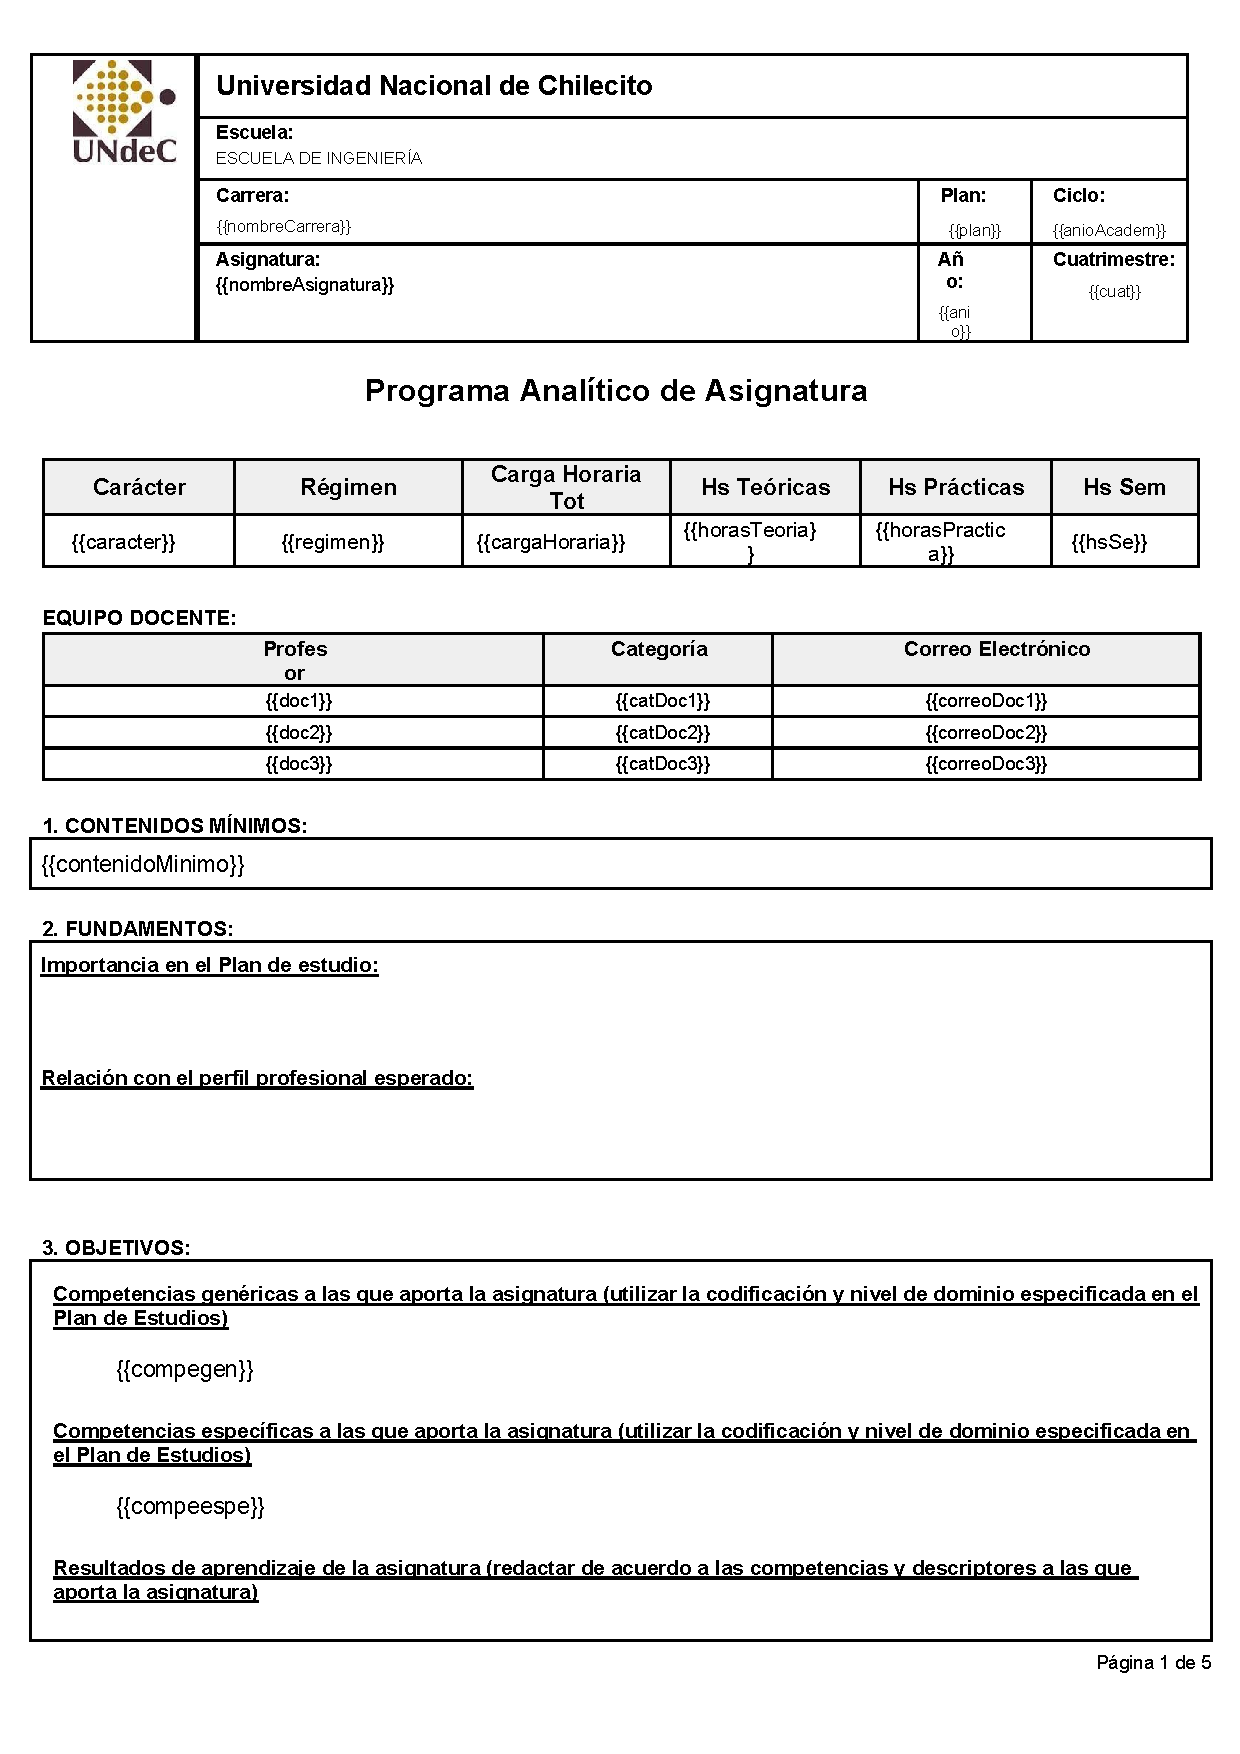
\includepdf[
  pages=-,
  pagecommand={},
  scale=0.82,
  frame=true,
  offset=0 0
]{figures/Template Propuestas.pdf}

%%─────────────────────────────────────────────────────────────────────────────
\chapter{Ejemplos de mensajes MCP (JSON-RPC)}
\label{anexo:mcp_ejemplos}
%%─────────────────────────────────────────────────────────────────────────────

% TODO: Mostrar ejemplos reales o representativos de mensajes MCP:
%
%   Ejemplo 1: Solicitud de tool
%     { "jsonrpc": "2.0", "method": "tools/call", "params": {...}, "id": 1 }
%
%   Ejemplo 2: Respuesta exitosa de tool
%     { "jsonrpc": "2.0", "result": {...}, "id": 1 }
%
%   Ejemplo 3: Invocación de resource
%     { "jsonrpc": "2.0", "method": "resources/read", "params": {...}, "id": 2 }
%
%   Ejemplo 4: Error en mensaje RPC
%     { "jsonrpc": "2.0", "error": {"code": -32601, "message": "Method not found"}, "id": 3 }

\section*{Mensaje de invocación de tool}

Este es un ejemplo de cómo el \textit{Host} invoca un tool a través del MCP Client:

\begin{lstlisting}
{
  "jsonrpc": "2.0",
  "method": "tools/call",
  "params": {
    "name": "extract_proposal",
    "arguments": {"docx_path": "/uploads/proposal.docx"}
  },
  "id": 1
}
\end{lstlisting}

% SECTION: Respuesta de tool
% TODO: Completar con ejemplos reales de respuestas

% SECTION: Manejo de errores
% TODO: Mostrar códigos de error JSON-RPC -32600 a -32603

%%─────────────────────────────────────────────
\chapter{Corpus de evaluación}
\label{anexo:corpus}
%%─────────────────────────────────────────────

% TODO: Describir el corpus en detalle (sin incluir los documentos completos
%   por razones de privacidad institucional):
%   - Tabla con características de las N propuestas evaluadas:
%     Propuesta | Año lectivo | Nº páginas | Nº campos presentes |
%     Formato (DOCX v1/v2/v3) | Observaciones
%   - Distribución de campos presentes/ausentes en el corpus
%   - Ejemplos ANONIMIZADOS de secciones problemáticas para el extractor
%   - Criterios de anotación del ground truth
\ldots

%%─────────────────────────────────────────────
\chapter{Instrucciones de instalación y puesta en marcha}
\label{anexo:instalacion}
%%─────────────────────────────────────────────

% TODO: Guía técnica de instalación para un nuevo entorno:
%   REQUISITOS:
%   - Python 3.11+, Node.js 20+, Git
%   - Clave de API de OpenAI
%
%   BACKEND:
%   cd backend
%   python -m venv .venv
%   .venv\Scripts\activate
%   pip install -r requirements.txt
%   cp .env.example .env   # completar OPENAI_API_KEY
%   python init_db.py
%   uvicorn app.main:app --reload --host 127.0.0.1 --port 8011
%
%   FRONTEND:
%   cd frontend
%   npm install
%   npm run dev -- --host 127.0.0.1 --port 5173
%
%   VERIFICACIÓN:
%   - Backend: http://127.0.0.1:8011/docs (Swagger UI)
%   - Frontend: http://127.0.0.1:5173
%
%   Usar \begin{lstlisting}[language=bash] para los bloques de comando
\ldots


\end{document}
